%-----------------------------------------------------------------------
%
% filename = nube.tex
%
% First version: February 2012
% Last revision: April 2012
%
%-----------------------------------------------------------------------

\documentclass[twocolumn,aps,showpacs,showkeys,prd,superscriptaddress,byrevtex, amsmath]{revtex4-1}


%%%%%%%%%%%%%%%%%%%%%%%%%
%%%   LOAD PACKAGES   %%%
%%%%%%%%%%%%%%%%%%%%%%%%%
 
\usepackage{amssymb}
\usepackage{amsmath}
\usepackage{verbatim}
\usepackage{mathrsfs}
\usepackage{amsfonts}
\usepackage{latexsym}
\usepackage{epsfig}
\usepackage{color}
\usepackage{graphicx,subfigure}
\usepackage{units}
\usepackage{slashbox}
\usepackage{aas_macros}



%%%%%%%%%%%%%%%%%%%%%%%%%
%%%   BEGIN DOCUMENT  %%%
%%%%%%%%%%%%%%%%%%%%%%%%%

\begin{document}


%%%%%%%%%%%%%%%%%%
%%%   MACROS   %%%
%%%%%%%%%%%%%%%%%%

\renewcommand{\t}{\times}
\newcommand{\sg}[1]{\textcolor{blue}{SG: #1}}
\newcommand{\tf}[1]{\textcolor{red}{TF: #1}}

\long\def\symbolfootnote[#1]#2{\begingroup%
\def\thefootnote{\fnsymbol{footnote}}\footnote[#1]{#2}\endgroup}


%%%%%%%%%%%%%%%%%
%%%   TITLE   %%%
%%%%%%%%%%%%%%%%%

\title{Magnetized accretion disks around Kerr black holes with scalar hair - I. Constant angular momentum} 

\author{Sergio Gimeno-Soler}
\affiliation{Departamento de
  Astronom\'{\i}a y Astrof\'{\i}sica, Universitat de Val\`encia,
  C/ Dr. Moliner 50, 46100, Burjassot (Val\`encia), Spain}

\author{Jos\'e A. Font}
\affiliation{Departamento de
  Astronom\'{\i}a y Astrof\'{\i}sica, Universitat de Val\`encia,
  C/ Dr. Moliner 50, 46100, Burjassot (Val\`encia), Spain}
\affiliation{Observatori Astron\`omic, Universitat de Val\`encia, C/ Catedr\'atico 
  Jos\'e Beltr\'an 2, 46980, Paterna (Val\`encia), Spain}

\author{Carlos Herdeiro}
\affiliation{Departamento de F\'{\i}sica da Universidade de Aveiro and CIDMA, Campus de Santiago, 
3810-183 Aveiro, Portugal}

\author{Eugen Radu}
\affiliation{Departamento de F\'{\i}sica da Universidade de Aveiro and CIDMA, Campus de Santiago, 
3810-183 Aveiro, Portugal}


%%%%%%%%%%%%%%%%
%%%   DATE   %%%
%%%%%%%%%%%%%%%%

\date{\today}


%%%%%%%%%%%%%%%%%%%%
%%%   ABSTRACT   %%%
%%%%%%%%%%%%%%%%%%%%

\begin{abstract} 
We present a method to build magnetized constant angular momentum disks around Kerr black holes with scalar hair (KBHsSH).
\end{abstract}


%%%%%%%%%%%%%%%%
%%%   PACS   %%%
%%%%%%%%%%%%%%%%

\pacs{
95.30.Sf, % relativity and gravitation
04.70.Bw, 
04.40.Nr, 
04.25.dg
}


%%%%%%%%%%%%%%%%%%%%%%
%%%   MAKE TITLE   %%%
%%%%%%%%%%%%%%%%%%%%%%

\maketitle


%%%%%%%%%%%%%%%%%%%%%%%%
%%%   INTRODUCTION   %%%
%%%%%%%%%%%%%%%%%%%%%%%%

%%%%%%%%%%%
\section{Introduction}
%%%%%%%%%%%

In recent years, new families of stationary, asymptotically flat black holes (BHs) in general relativity, avoiding the so-called ``no hair" theorems, have been obtained. In particular, Kerr BHs with synchronised hair~\cite{Herdeiro:2014a,Herdeiro:2016} are a counter example to the no hair conjecture, in general relativity minimally coupled to simple (bosonic) matter fields obeying all energy conditions. The physical conditions and stability properties of these {\it hairy} BHs  (HBHs) have been investigated to assess their potential viability as valid alternatives to astrophysical Kerr BHs.  On the one hand, HBHs have been shown to form dynamically as the end-product of the superradiant instability~\cite{East:2017,Herdeiro:2017}. Moreover, the stability of these solutions, questioned by~\cite{Ganchev:2018} in the scalar case, has been recently revisited by~\cite{Degollado:2018} who have shown that the domain of HBH solutions for which the superradiant instability might affect their actual existence has no significance for astrophysical BHs, for the largest timescale possible (the age of the Universe), rendering hairy BHs as {\it effectively} stable.

In addition, the detection of gravitational waves from binary BHs~\cite{Abbott2016, Abbott:2016nmj, Abbott:2017vtc, Abbott:2017oio, Abbott:2017gyy} and the prospect of observing the first image - the black hole {\it shadow} - of a BH by the Event Horizon Telescope~\cite{Fish:2016} opens the opportunity to test the true nature of BHs and the astrophysical relevance of HBHs. 
Regarding the latter, the source of light in a realistic situation is provided by material from an accretion disk crossing the event horizon of the BH, producing the shadow. Thick accretion disks (or tori) are common in astrophysics, either surrounding the central BHs of quasars and active galactic nuclei or, at a stellar scale, surrounding the compact objects in X-ray binaries, microquasars, and gamma-ray bursts. Motivated by this observational possibility, in this work we build equilibrium solutions of HBHs surrounded by magnetized accretion disks. Our procedure, which combines earlier approaches  
by~\cite{Komissarov:2006,Qian:2009} was presented in~\cite{Gimeno-Soler:2017} for the Kerr BH case. In~\cite{Gimeno-Soler:2017} we built equilibrium sequences of accretion disks  endowed with a purely toroidal magnetic field, assuming a form of the angular momentum distribution that departs from the constant case considered by~\cite{Komissarov:2006} and from which the location and morphology of the equipotential surfaces can be numerically computed. Our immediate goal in the present work is to assess if and how the accretion disk morphology depends on the type of BH considered, either Kerr BHs of varying spins or Kerr BHs with scalar hair (KBHsSH). Moreover, we focus on disks with a constant distribution of specific angular momentum, presenting in a companion paper the non-constant (power-law) case. In subsequent investigations, we will analyze the shadows of the equilibrium models of KBHsSH presented in this work as well as in {\it dynamical} situations.

The organization of this paper is as follows: Section~\ref{framework} presents  the  analytic  mathematical framework to build non-self-gravitating magnetized discs in the spacetime of KBHsSH. Section~\ref{procedure} discusses the corresponding numerical methodology. The sequences of equilibrium models are presented and  discussed in Section~\ref{results}. Finally, our conclusions  are  summarized  in  Section~\ref{conclusions}.  
 

%HERE

%%%%%%%%%%%
\section{Framework}
\label{framework}
%%%%%%%%%%%

%%%%%%%%%%%%%%%%%%%%%%%%%%%
\subsection{Spacetime metric and KBHsSH models}
%%%%%%%%%%%%%%%%%%%%%%%%%%%


%%%%%%%%%%%%%%%%%%%
\begin{table*}
\caption{List of models of KBHsSH used in this work. From left to right the columns report the name of the model, the ADM mass, $M_{\mathrm{ADM}}$, the ADM angular momentum, $J_{\mathrm{ADM}}$, the horizon mass, $M_{\mathrm{H}}$, the horizon angular momentum, $J_{\mathrm{H}}$, the mass of the scalar field, $M_{\mathrm{SF}}$, the angular momentum of the scalar field, $J_{\mathrm{SF}}$, the radius of the event horizon, $r_{\mathrm{H}}$, the values of the normalized spin parameter for the ADM quantities, $a_{\mathrm{ADM}}$, and for the BH horizon quantities, $a_{\mathrm{H}}$, the horizon linear velocity, $v_{\mathrm{H}}$, and the spin parameter corresponding to a Kerr BH with a linear velocity equal to $v_{\mathrm{H}}$, $a_{\mathrm{H_{eq}}}$.}        
\label{models_list}      
\centering          
\begin{tabular}{c c c c  c c c c   c c c c}
\hline\hline       
 Model & $M_{\mathrm{ADM}}$ & $J_{\mathrm{ADM}}$ & $M_{\mathrm{H}}$ &  $J_{\mathrm{H}}$ & $M_{\mathrm{SF}}$ & $J_{\mathrm{SF}}$ & $r_{\mathrm{H}}$ & $a_{\mathrm{ADM}}$ & $a_{\mathrm{H}}$ & $v_{\mathrm{H}}$ & $a_{\mathrm{H_{eq}}}$ \\ 
\hline           
I & $0.415$ & $0.172$ & $0.393$ &  $0.15$  & $0.022$ & $0.022$ & $0.200$ & $0.9987$ & $0.971$ & $0.7685$ & $0.9663$\\ 
 \hline 
II & $0.630$ & $0.403$ & $0.340$ &  $0.121$  & $0.063$ & $0.282$ & $0.221$ & $1.0140$ & $0.376$ & $0.6802$ & $0.9301$ \\
 \hline 
III & $0.797$ & $0.573$ & $0.365$ &  $0.172$  & $0.573$ & $0.432$ & $0.111$ & $0.9032$ & $1.295$ & $0.7524$ & $0.9608$ \\ 
 \hline 
IV & $0.933$ & $0.739$ & $0.234$ &  $0.114$  & $0.699$ & $0.625$ & $0.100$ & $0.8489$ & $2.082$ & $0.5635$ & $0.8554$ \\ 
 \hline 
V & $0.940$ & $0.757$ & $0.159$ &  $0.076$  & $0.757$ & $0.781$ & $0.091$ & $0.8560$ & $3.017$ & $0.4438$ & $0.7415$ \\ 
 \hline 
VI & $0.959$ & $0.795$ & $0.087$ &  $0.034$  & $0.872$ & $0.781$ & $0.088$ & $0.9477$ & $3.947$ & $0.2988$ & $0.5487$ \\ 
 \hline 
VII & $0.975$ & $0.850$ & $0.018$ &  $0.002$  & $0.957$ & $0.848$ & $0.040$ & $0.8941$ & $6.173$ & $0.0973$ & $0.1928$ \\ 
\hline      
\end{tabular}
\end{table*}
%%%%%%%%%%%%%%%%%%%


The KBHsSH models we use in this study are built following the procedure described in~\cite{Herdeiro:2015b}. The underlying theoretical framework is the Einstein-Klein-Gordon (EKG) field theory, describing a massive complex scalar field $\Psi$ minimally coupled to Einstein gravity. KBHsSH solutions are obtained by using the following ansatz for the metric and the scalar field~\cite{Herdeiro:2014a}
\begin{eqnarray}
%\begin{split}
\mathrm{d}s^2 &=& e^{2F_1}\left(\frac{\mathrm{d}r^2}{N} + r^2\mathrm{d}\theta^2\right) +  e^{2F_2}r^2\sin^2 \theta(\mathrm{d}\phi-W\mathrm{d}t)^2 
\nonumber \\ 
&-&  e^{2F_0}N\mathrm{d}t^2\,,
\label{metric}
\end{eqnarray}
\begin{eqnarray}
\Psi = \phi(r, \theta) e^{\mathrm{i}(m\varphi - \omega t)} \,,
%\end{split}
\end{eqnarray}
with $N = 1 - r_H/r$, where $r_H$ is the radius of the event horizon of the BH, and $W$, $F_1$, $F_2$, $F_0$ are functions of $r$ and $\theta$. Moreover, $\omega$ is the scalar field frequency and $m$ is the azimuthal harmonic index.

The stationary and axisymmetric metric ansatz is a solution to the EKG field equations $R_{ab} - \frac{1}{2}R g _{ab} = 8 \pi G (T_{\mathrm{SF}})_{ab}$ with 
\begin{eqnarray}\label{eq:e-m_scalaf_field}
(T_{\mathrm{SF}})_{ab} &=& \partial_a \Psi^* \partial_b \Psi + \partial_b \Psi^* \partial_a \Psi 
\nonumber \\ 
&-& g_{ab} \left(\frac{1}{2} g^{cd}(\partial_c \Psi^* \partial_d \Psi + \partial_d \Psi^* \partial_c \Psi) + \mu^2 \Psi^* \Psi \right),
\end{eqnarray}
where $\mu$ is the mass of the scalar field and $^*$ denotes complex conjugation. The interested reader is addressed to~\cite{Herdeiro:2015b} for details on the equations of motion for the scalar field $\Psi$ and the four metric functions ${W, F_i}$, along with their solution.

Table~\ref{models_list} lists the seven KBHsSH models we use in this work. The models have been selected to span all regions of interest in the parameter space. Model I corresponds to a Kerr-like model, with almost all the mass and angular momentum stored in the BH, while model VII corresponds to a KBHSH with almost all the mass and angular momentum stored in the scalar field. It is worth mentioning that some of the models violate the Kerr bound (normalized sìn parameter larger than 1) in terms of both ADM or horizon quantities. This is not a source of concern because, as shown in~\cite{Herdeiro:2015c} the linear velocity of the horizon, $v_{\mathrm{H}}$, never exceeds $1$. For comparison, we also show in the last column of Table~\ref{models_list} the spin parameter $a_{\mathrm{H_{eq}}}$ corresponding to a Kerr BH with a horizon linear velocity $v_{\mathrm{H}}$. \tf{Further description of the table. Something must be said about the coordinates.}. In addition to the information provided in Table~\ref{models_list}, Figure~\ref{existence} plots the location of our models in  the domain of existence of KBHsSH in an ADM mass versus scalar field frequency diagram. 



%\begin{table}
%\caption{Values of the normalized spin parameter for the ADM quantities ($a_{\mathrm{ADM}}$), for the BH horizon quantities ($a_{\mathrm{H}}$), the horizon linear velocity ($v_{\mathrm{H}}$) and the spin parameter corresponding to a KBH with a linear velocity equal to $v_{\mathrm{H}}$, ($a_{\mathrm{H_{eq}}}$).}        
%\label{models_spin_vel}      
%\centering          
%\begin{tabular}{c c c c c}
%\hline\hline       
% Model & $a_{\mathrm{ADM}}$ & $a_{\mathrm{H}}$ & $v_{\mathrm{H}}$ & $a_{\mathrm{H_{eq}}}$ \\ 
%\hline           
%I & $0.9987$ & $0.9712$ & $0.7685$ & $0.9663$ \\ 
% \hline 
%II & $1.014$ & $0.3760$ & $0.6802$ & $0.9301$ \\
% \hline 
%III & $0.9032$ & $1.295$ & $0.7524$ & $0.9608$ \\ 
% \hline 
%IV & $0.8489$ & $2.082$ & $0.5635$ & $0.8554$ \\ 
% \hline 
%V & $0.8560$ & $3.017$ & $0.4438$ & $0.7415$ \\ 
% \hline 
%VI & $0.9477$ & $3.947$ & $0.2988$ & $0.5487$ \\ 
% \hline 
%VII & $0.8941$ & $6.173$ & $0.09732$ & $0.1928$ \\ 
%\hline      
%\end{tabular}
%\end{table}

\begin{figure}
\centering
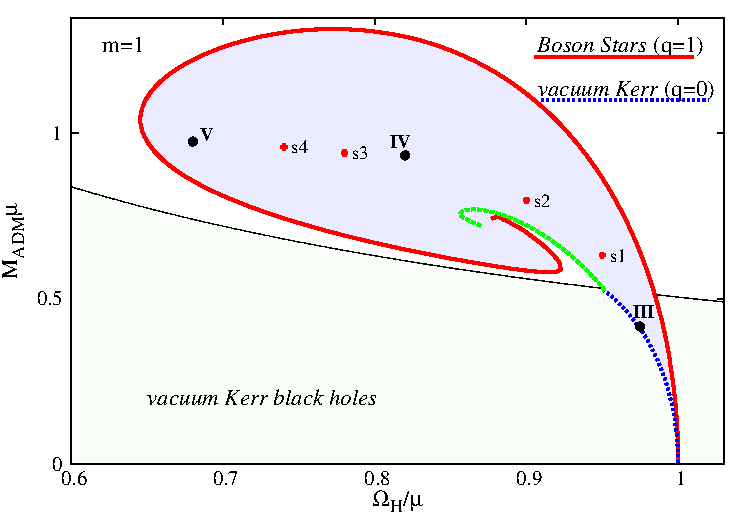
\includegraphics[scale=0.7]{figures/existence-eps-converted-to.pdf}
\caption{Domain of existence for KBHsSH in an ADM mass versus scalar
field frequency diagram. \tf{The figure has to be redone to label the 7 models used in this work.}}
\label{existence}
\end{figure}


\begin{figure*}
\centering
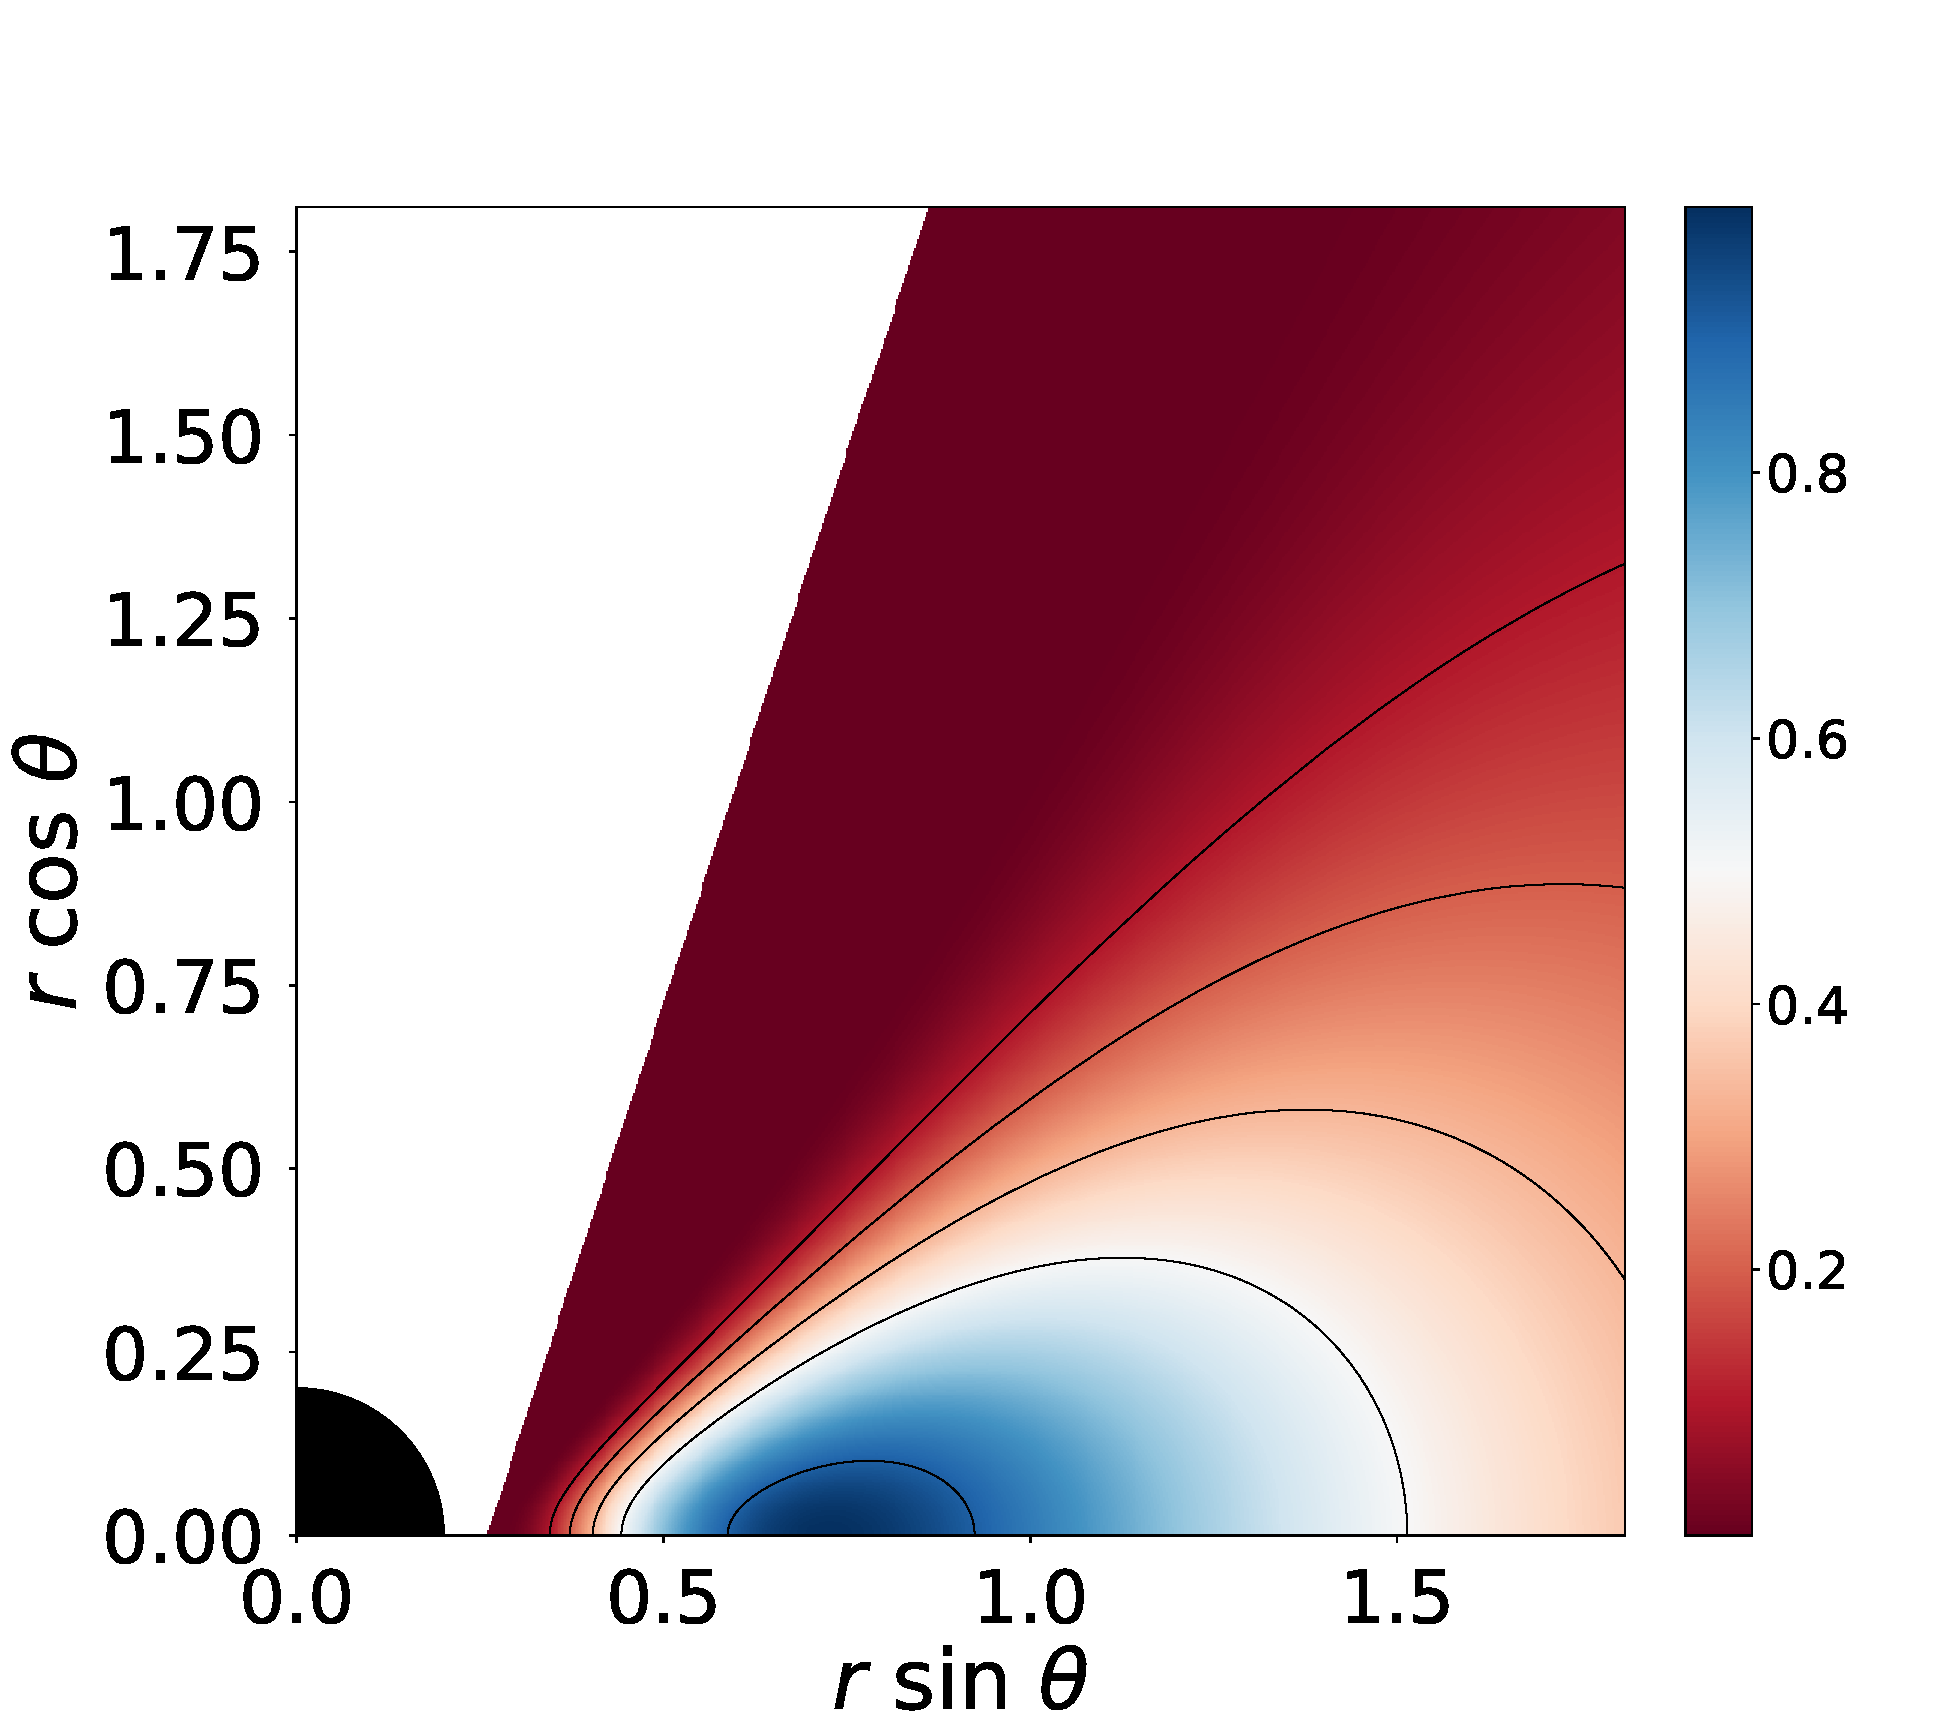
\includegraphics[scale=0.14]{figures/fig1_I_10.pdf}
\hspace{-0.3cm}
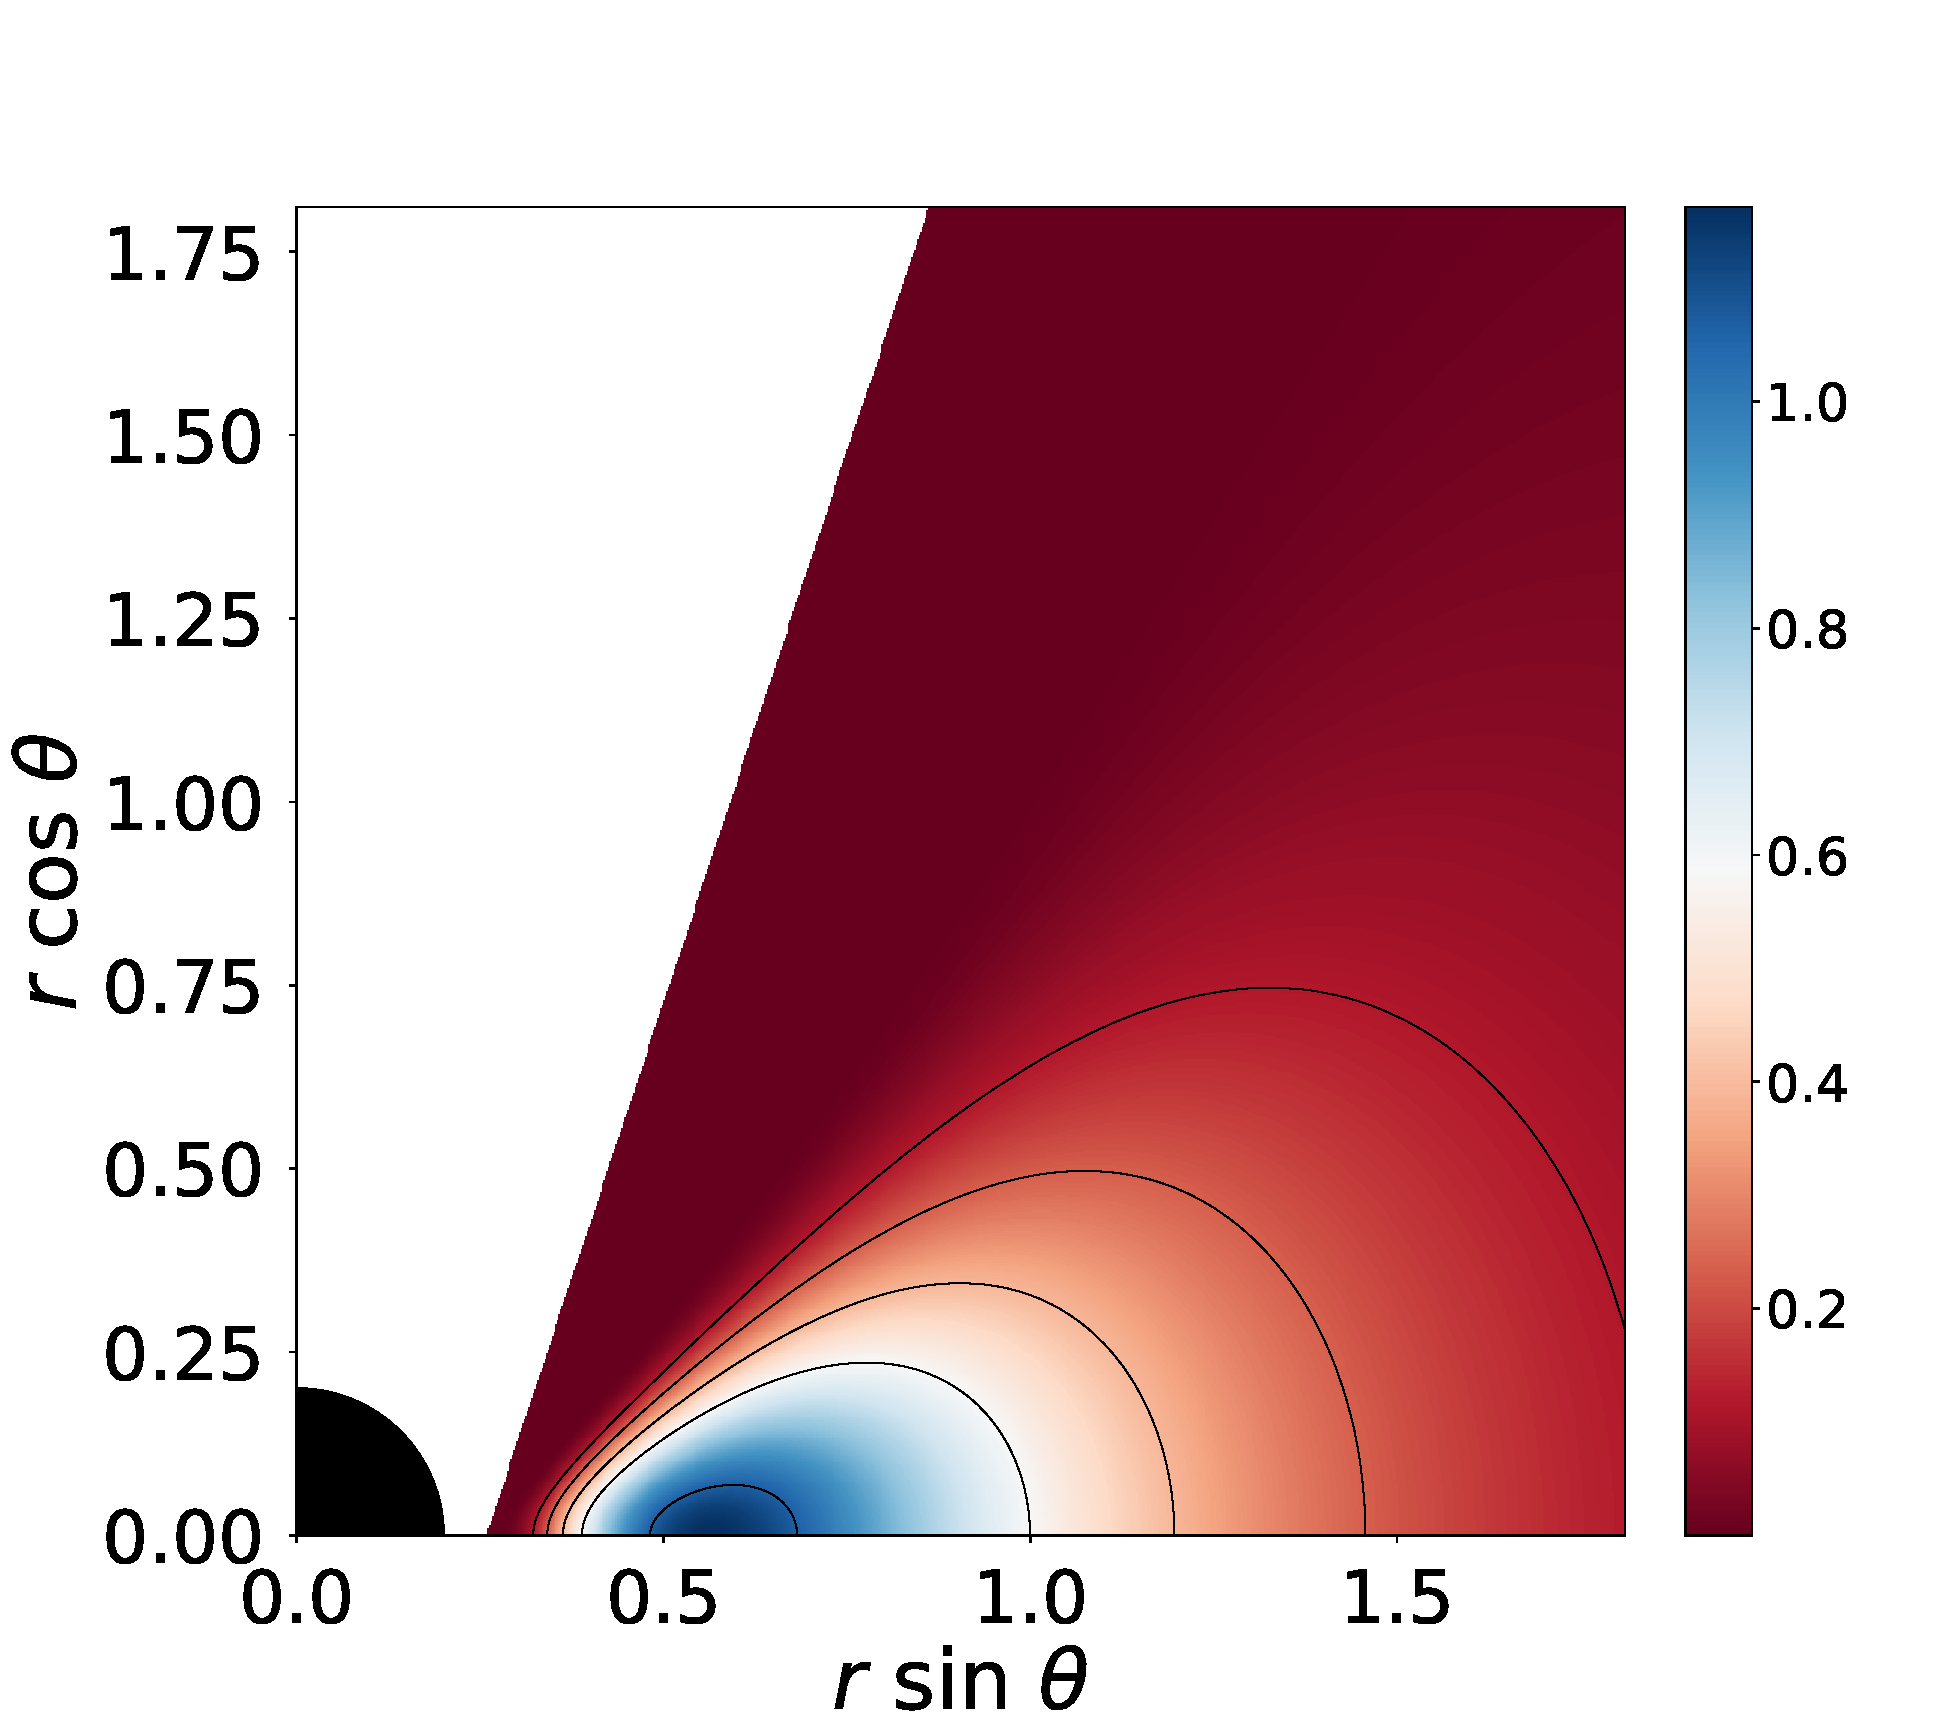
\includegraphics[scale=0.14]{figures/fig1_I_1.pdf}
\hspace{-0.2cm}
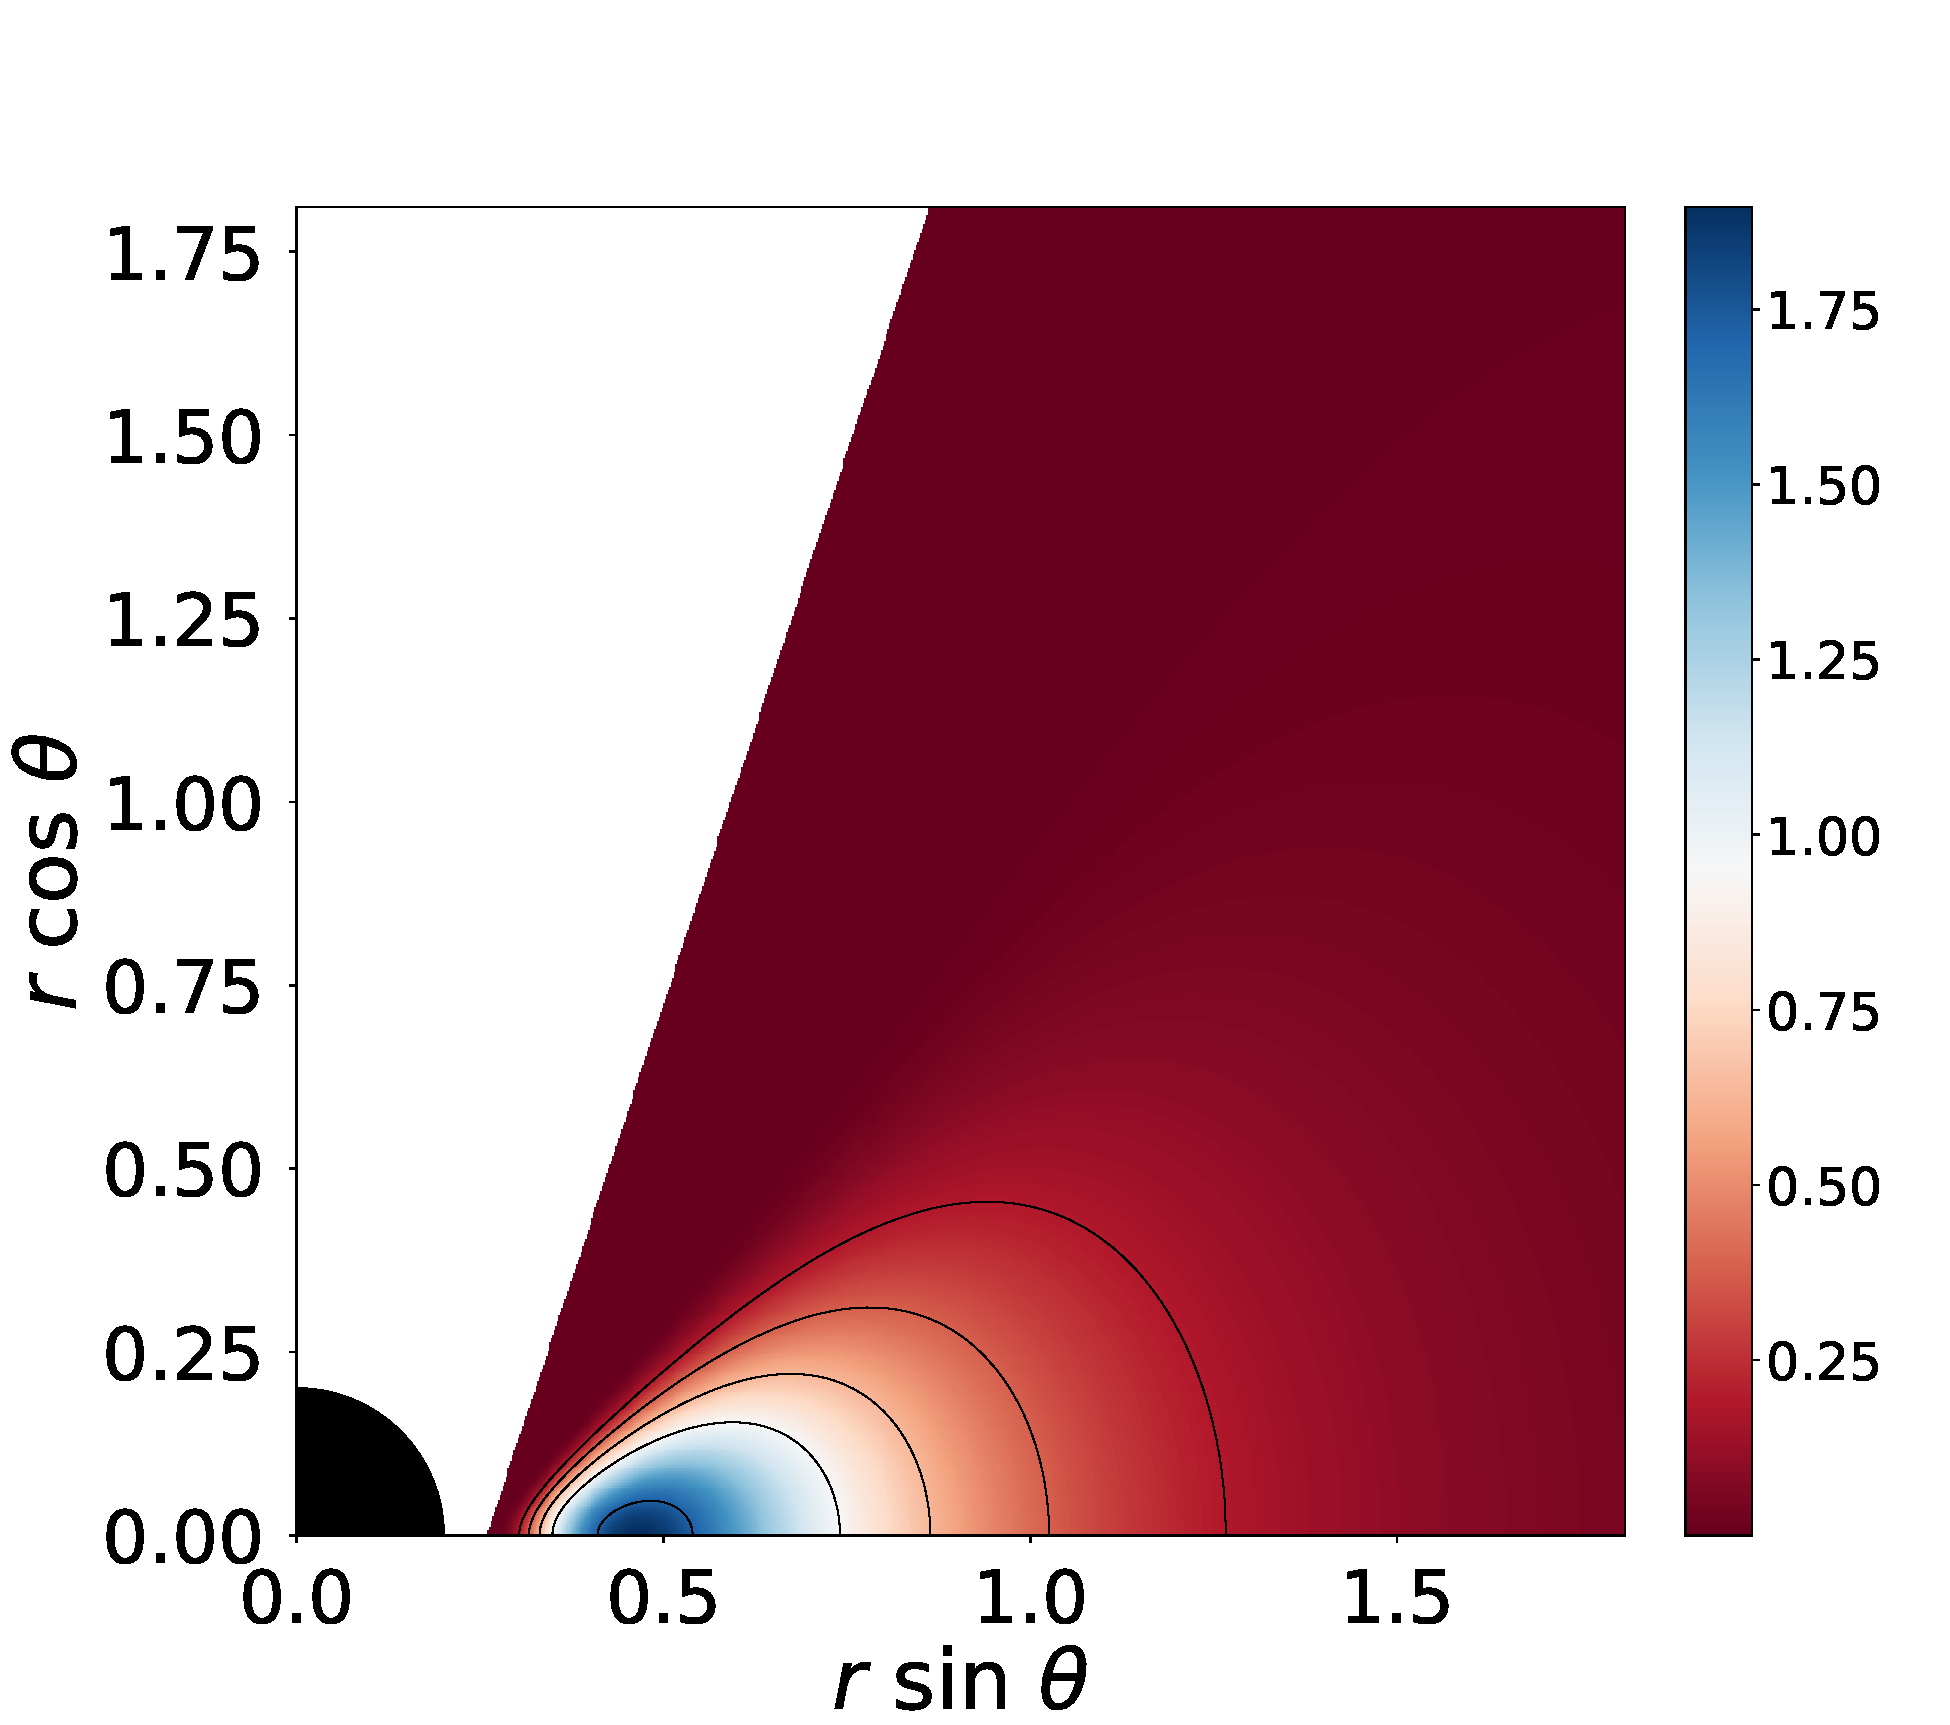
\includegraphics[scale=0.14]{figures/fig1_I__10.pdf}
\\
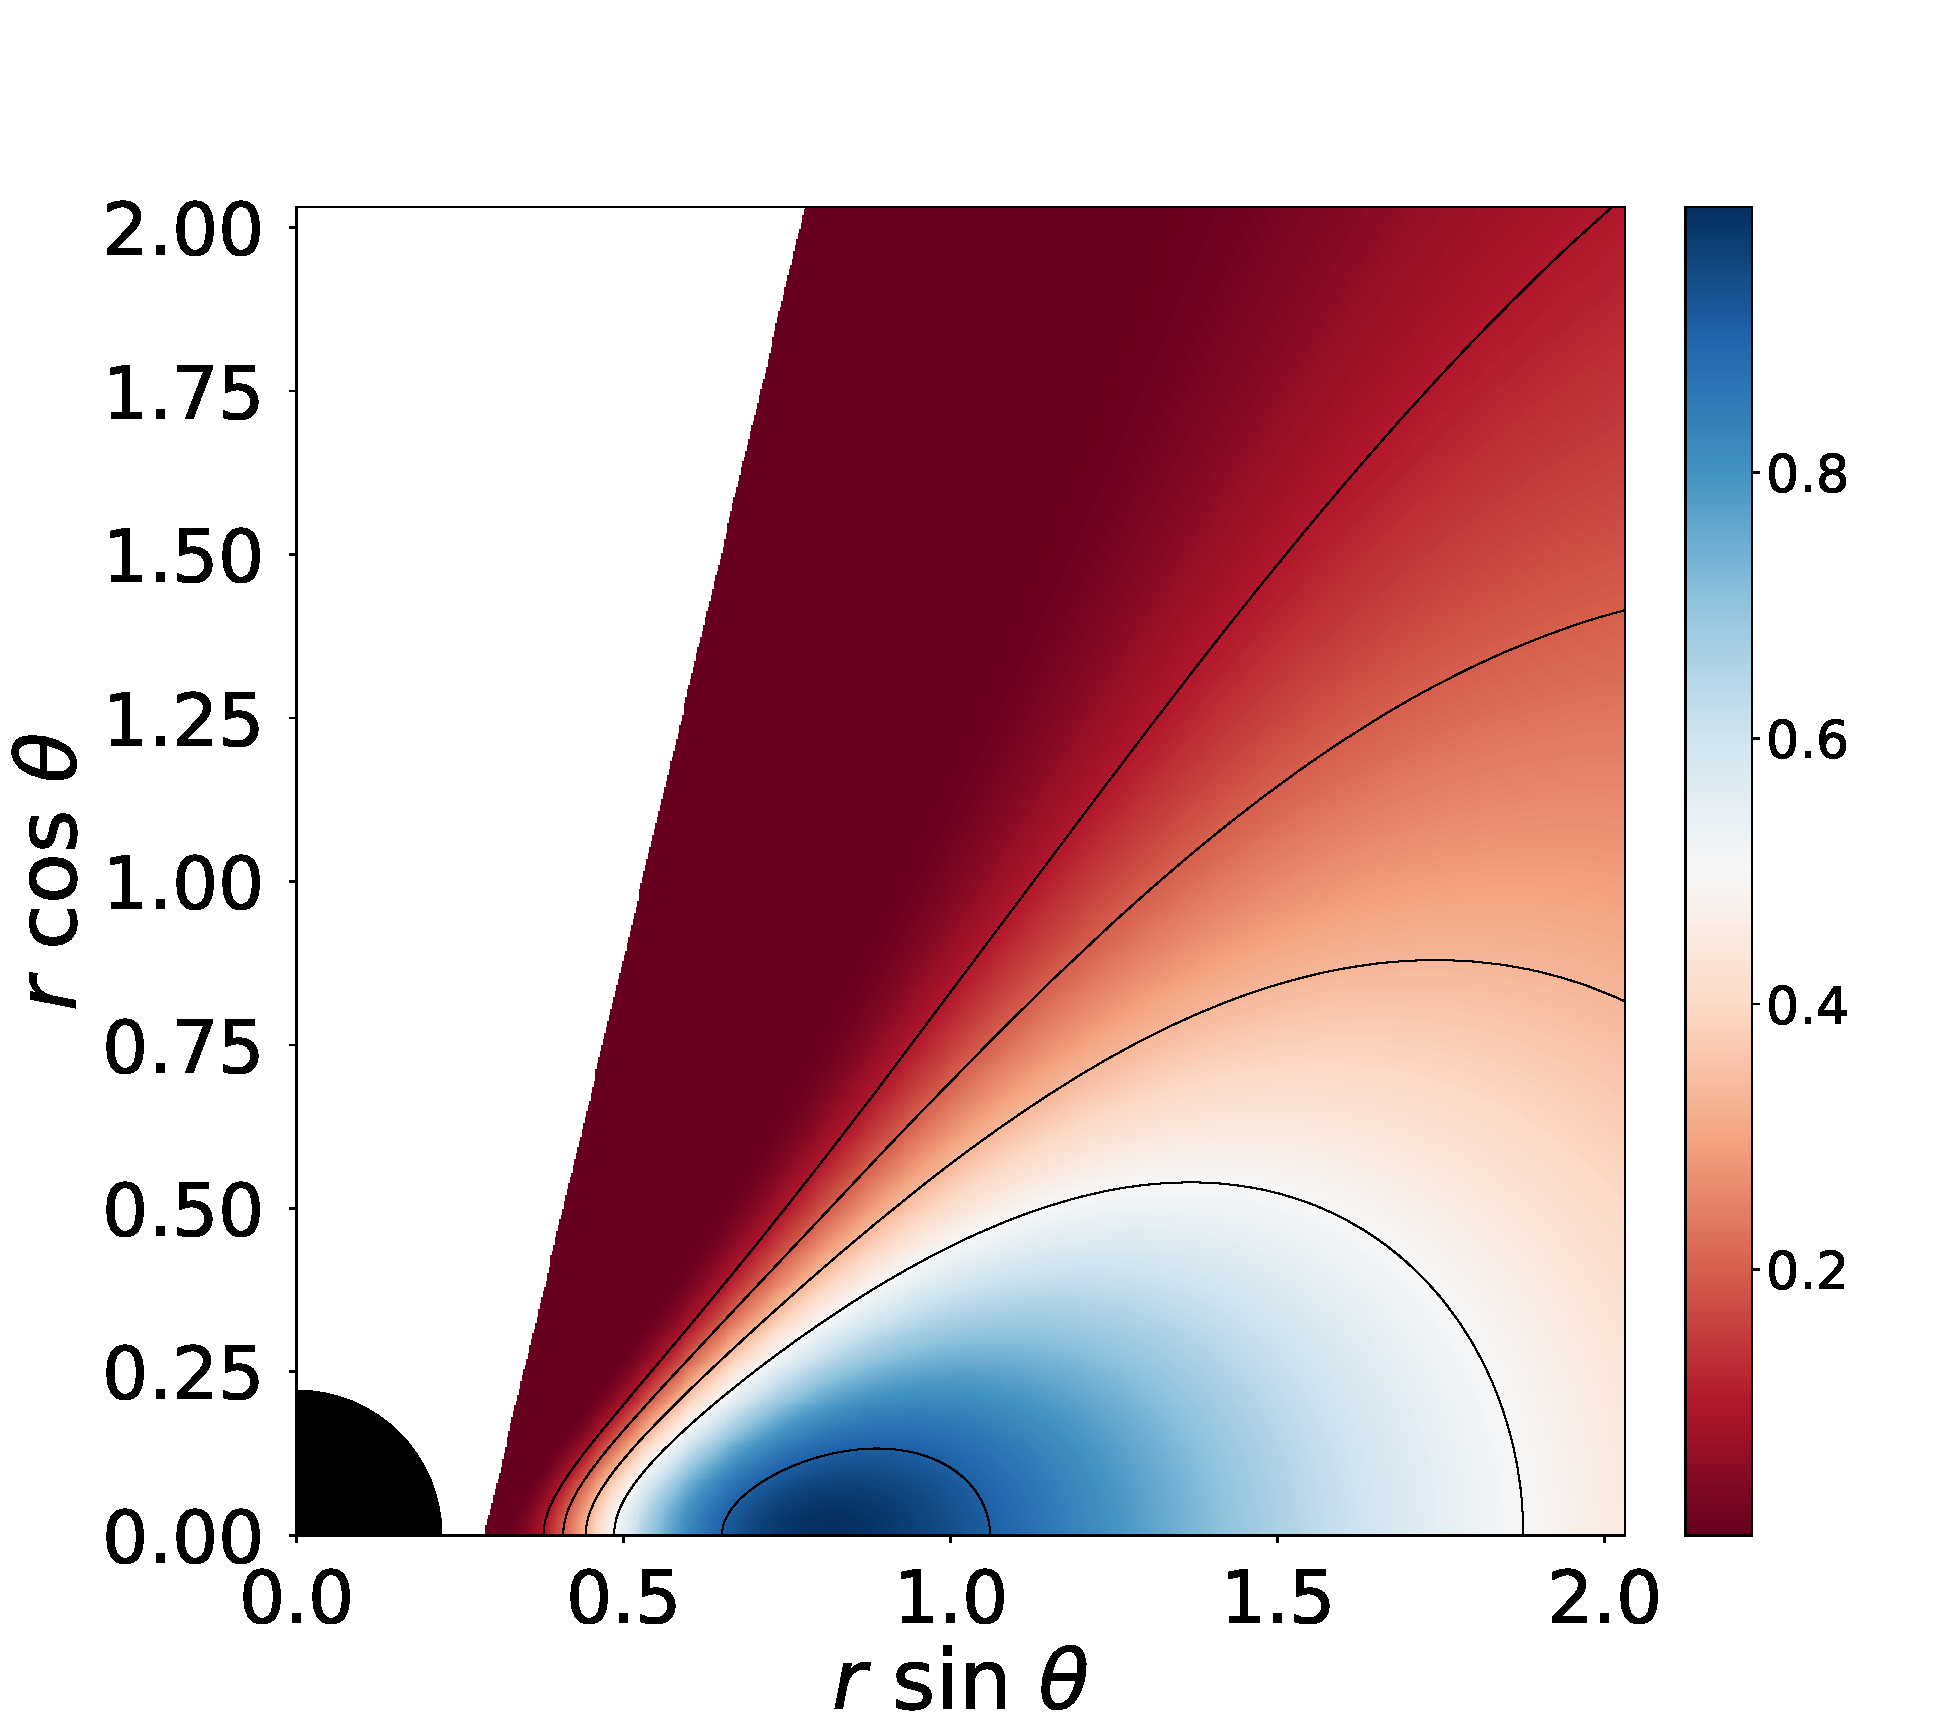
\includegraphics[scale=0.14]{figures/fig1_II_10.pdf}
\hspace{-0.3cm}
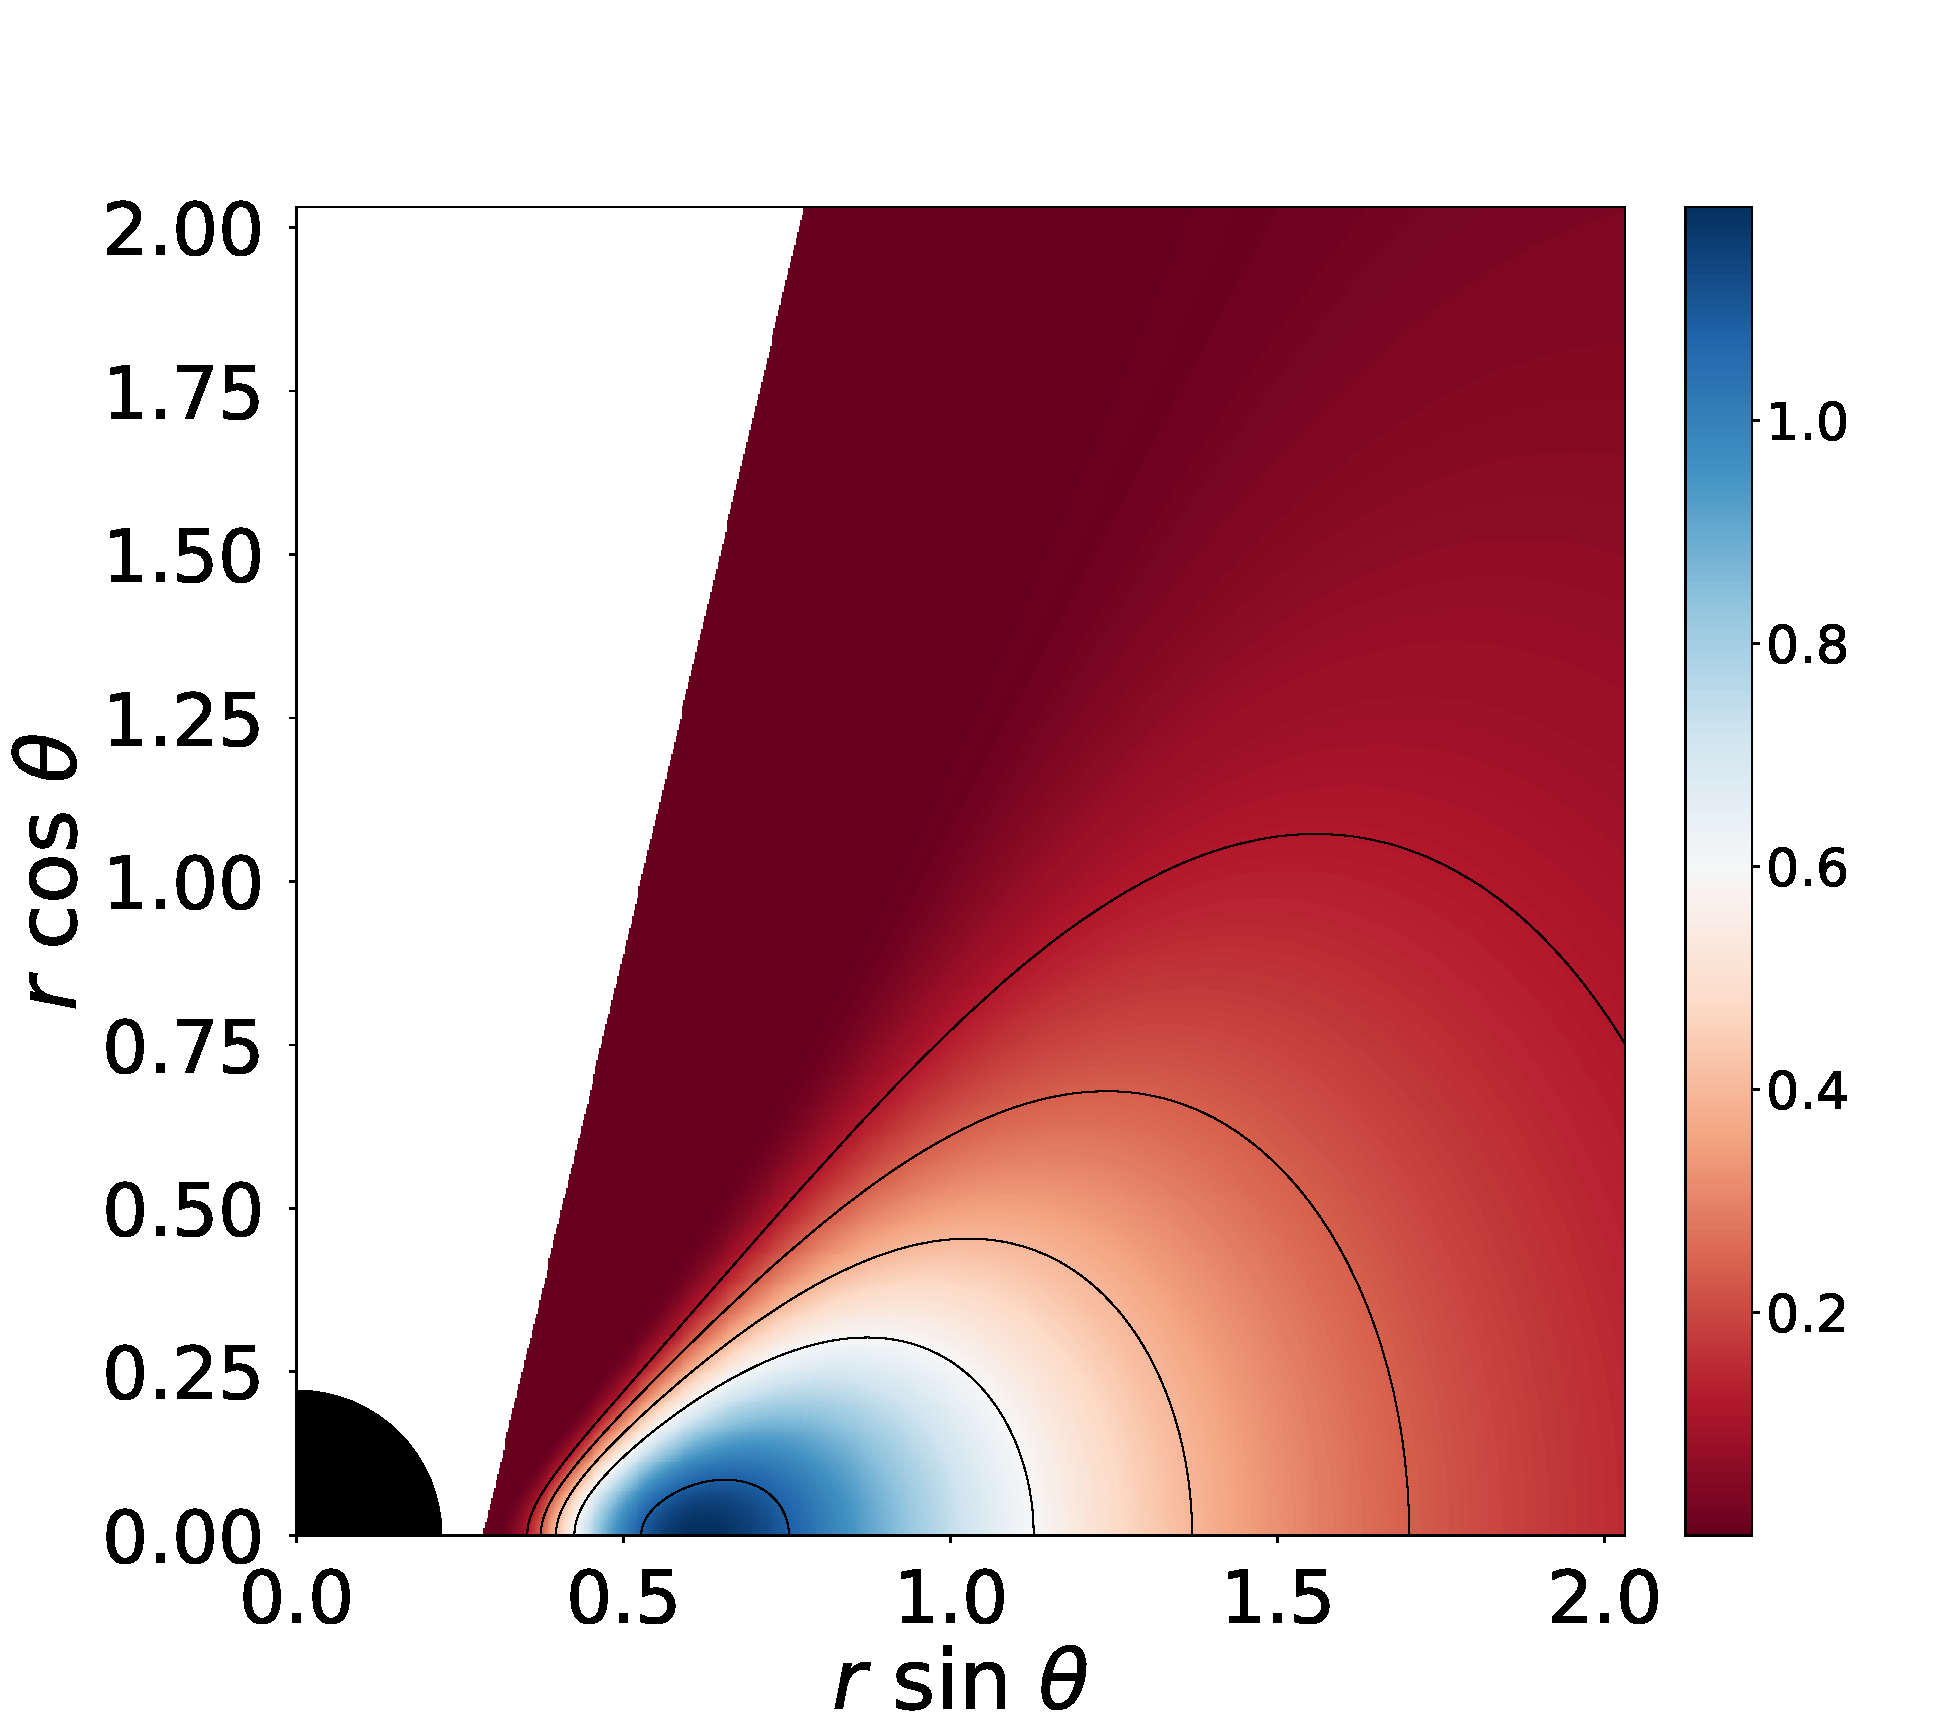
\includegraphics[scale=0.14]{figures/fig1_II_1.pdf}
\hspace{-0.2cm}
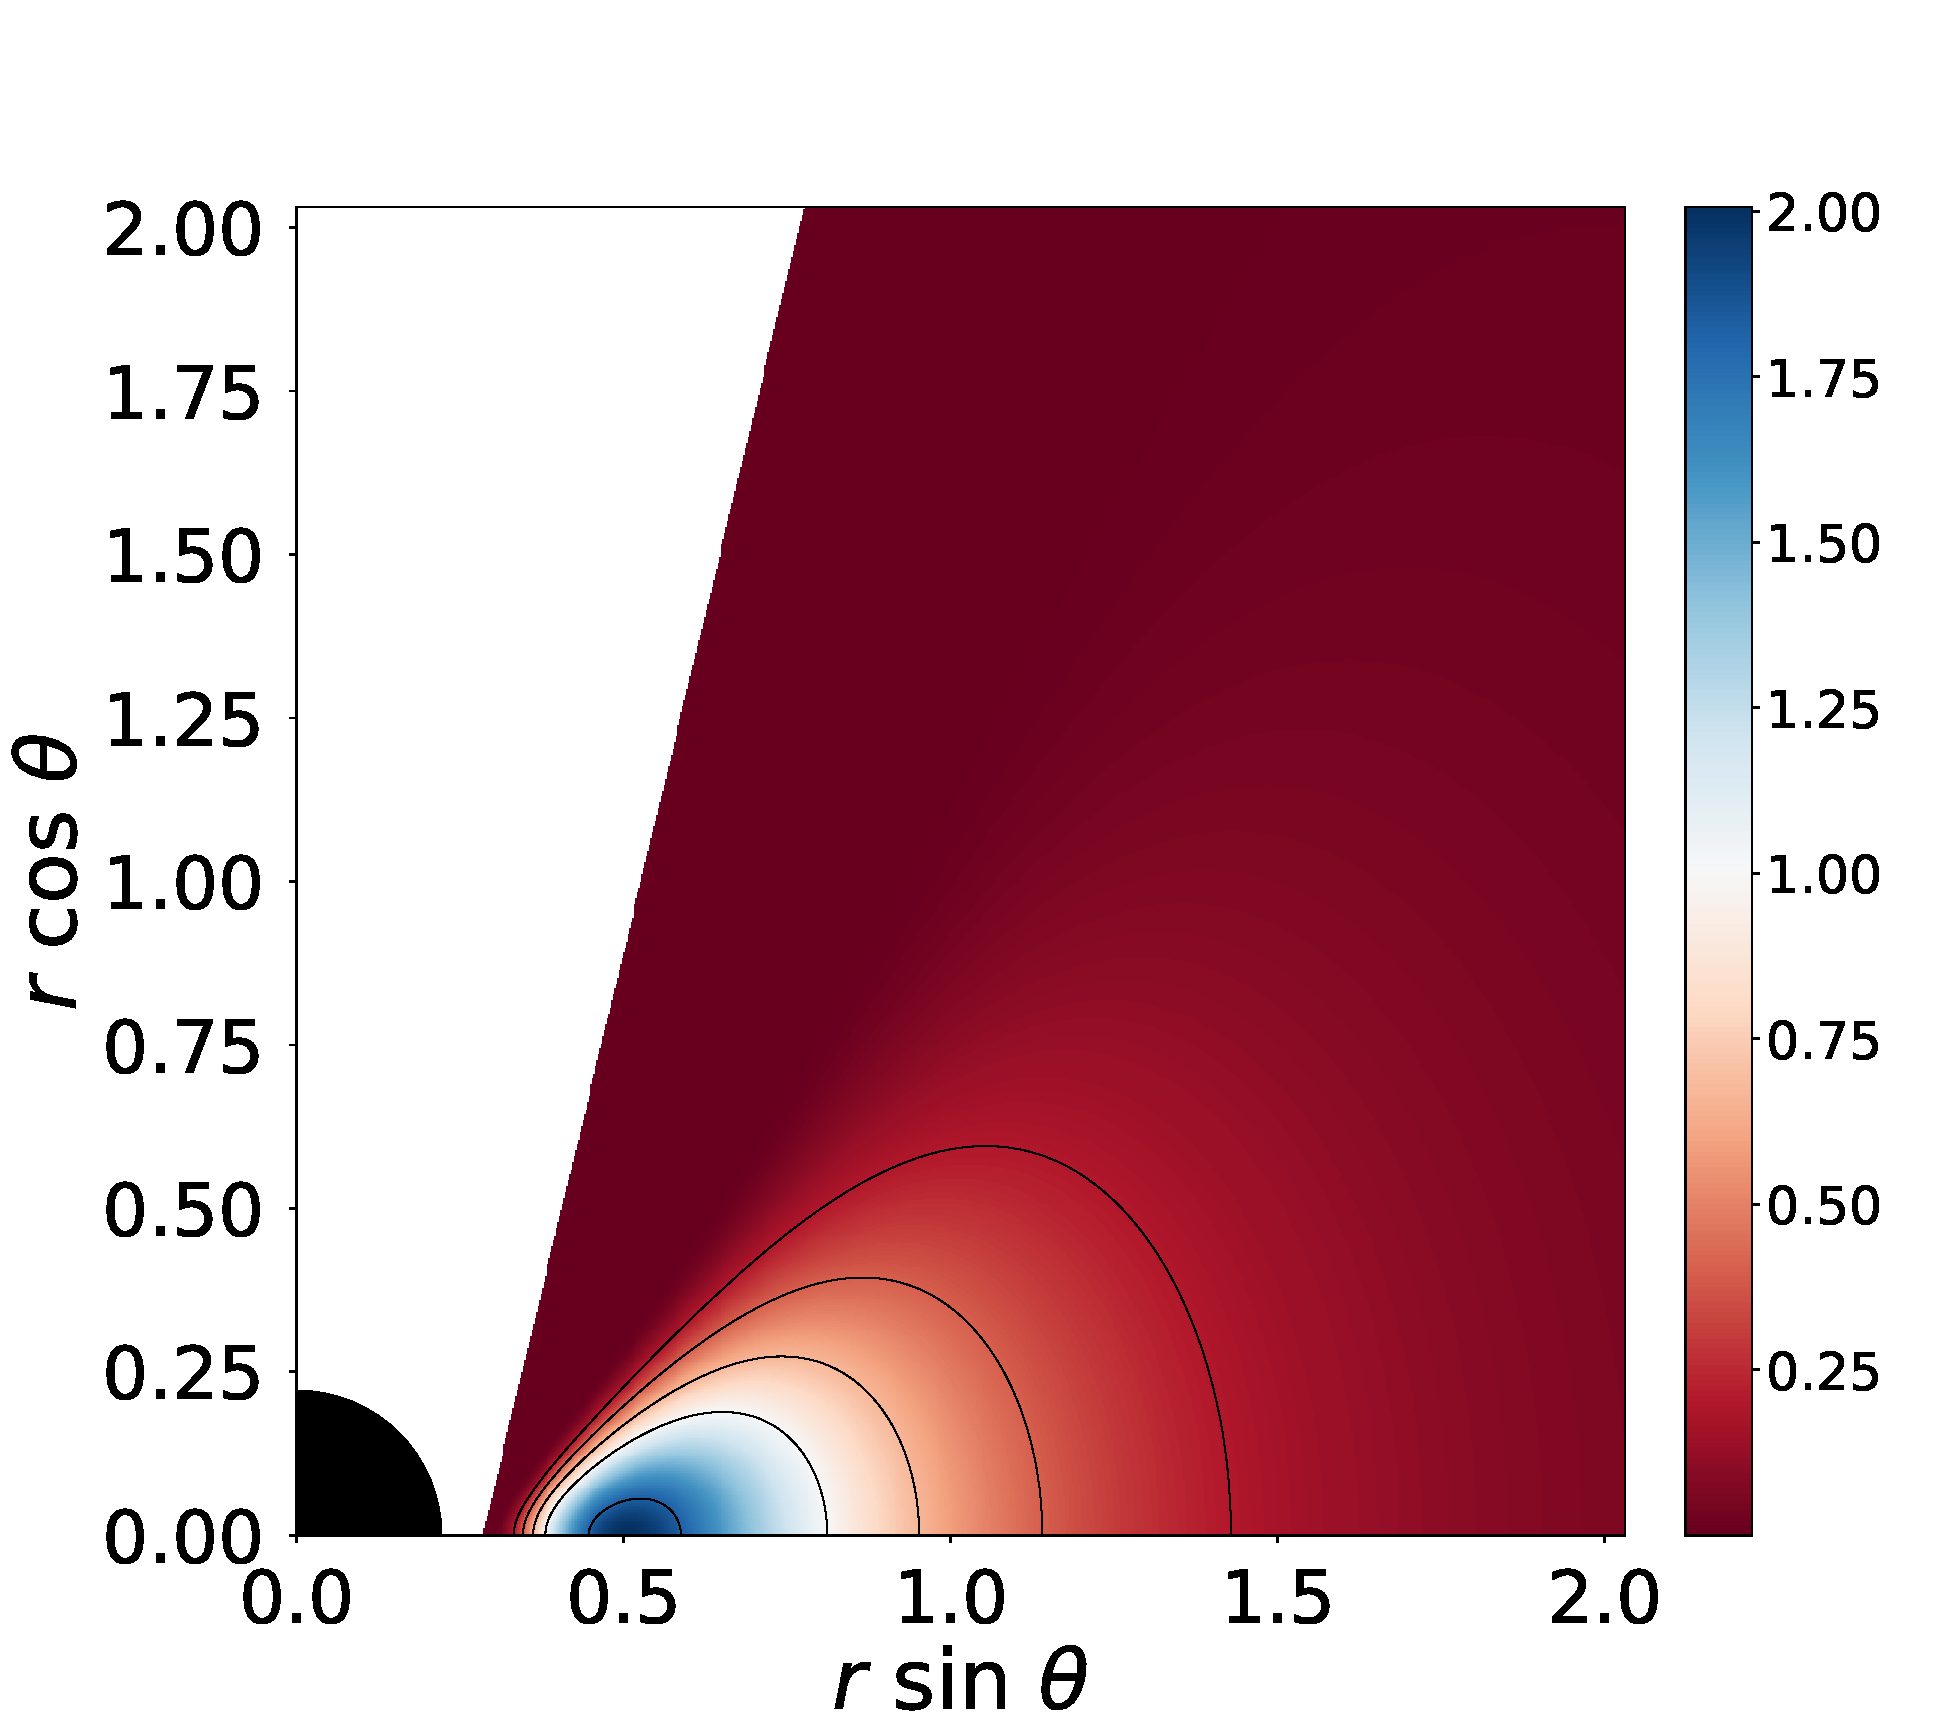
\includegraphics[scale=0.14]{figures/fig1_II__10.pdf}
\\
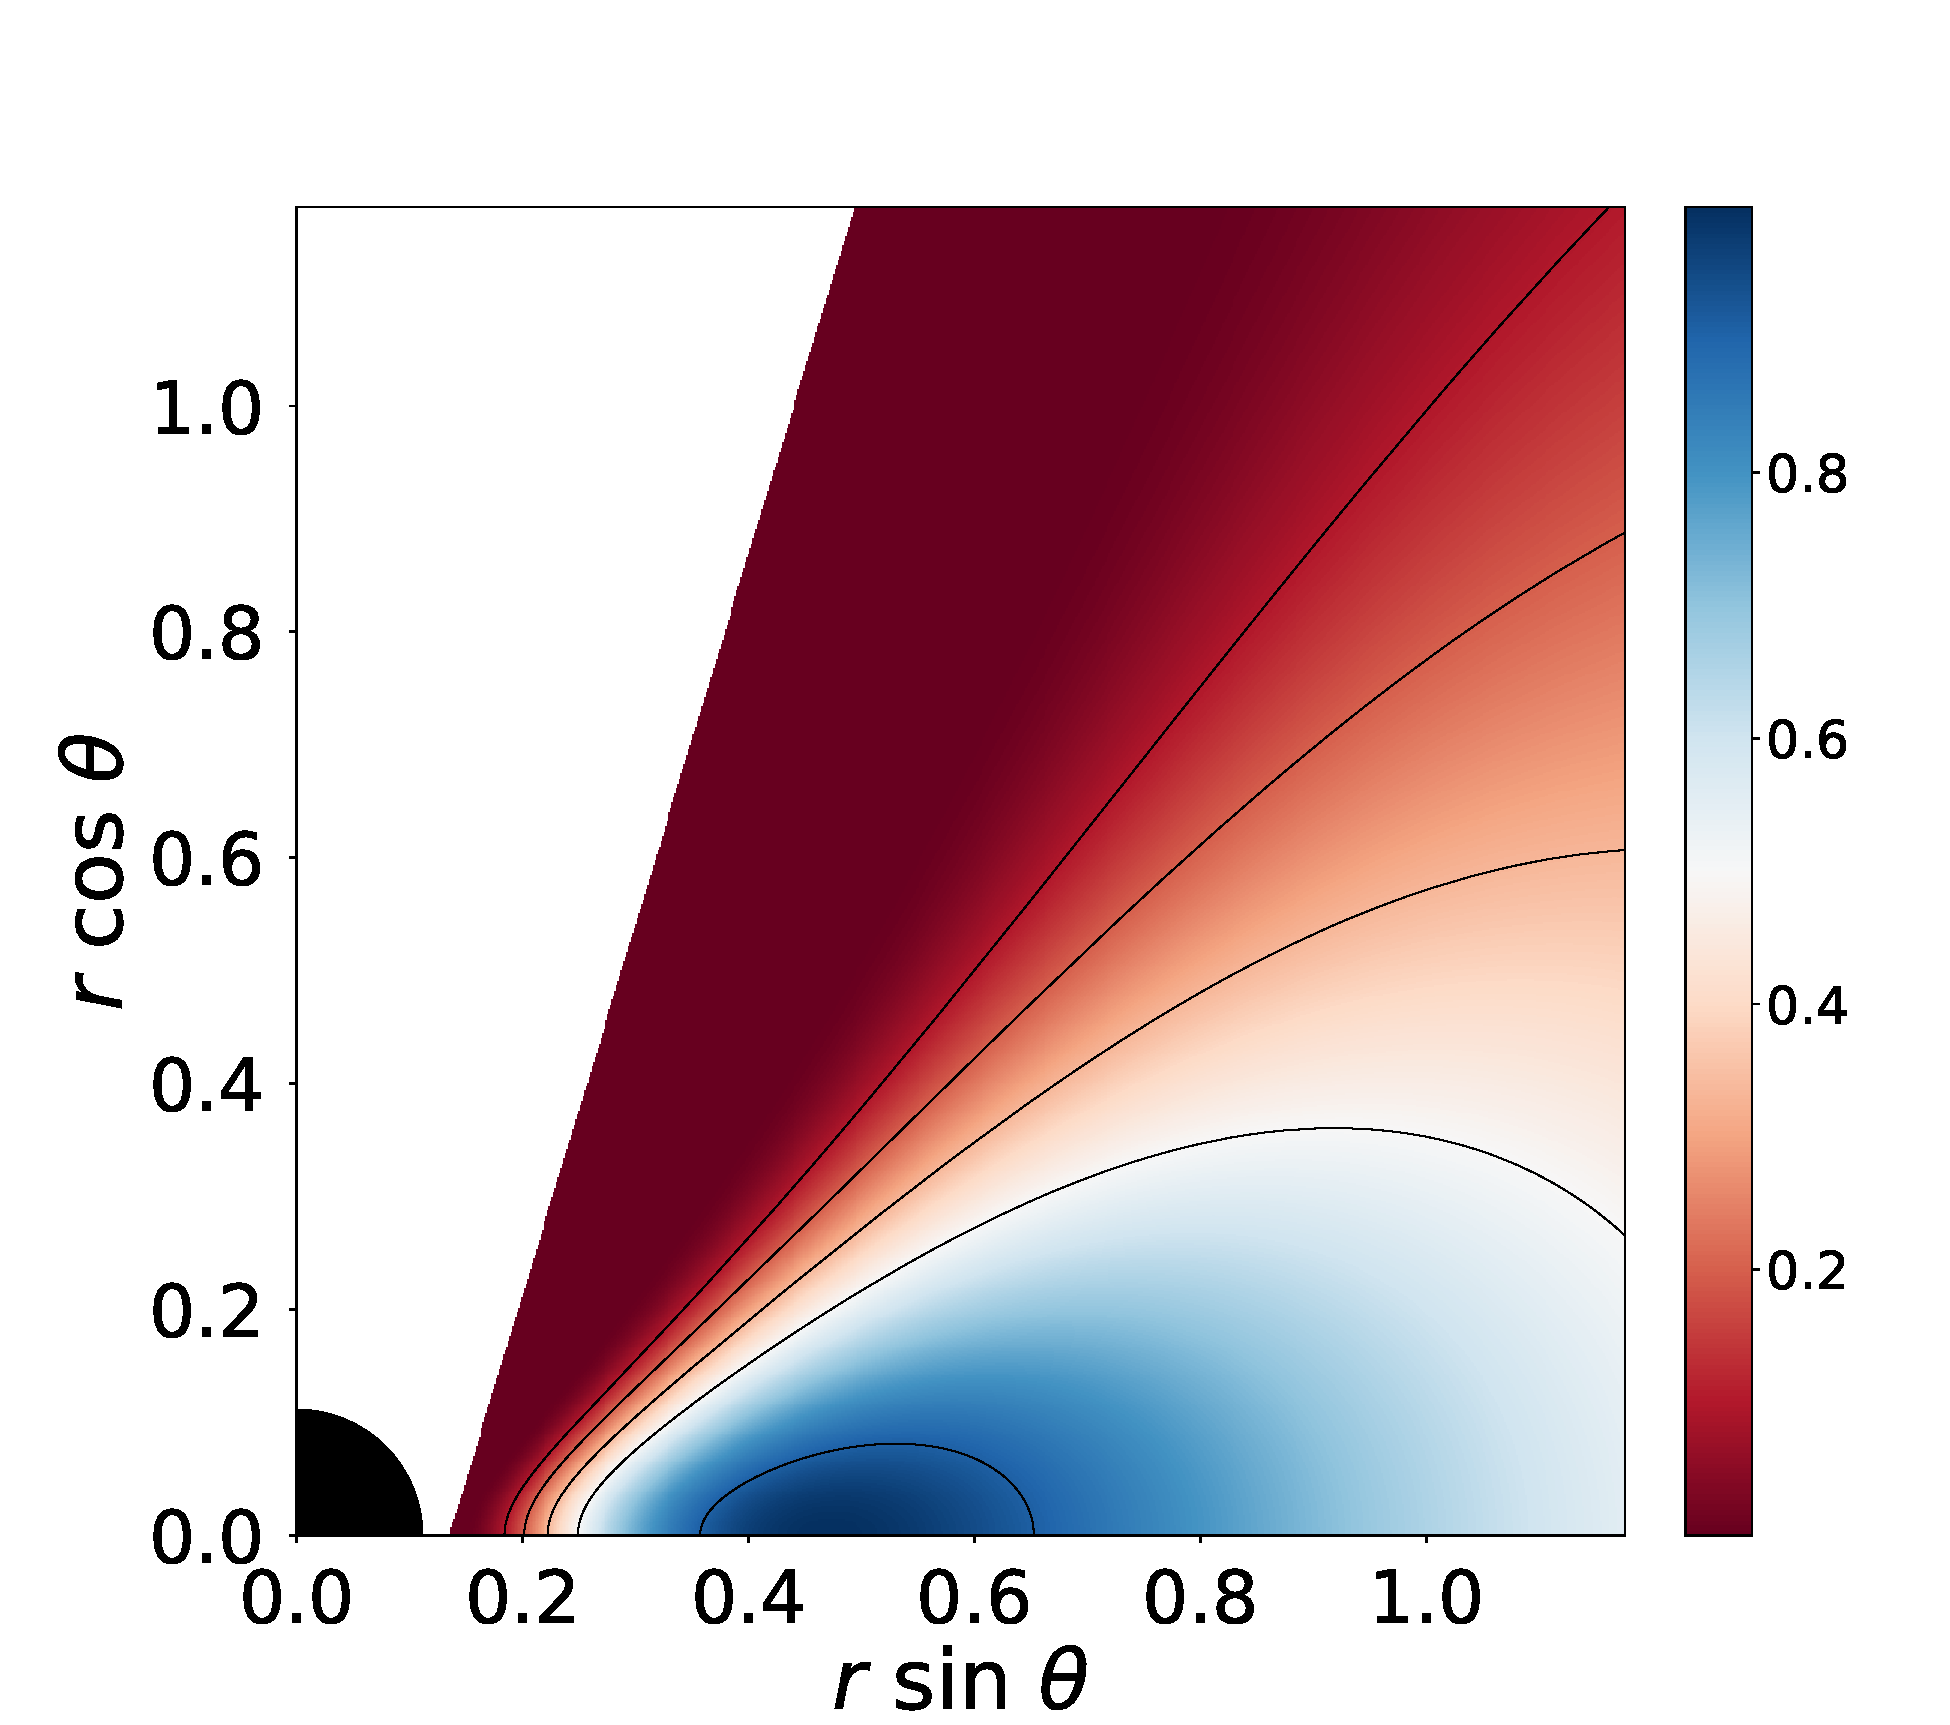
\includegraphics[scale=0.14]{figures/fig1_III_10.pdf}
\hspace{-0.3cm}
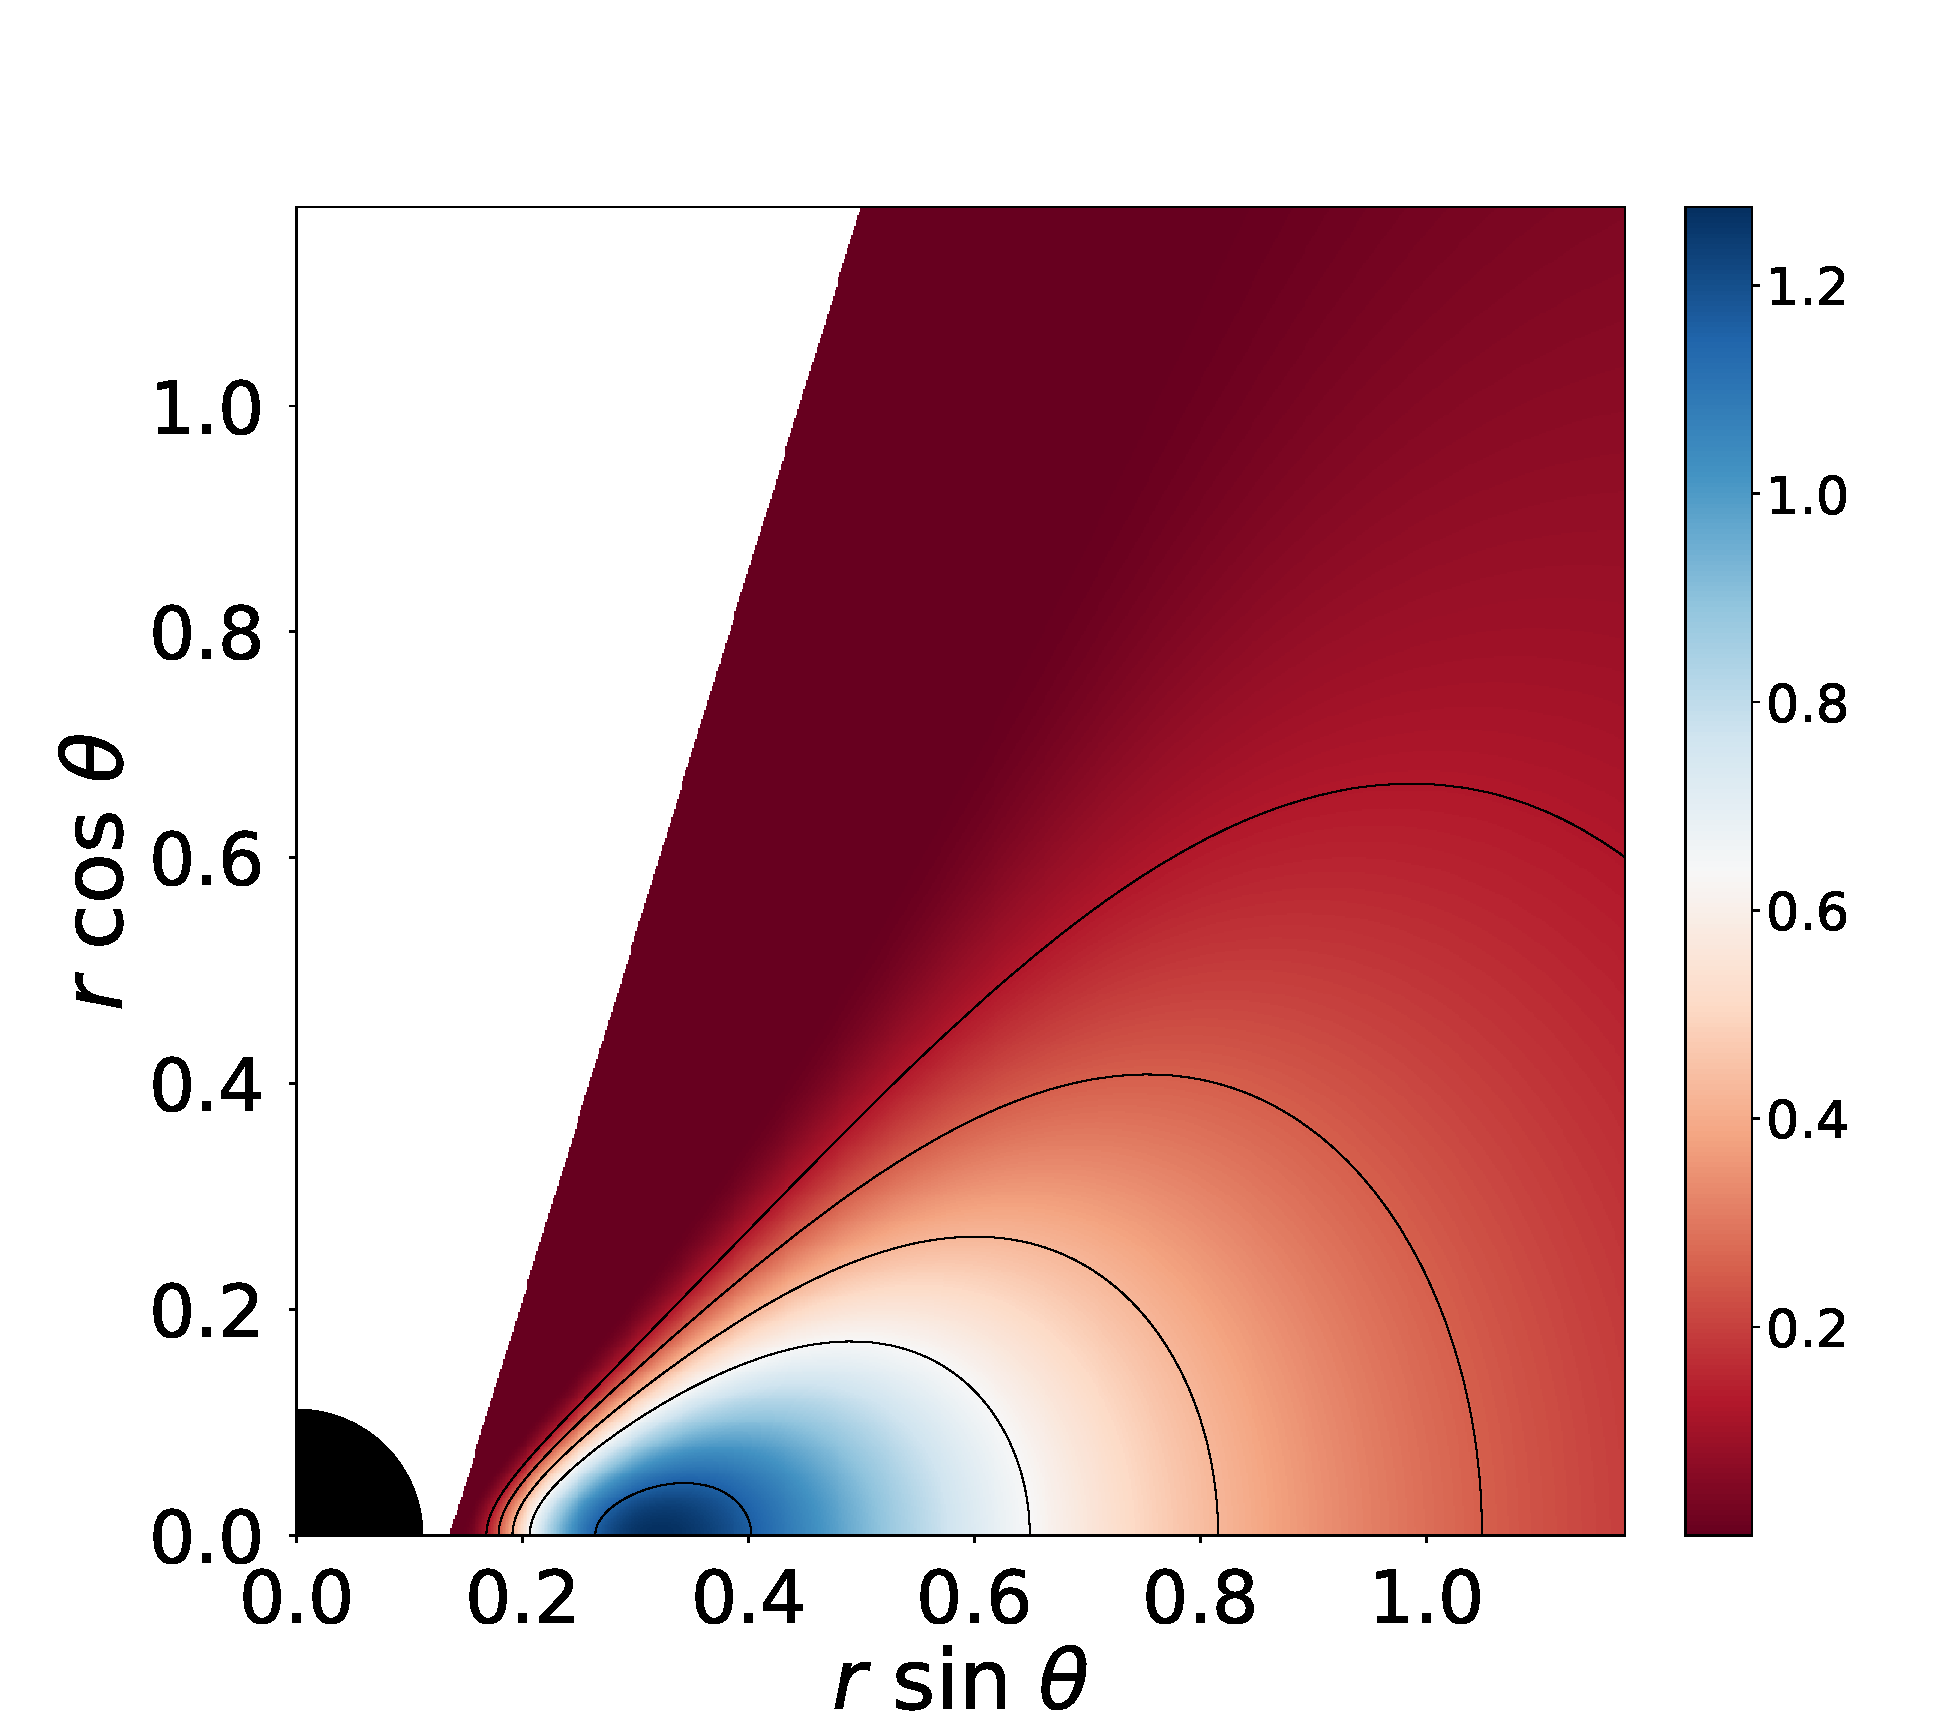
\includegraphics[scale=0.14]{figures/fig1_III_1.pdf}
\hspace{-0.2cm}
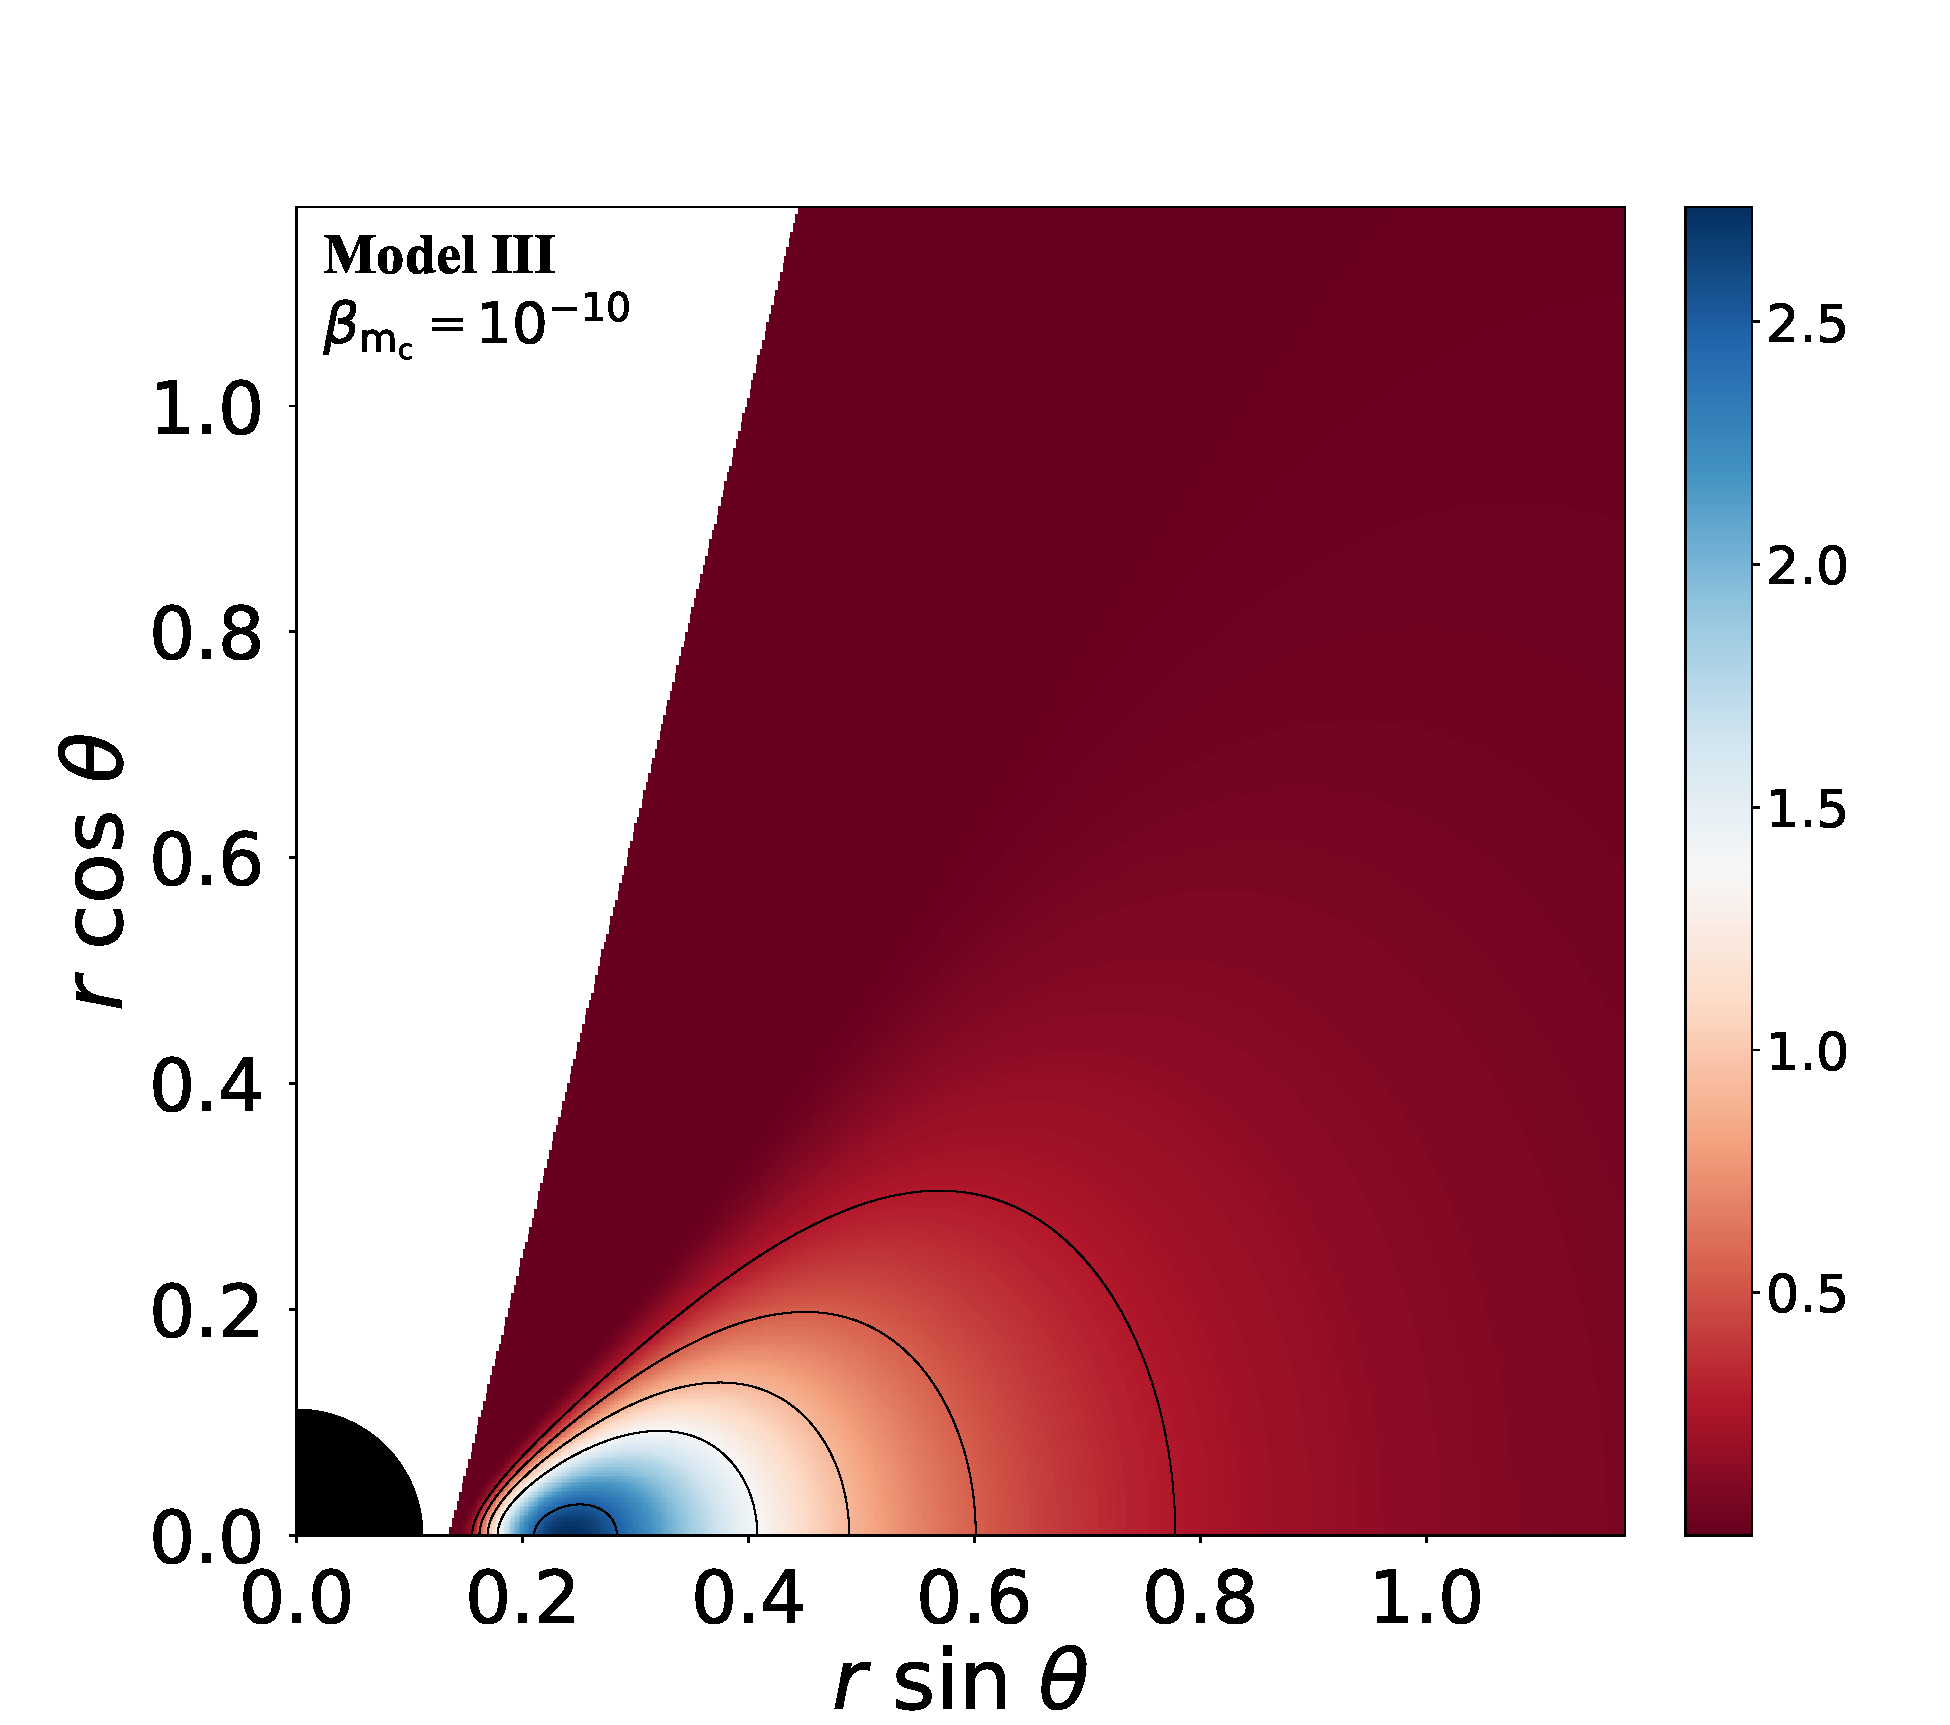
\includegraphics[scale=0.14]{figures/fig1_III__10.pdf}
\\
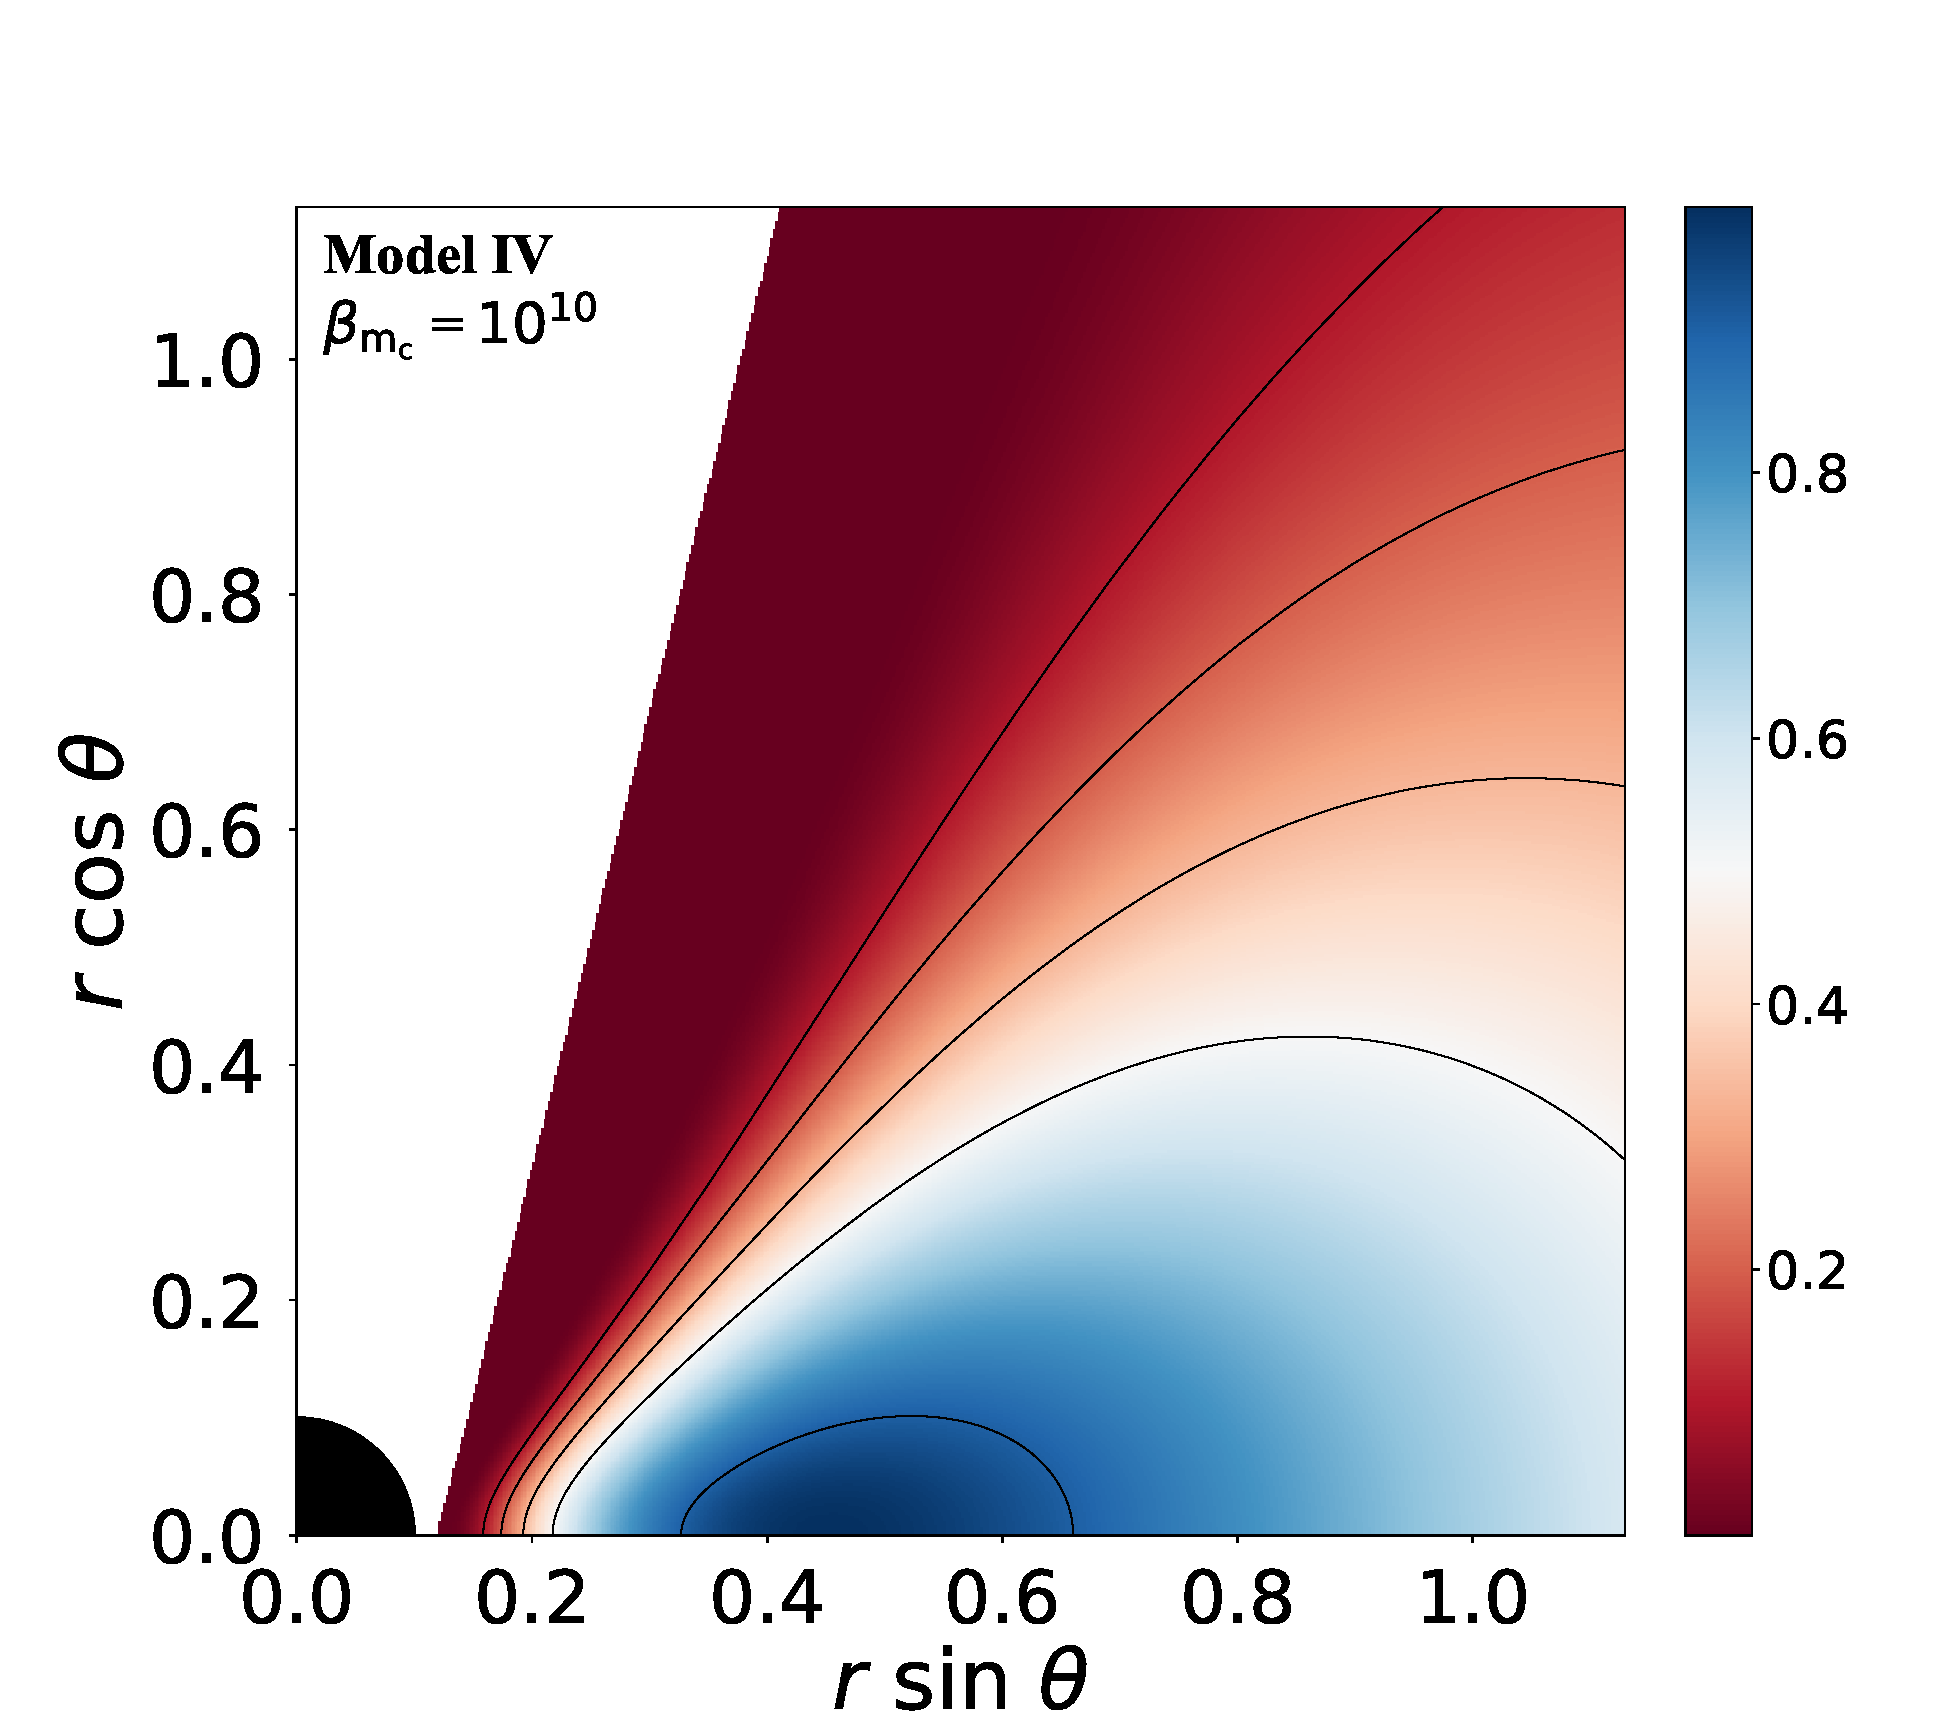
\includegraphics[scale=0.14]{figures/fig1_IV_10.pdf}
\hspace{-0.3cm}
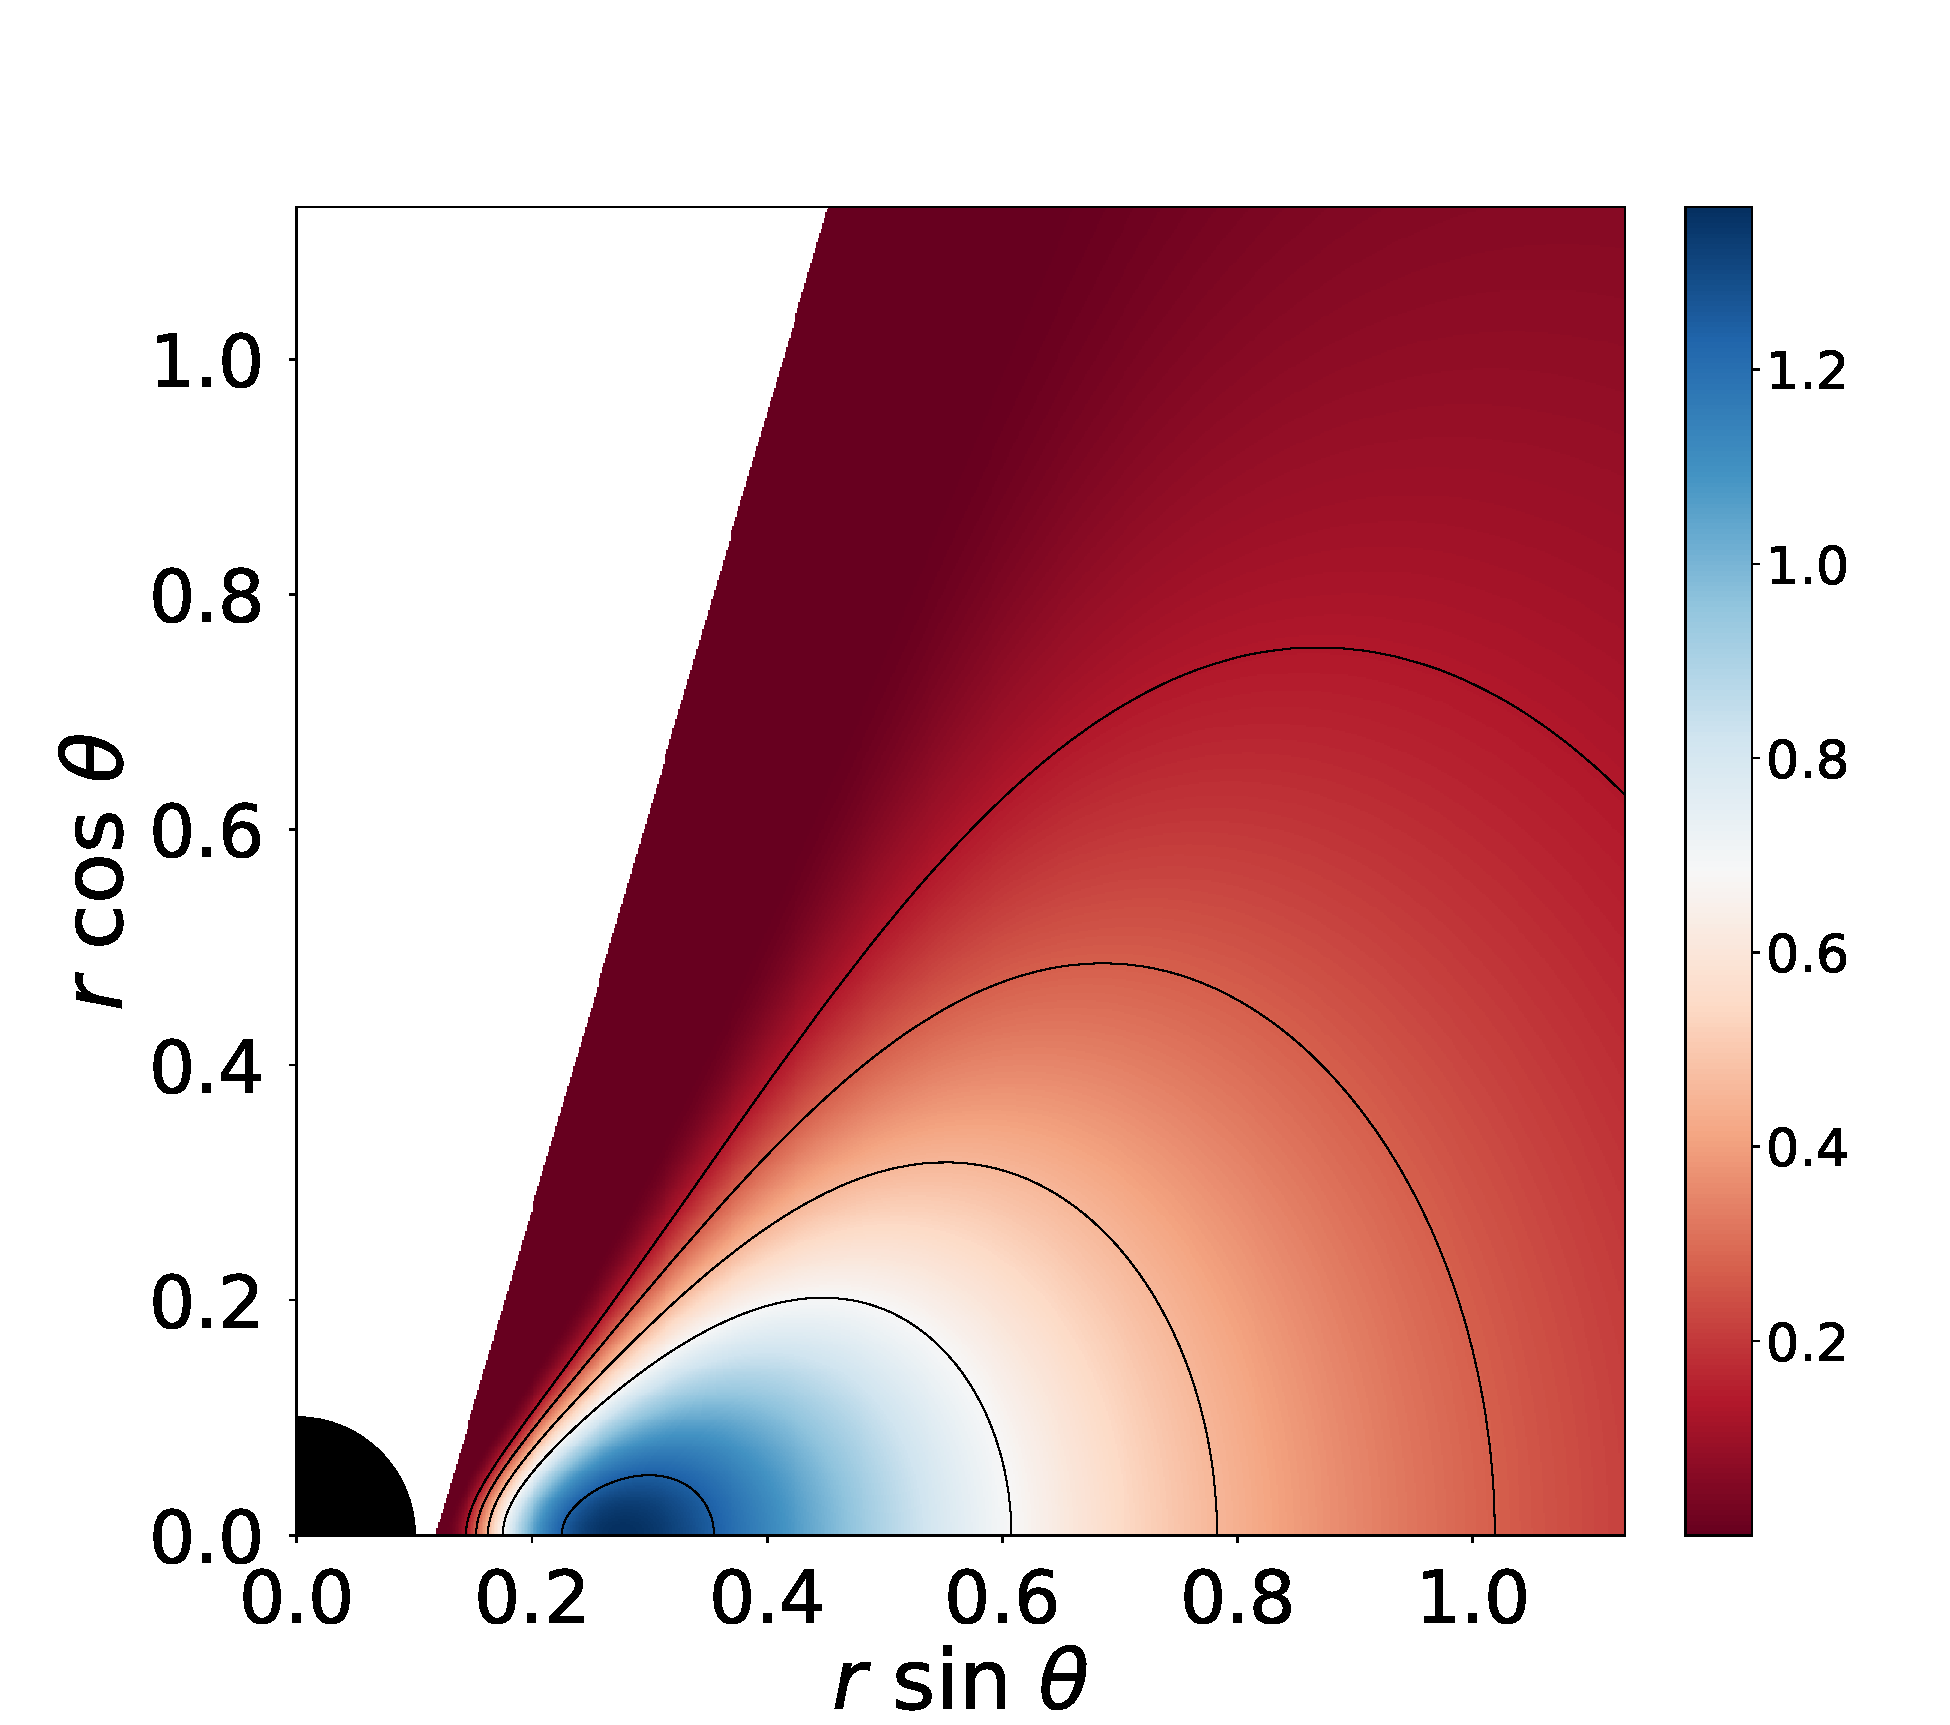
\includegraphics[scale=0.14]{figures/fig1_IV_1.pdf}
\hspace{-0.2cm}
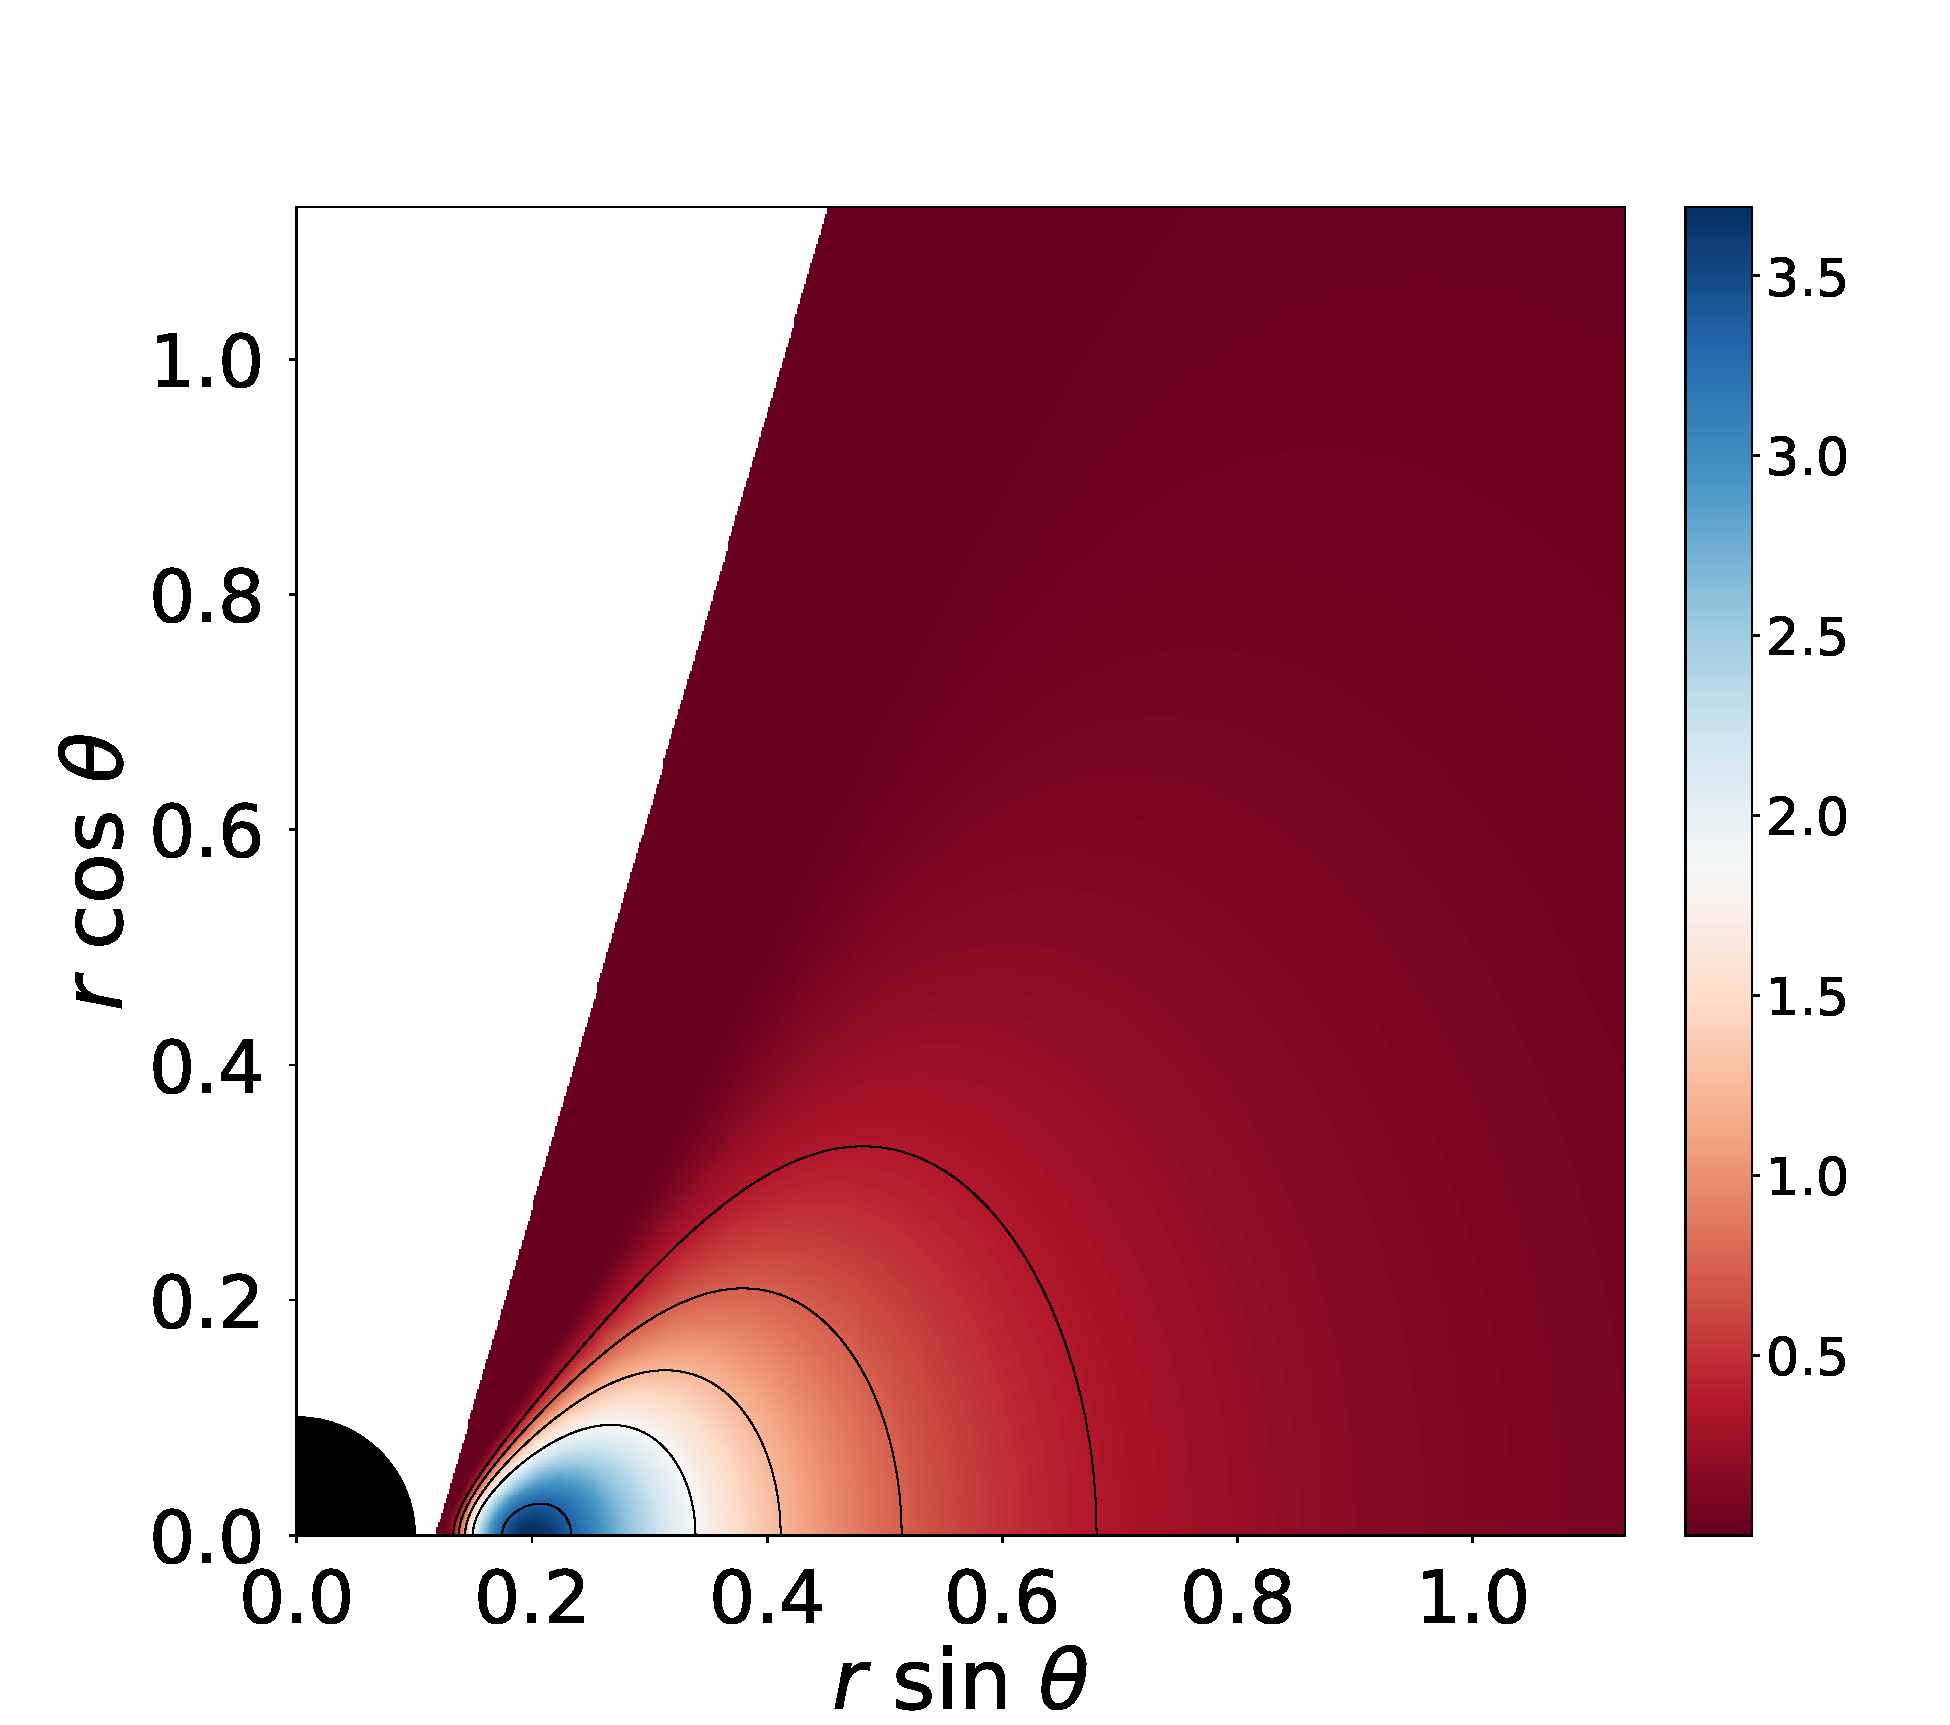
\includegraphics[scale=0.14]{figures/fig1_IV__10.pdf}
\hspace{-0.2cm}
\caption{Rest-mass density distribution. From top to bottom the rows correspond to the different models for the KBHsSH (I, II, III and IV). From left to right the columns correspond to different values of the magnetization parameter, namely non-magnetized ($\beta_{\mathrm{m}_{\mathrm{c}}} = 10^{10}$), mildly magnetized ($\beta_{\mathrm{m}_{\mathrm{c}}} = 1$) and strongly magnetized ($\beta_{\mathrm{m}_{\mathrm{c}}} = 10^{-10}$)}
\label{models_I}
\end{figure*}

\begin{figure*}
\centering
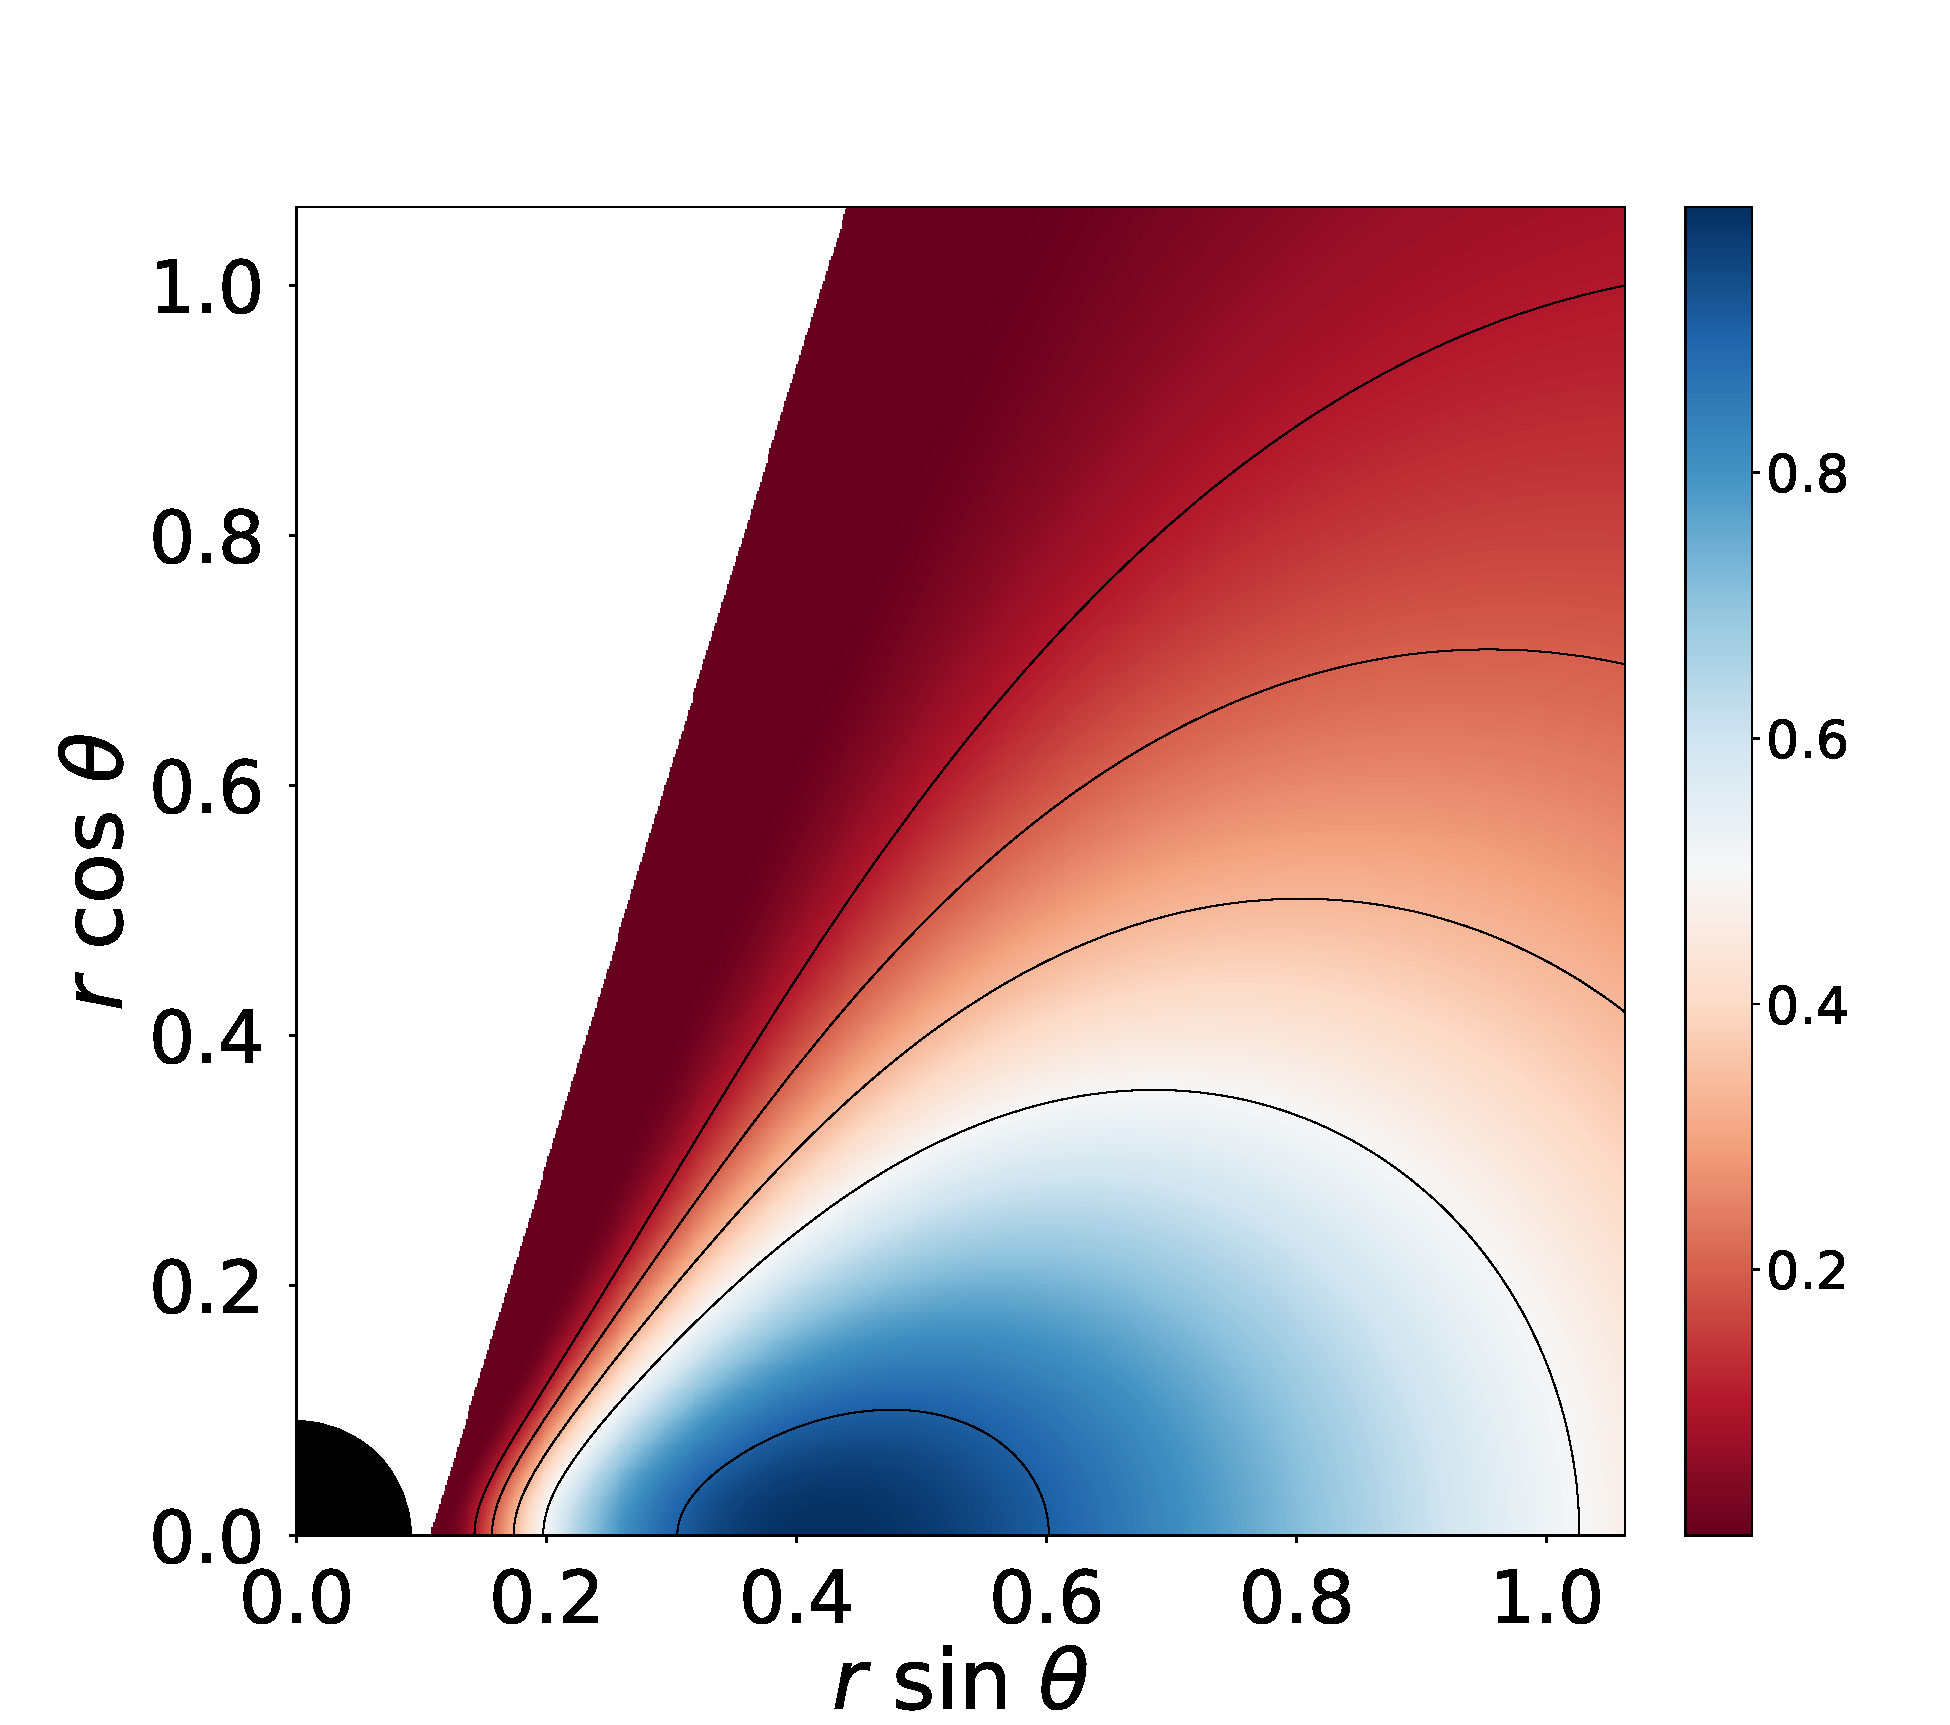
\includegraphics[scale=0.14]{figures/fig2_V_10.pdf}
\hspace{-0.3cm}
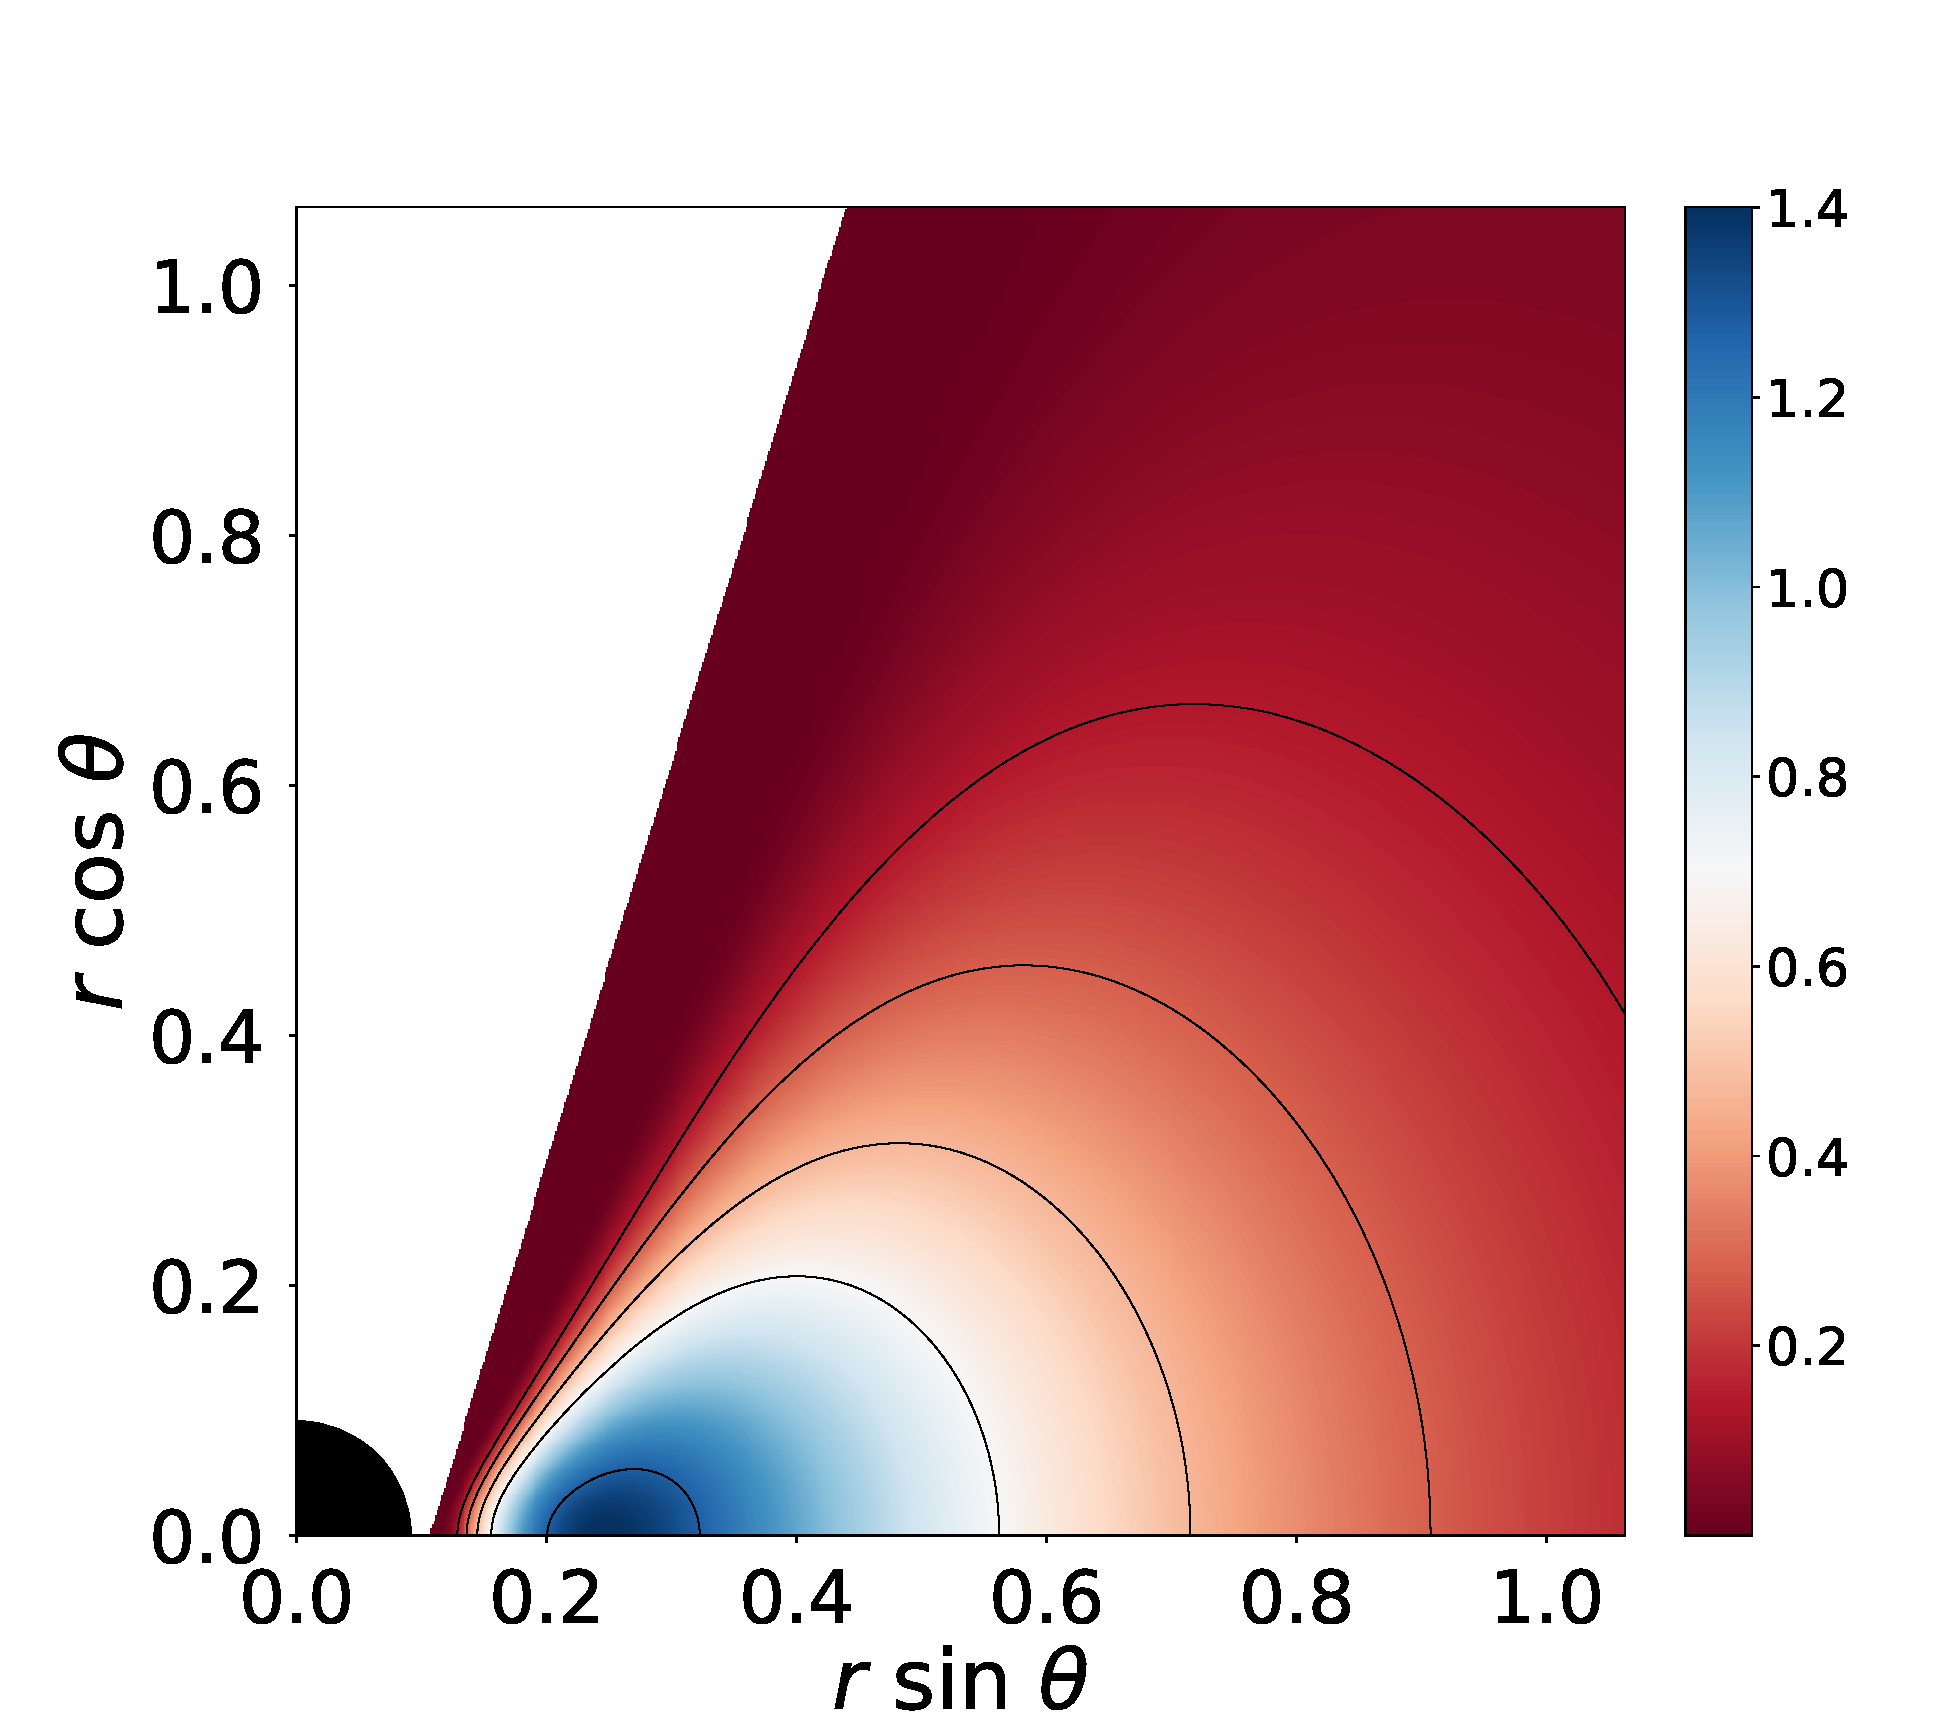
\includegraphics[scale=0.14]{figures/fig2_V_1.pdf}
\hspace{-0.2cm}
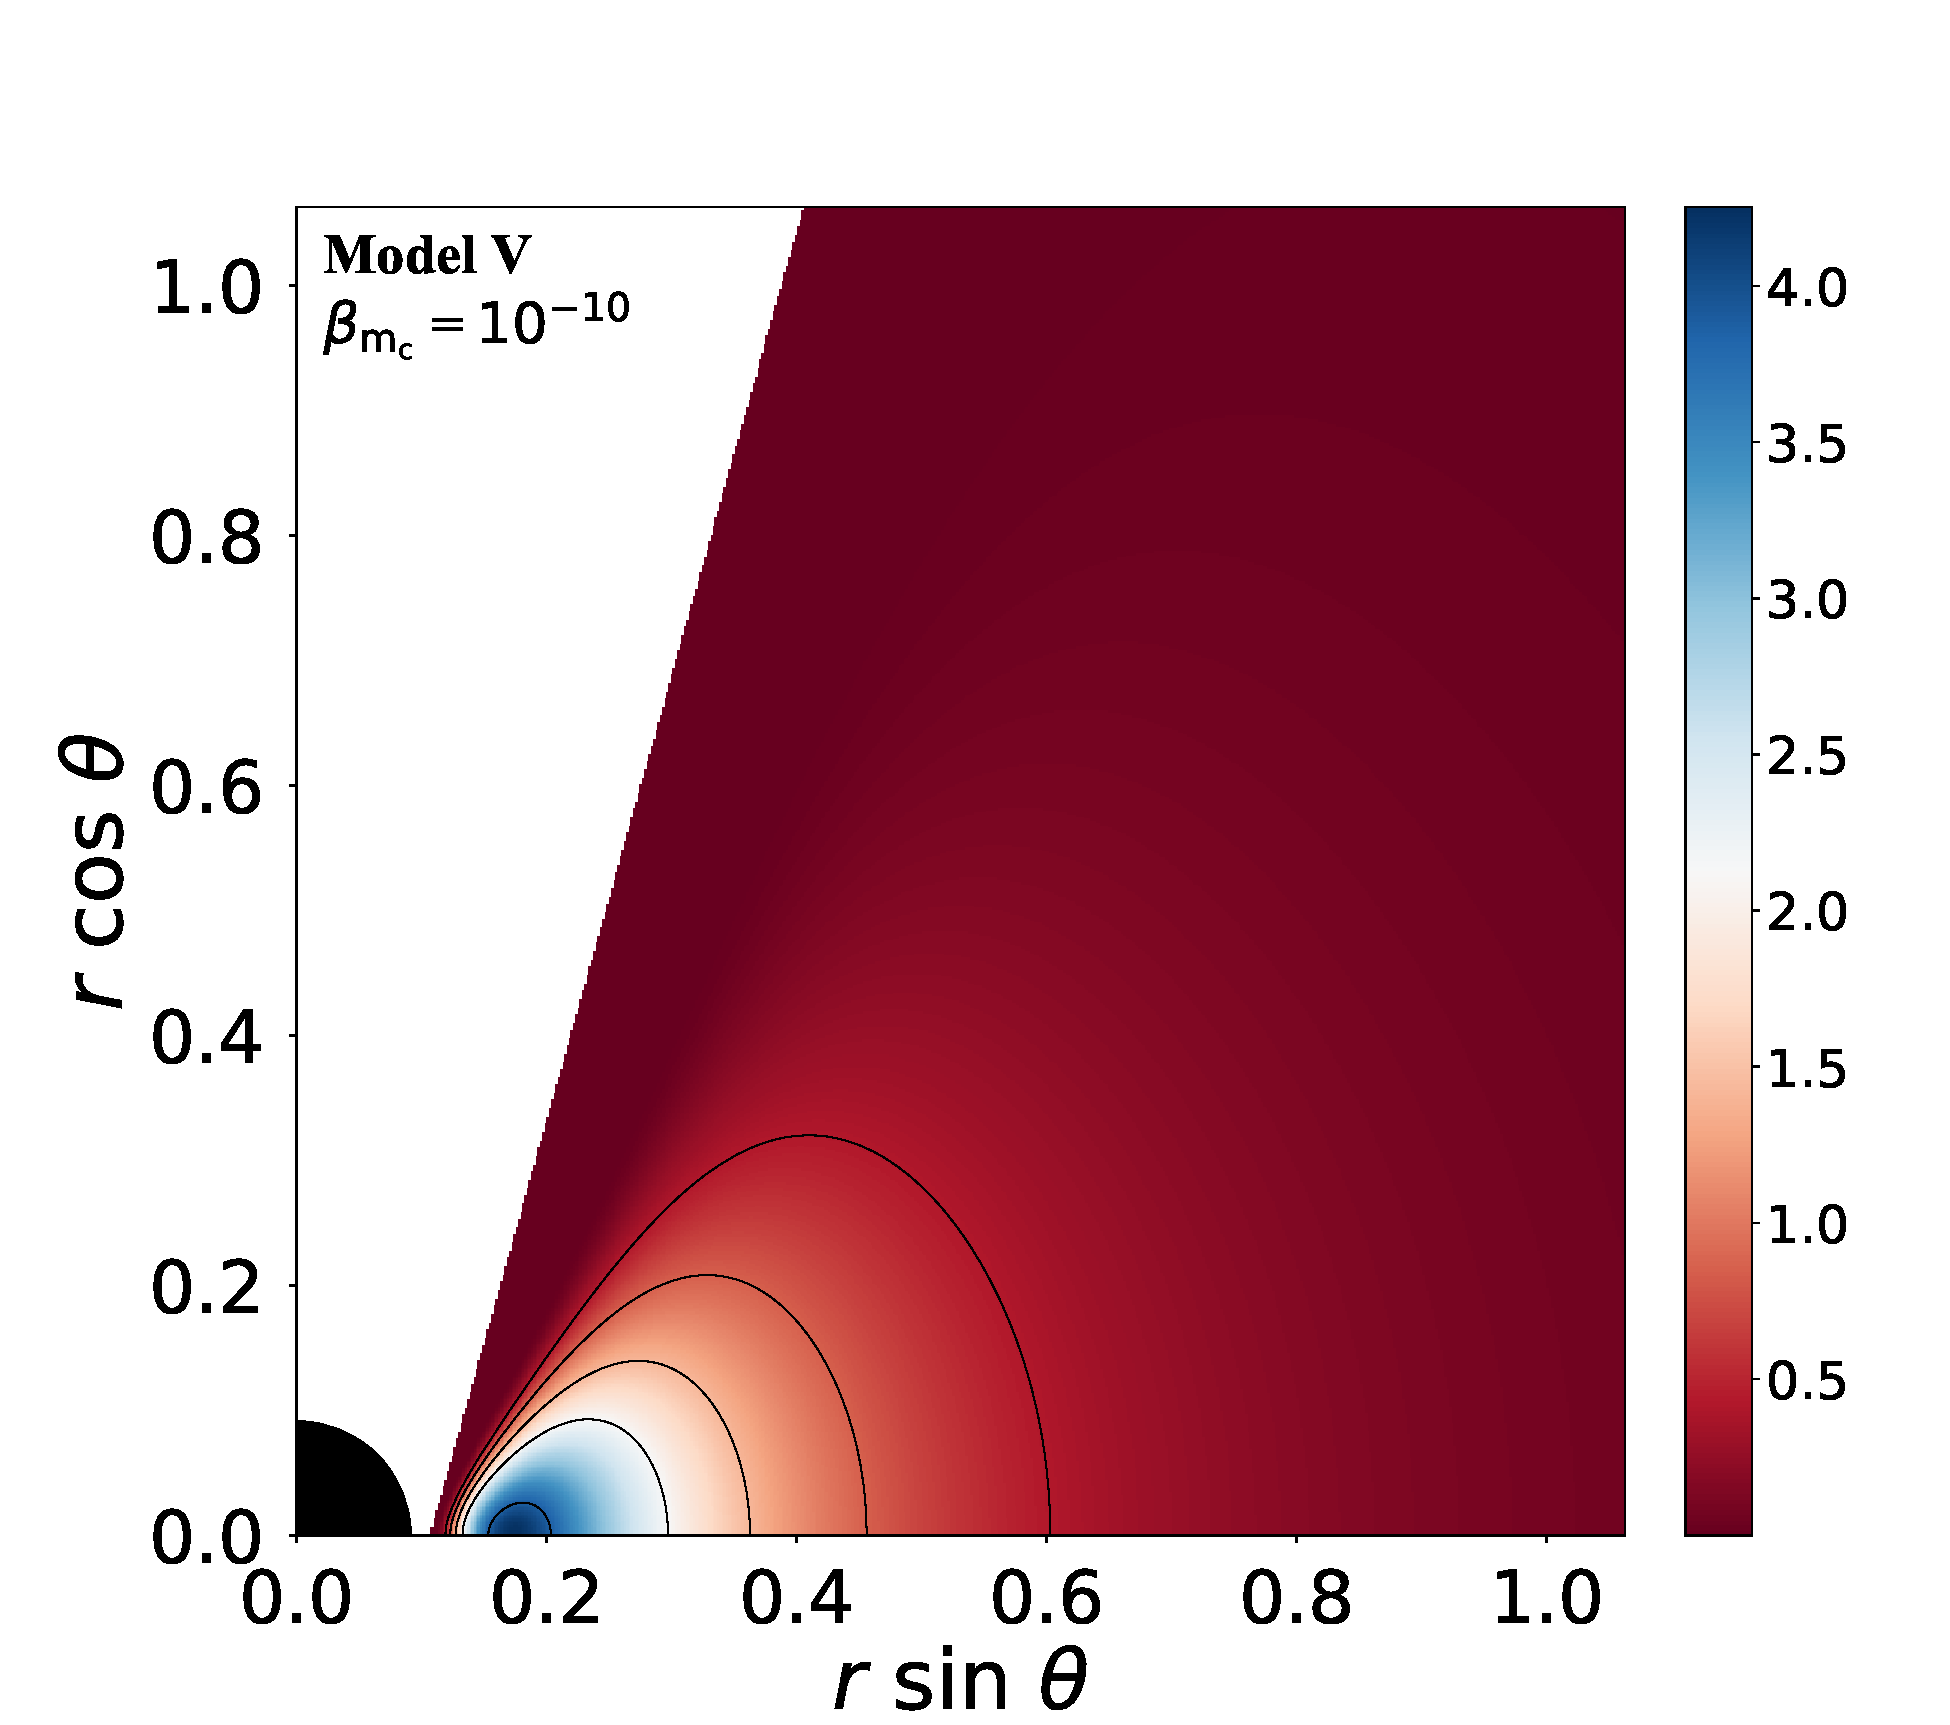
\includegraphics[scale=0.14]{figures/fig2_V__10.pdf}
\\
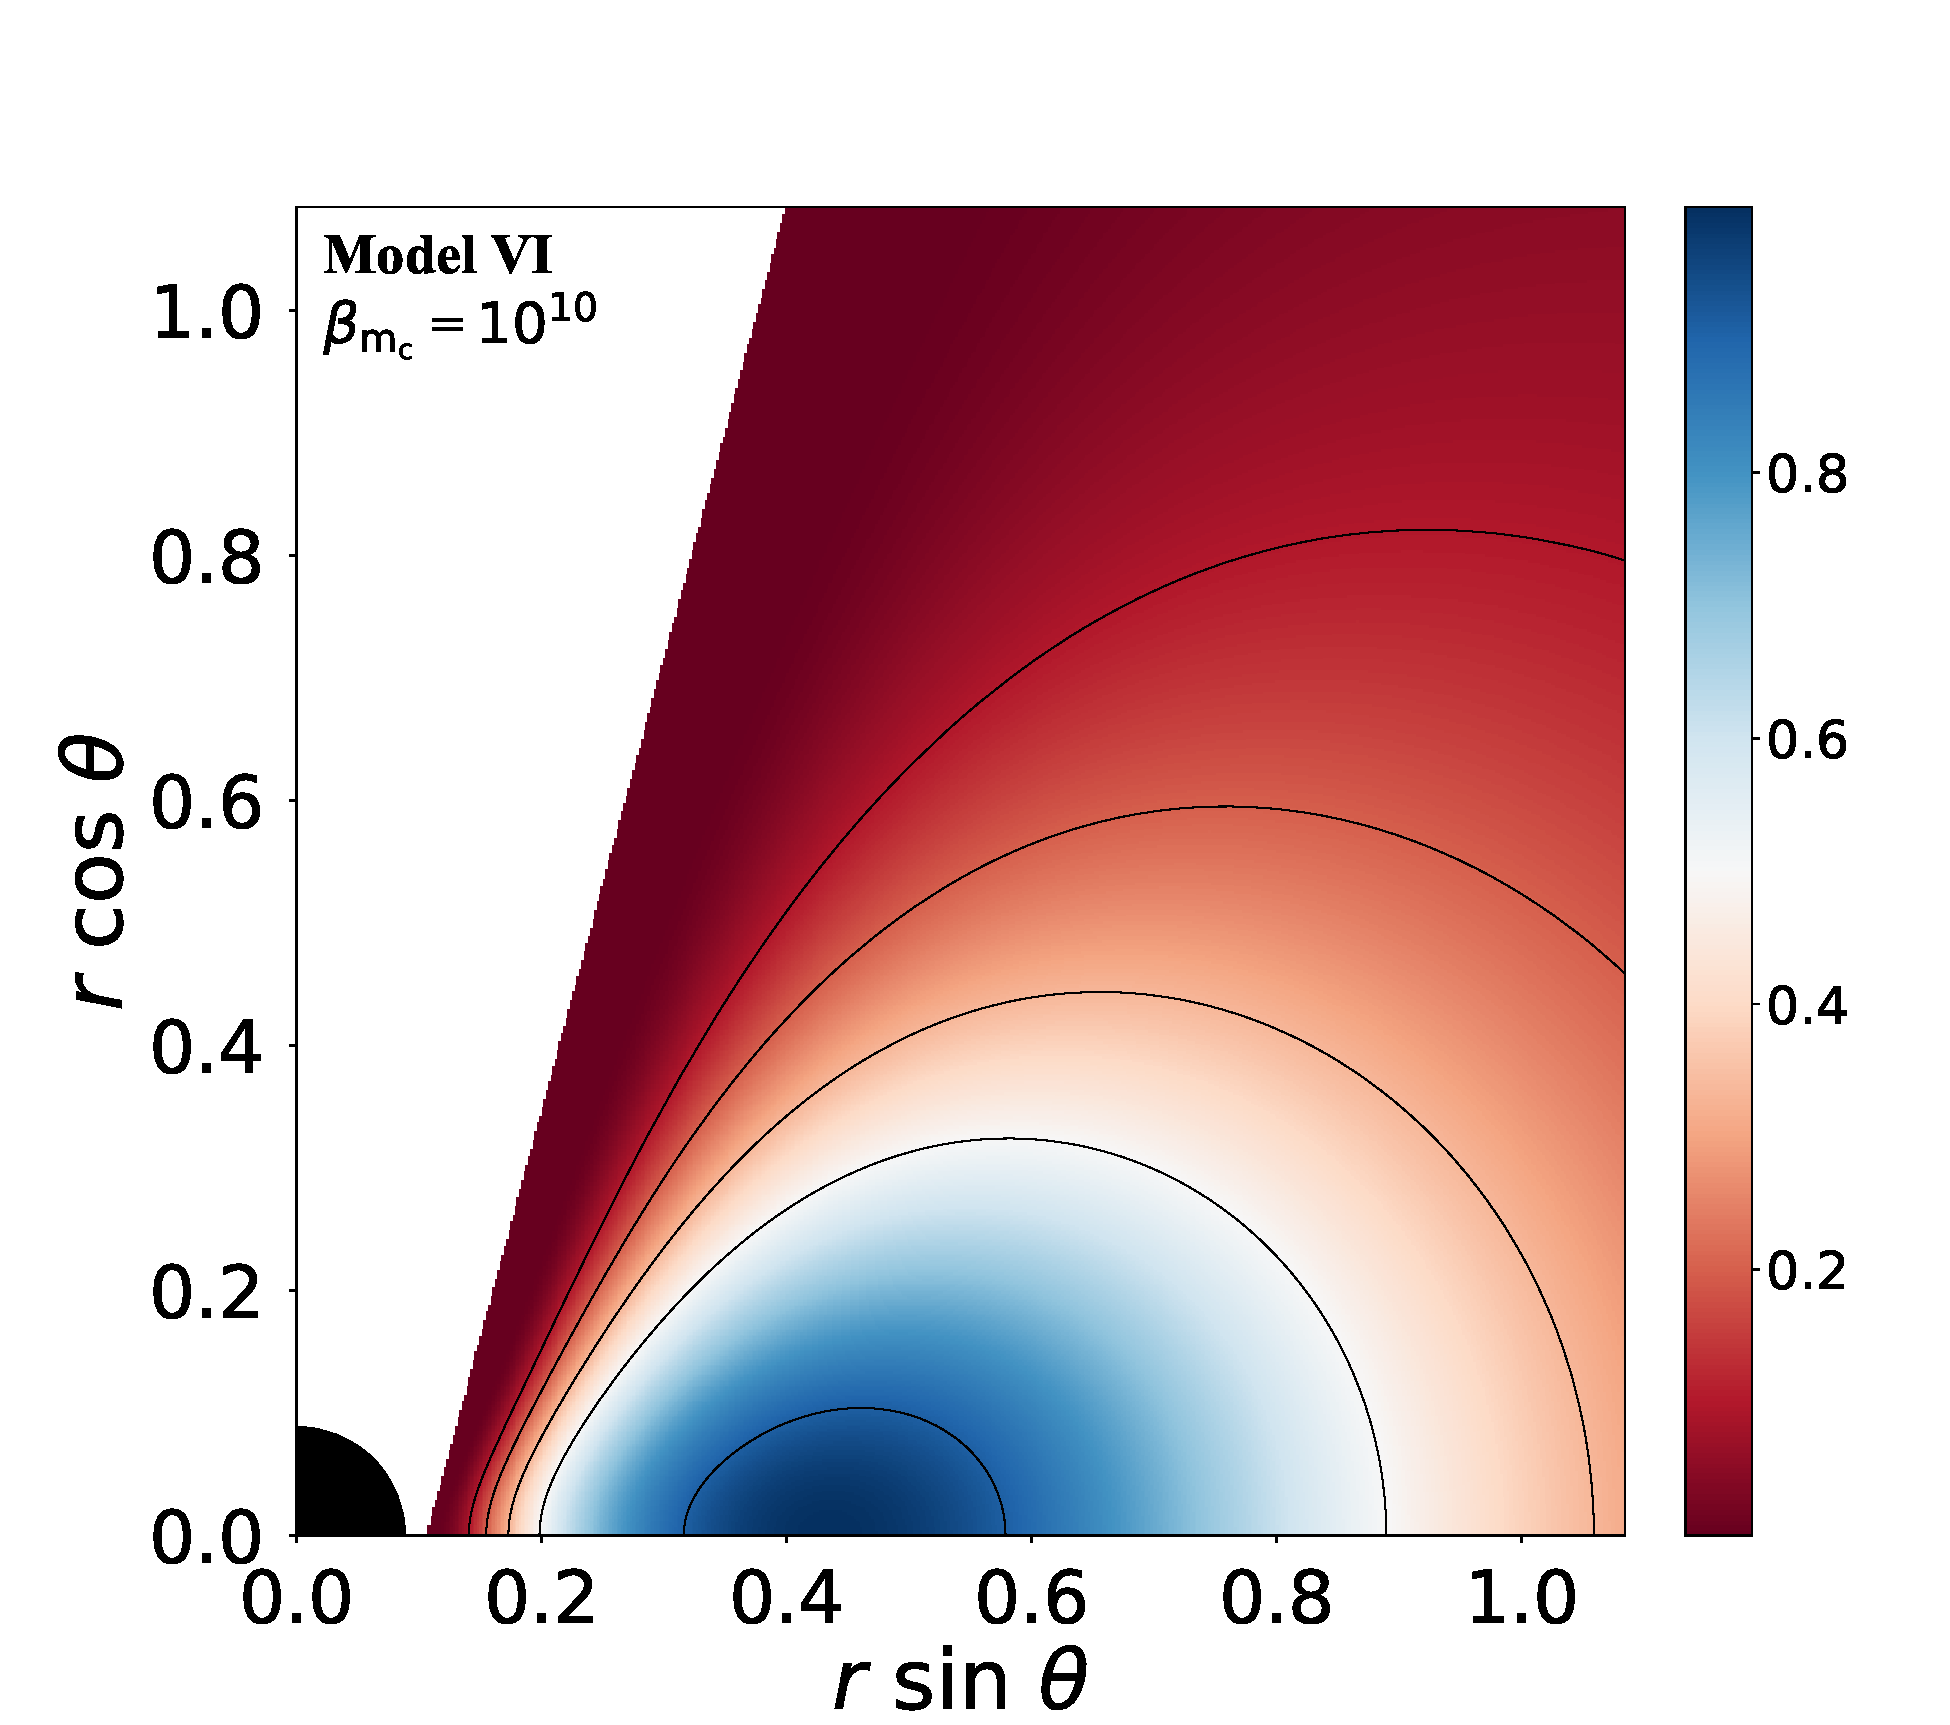
\includegraphics[scale=0.14]{figures/fig2_VI_10.pdf}
\hspace{-0.3cm}
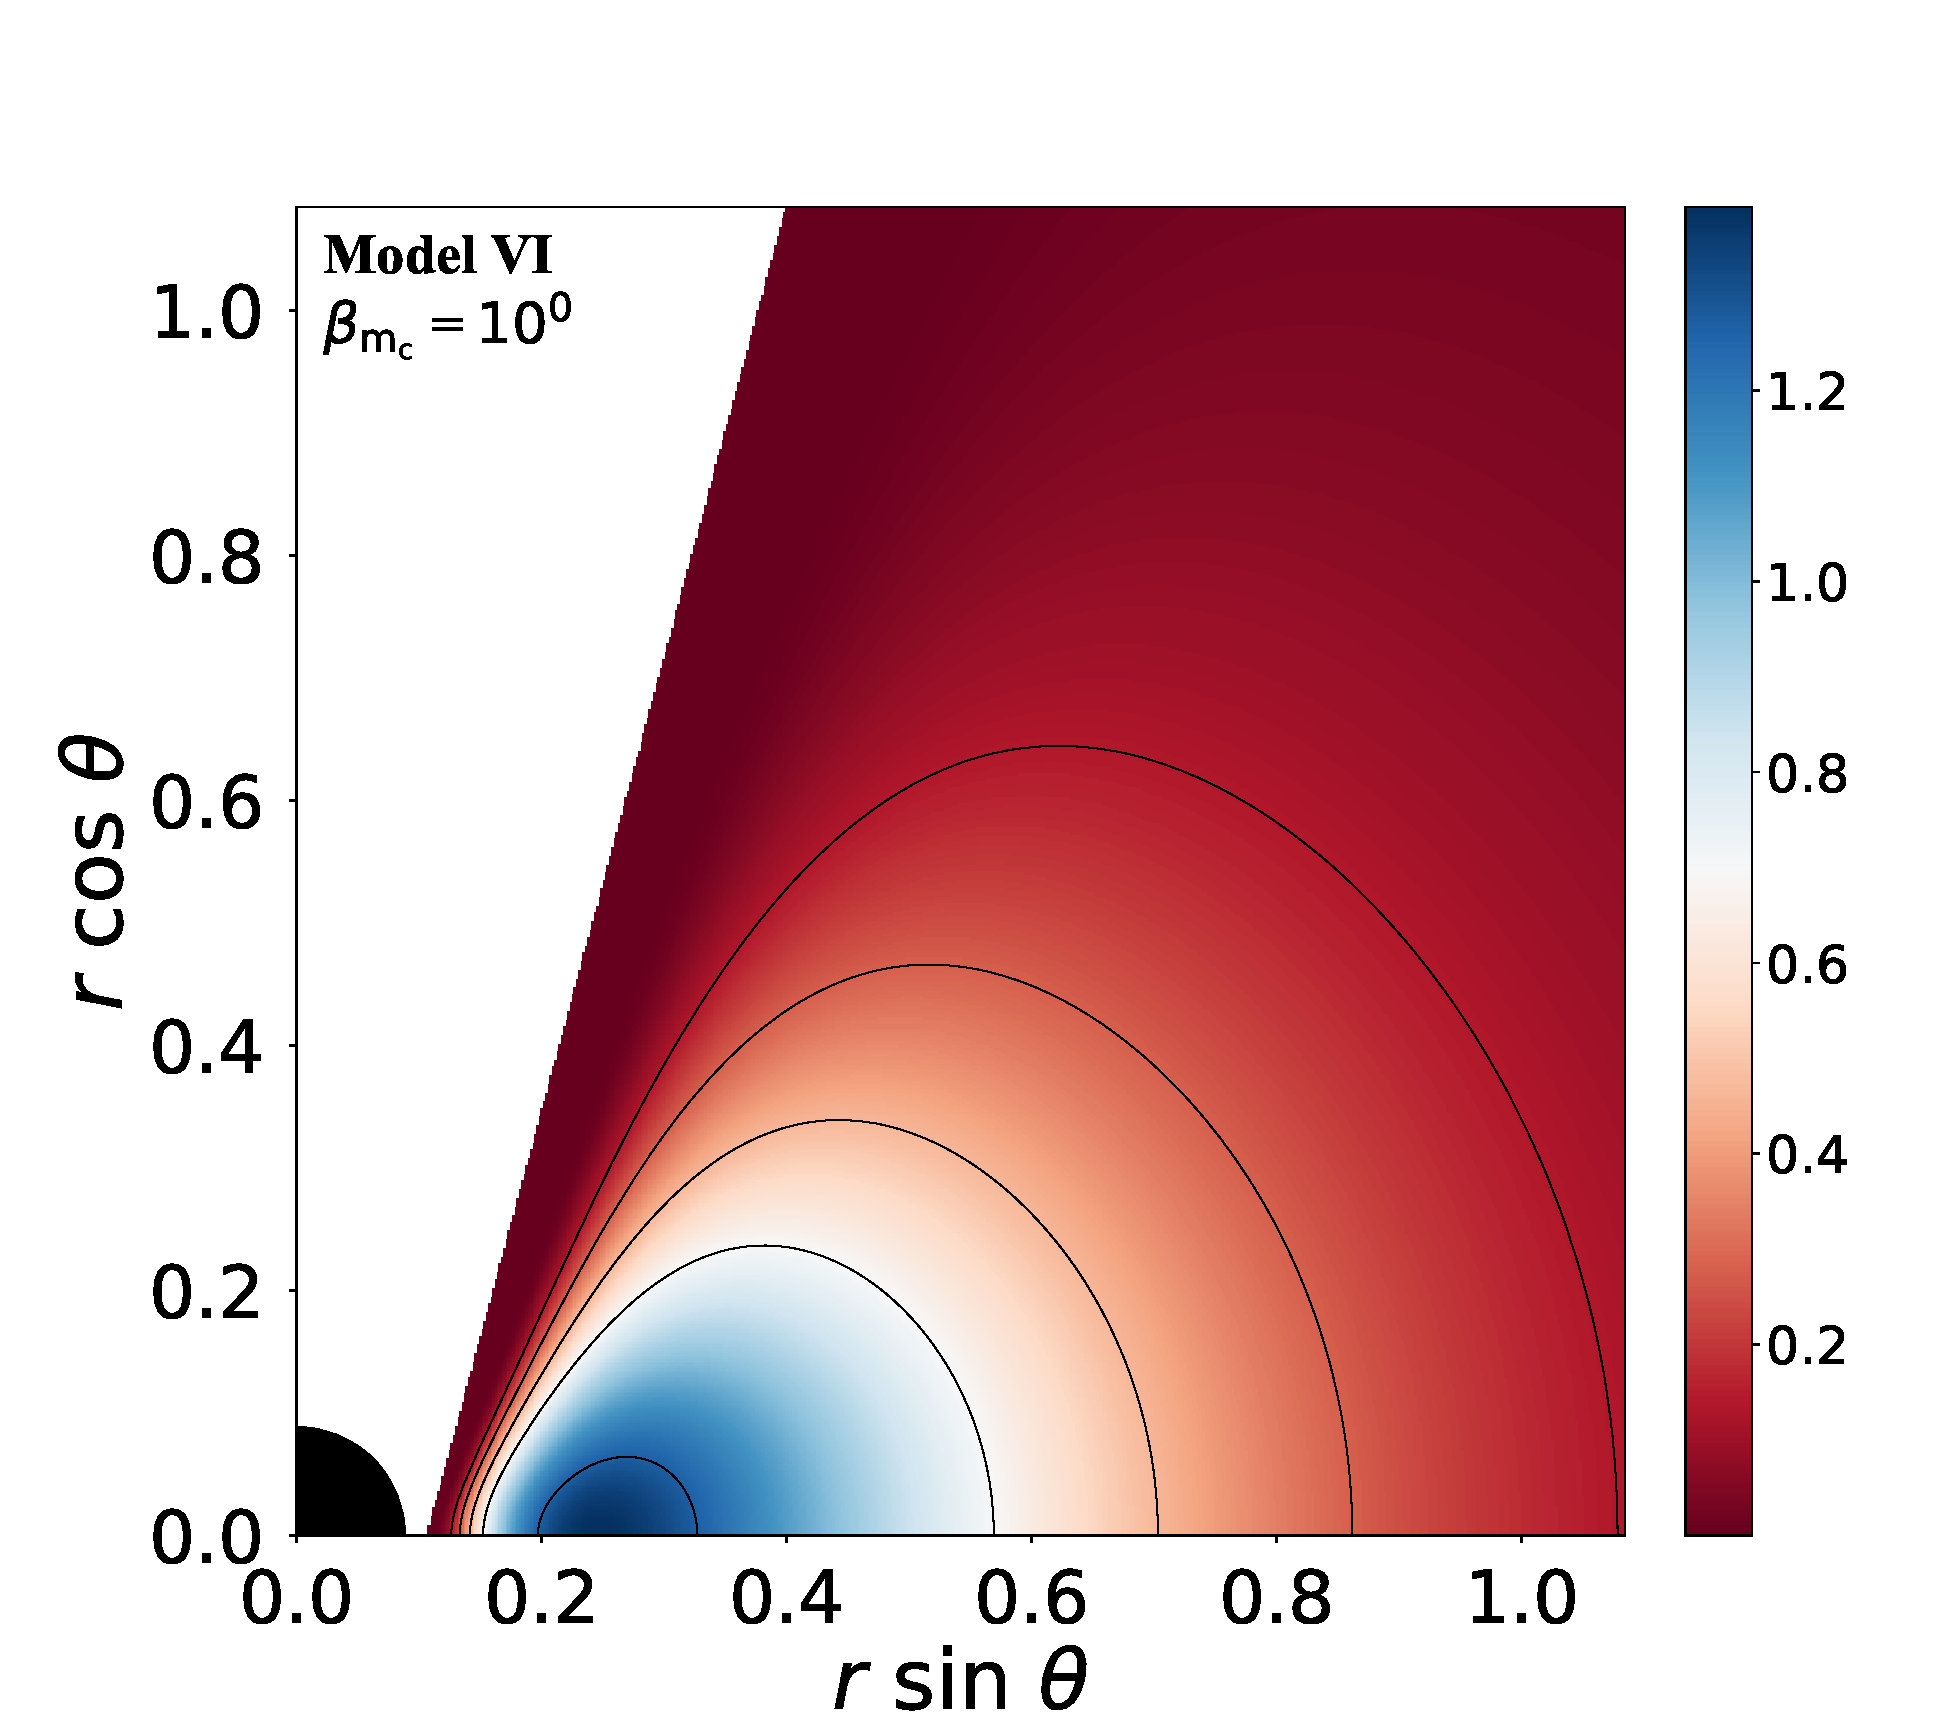
\includegraphics[scale=0.14]{figures/fig2_VI_1.pdf}
\hspace{-0.2cm}
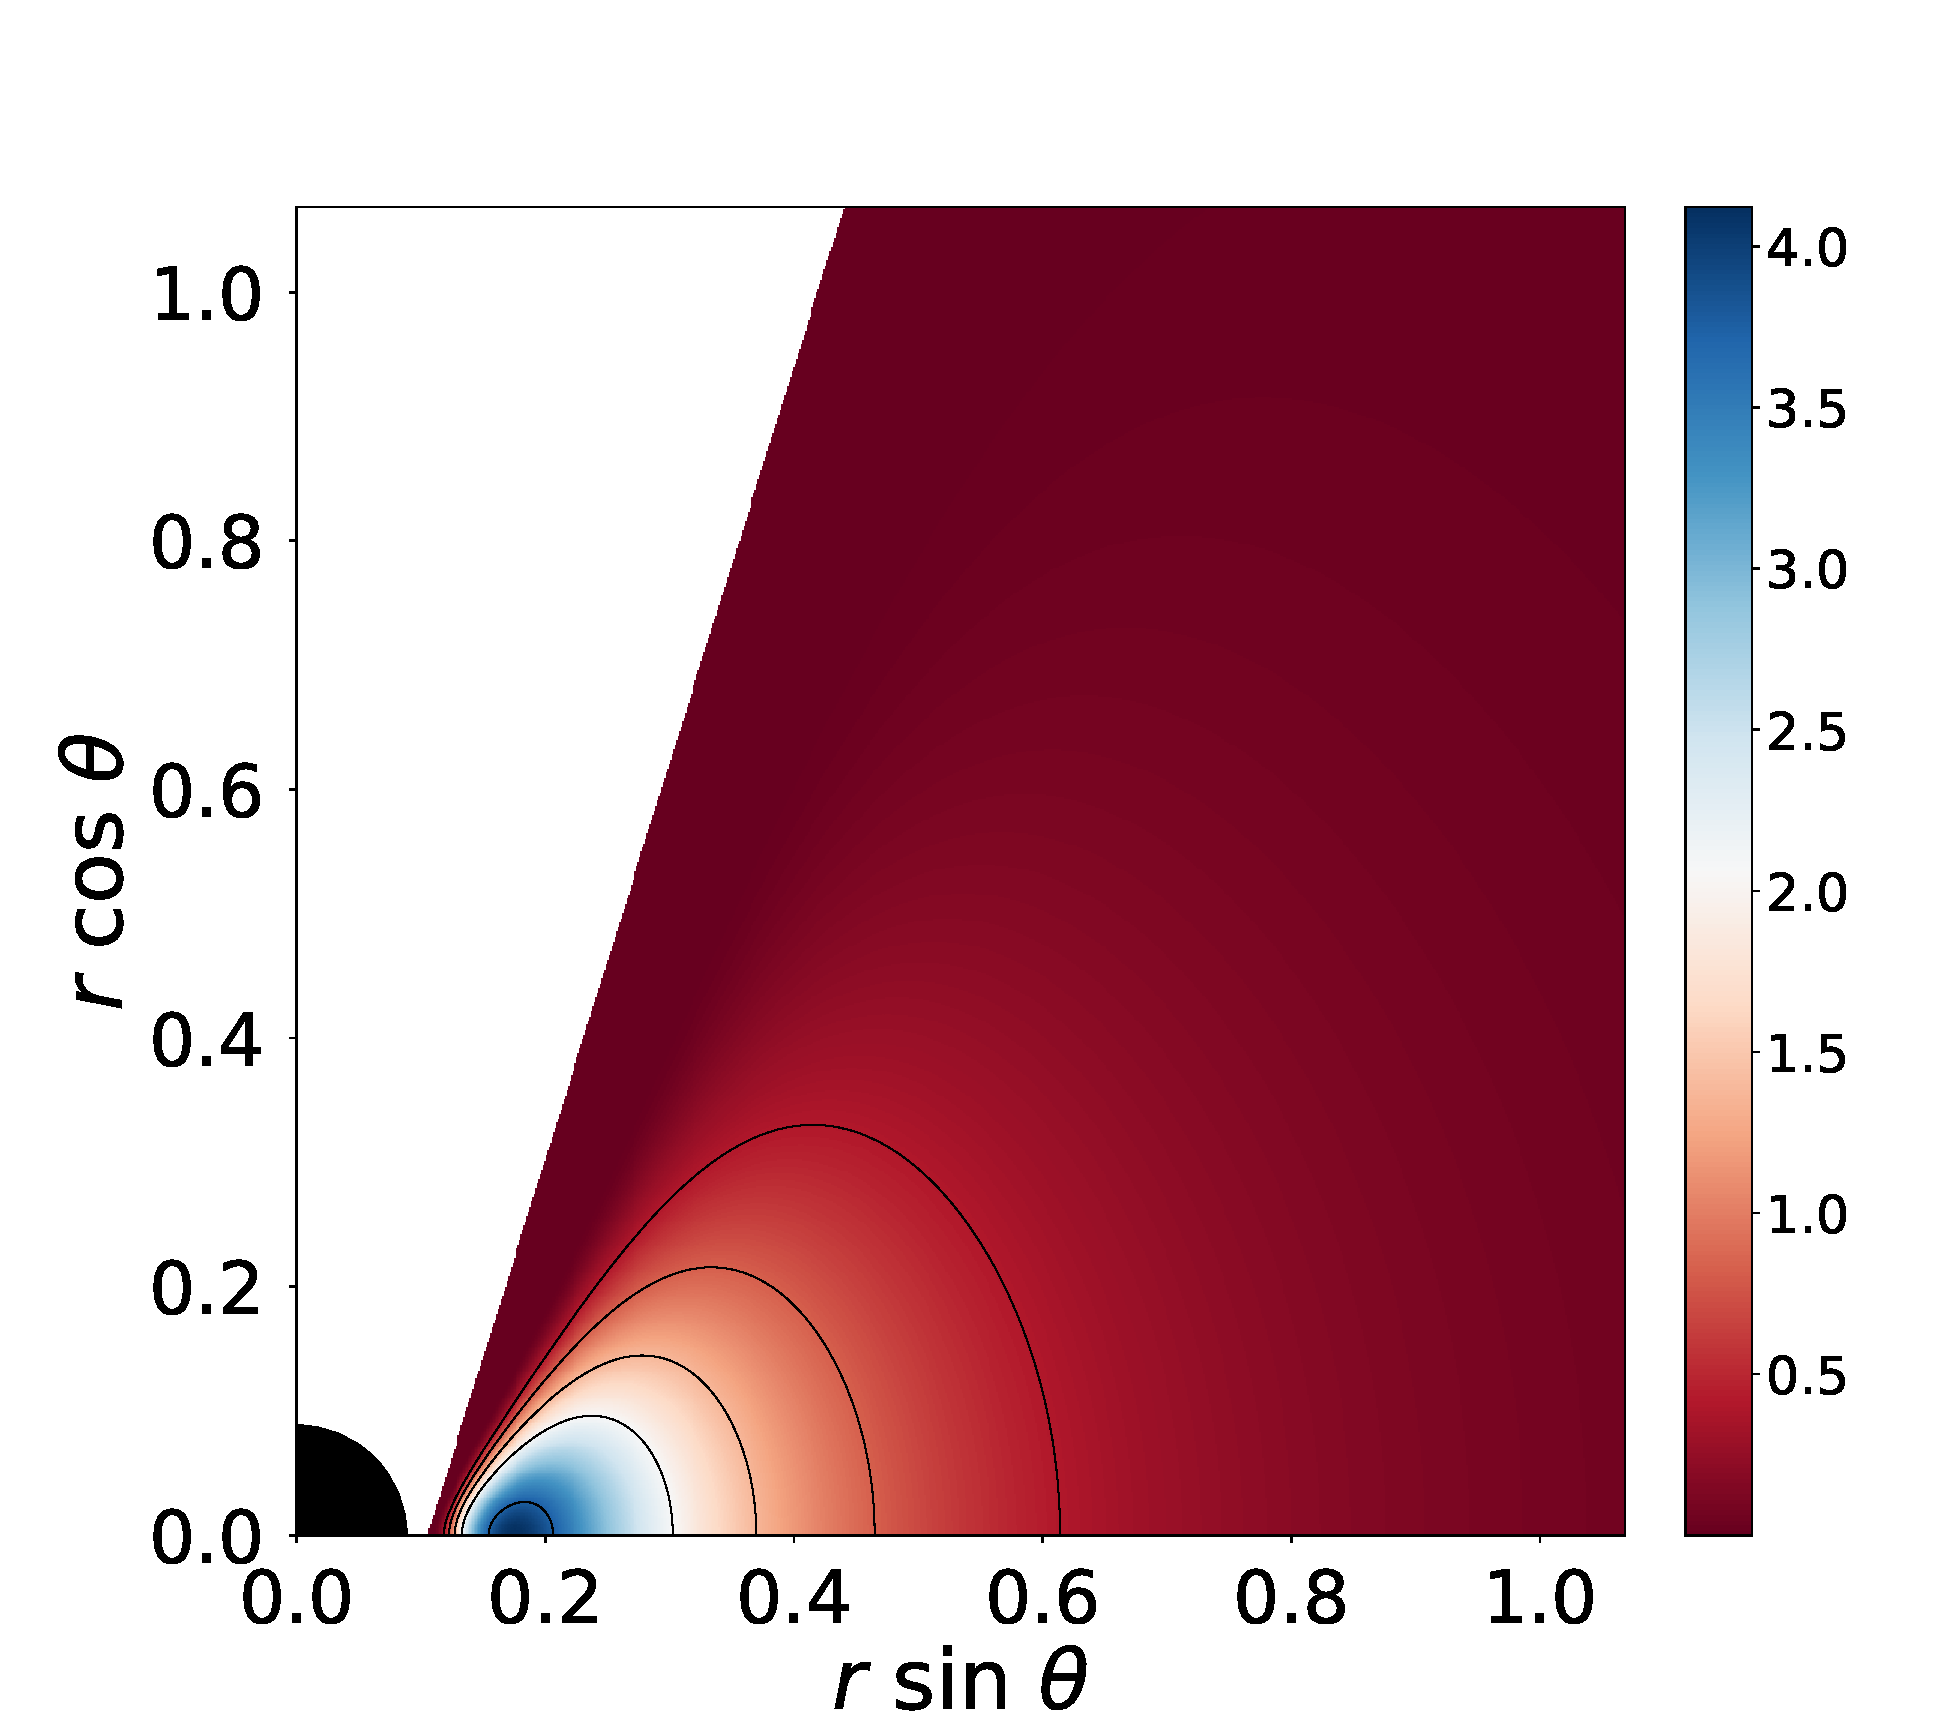
\includegraphics[scale=0.14]{figures/fig2_VI__10.pdf}
\\
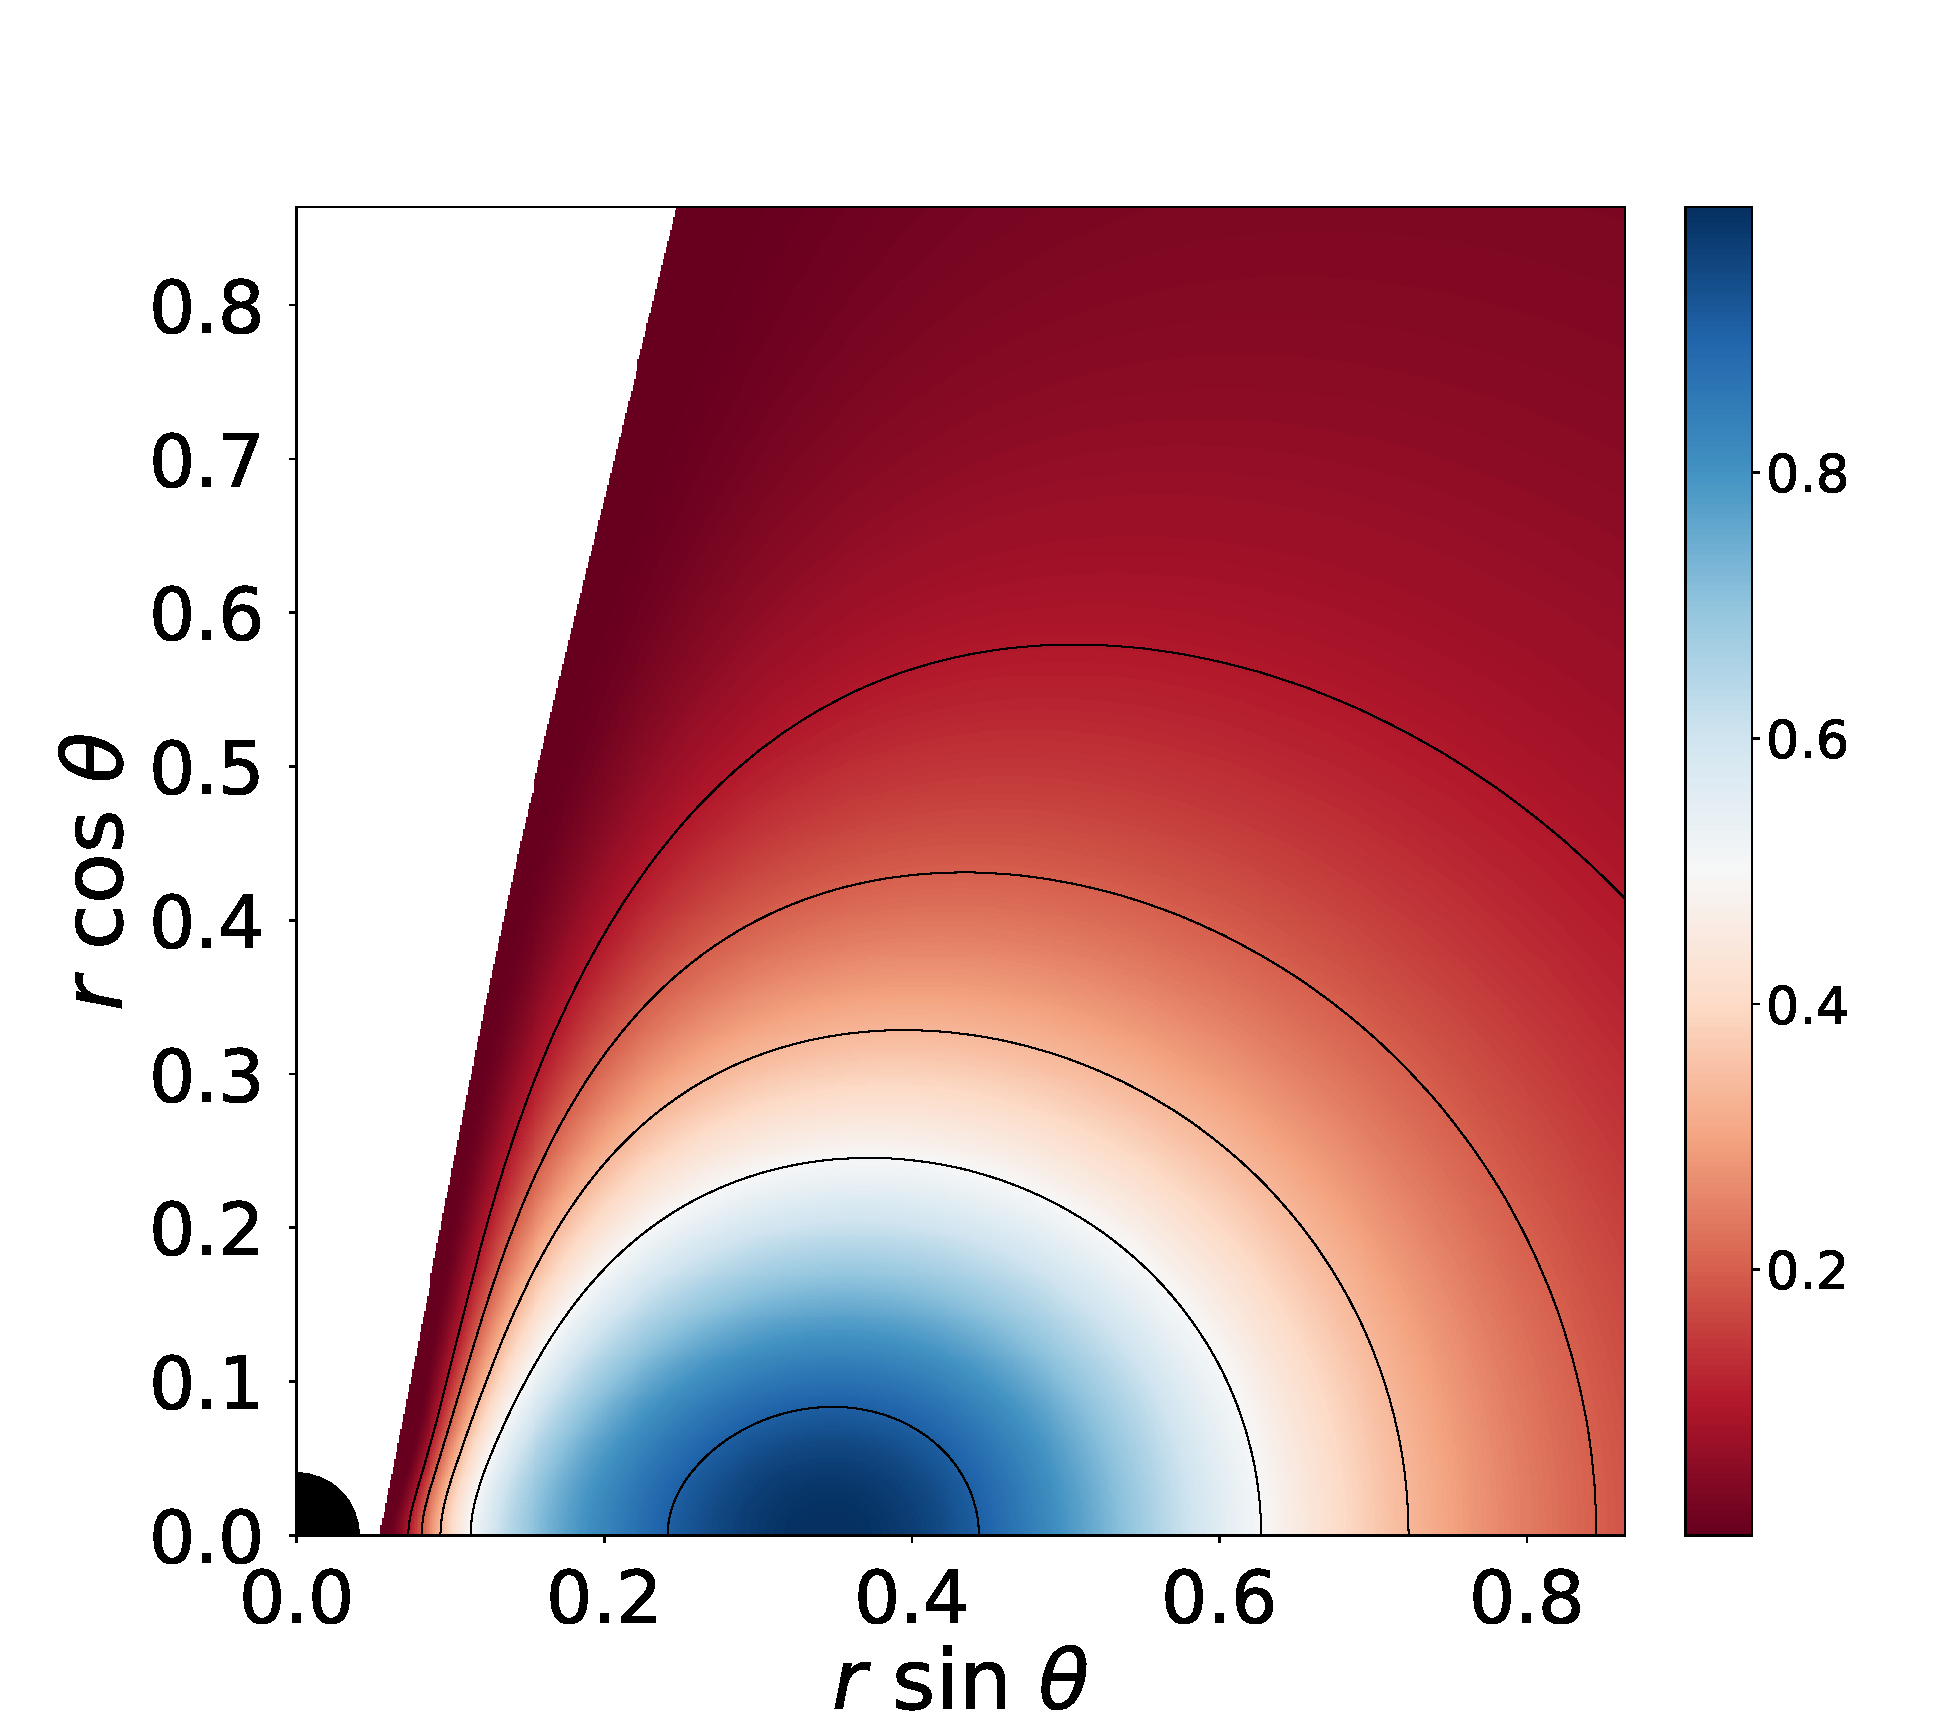
\includegraphics[scale=0.14]{figures/fig2_VII_10.pdf}
\hspace{-0.3cm}
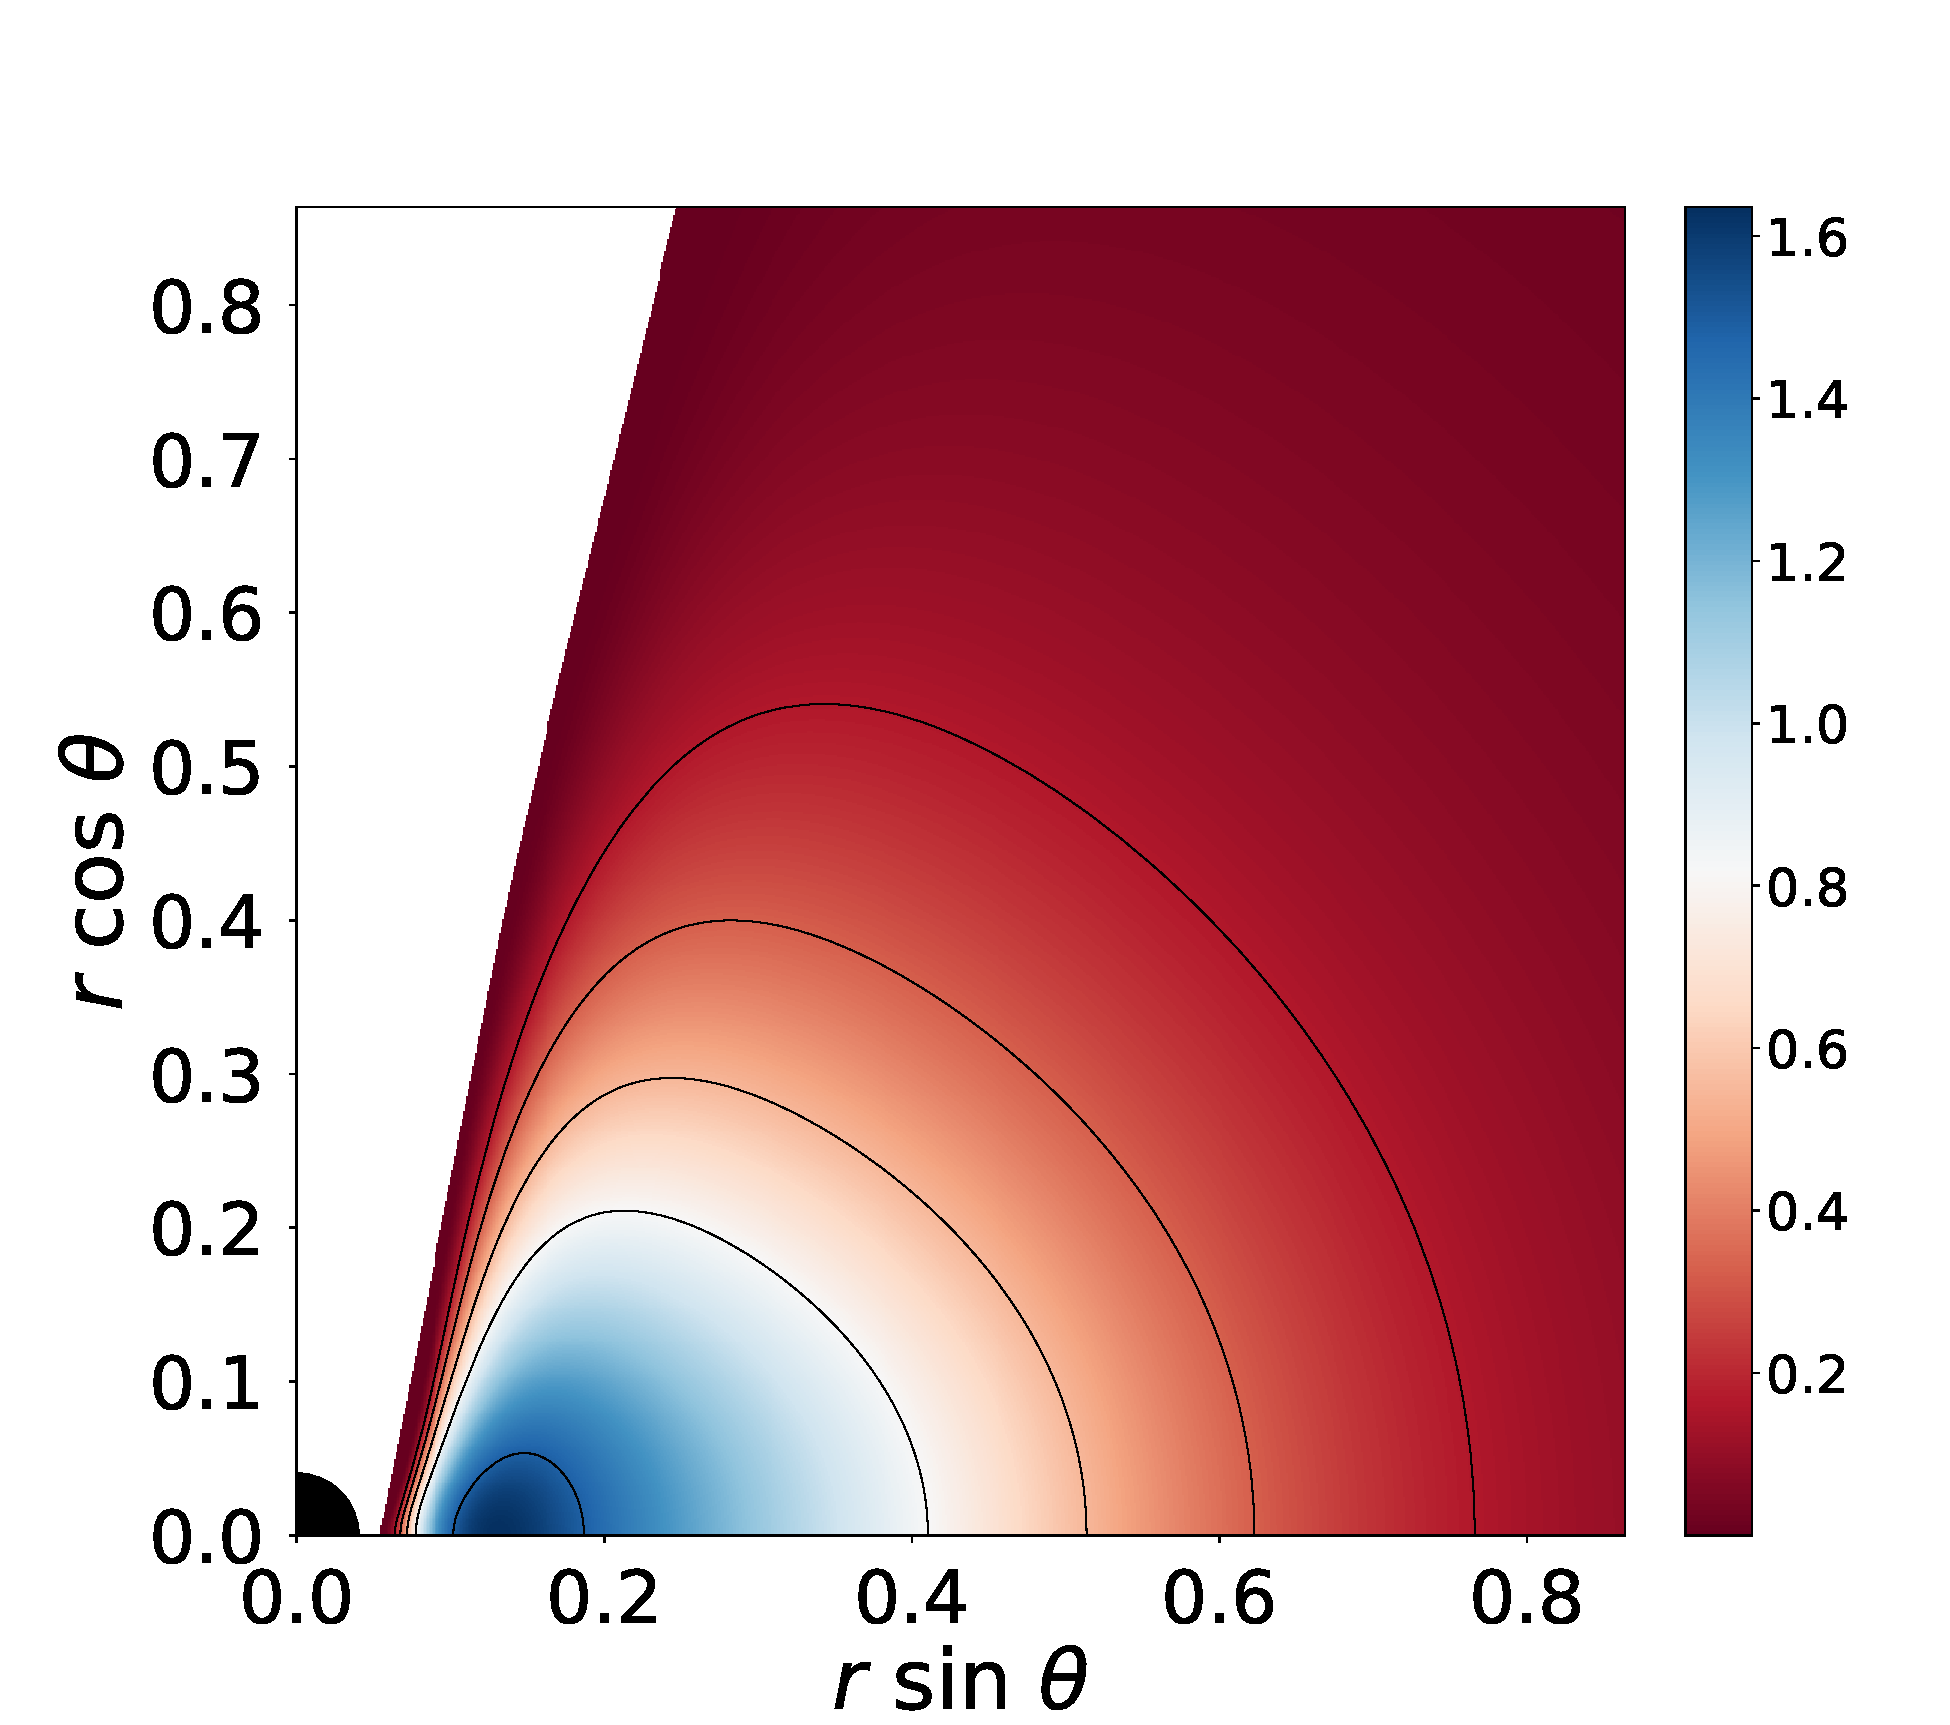
\includegraphics[scale=0.14]{figures/fig2_VII_1.pdf}
\hspace{-0.2cm}
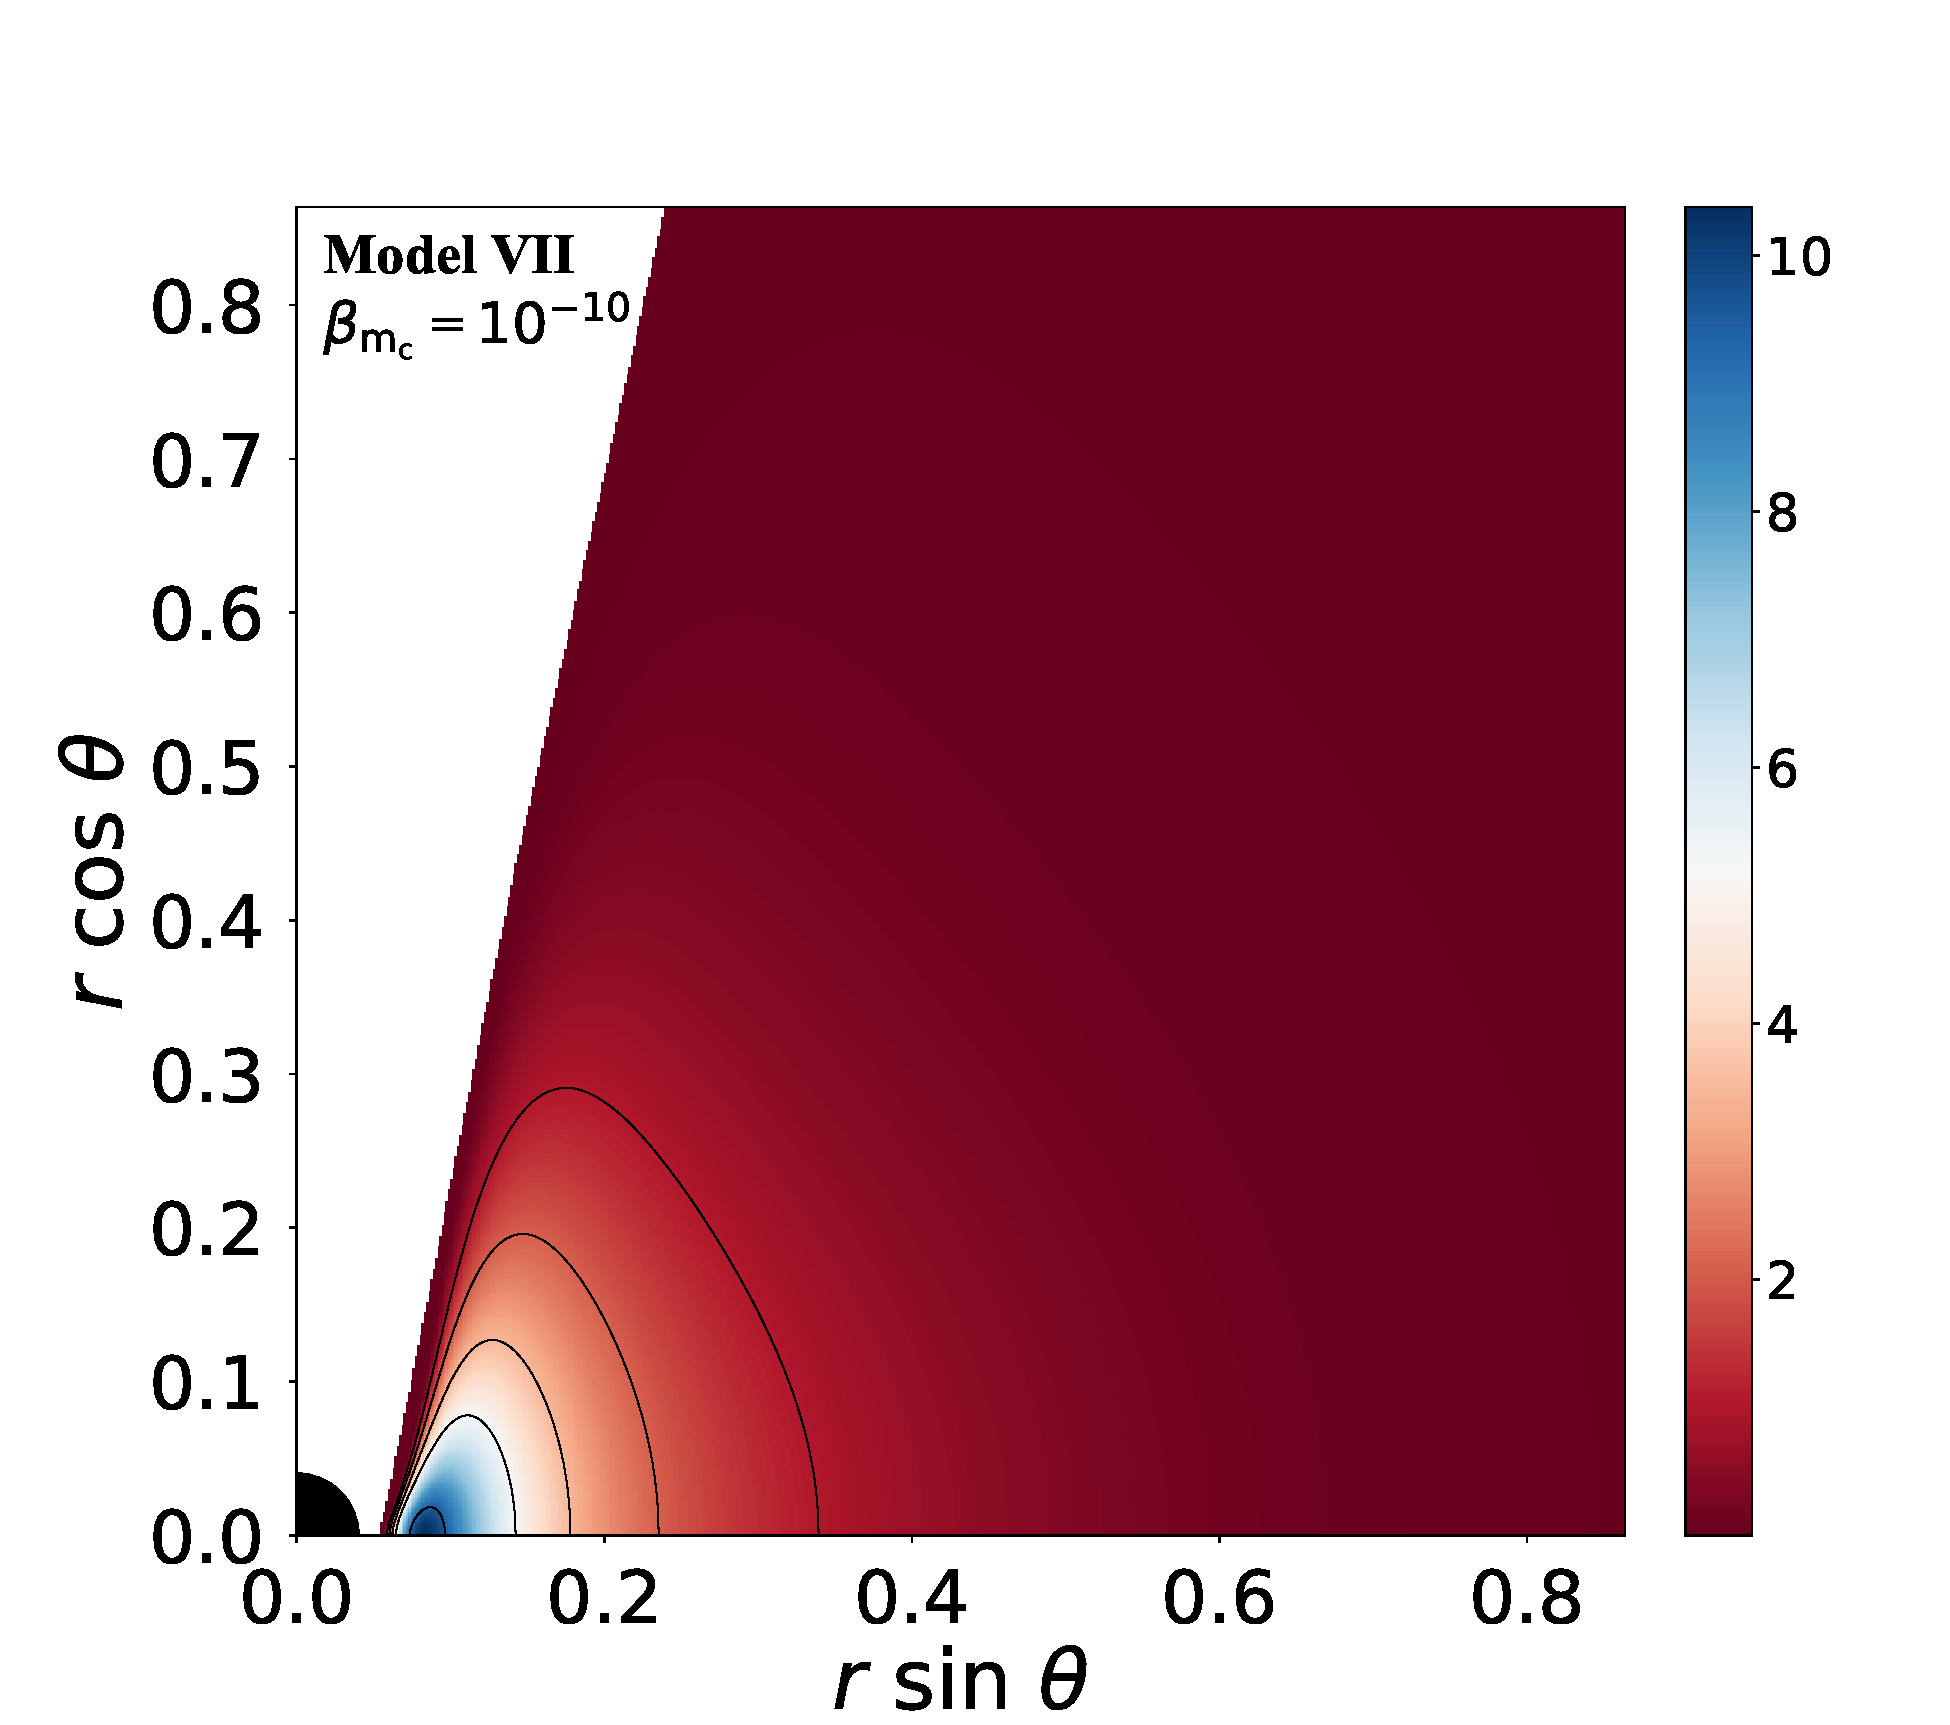
\includegraphics[scale=0.14]{figures/fig2_VII__10.pdf}
\hspace{-0.2cm}
\caption{Rest-mass density distribution. From top to bottom the rows correspond to the different models for the KBHsSH (V, VI and VII). From left to right the columns correspond to different values of the magnetization parameter, namely non-magnetized ($\beta_{\mathrm{m}_{\mathrm{c}}} = 10^{10}$), mildly magnetized ($\beta_{\mathrm{m}_{\mathrm{c}}} = 1$) and strongly magnetized ($\beta_{\mathrm{m}_{\mathrm{c}}} = 10^{-10}$)}
\label{models_II}
\end{figure*}

\begin{figure*}
\centering
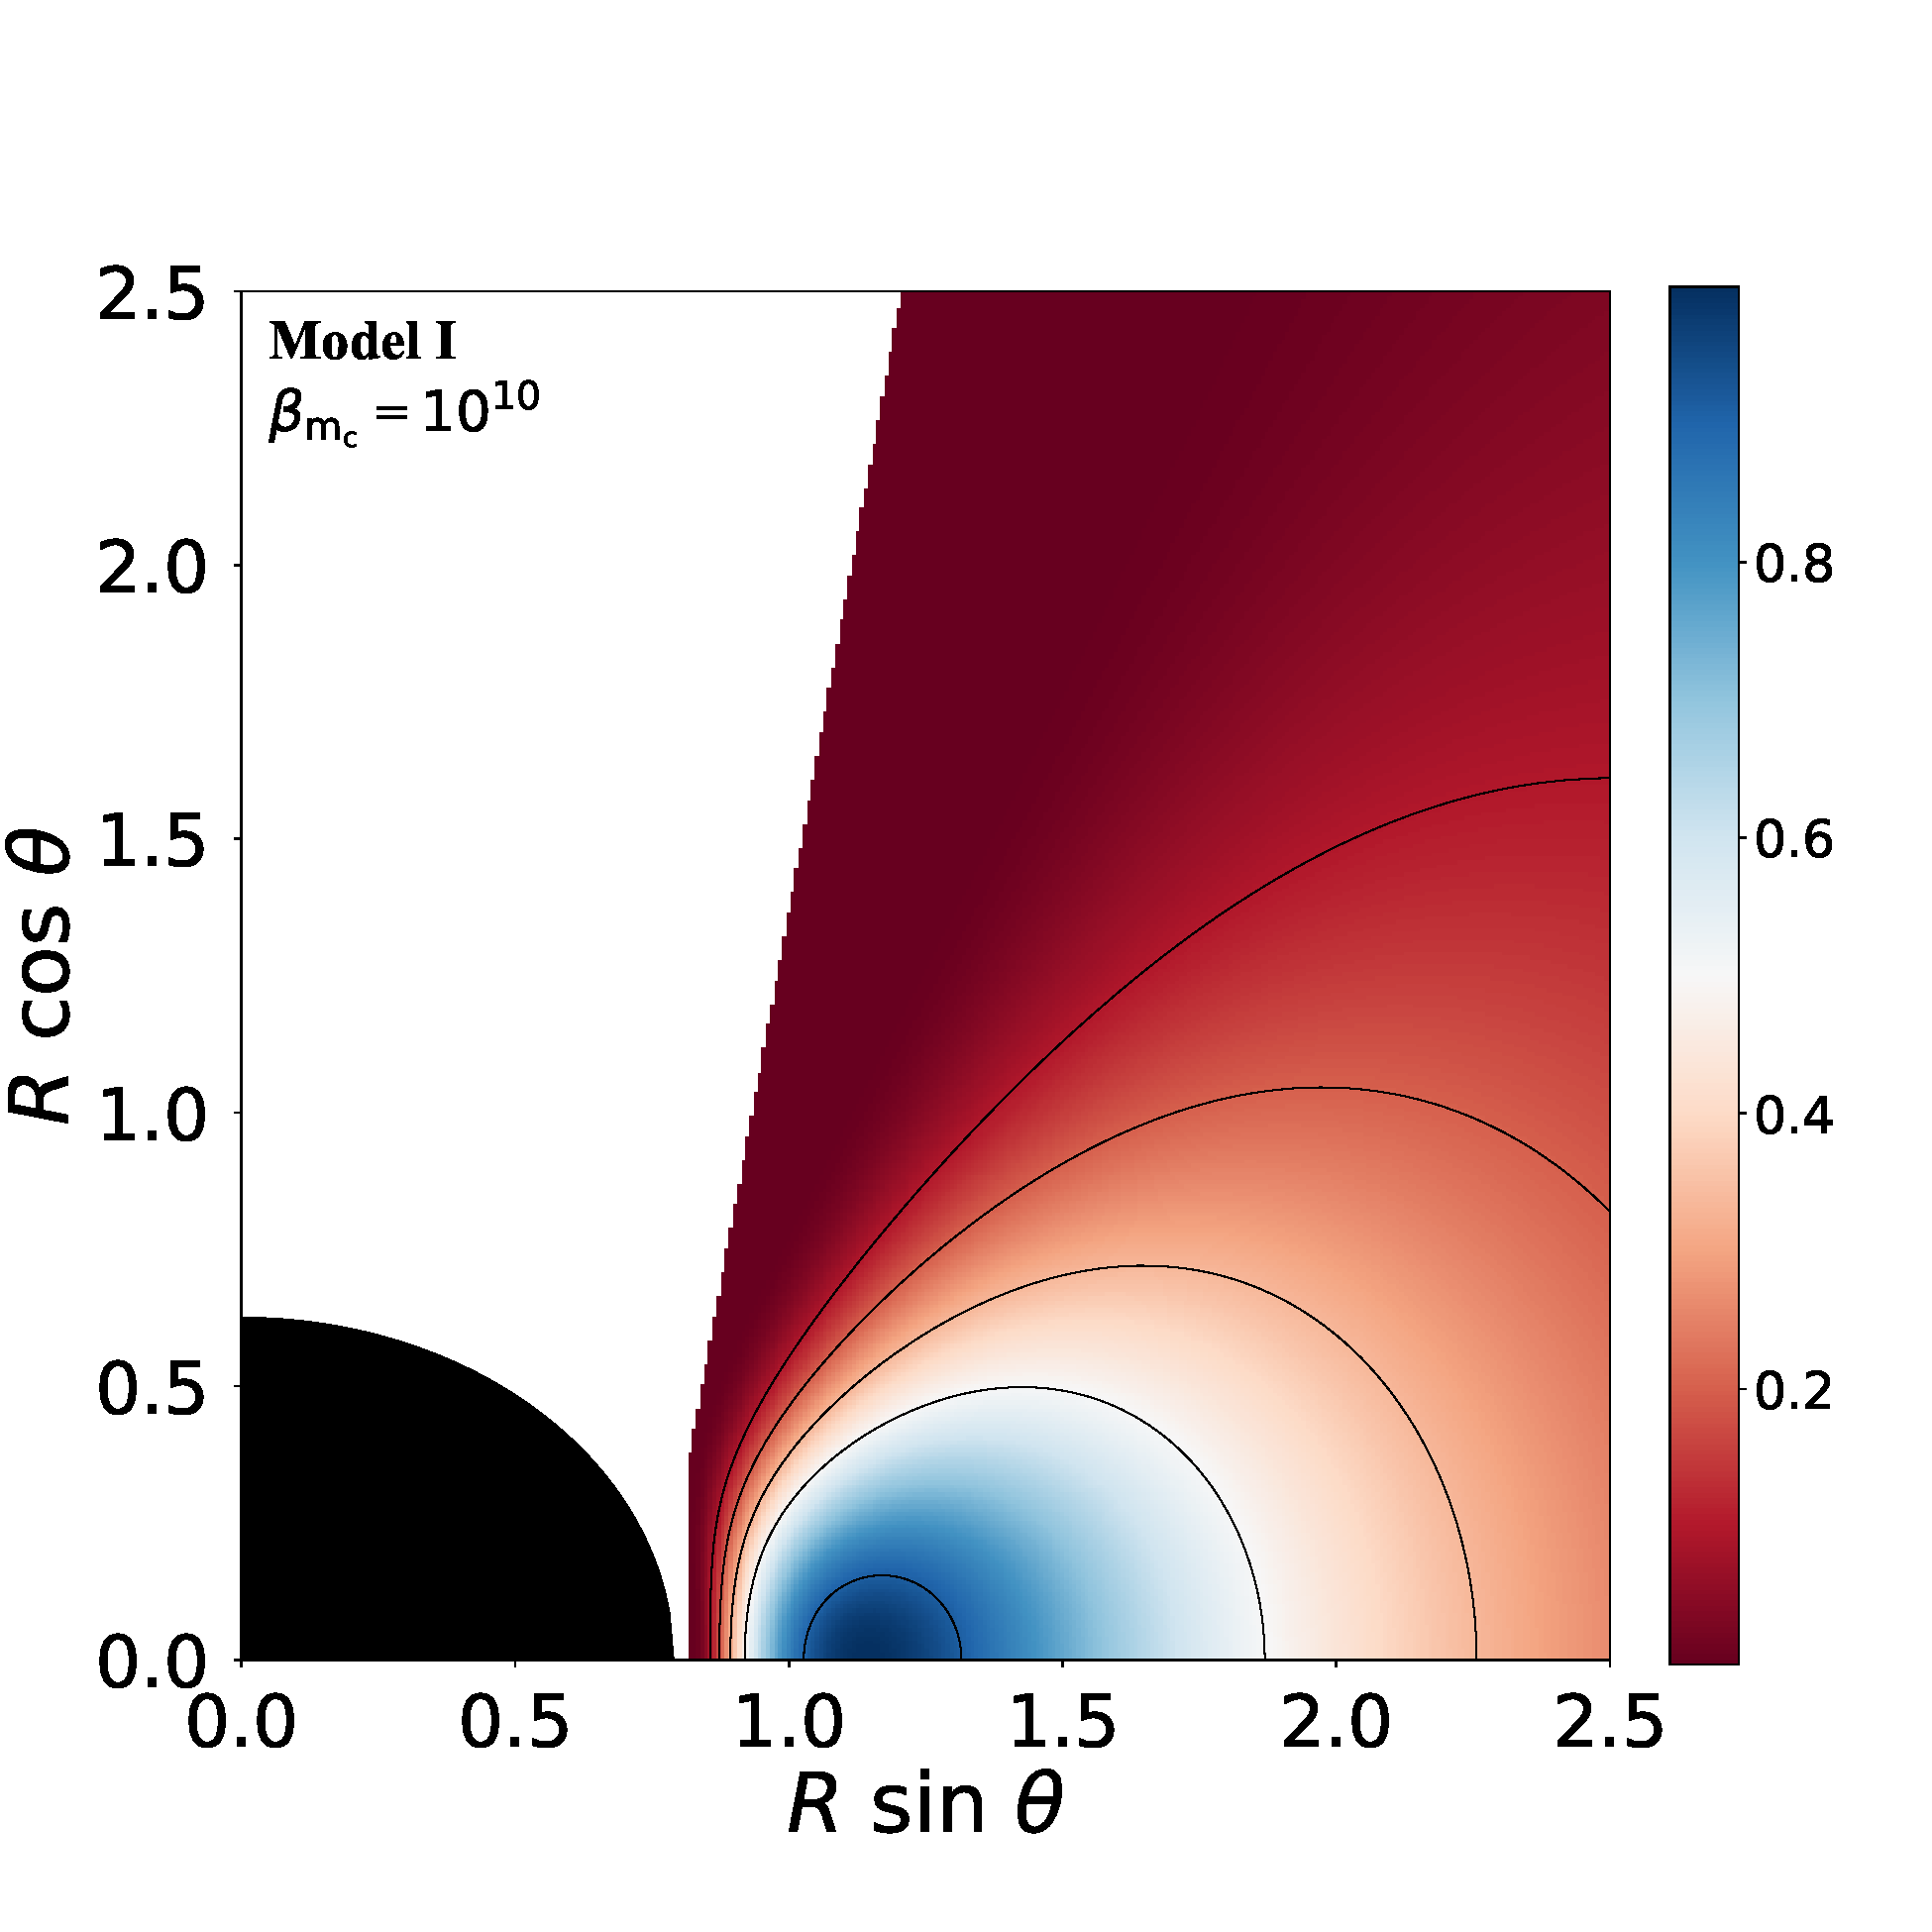
\includegraphics[scale=0.14]{figures/fig3_I_10.pdf}
\hspace{-0.3cm}
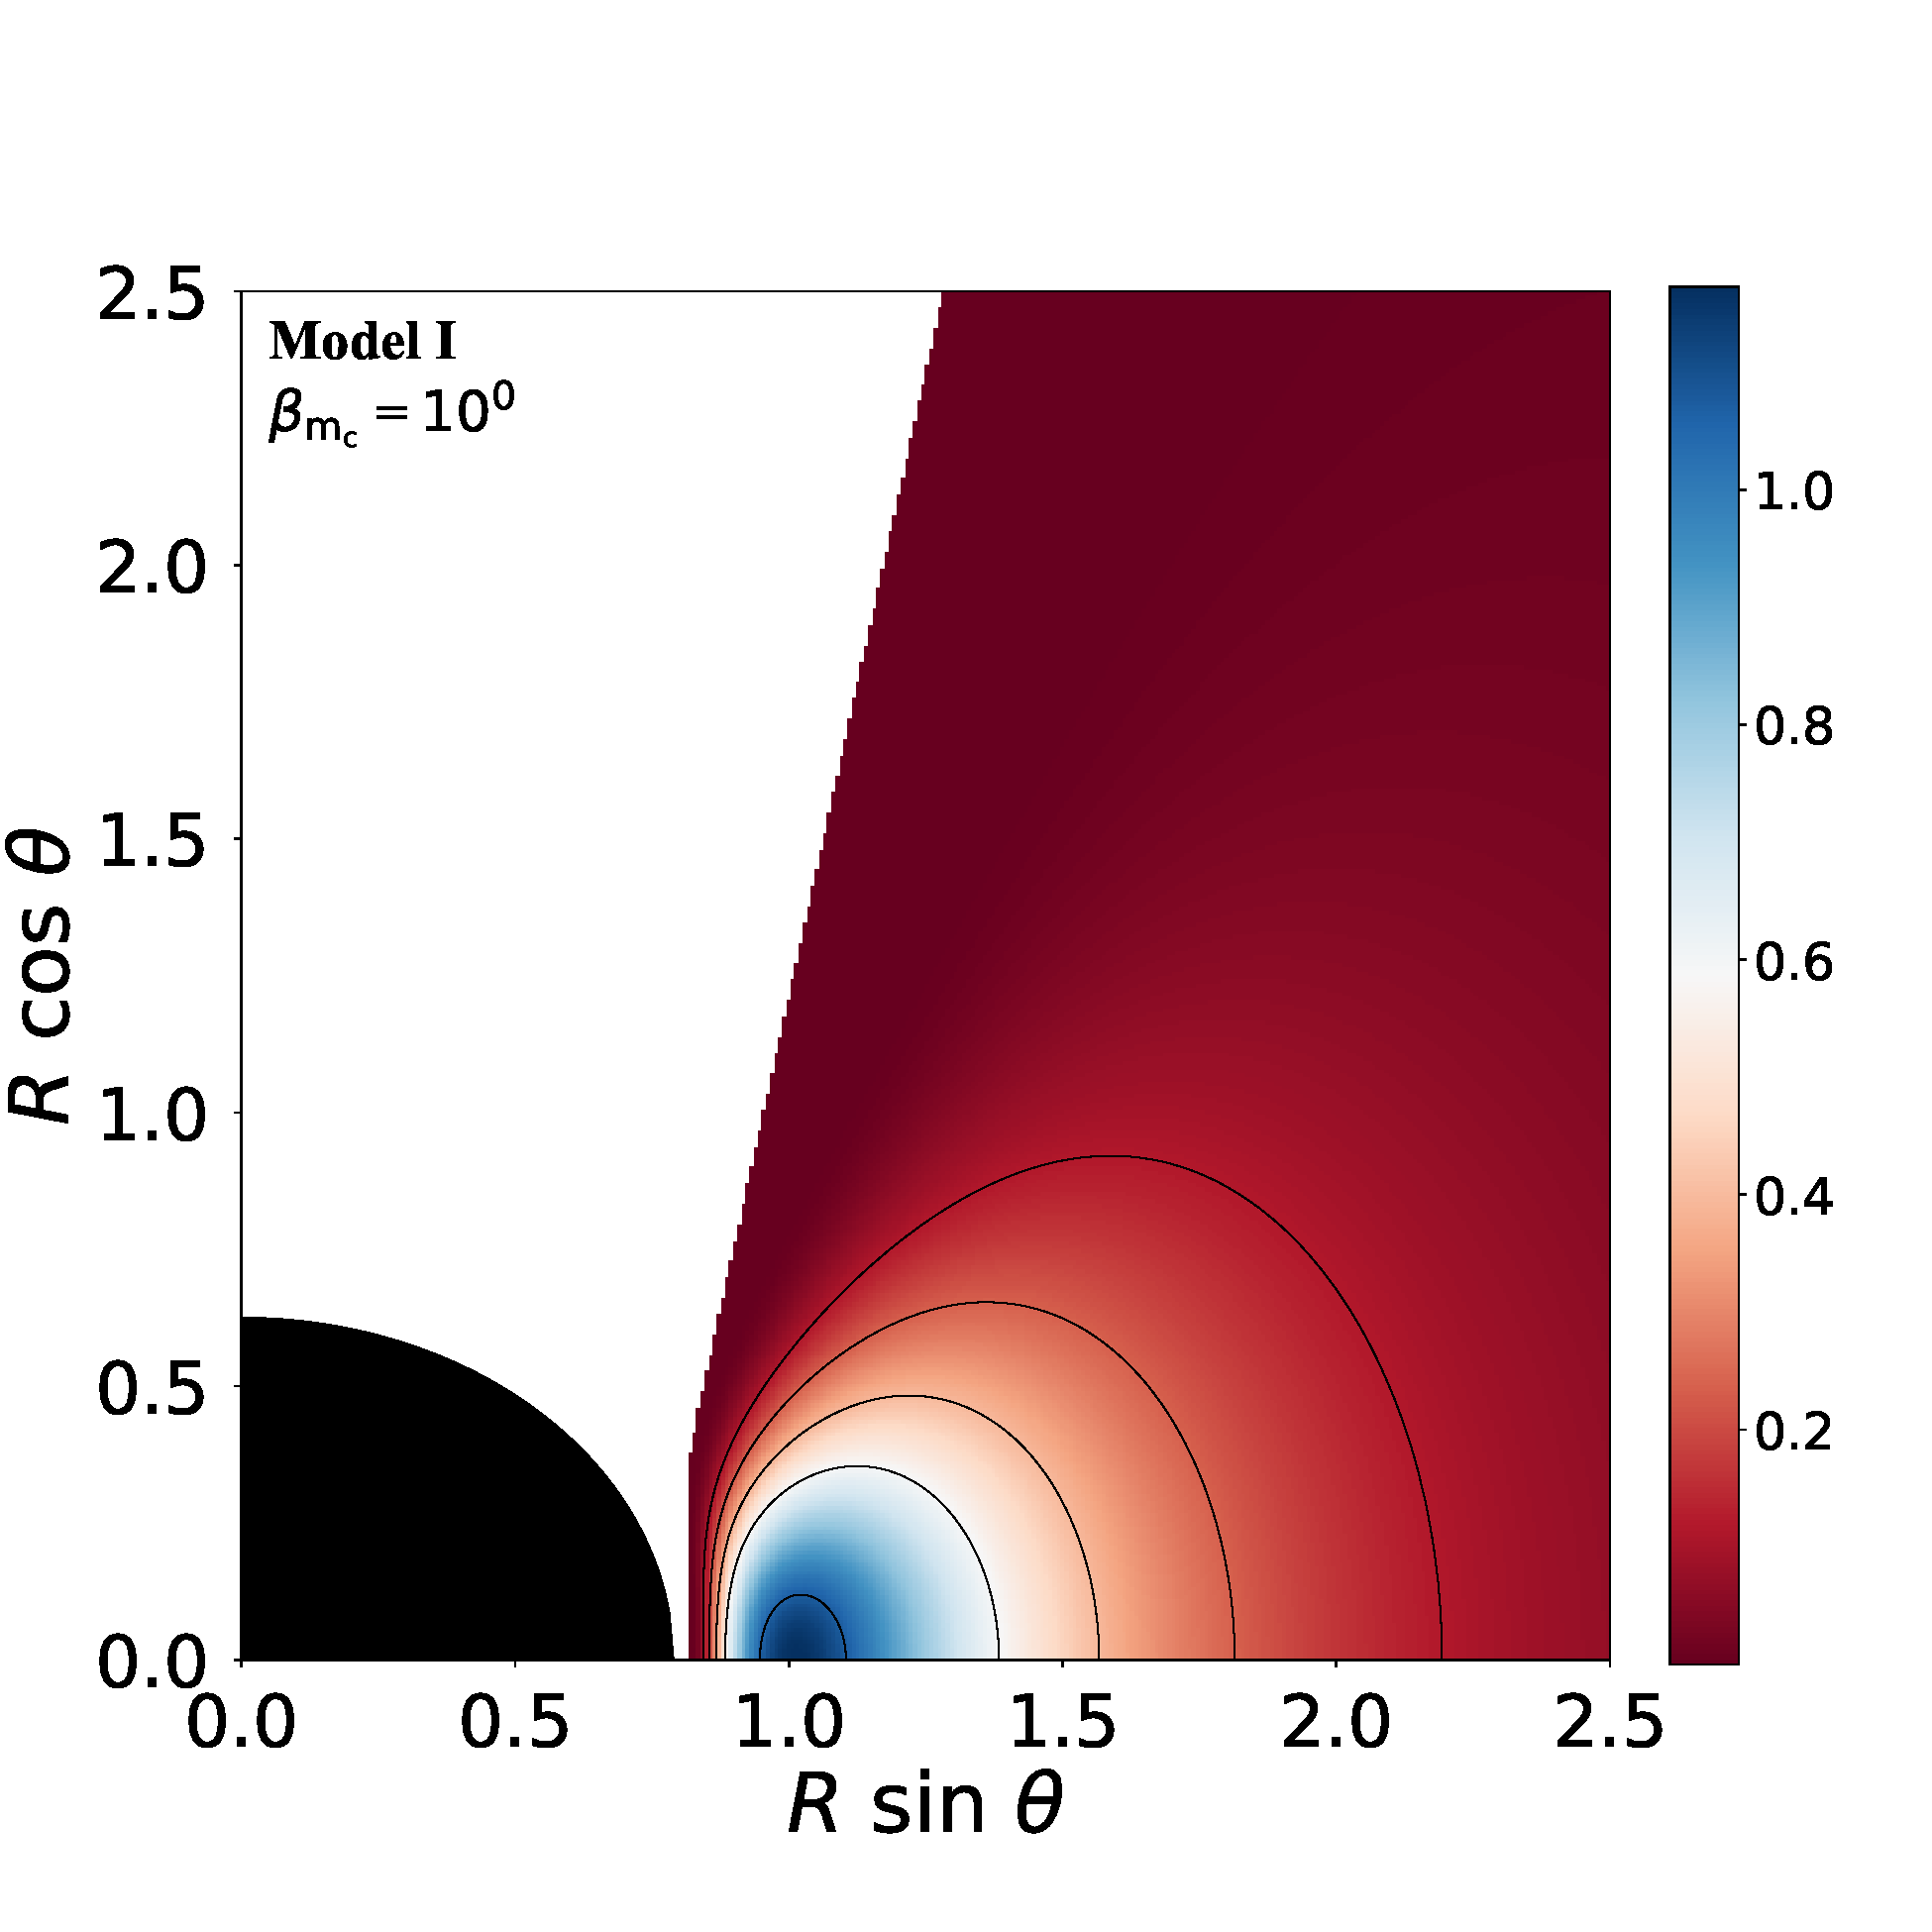
\includegraphics[scale=0.14]{figures/fig3_I_1.pdf}
\hspace{-0.2cm}
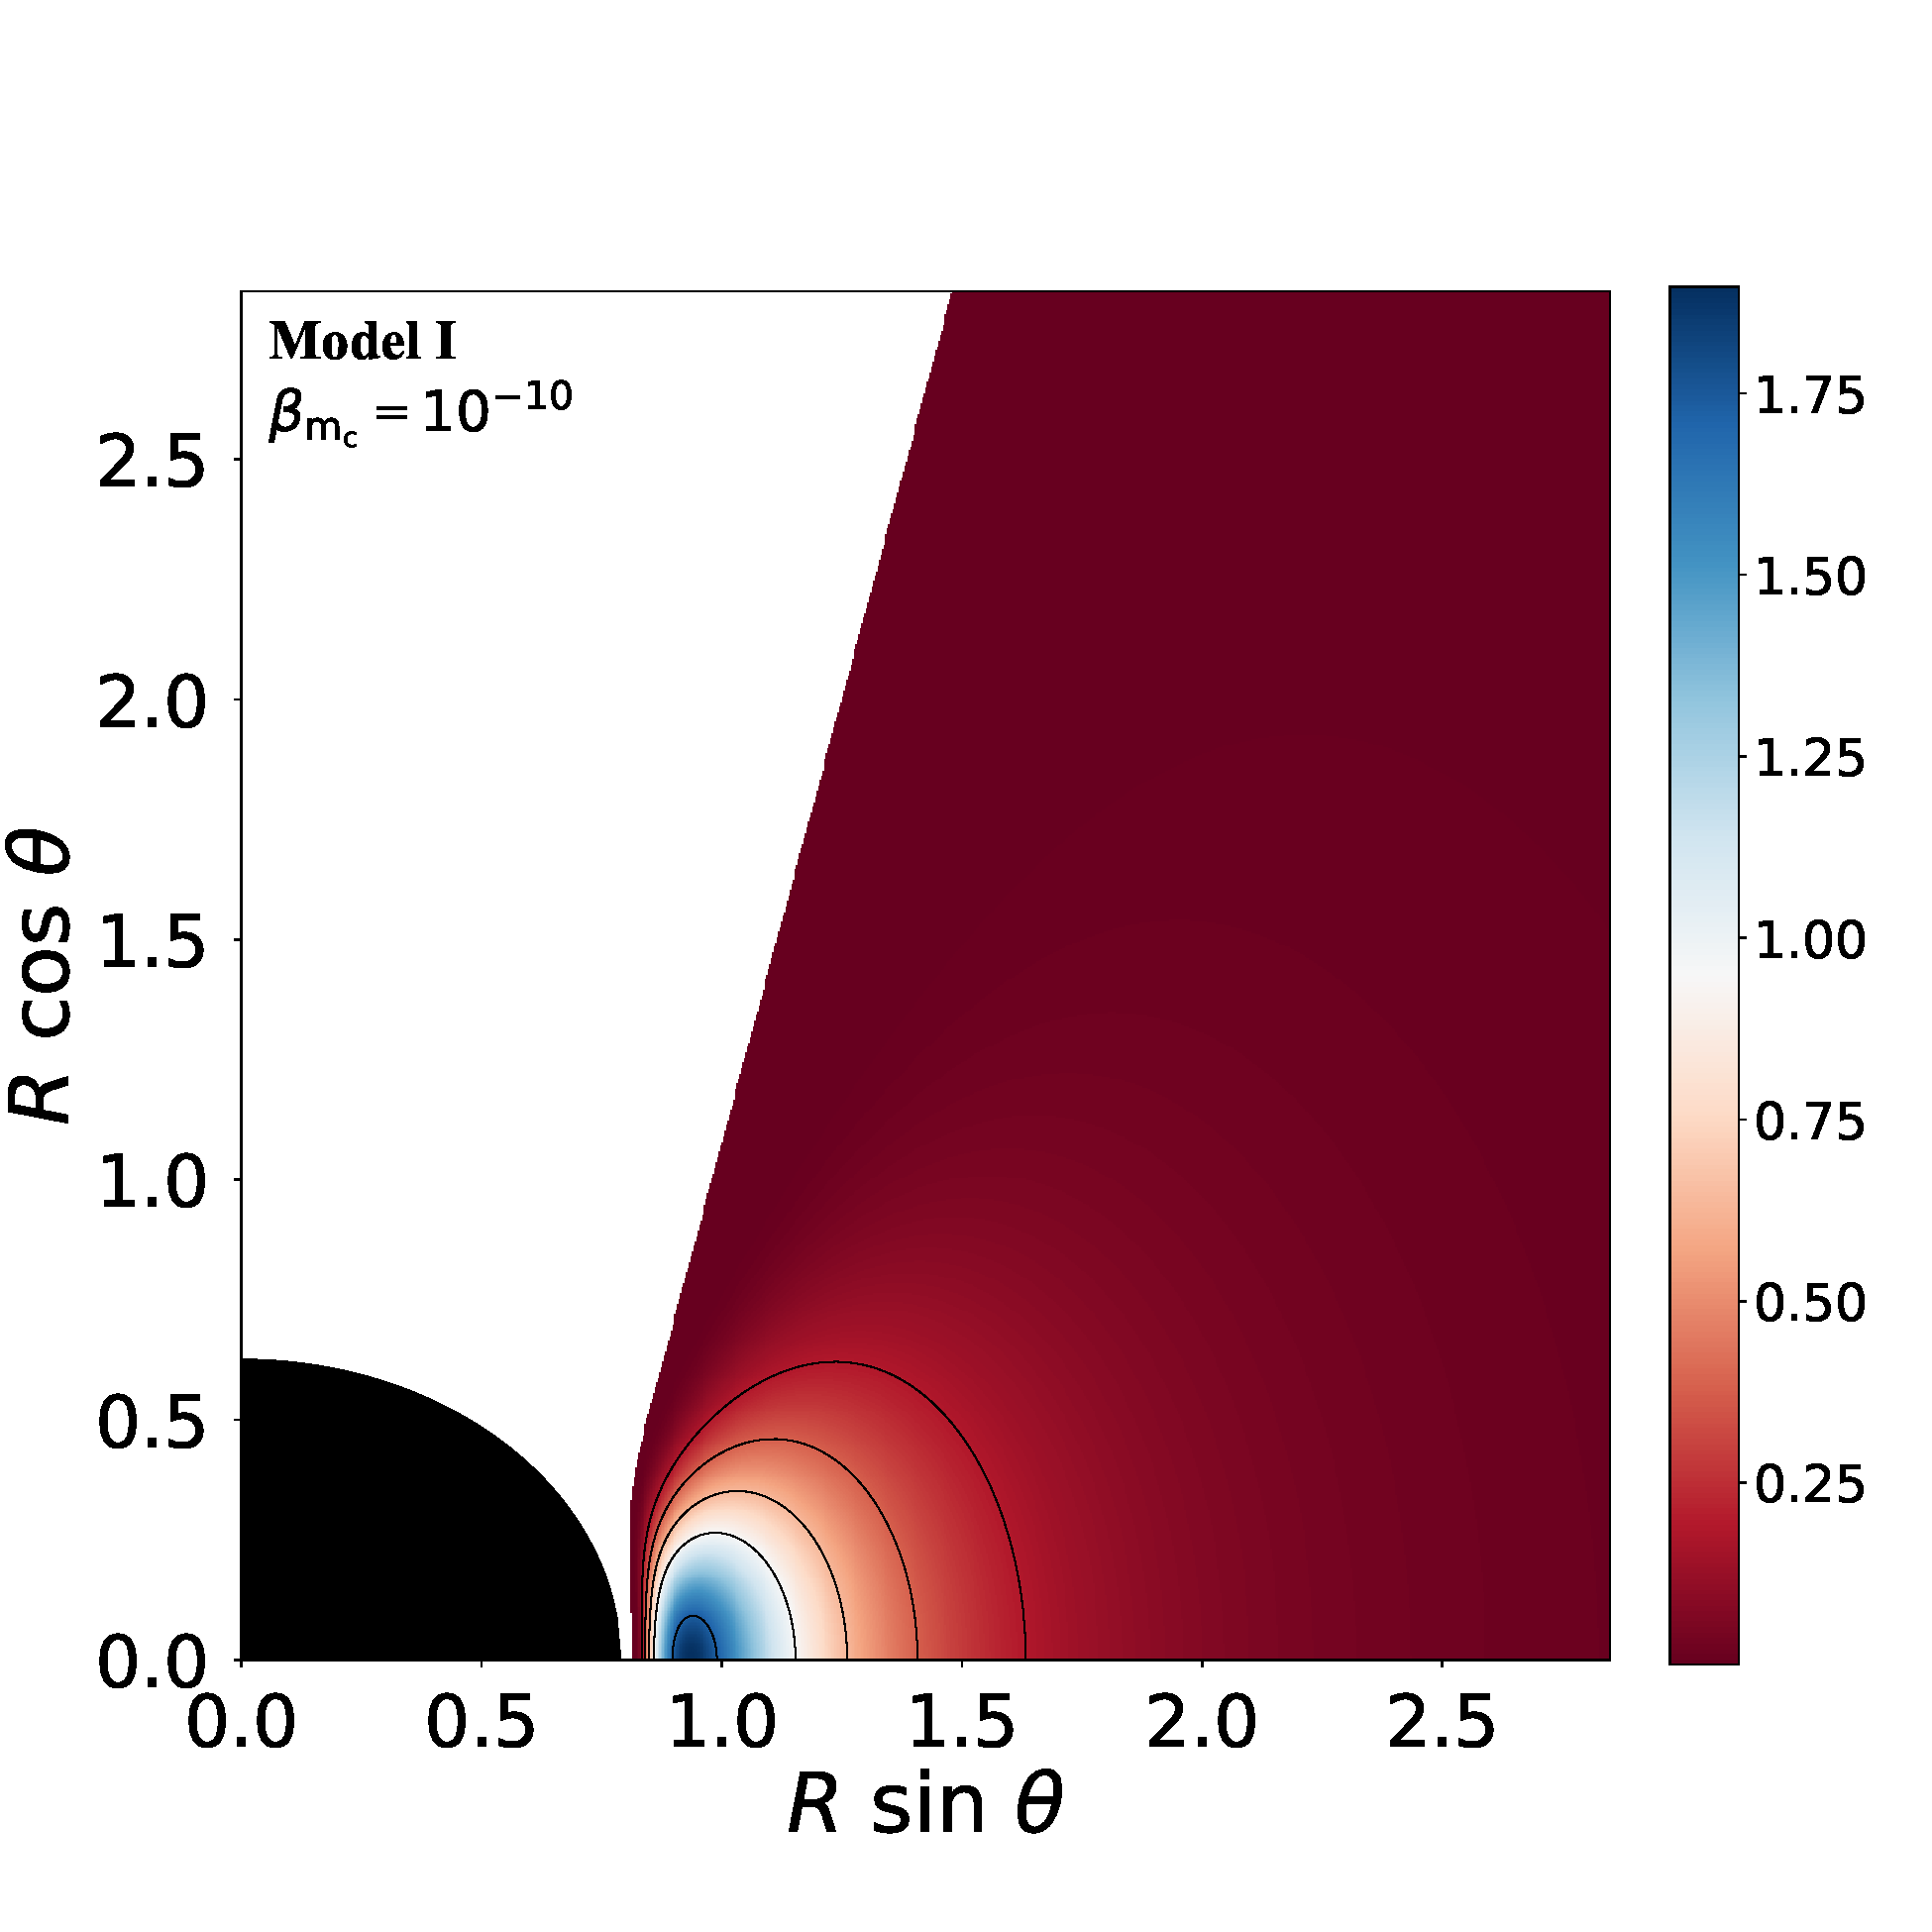
\includegraphics[scale=0.14]{figures/fig3_I__10.pdf}
\\
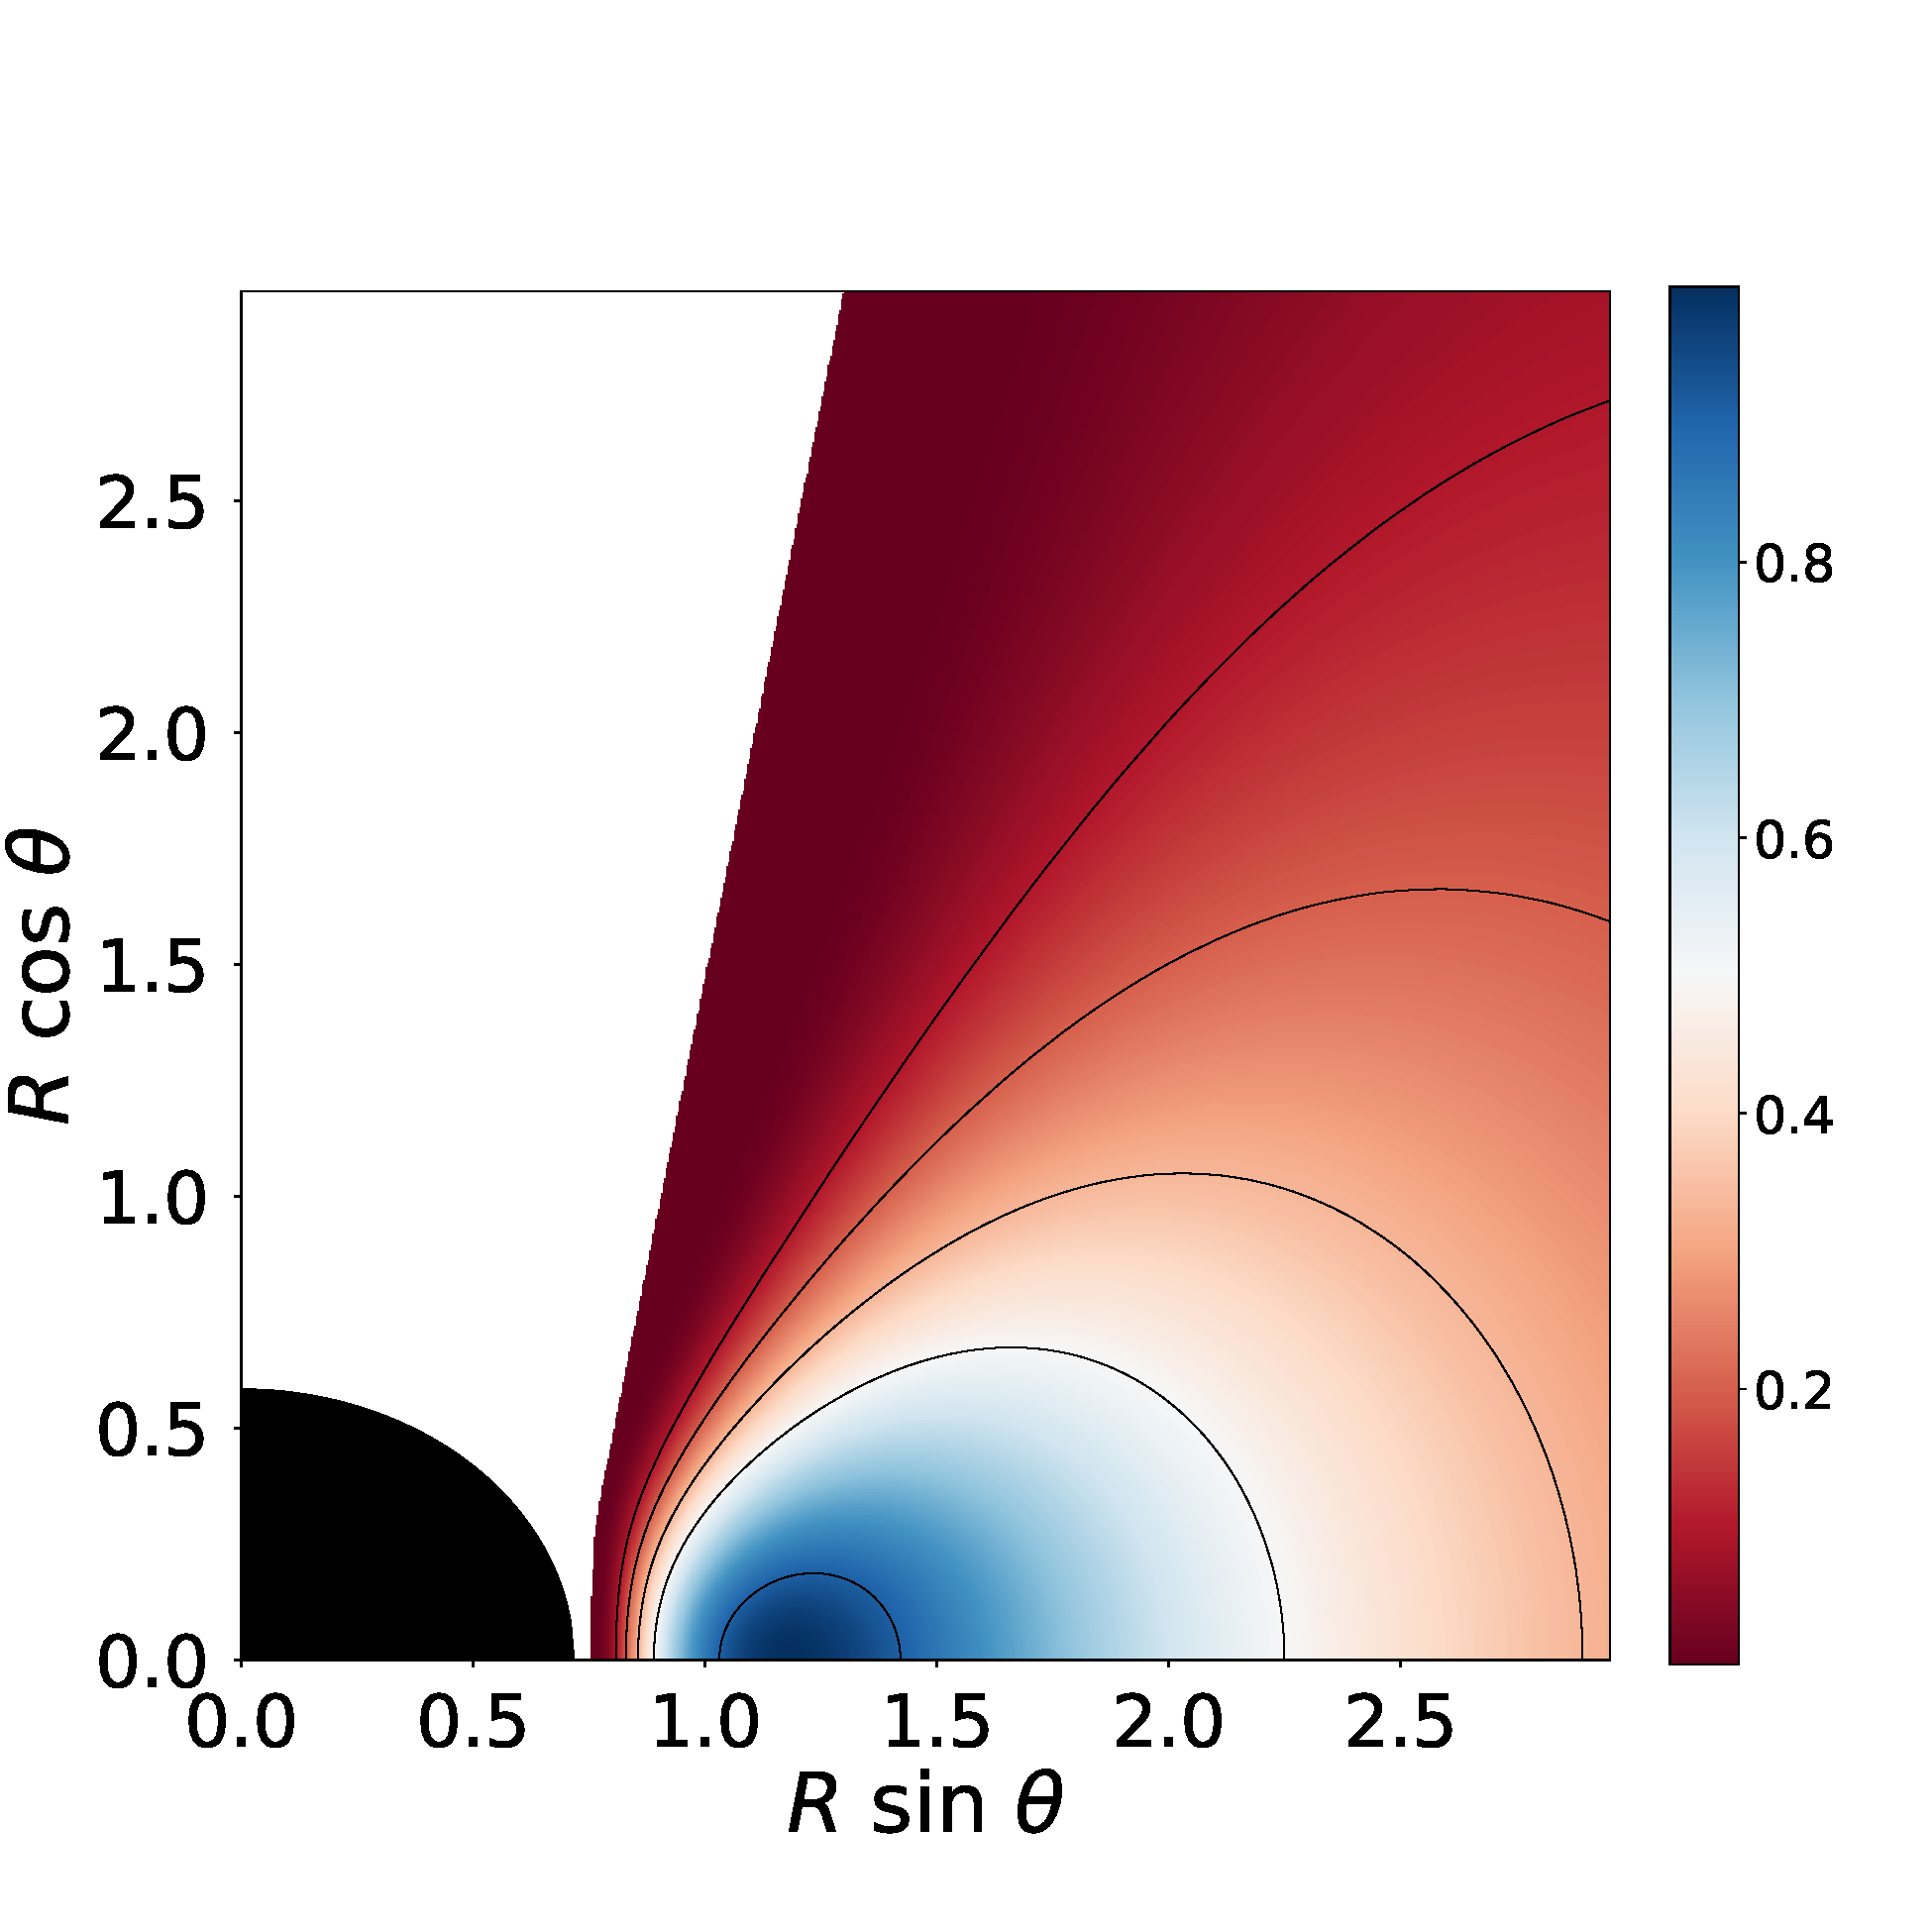
\includegraphics[scale=0.14]{figures/fig3_II_10.pdf}
\hspace{-0.3cm}
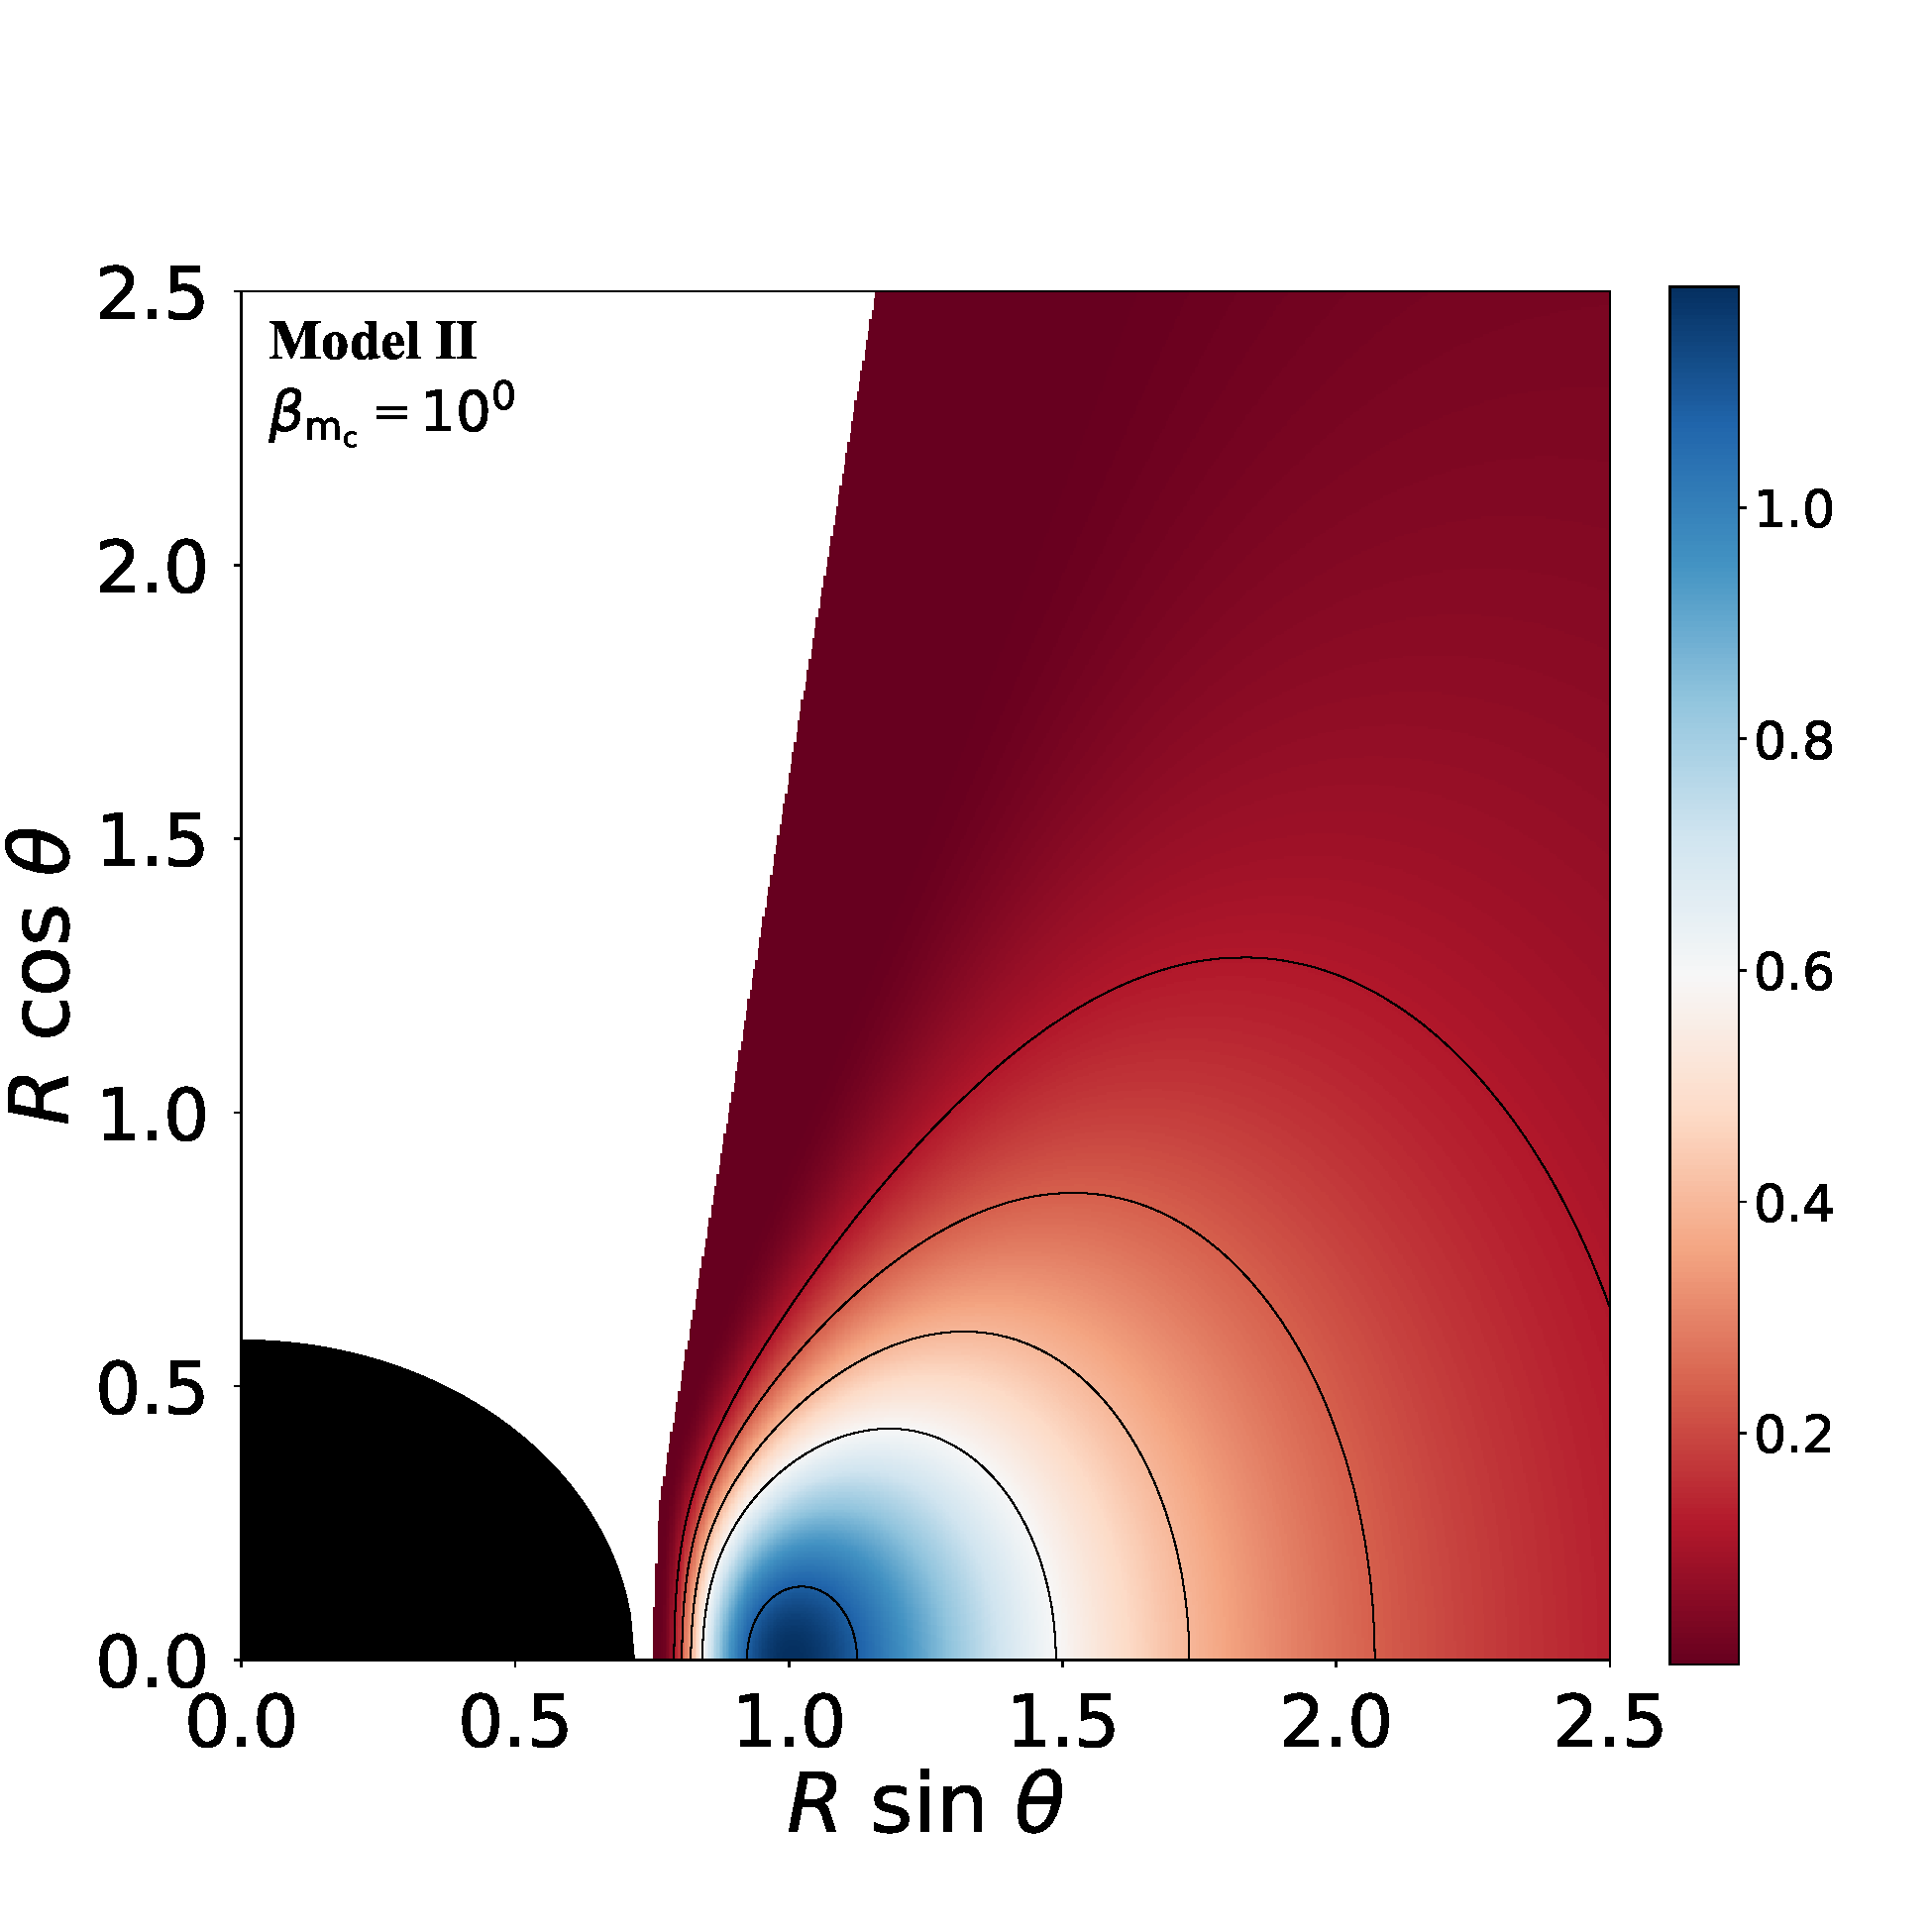
\includegraphics[scale=0.14]{figures/fig3_II_1.pdf}
\hspace{-0.2cm}
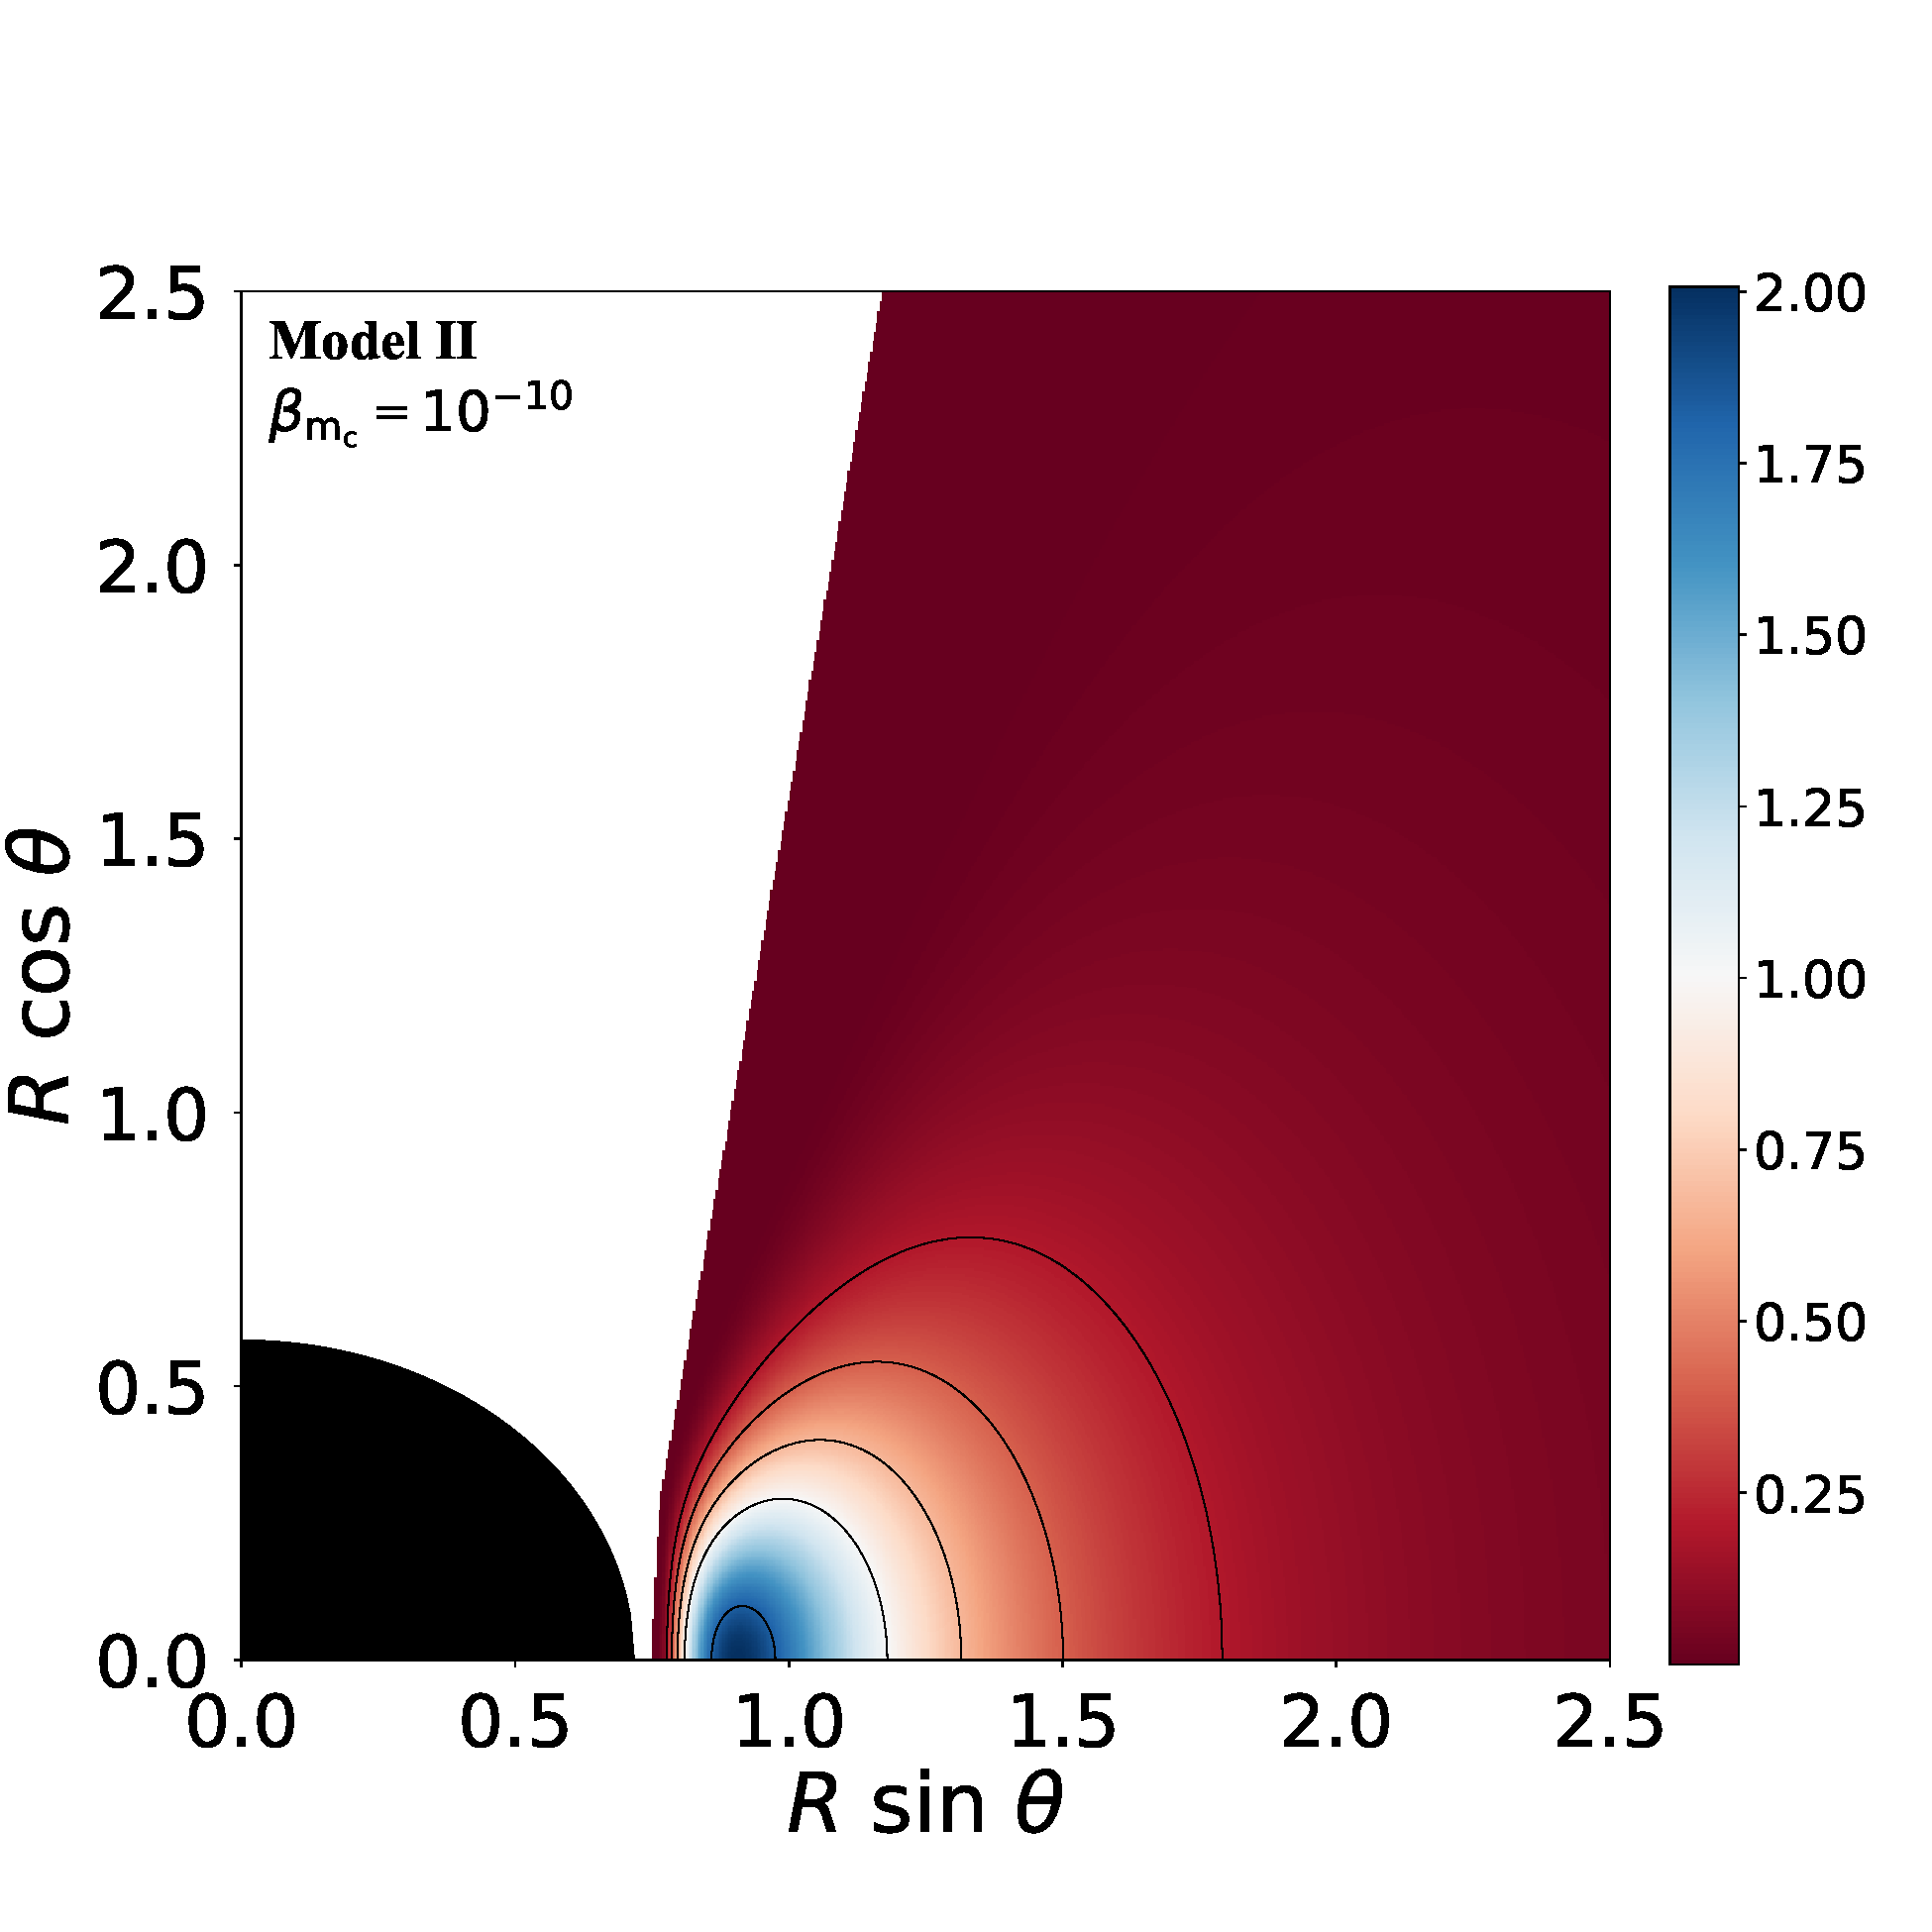
\includegraphics[scale=0.14]{figures/fig3_II__10.pdf}
\\
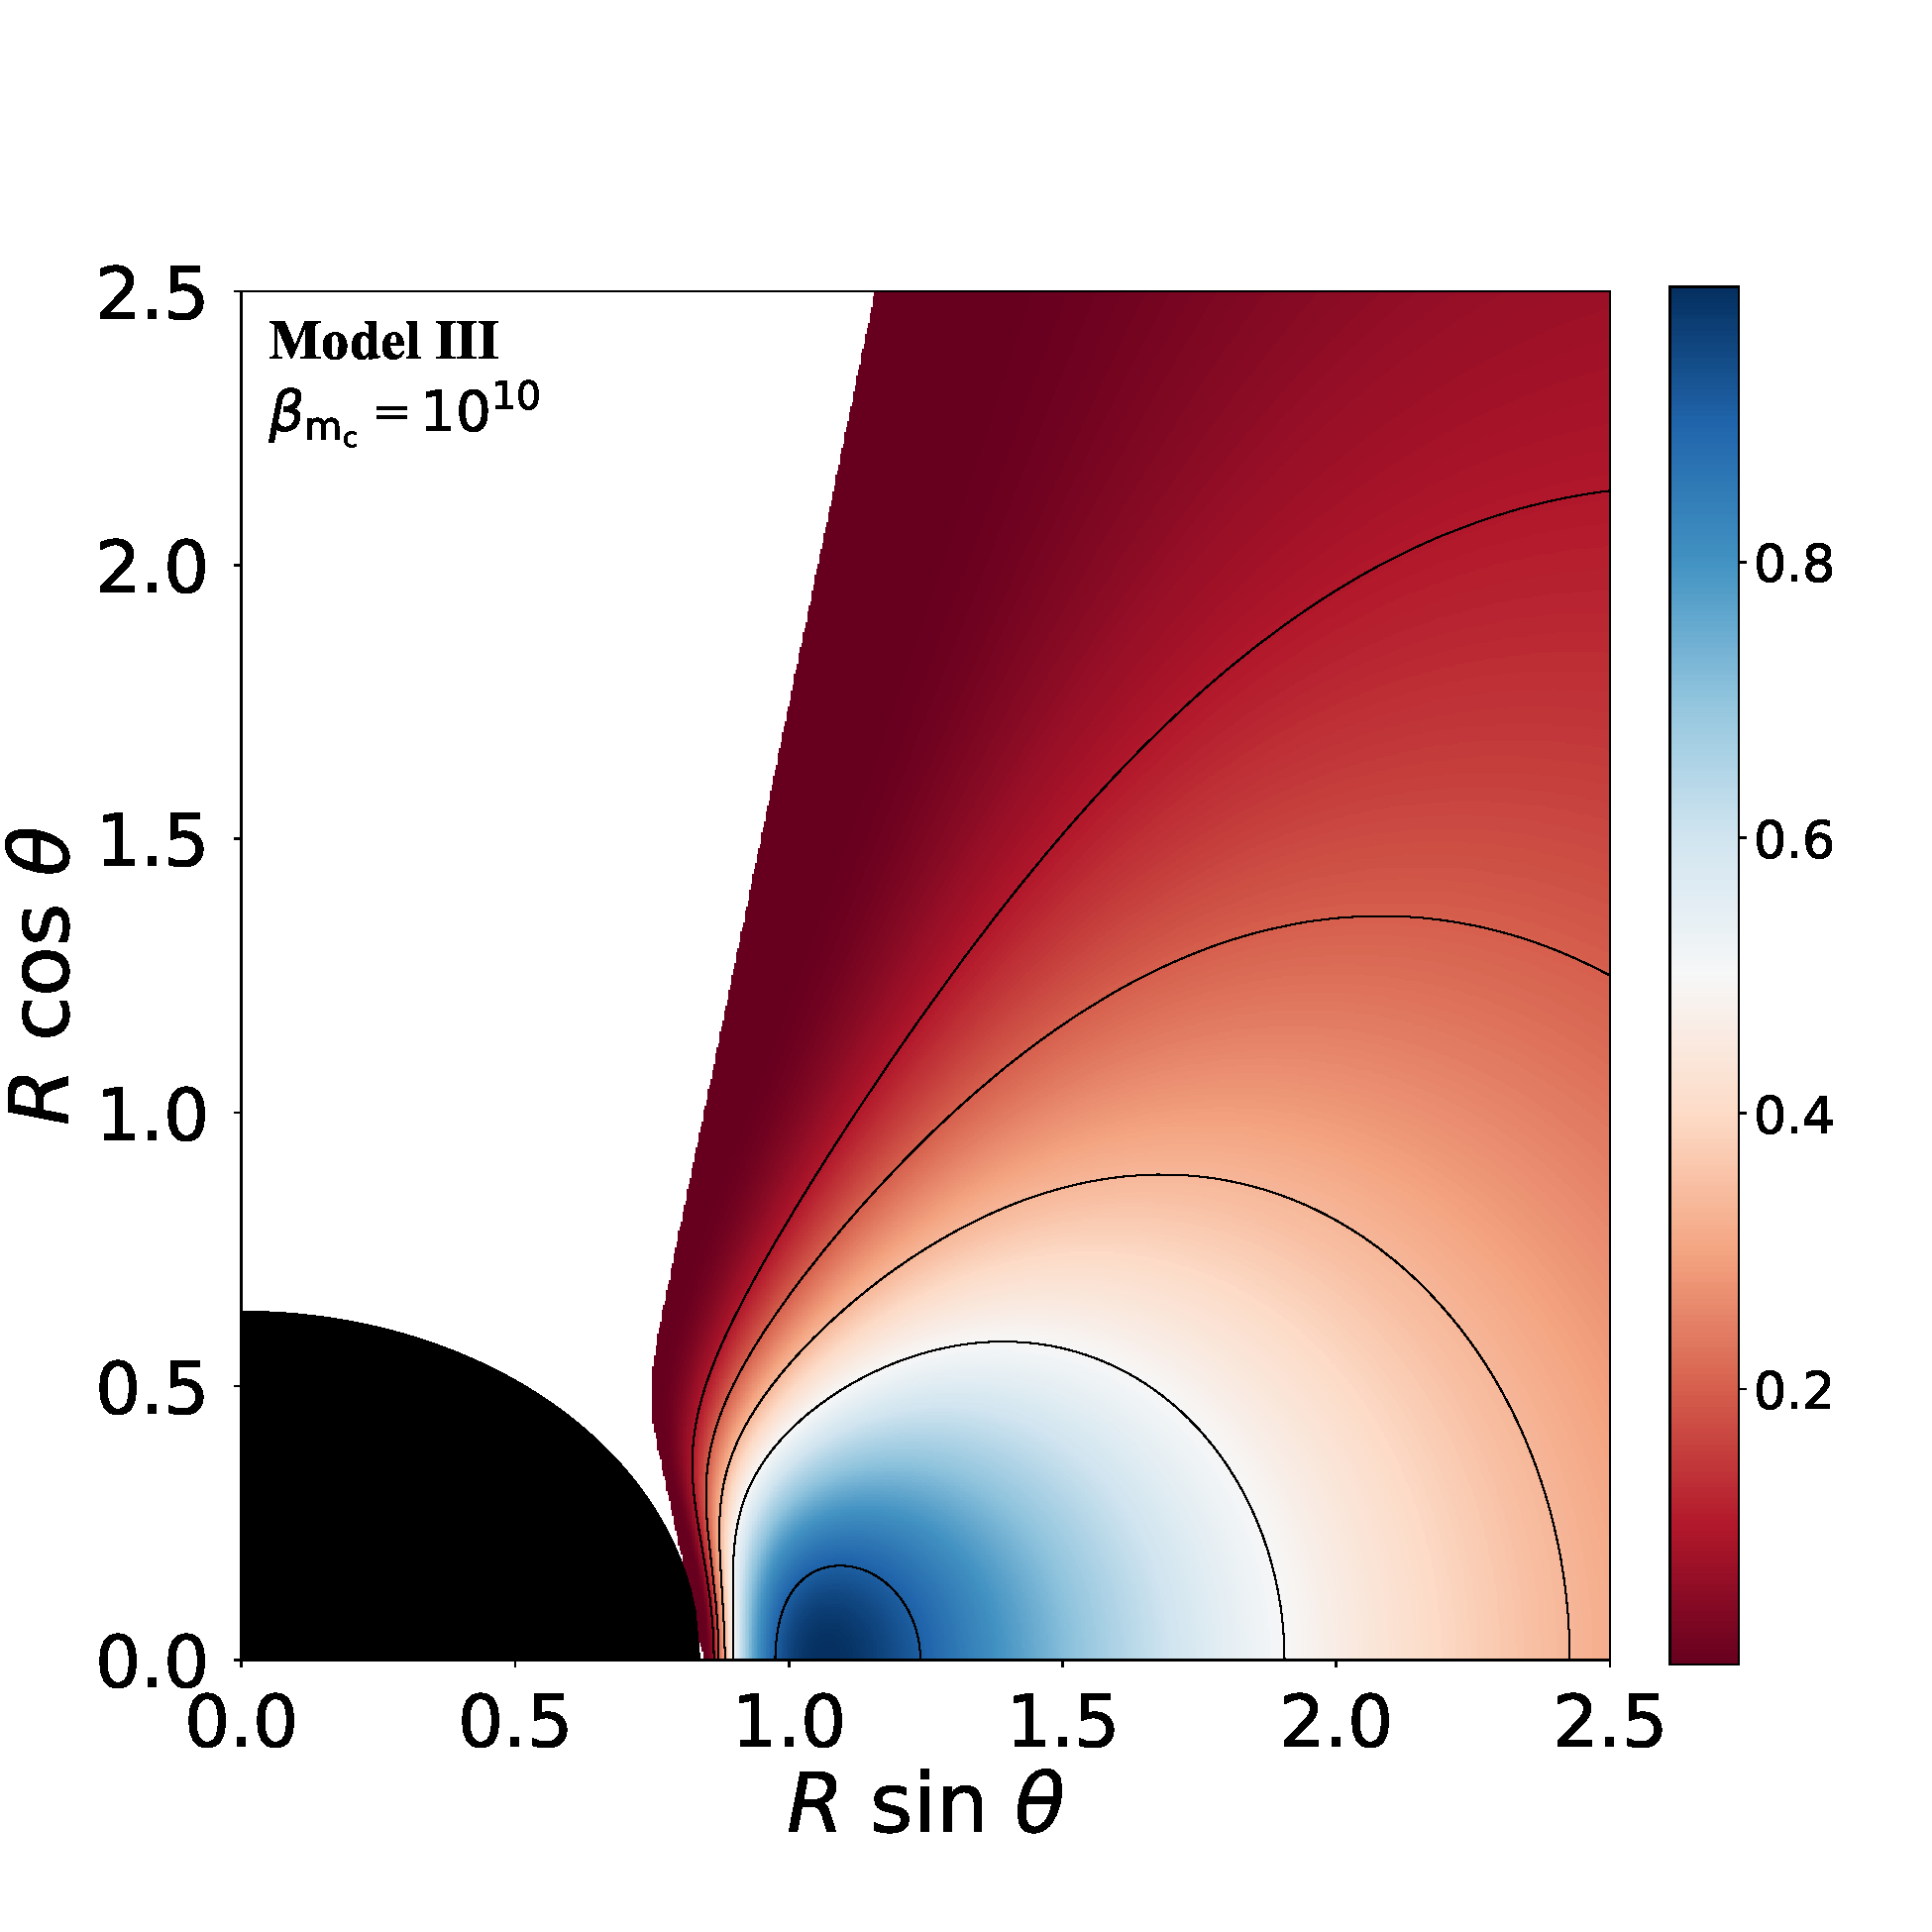
\includegraphics[scale=0.14]{figures/fig3_III_10.pdf}
\hspace{-0.3cm}
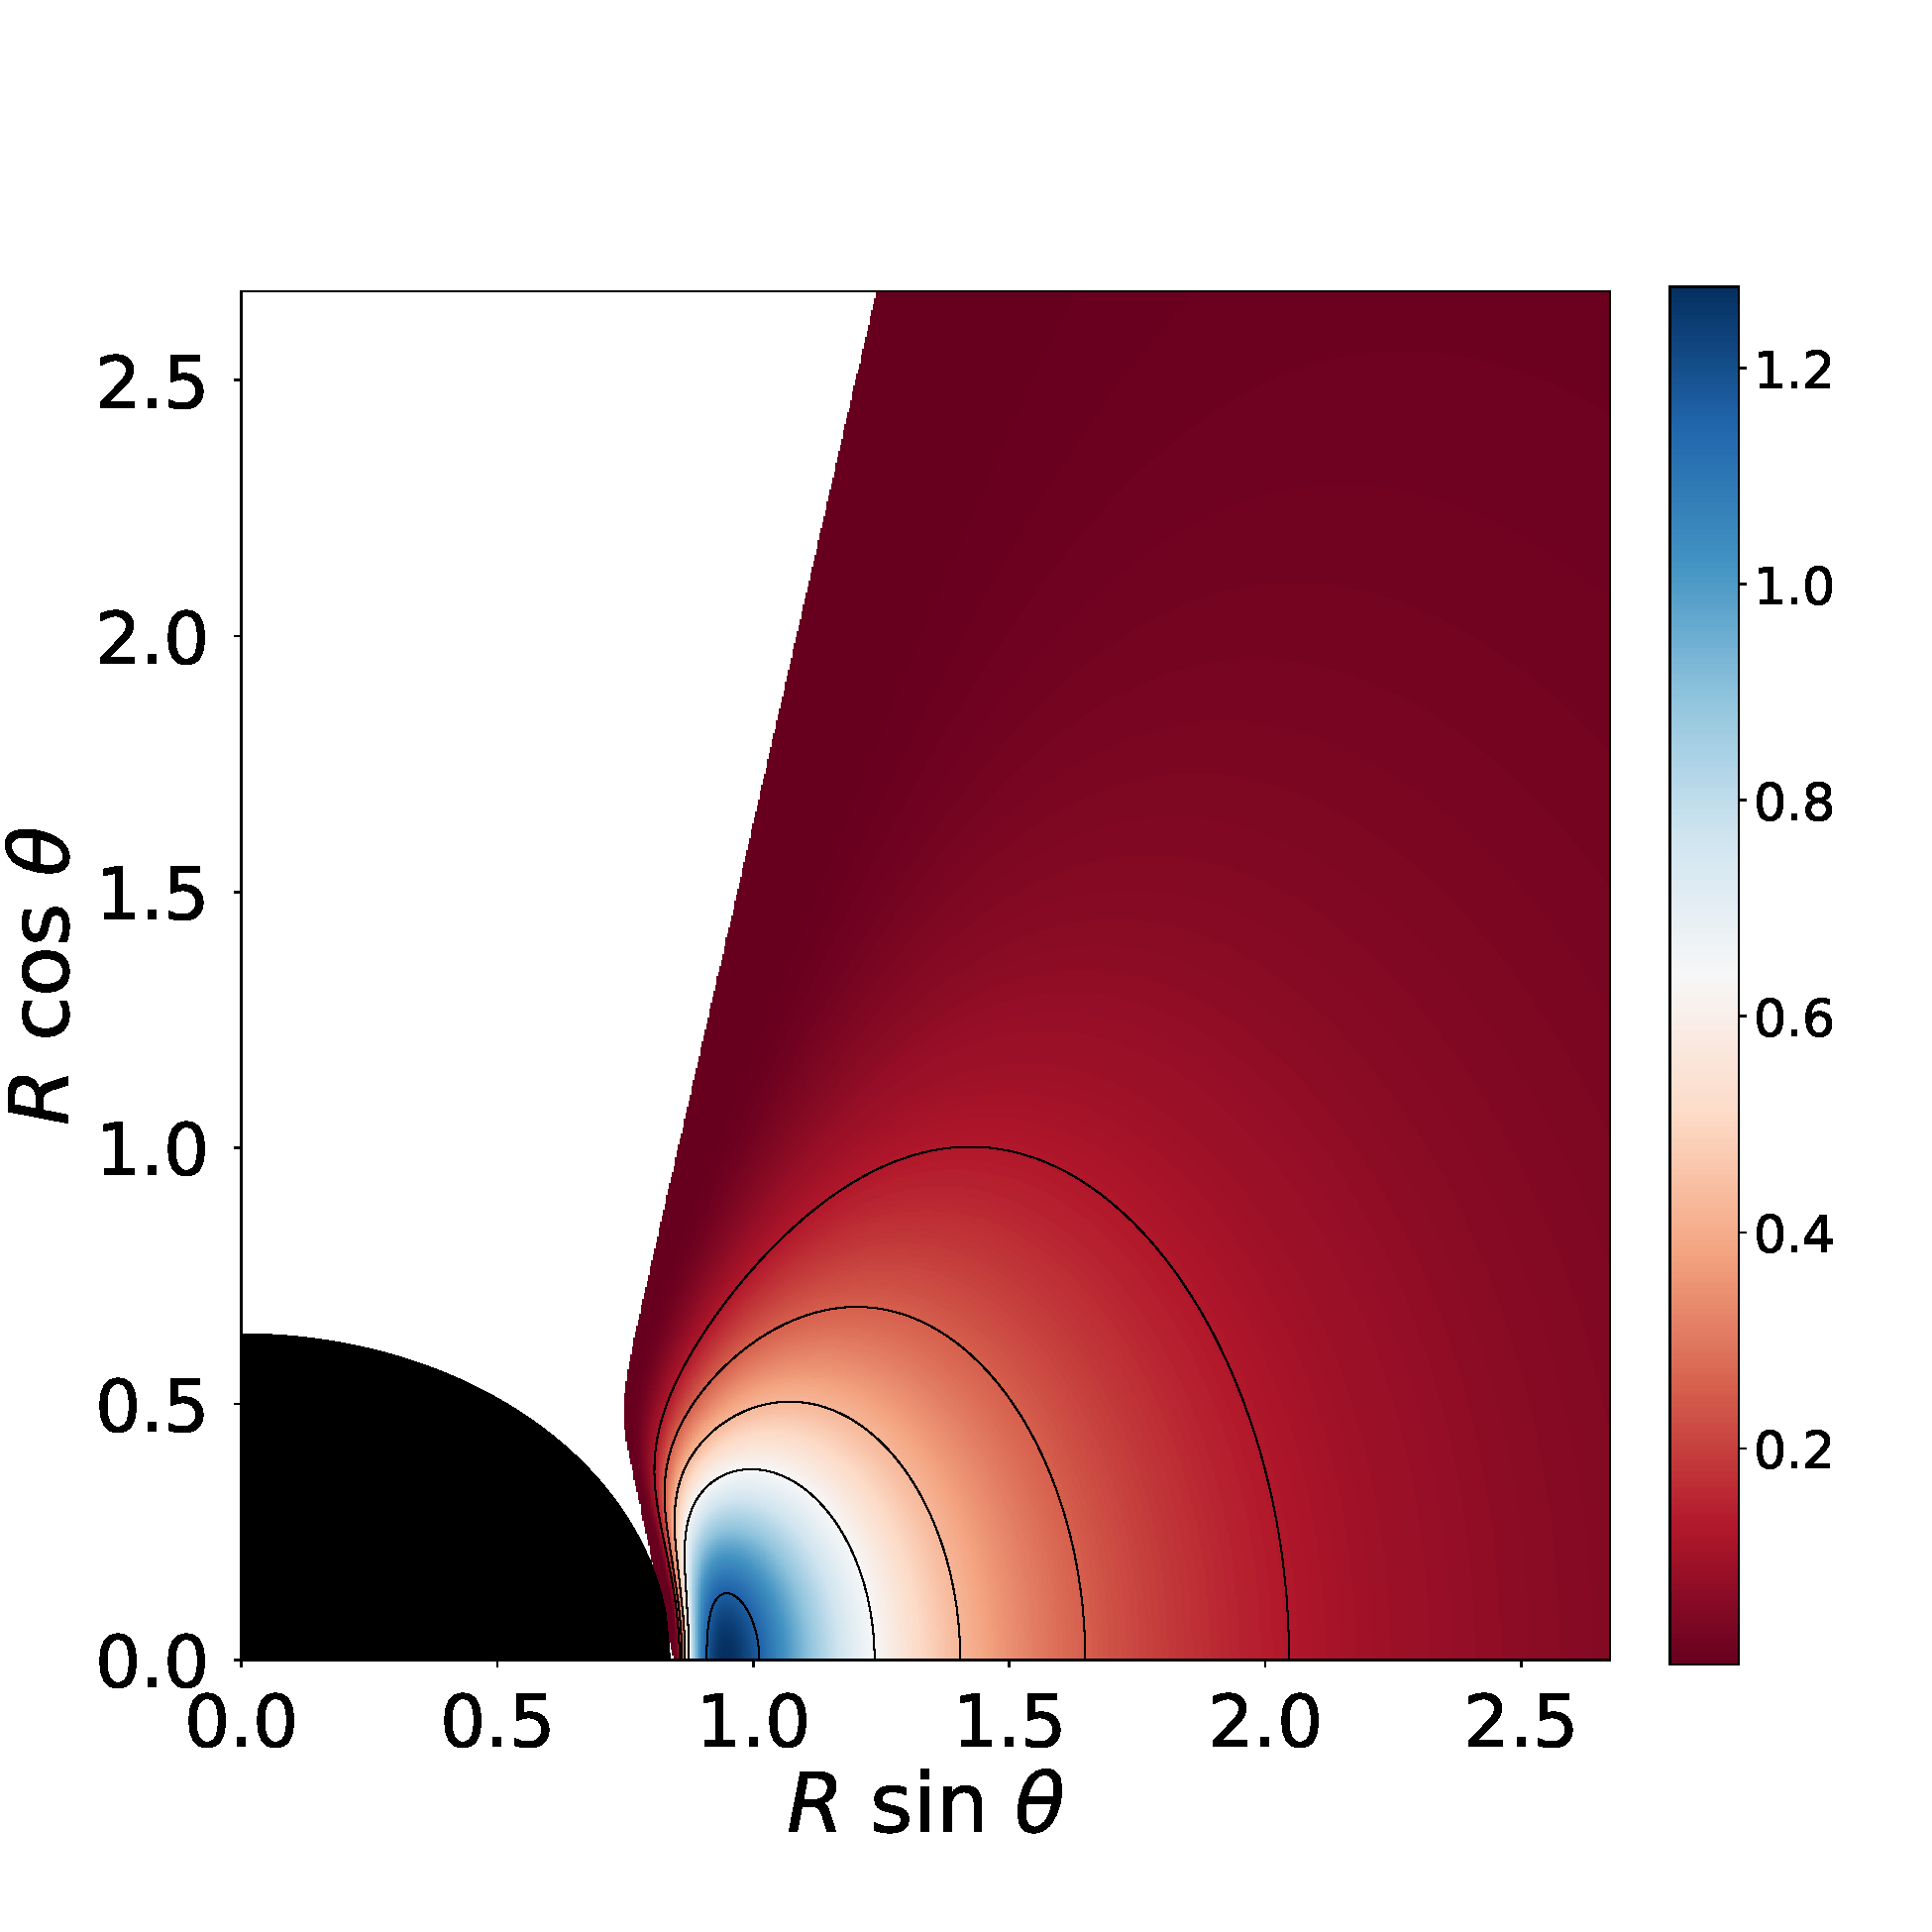
\includegraphics[scale=0.14]{figures/fig3_III_1.pdf}
\hspace{-0.2cm}
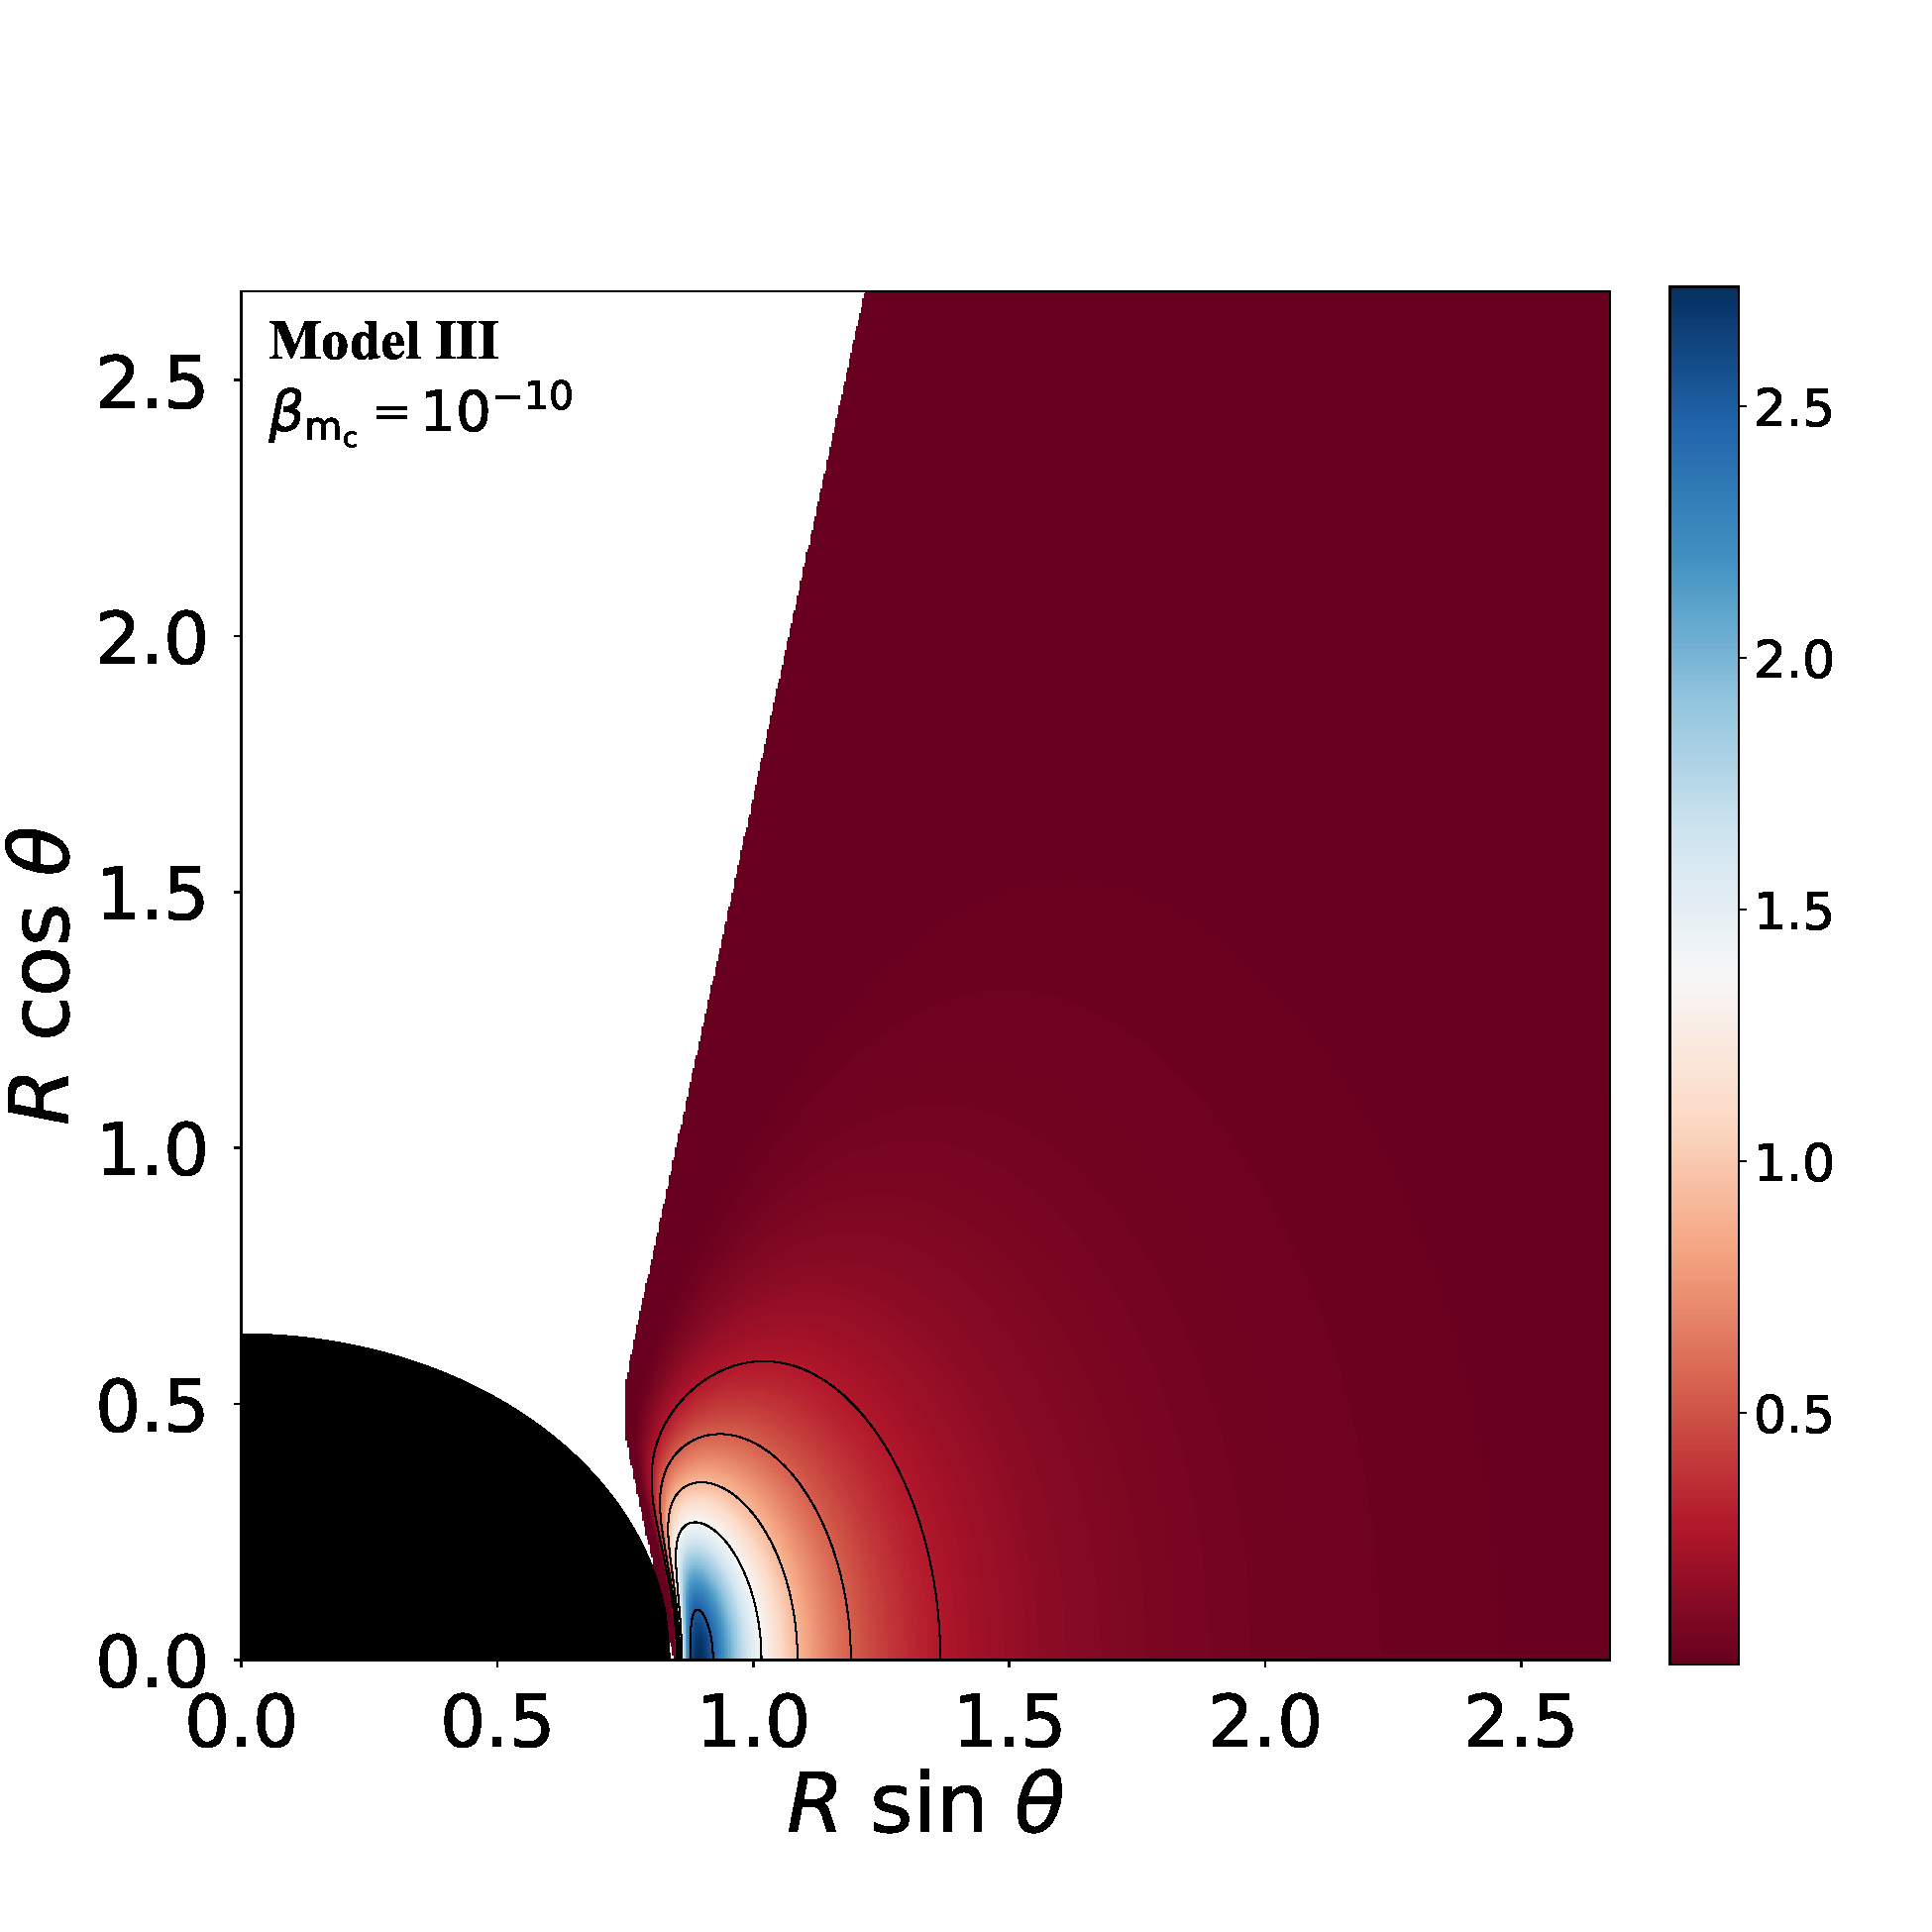
\includegraphics[scale=0.14]{figures/fig3_III__10.pdf}
\\
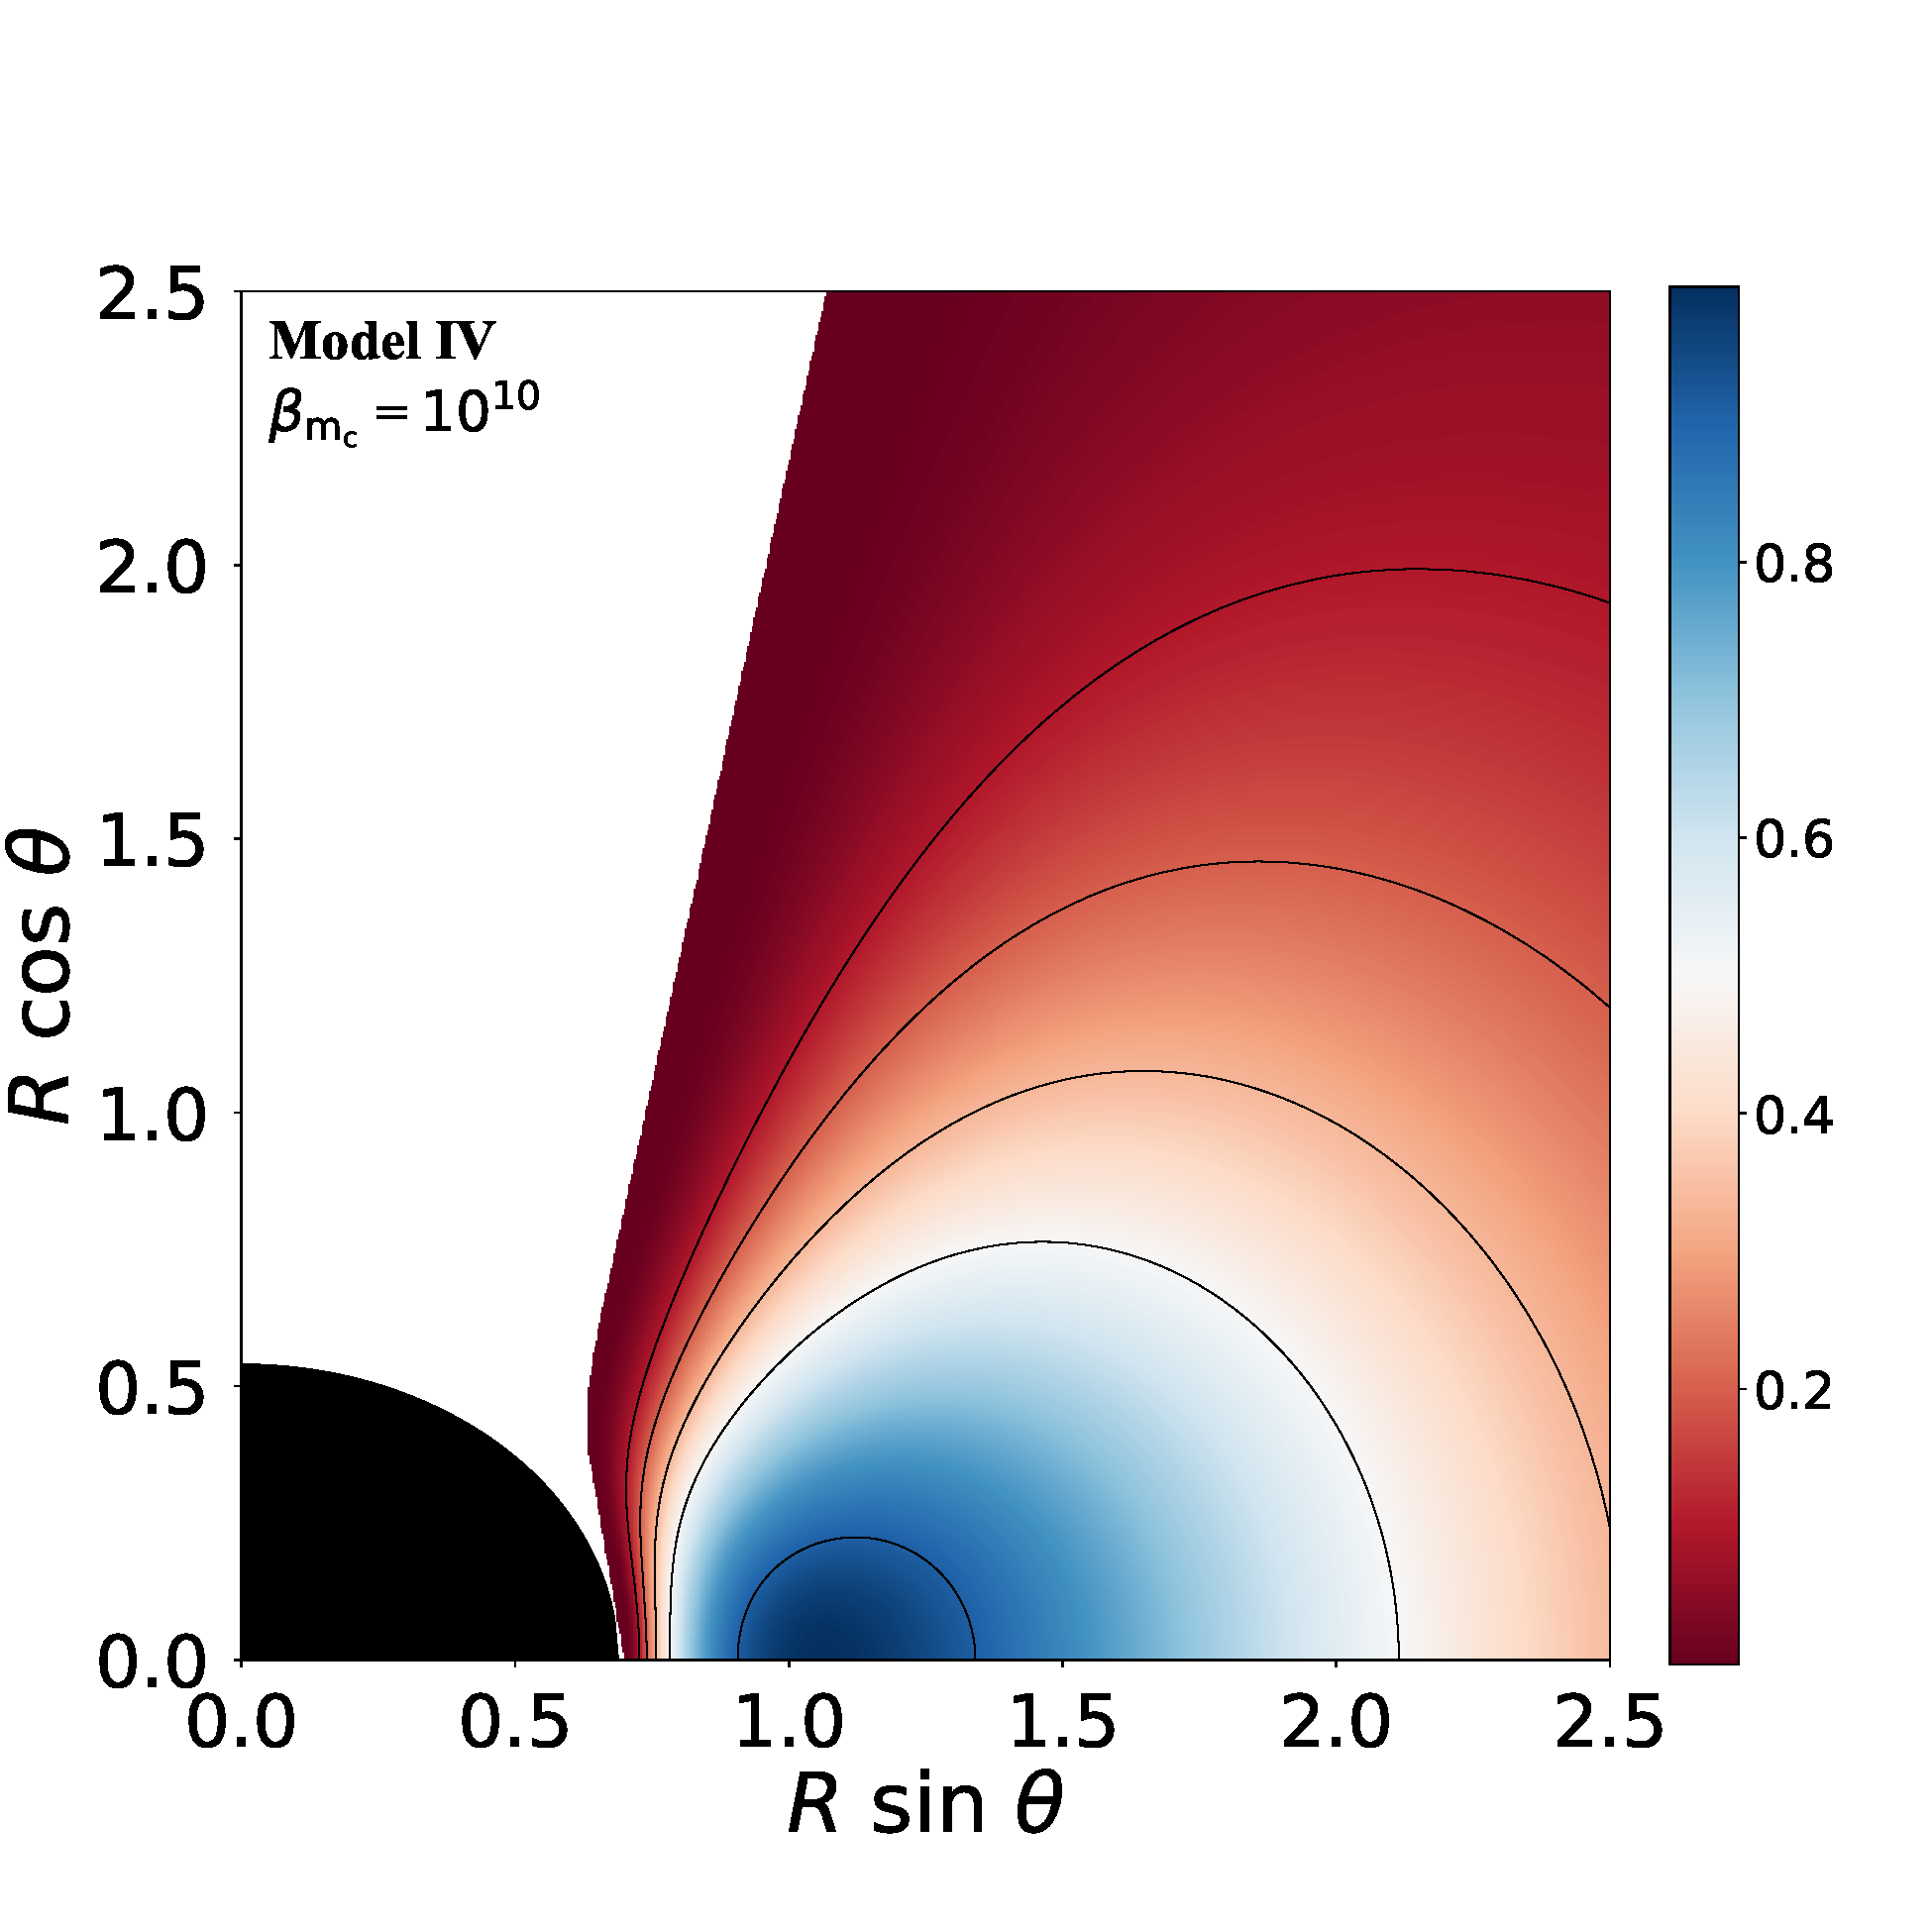
\includegraphics[scale=0.14]{figures/fig3_IV_10.pdf}
\hspace{-0.3cm}
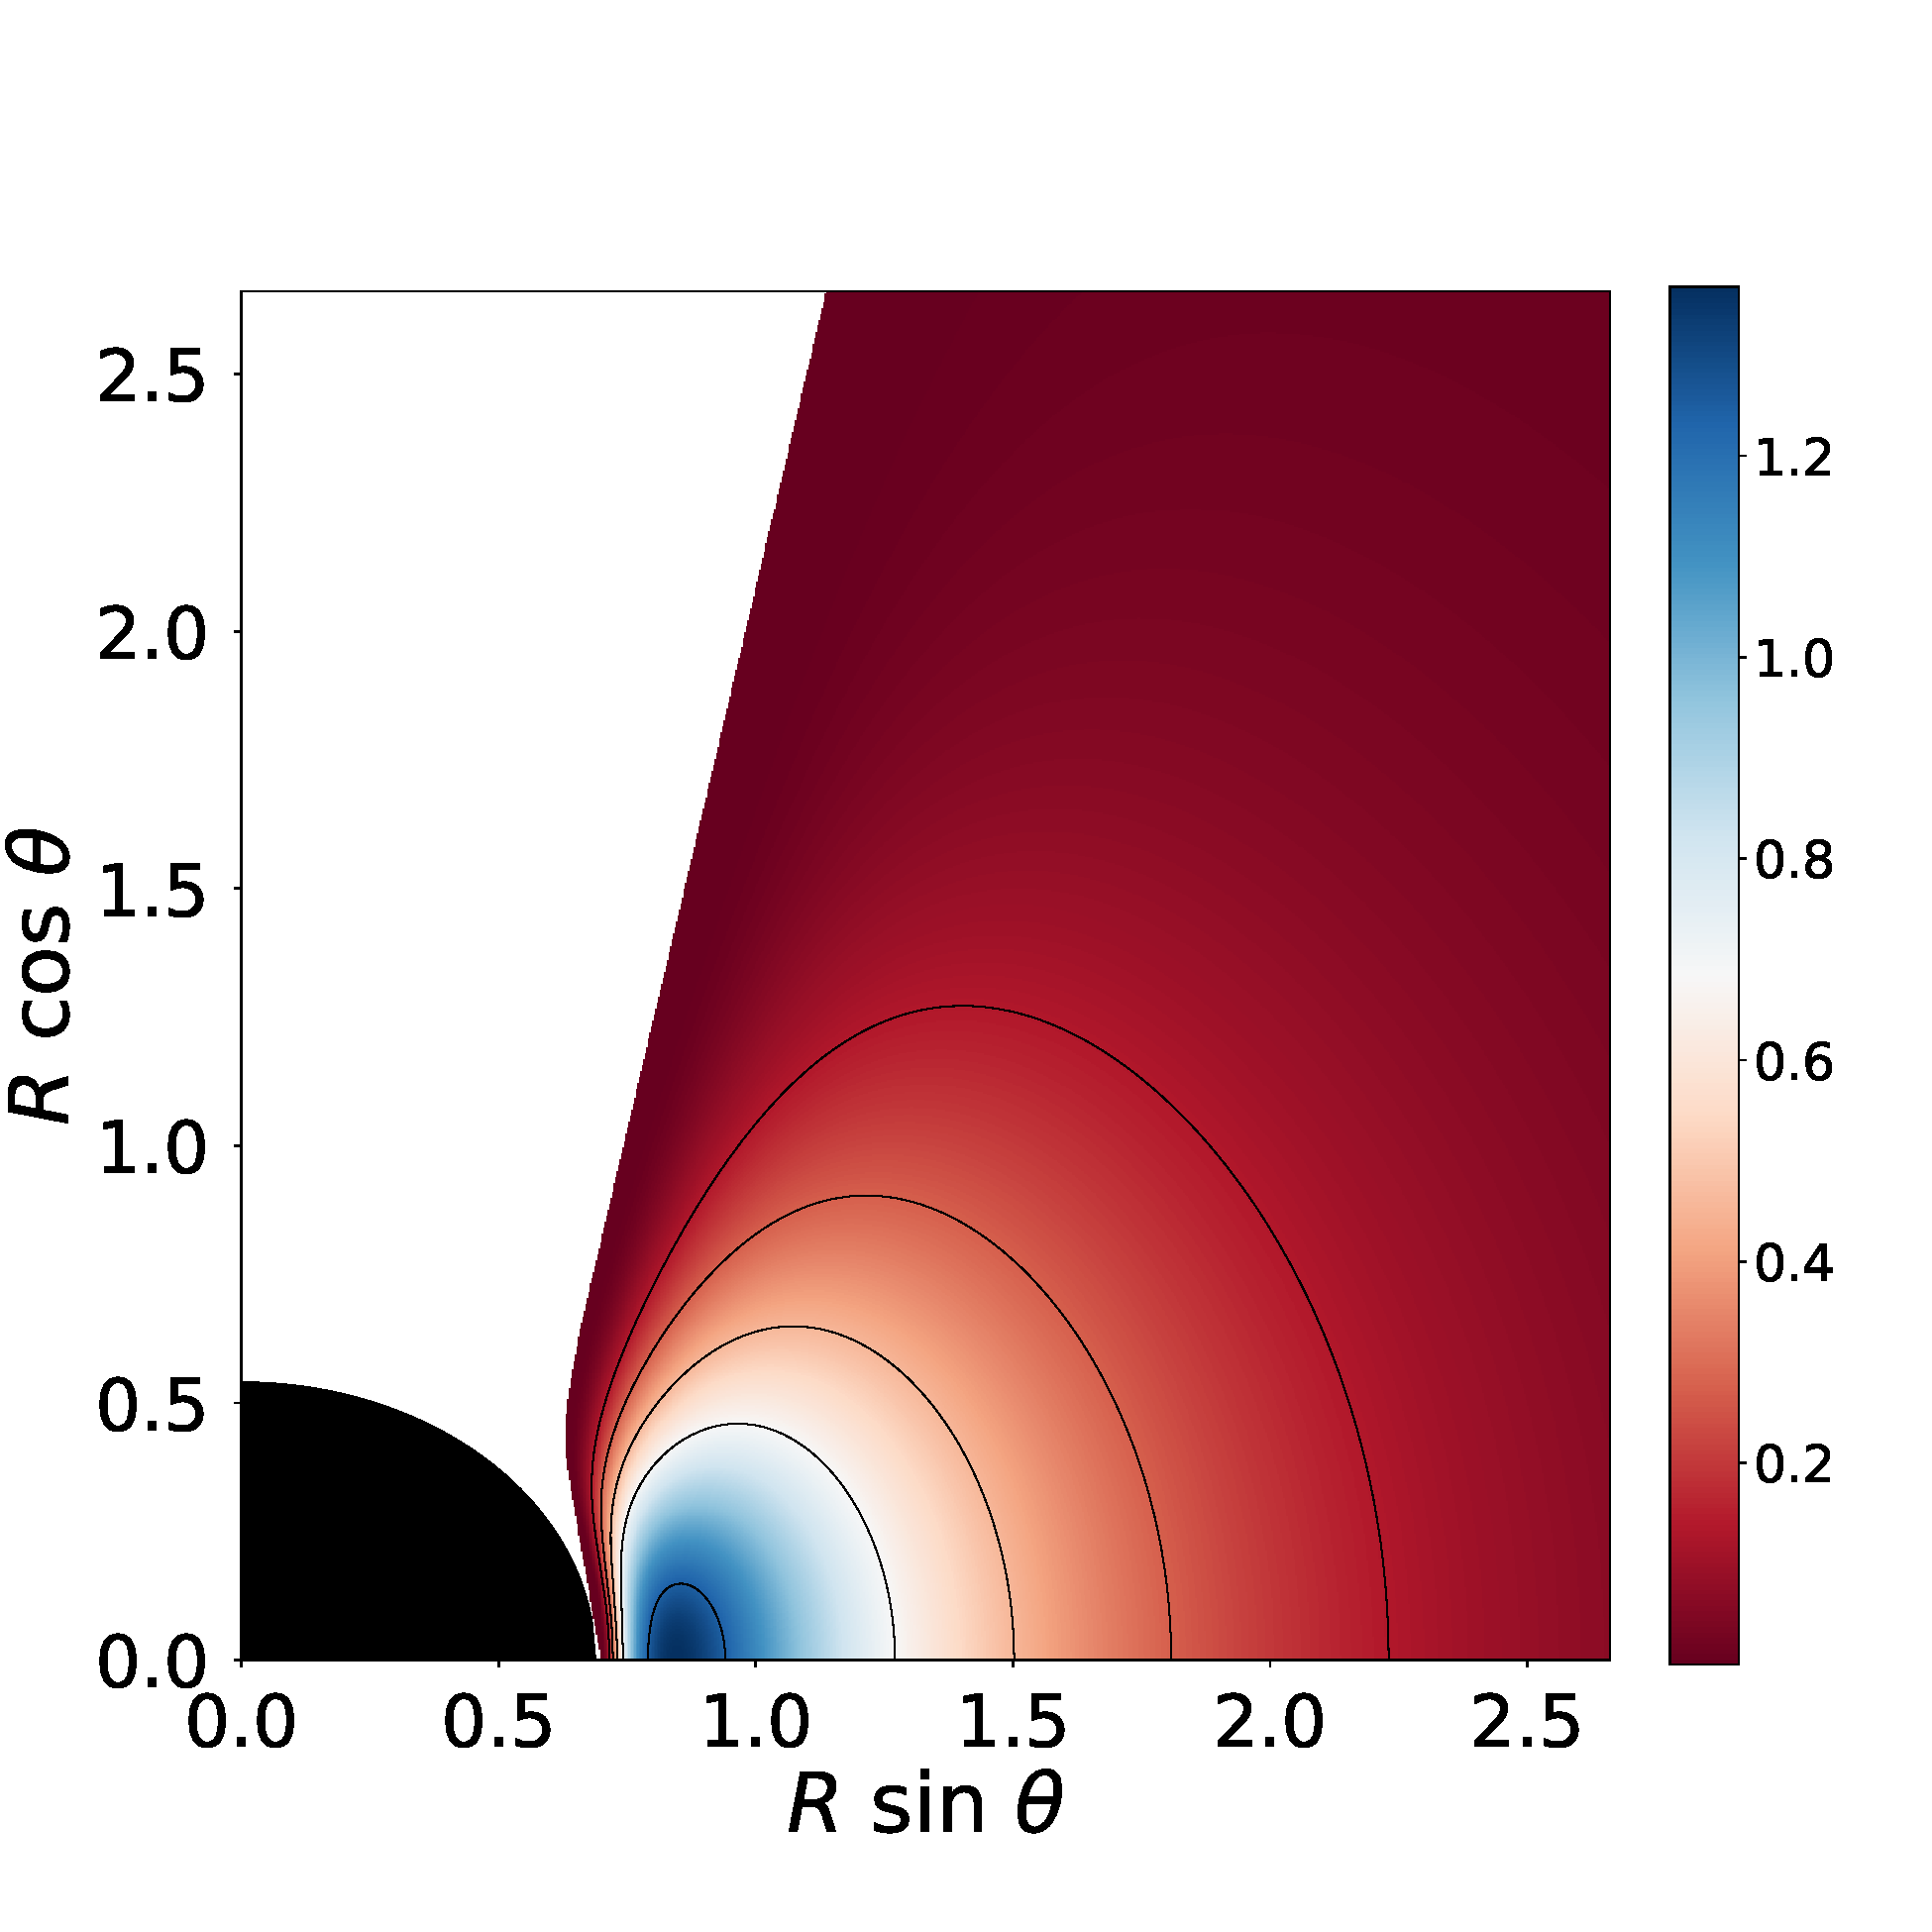
\includegraphics[scale=0.14]{figures/fig3_IV_1.pdf}
\hspace{-0.2cm}
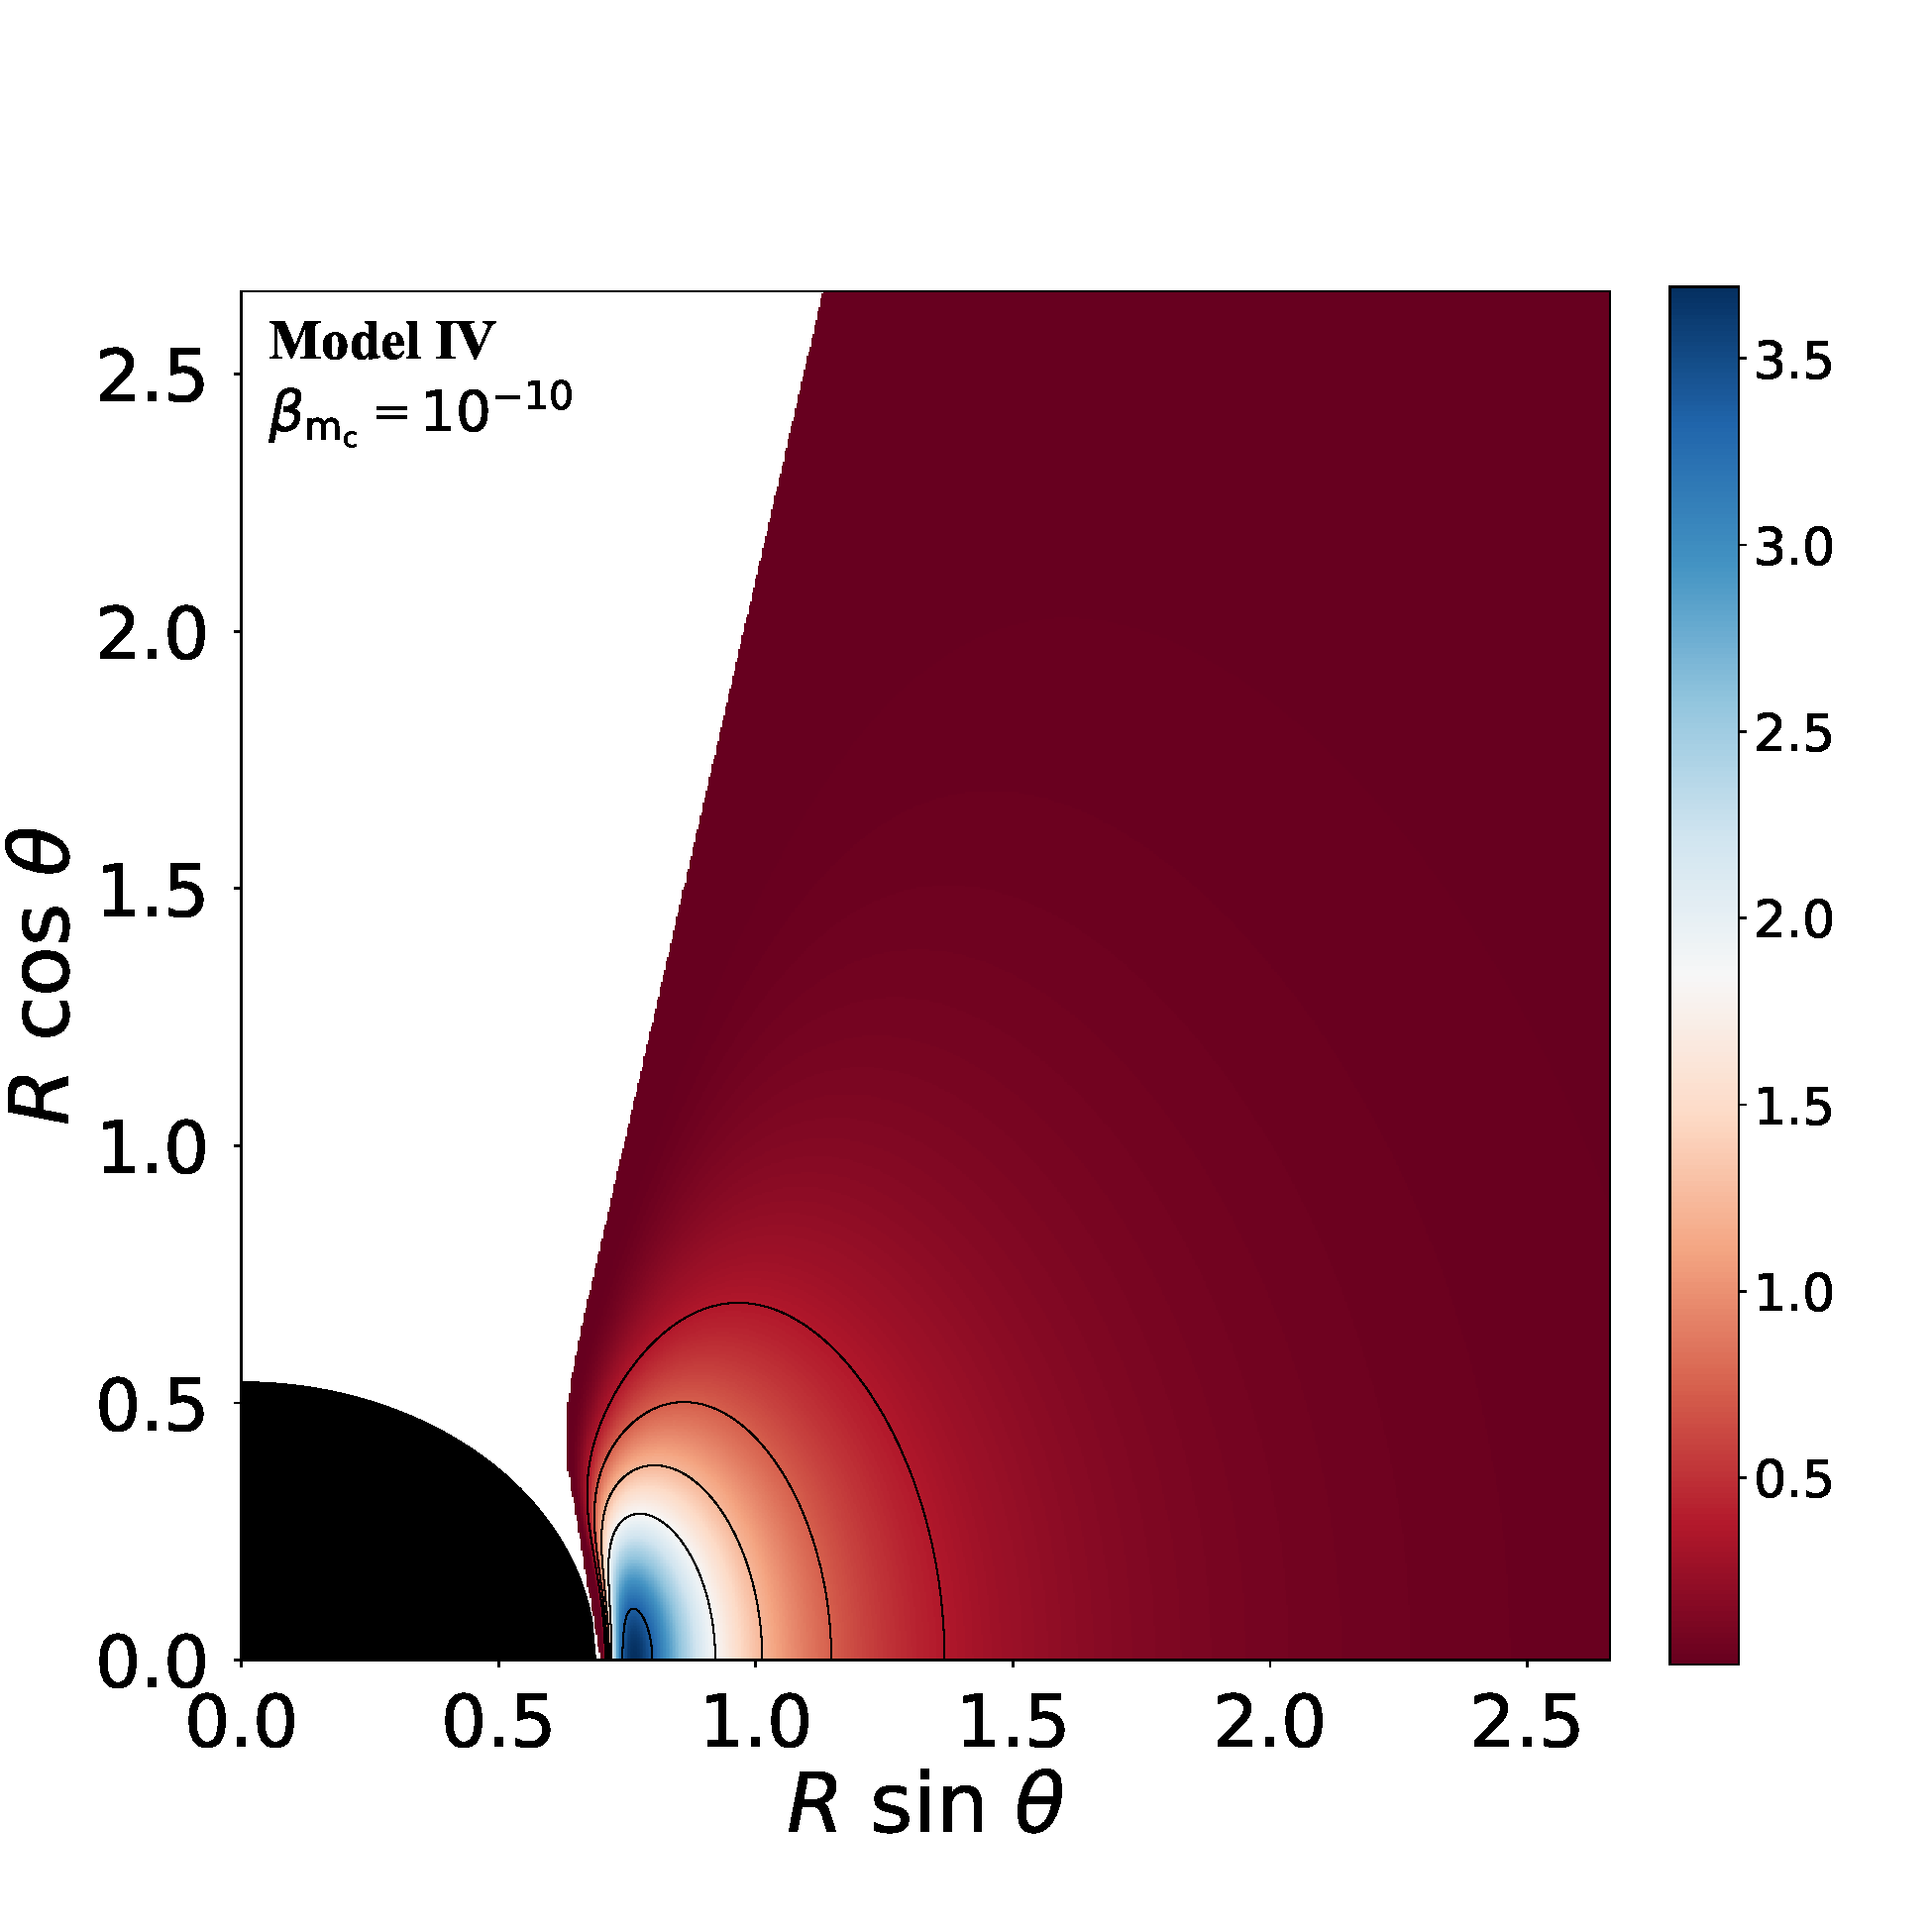
\includegraphics[scale=0.14]{figures/fig3_IV__10.pdf}
\hspace{-0.2cm}
\caption{Rest-mass density distribution using perimeteral coordinates. From top to bottom the rows correspond to the different models for the KBHsSH (I, II, III and IV). From left to right the columns correspond to different values of the magnetization parameter, namely non-magnetized ($\beta_{\mathrm{m}_{\mathrm{c}}} = 10^{10}$), mildly magnetized ($\beta_{\mathrm{m}_{\mathrm{c}}} = 1$) and strongly magnetized ($\beta_{\mathrm{m}_{\mathrm{c}}} = 10^{-10}$)}
\label{models_peri_I}
\end{figure*}

\begin{figure*}
\centering
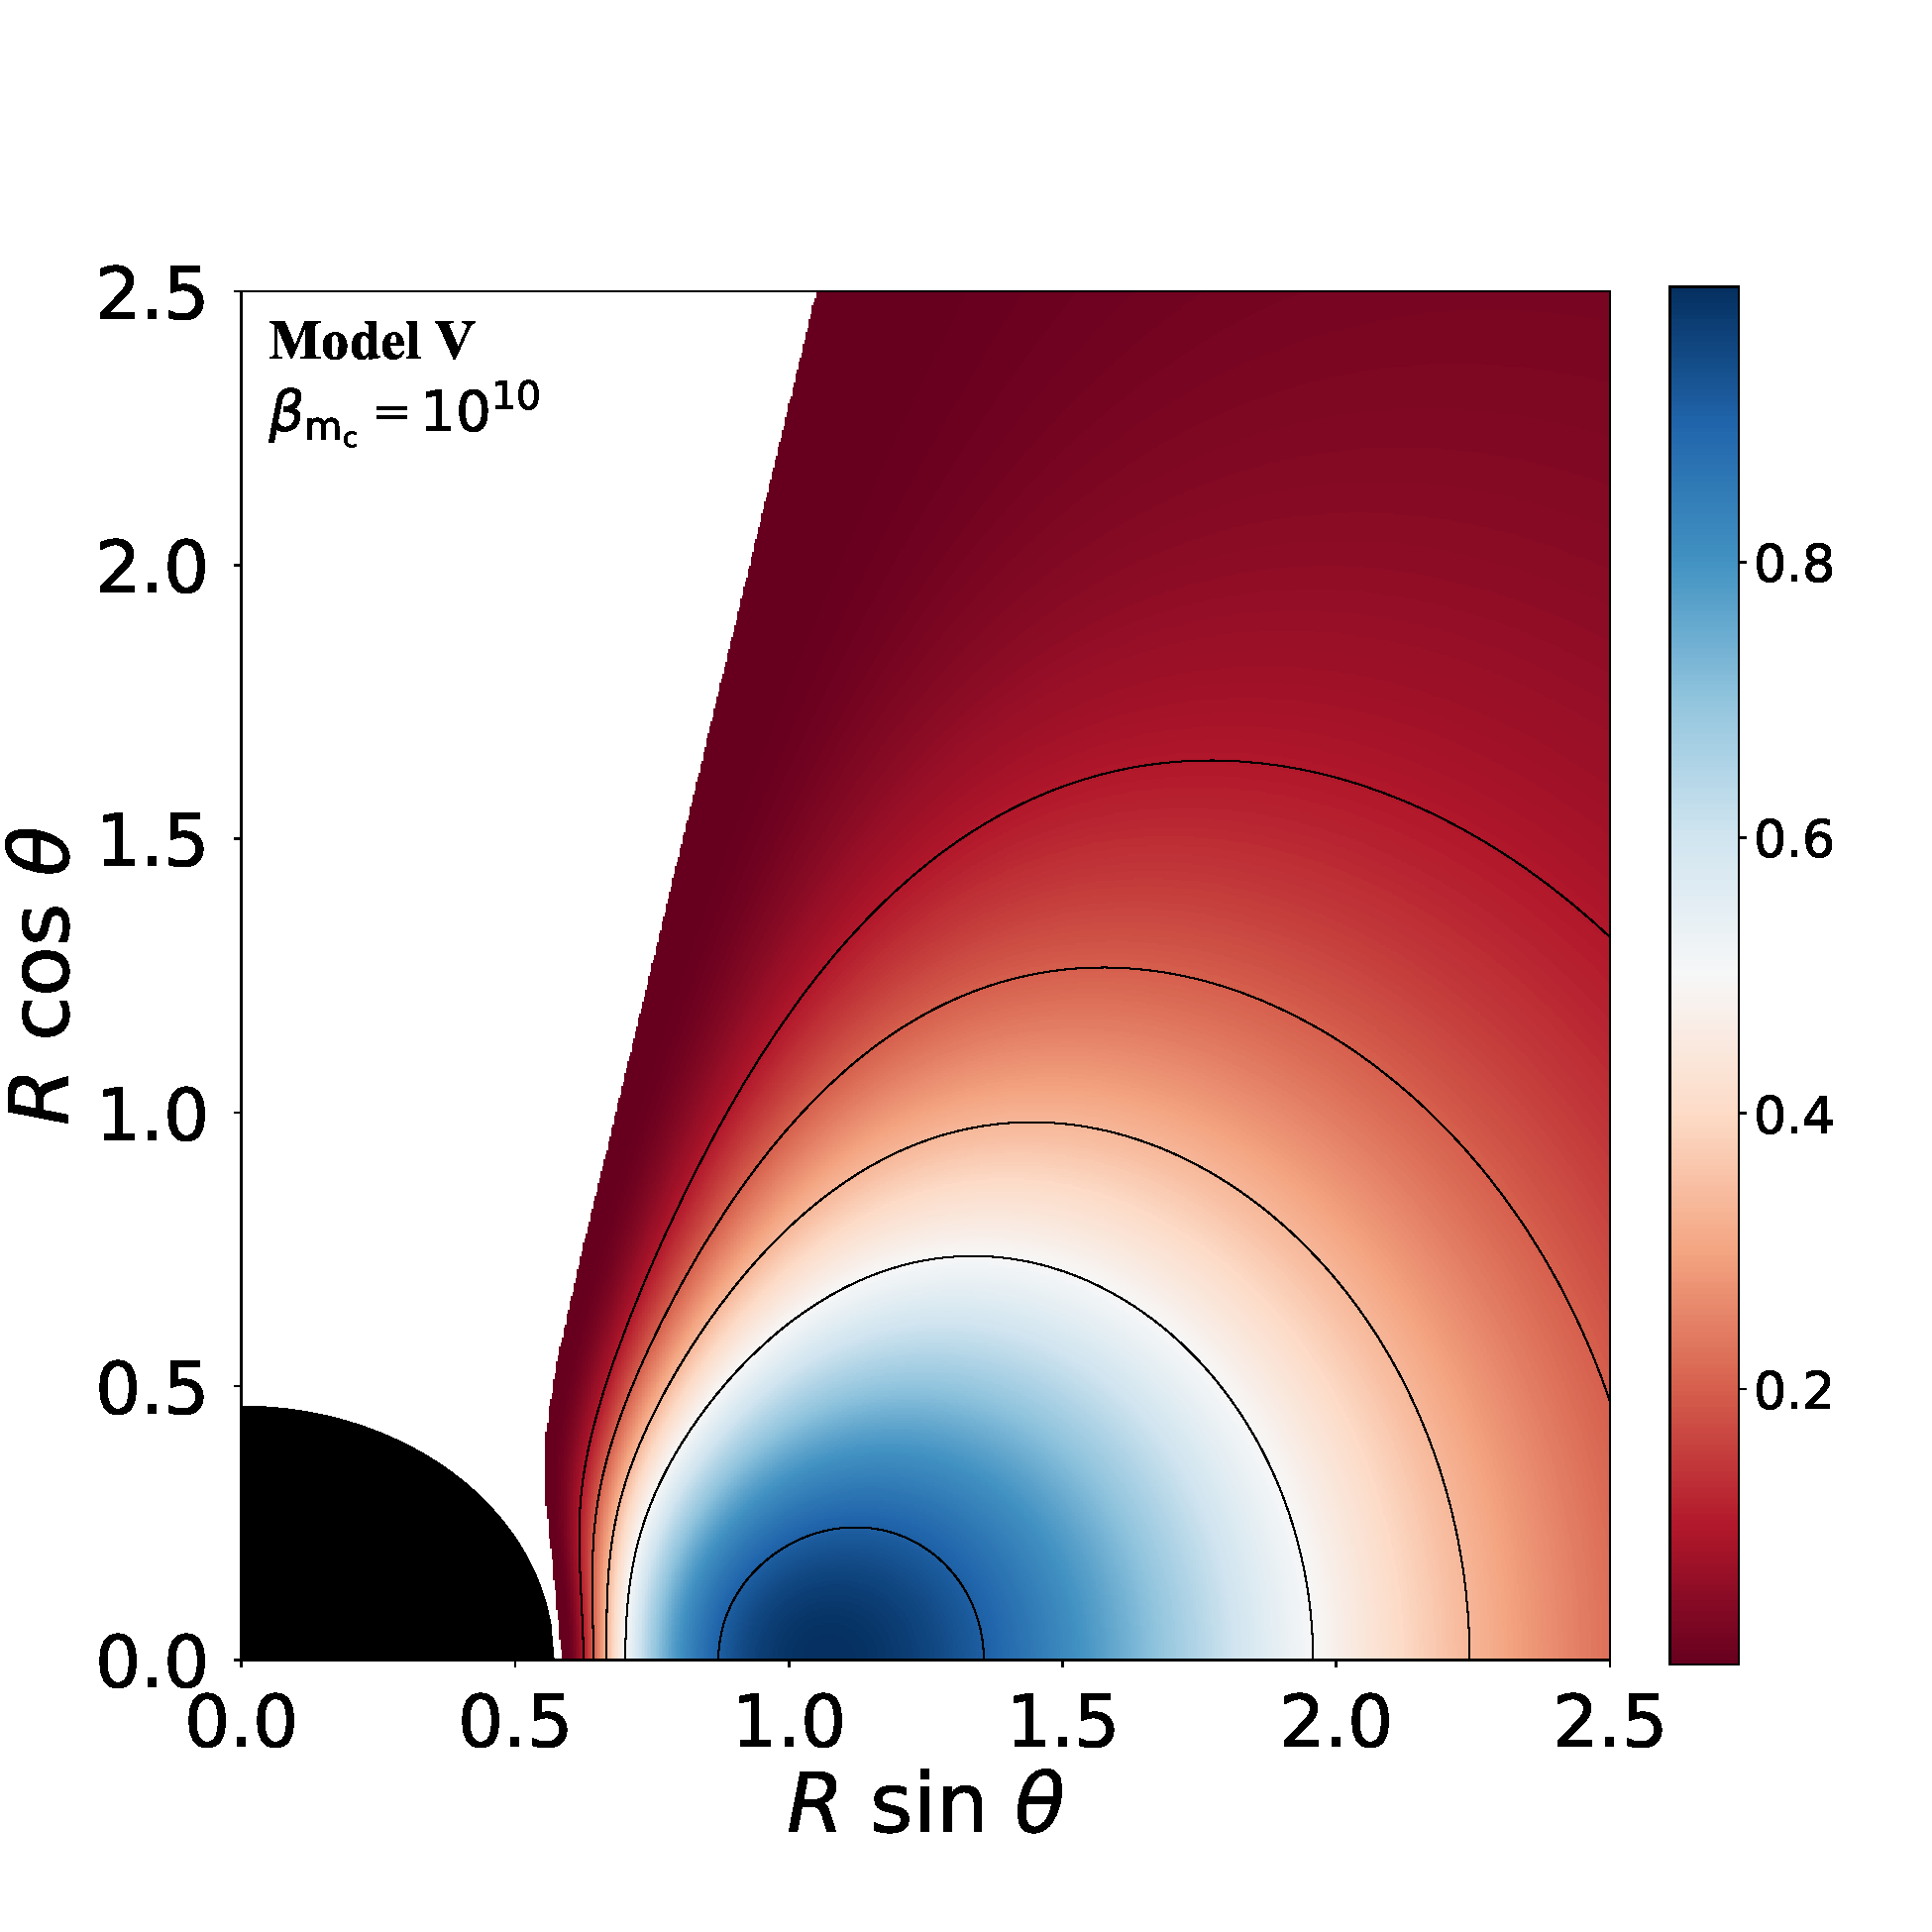
\includegraphics[scale=0.14]{figures/fig4_V_10.pdf}
\hspace{-0.3cm}
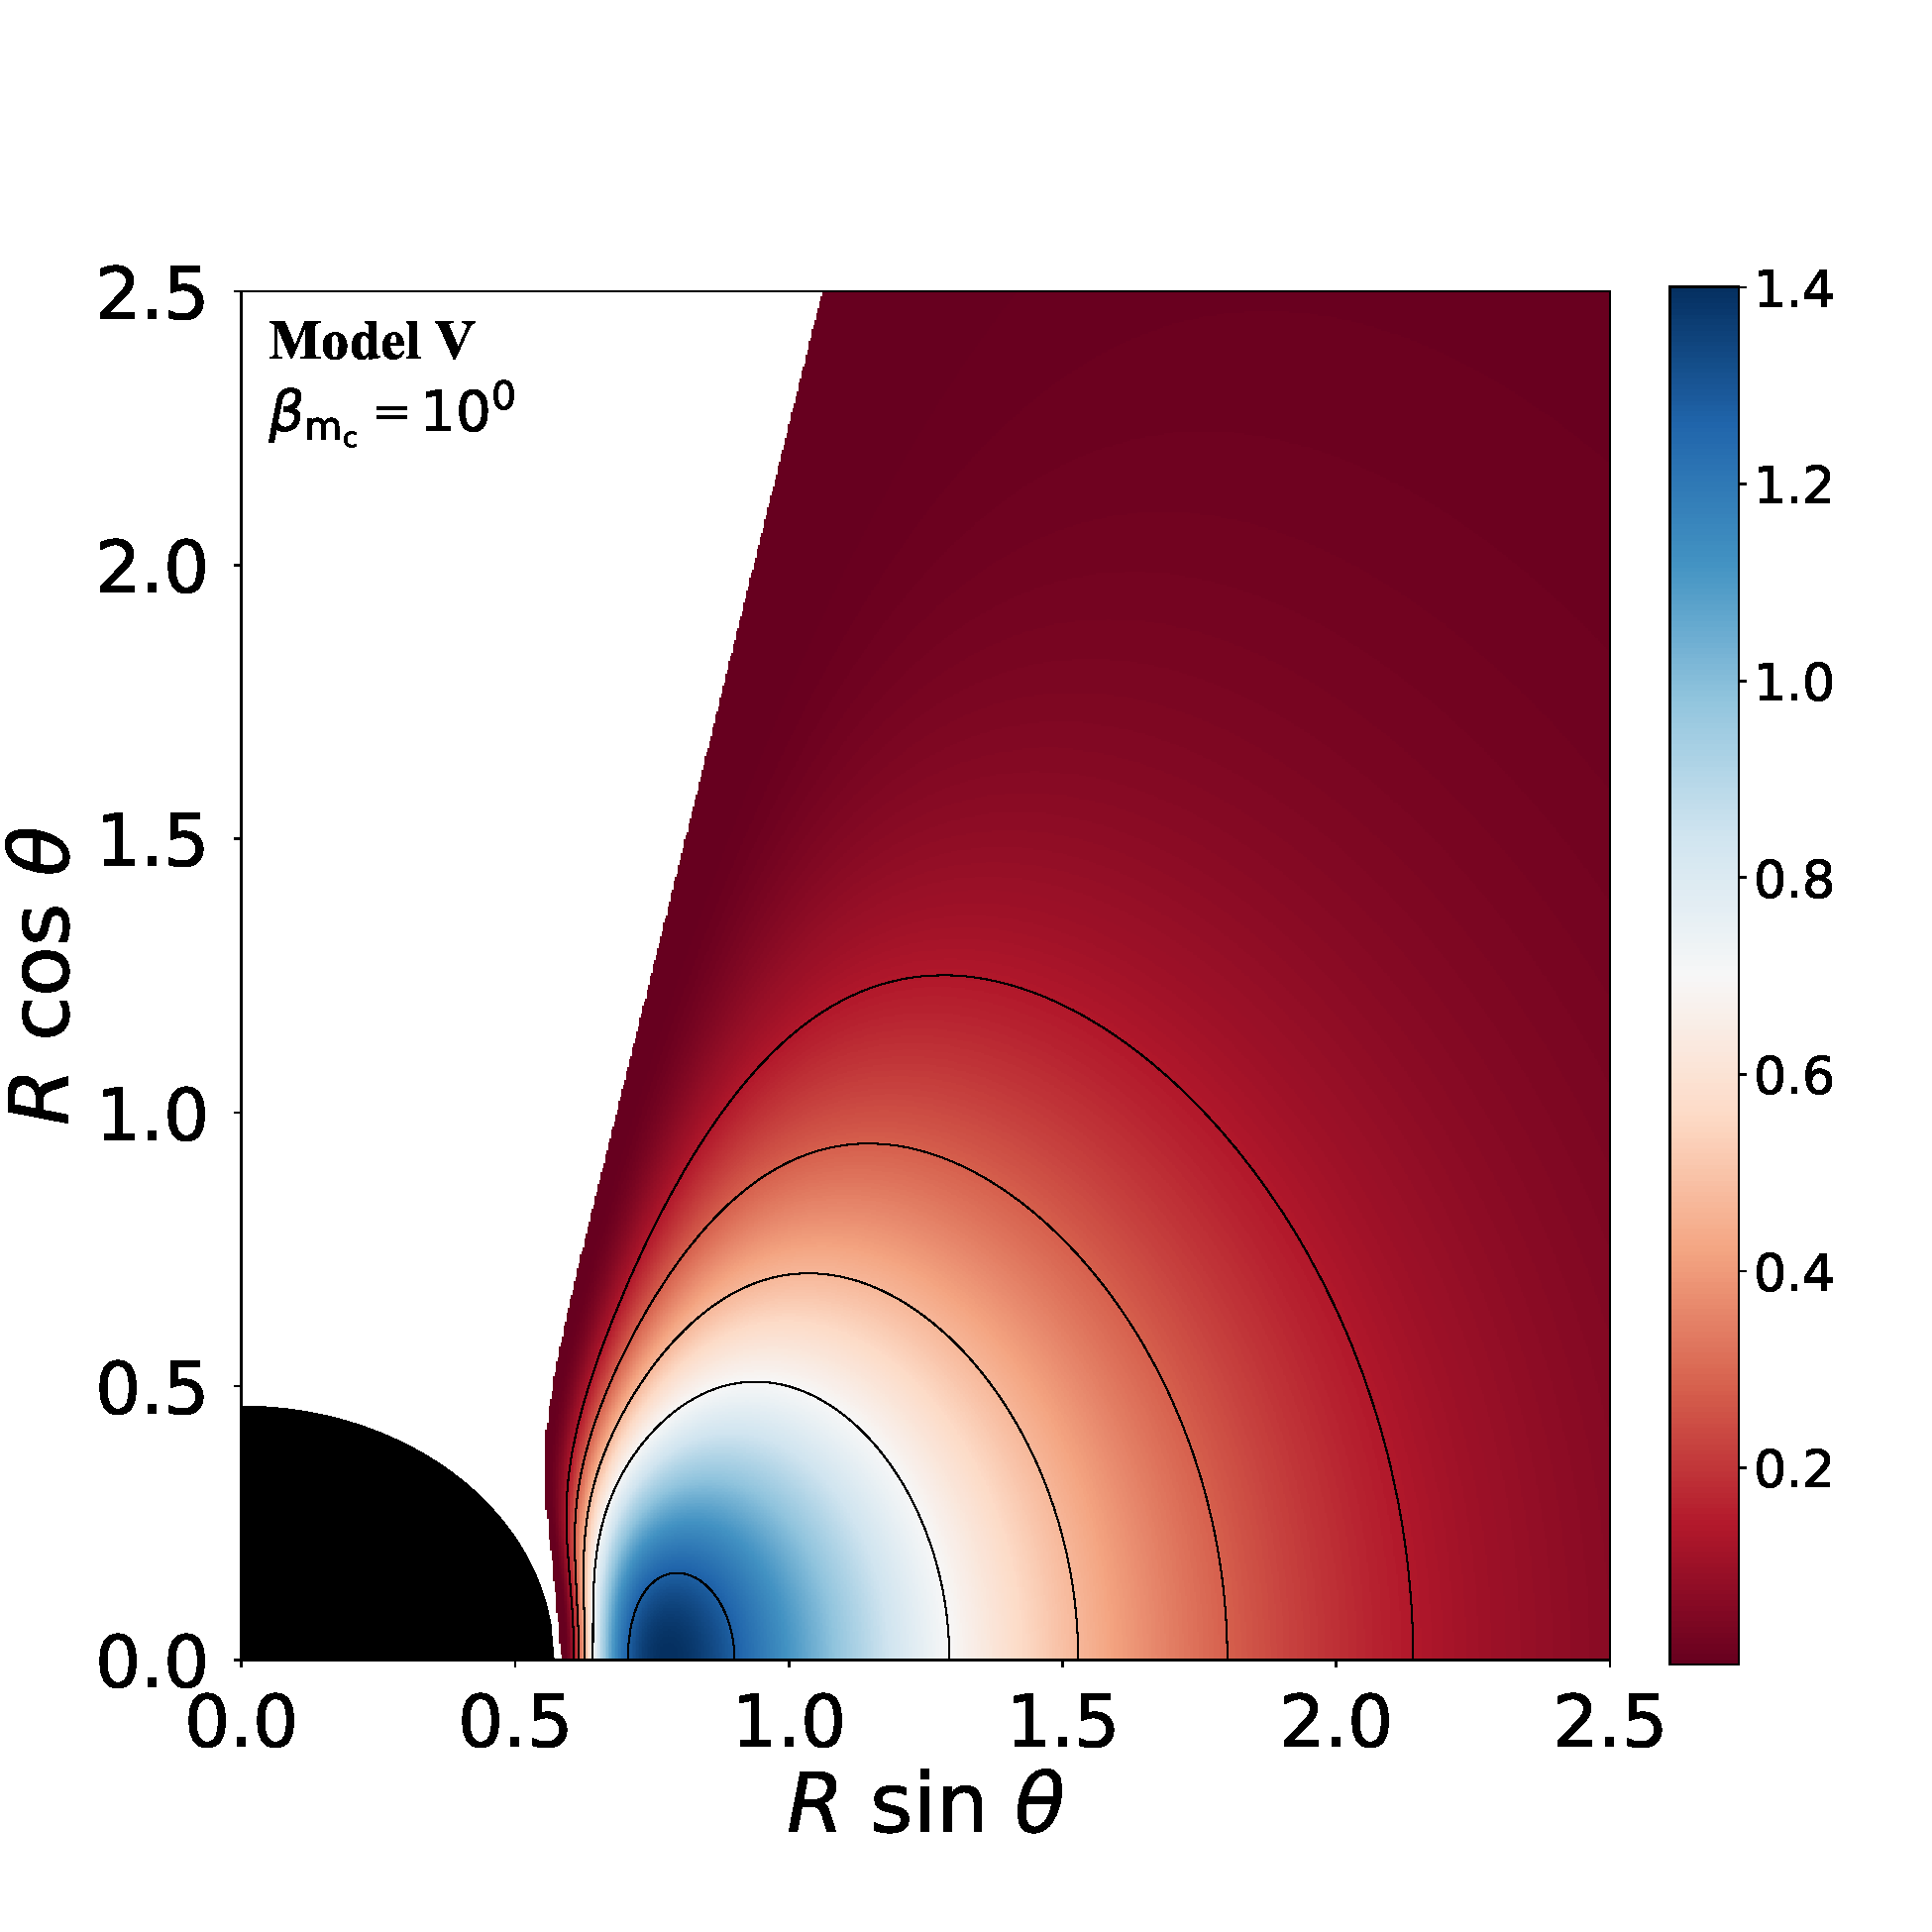
\includegraphics[scale=0.14]{figures/fig4_V_1.pdf}
\hspace{-0.2cm}
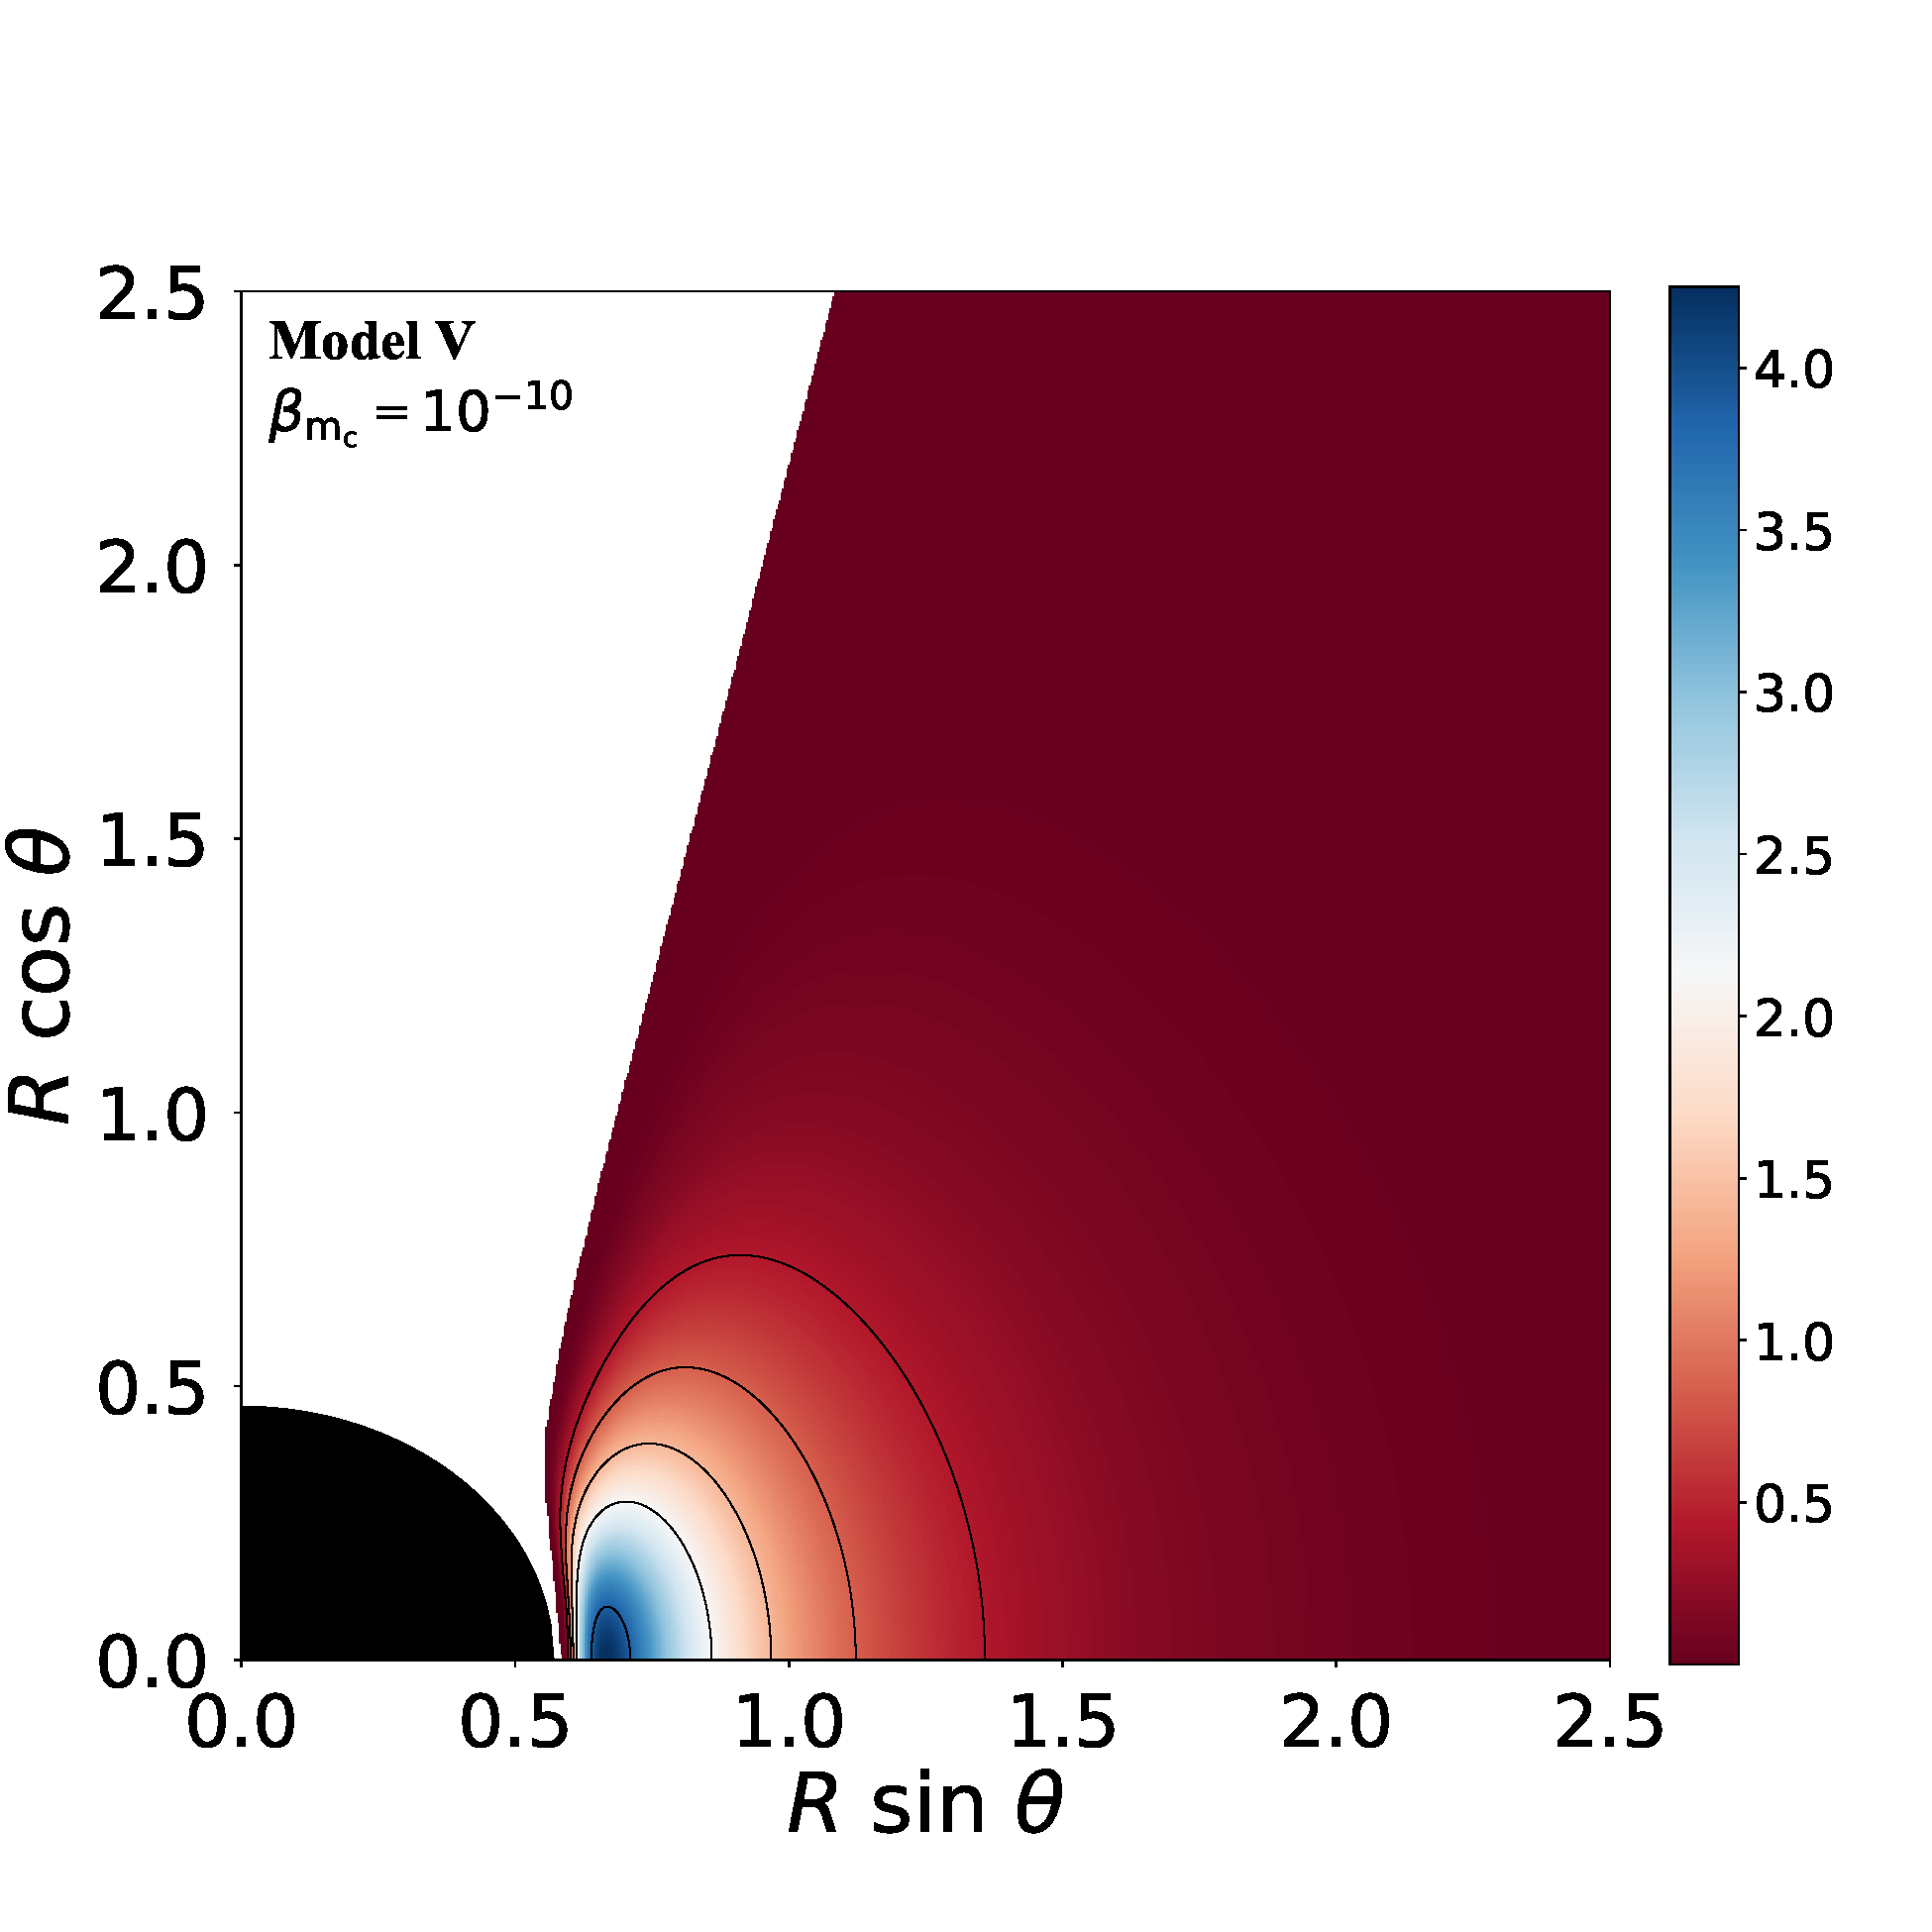
\includegraphics[scale=0.14]{figures/fig4_V__10.pdf}
\\
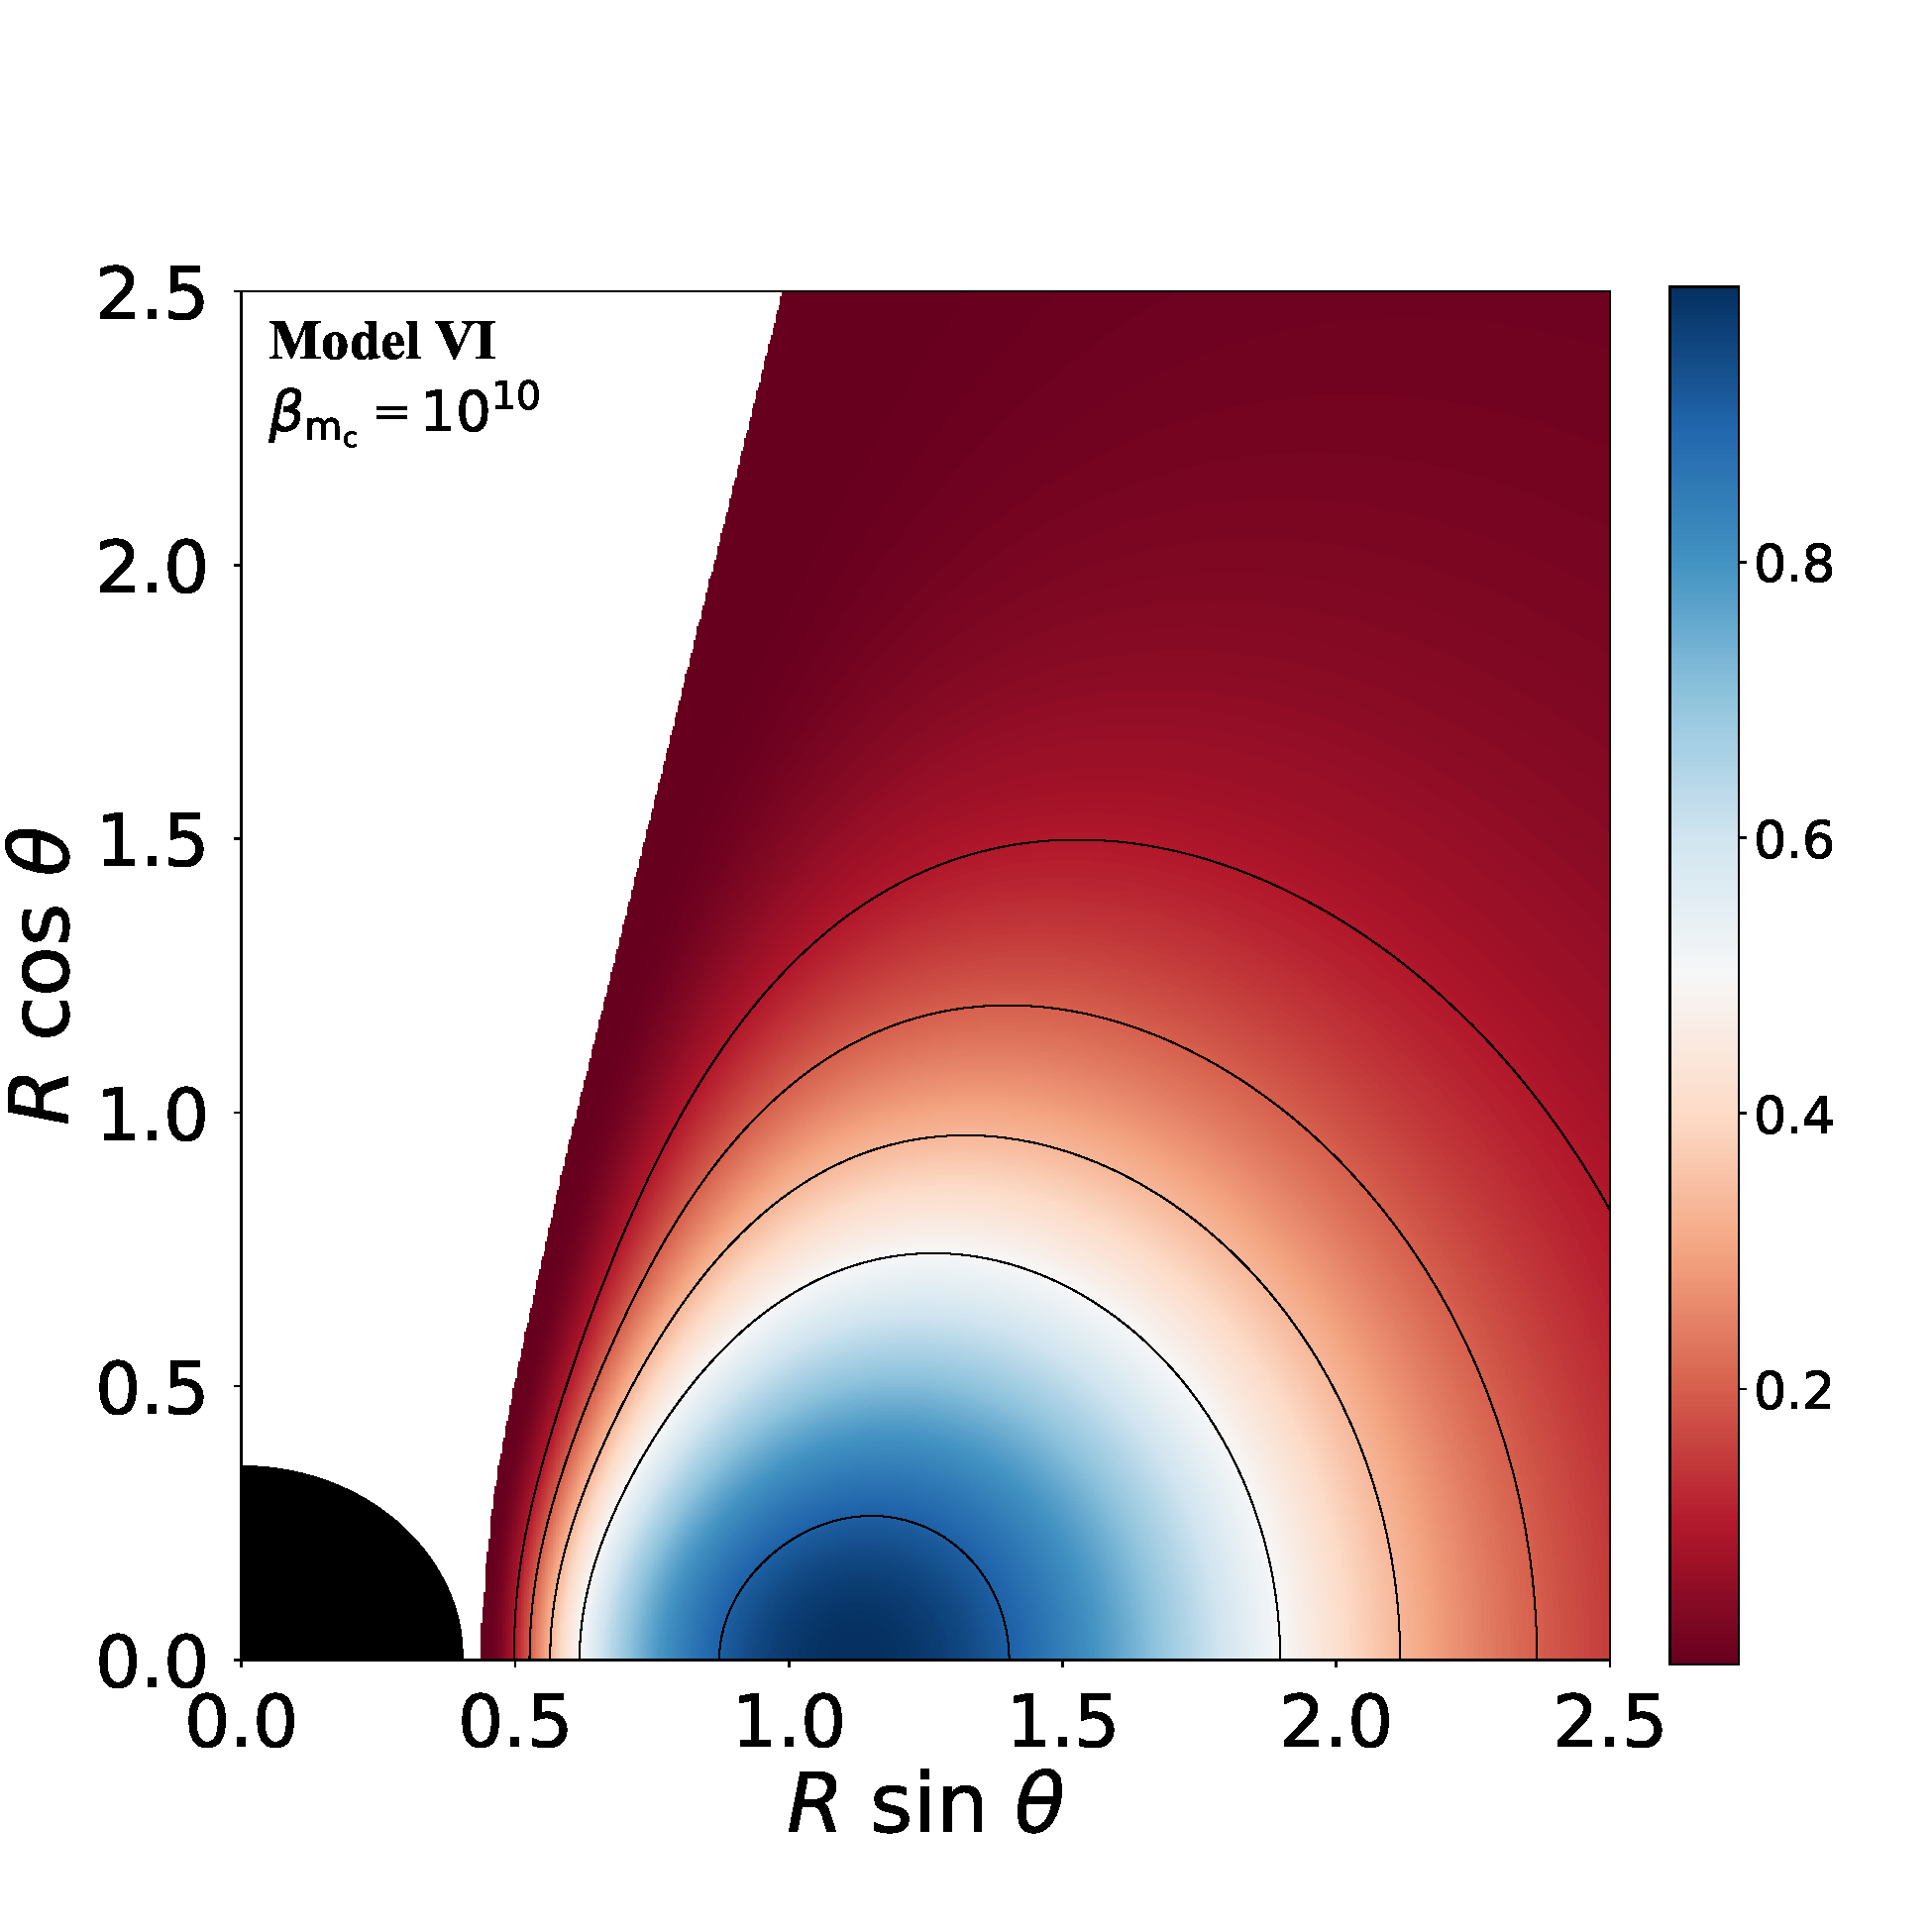
\includegraphics[scale=0.14]{figures/fig4_VI_10.pdf}
\hspace{-0.3cm}
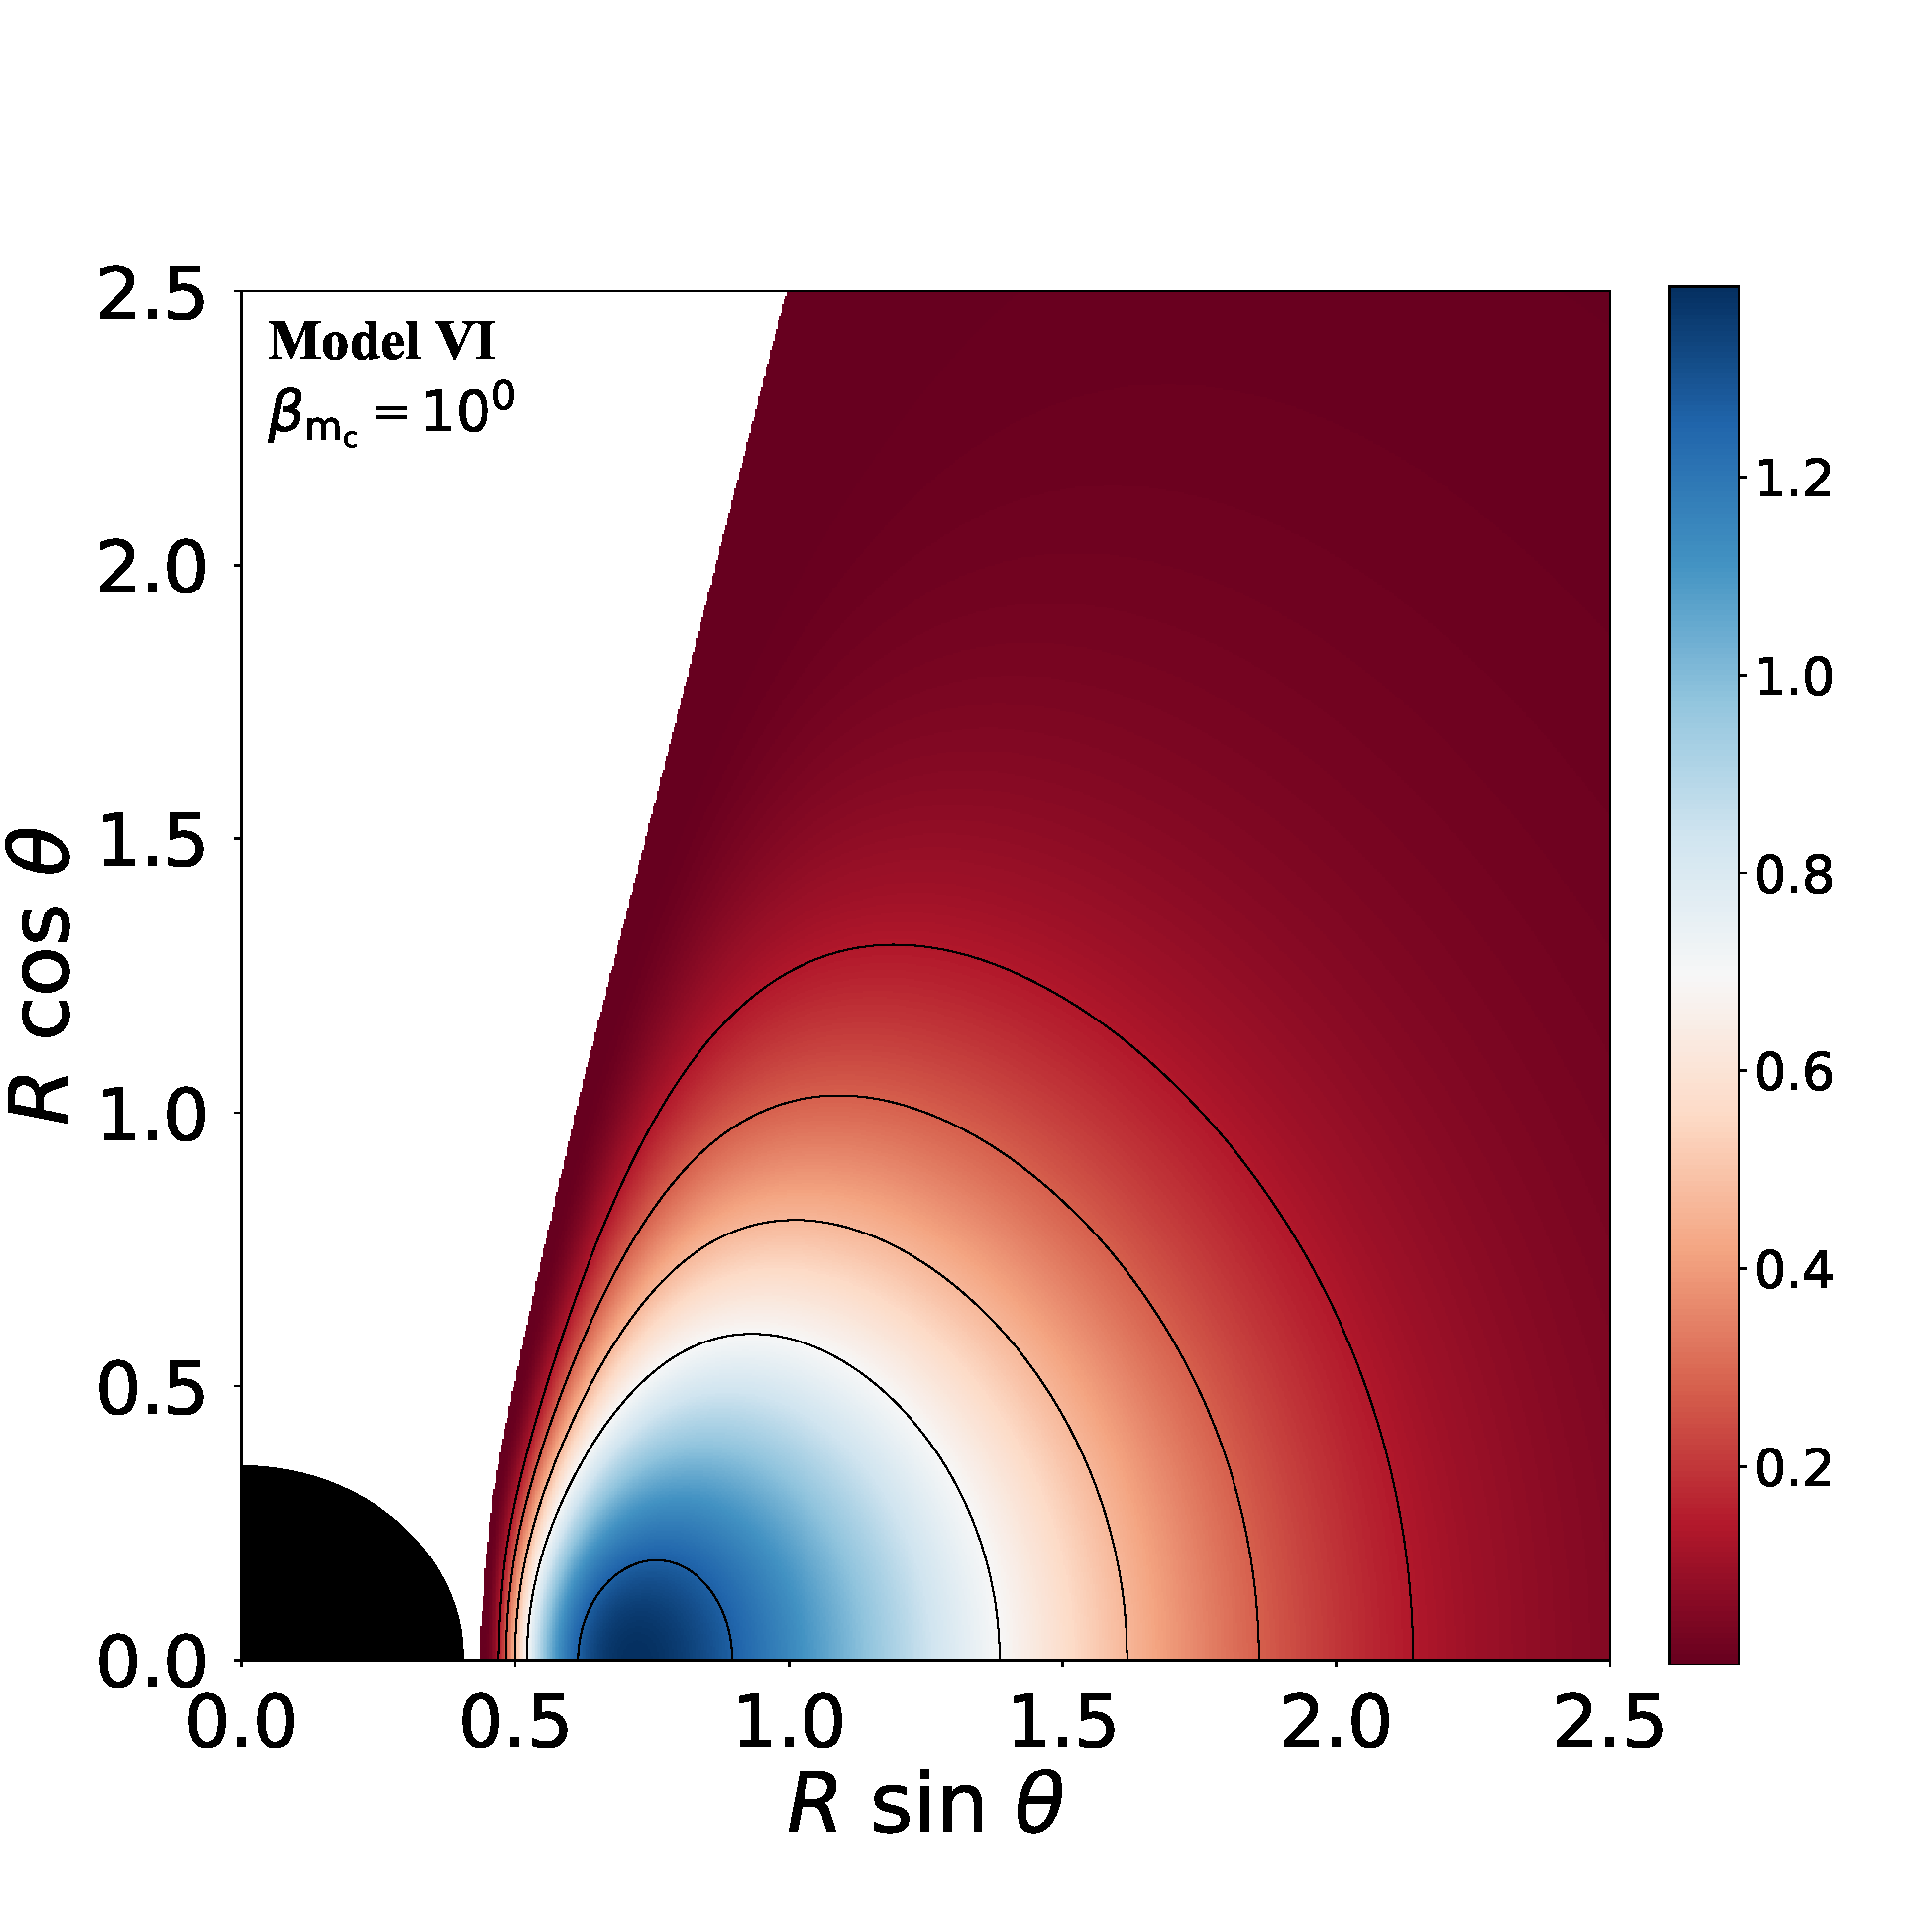
\includegraphics[scale=0.14]{figures/fig4_VI_1.pdf}
\hspace{-0.2cm}
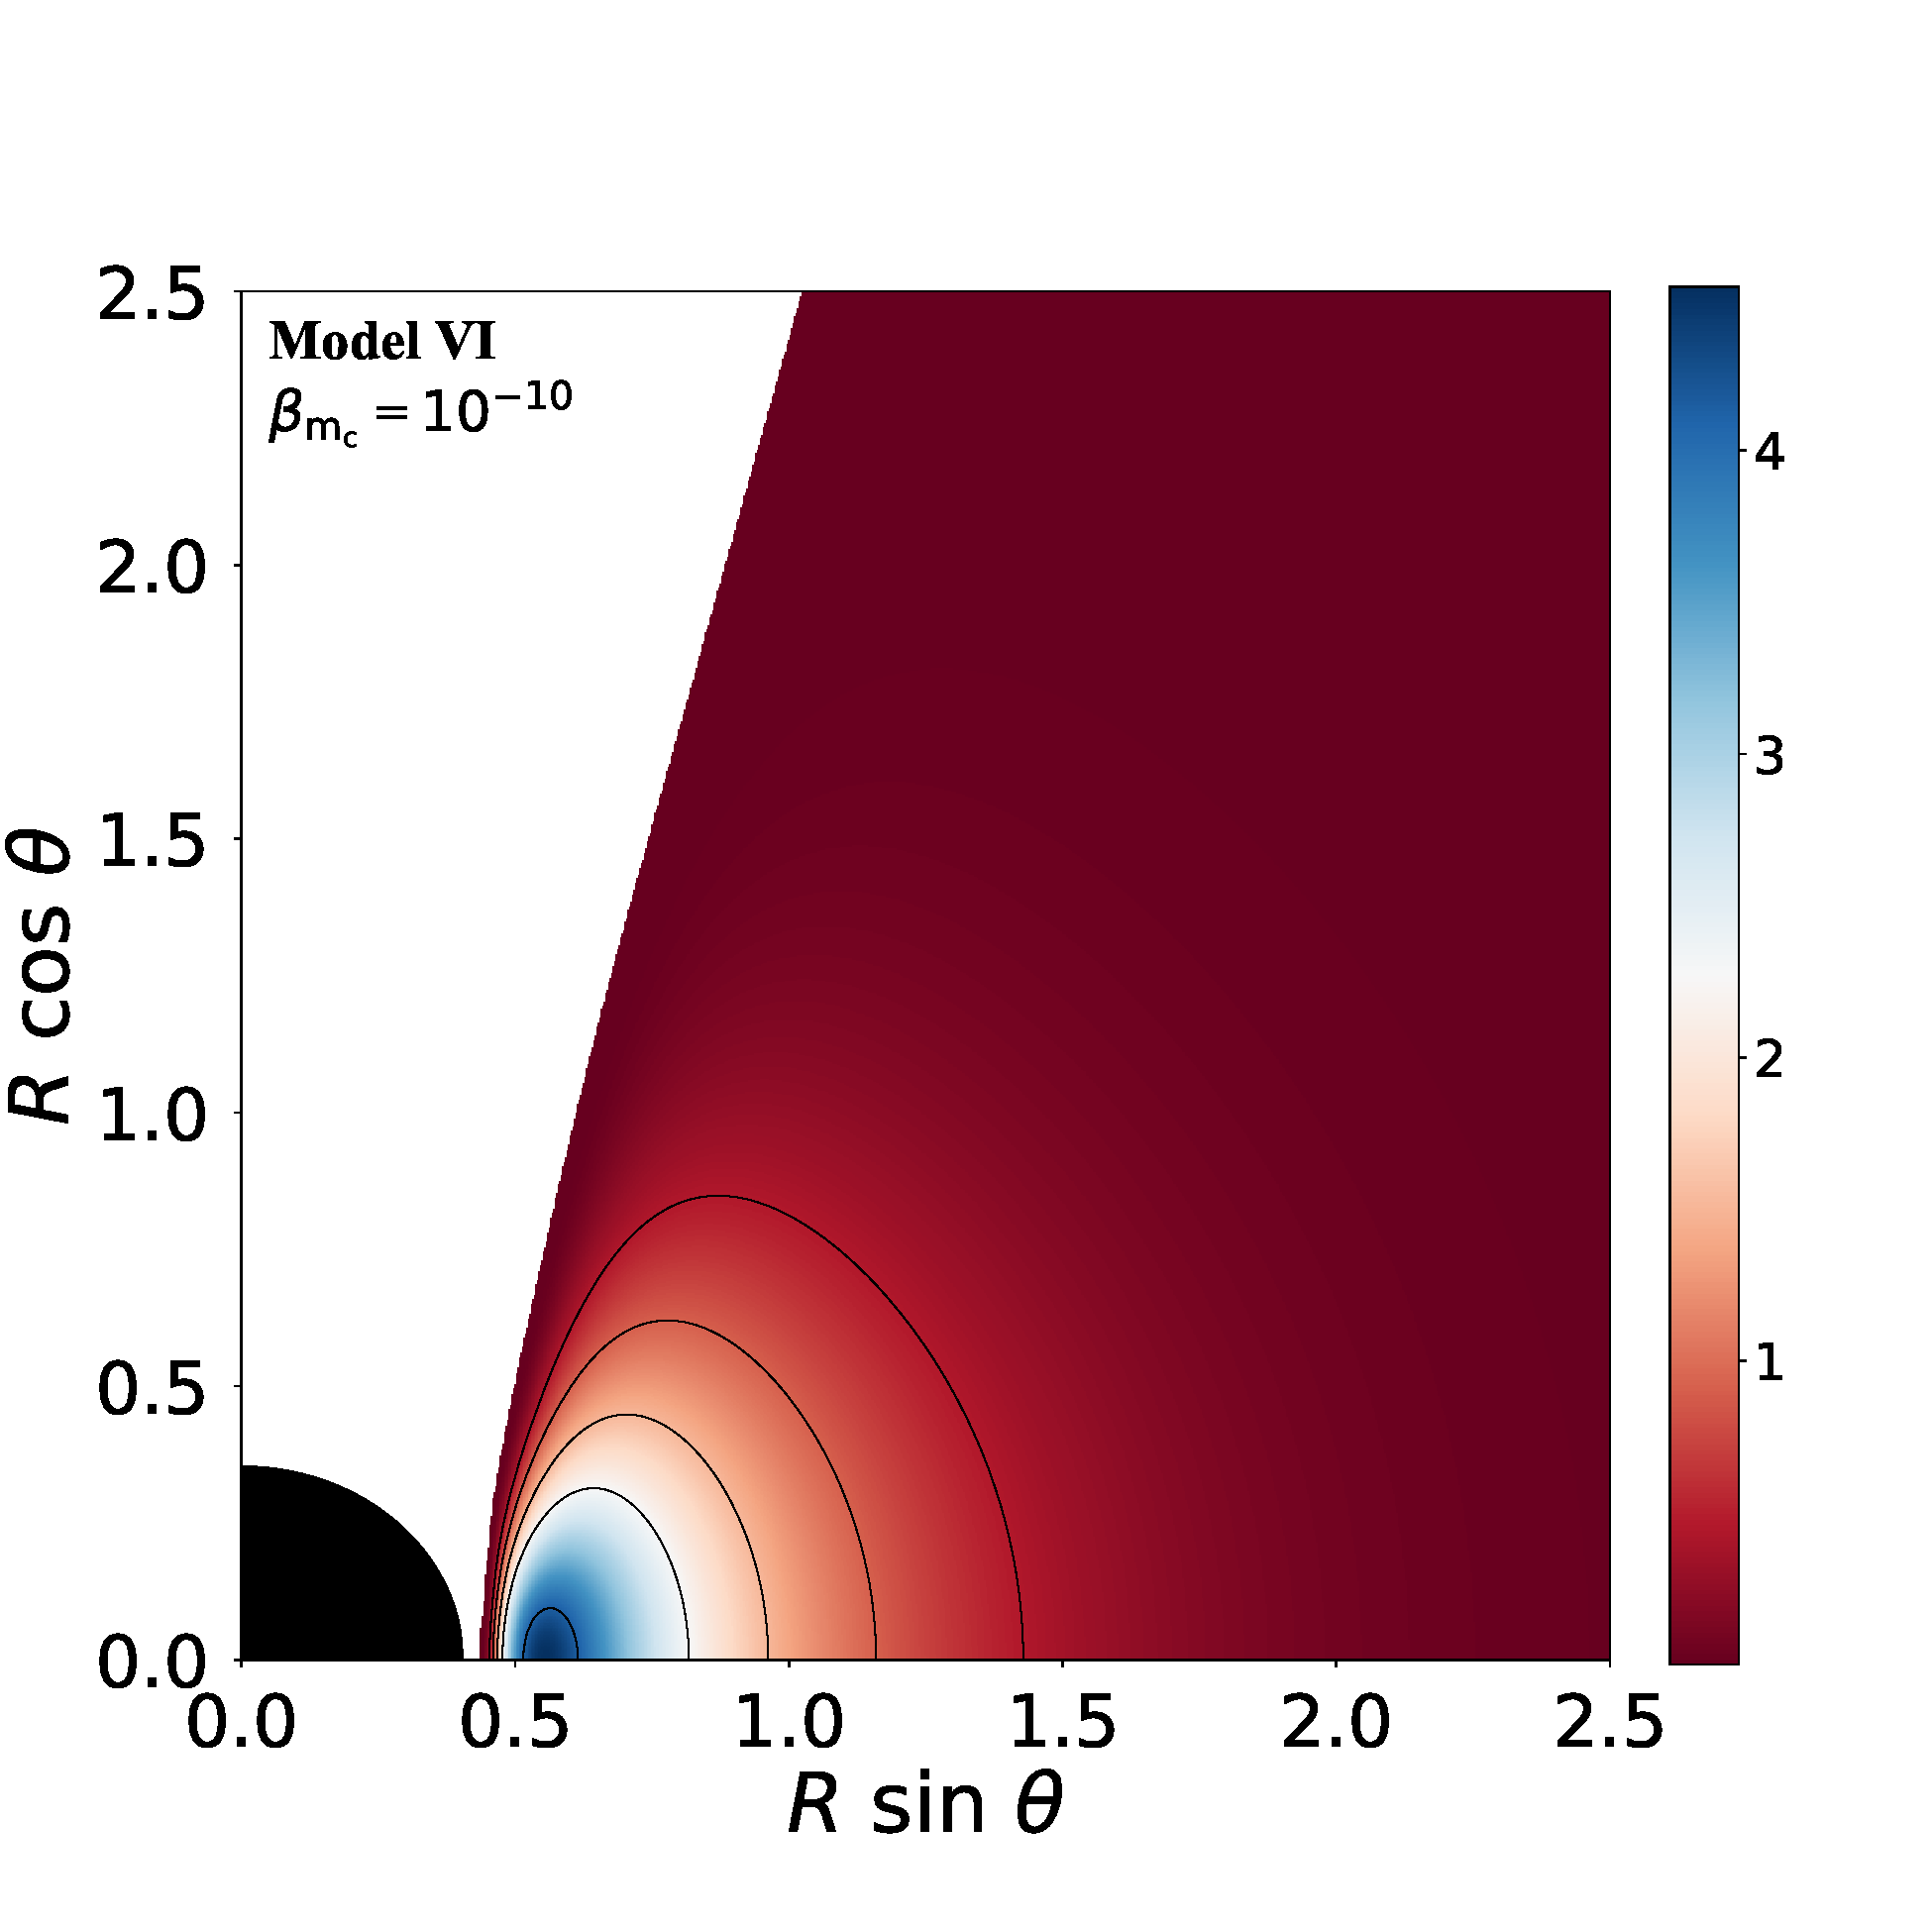
\includegraphics[scale=0.14]{figures/fig4_VI__10.pdf}
\\
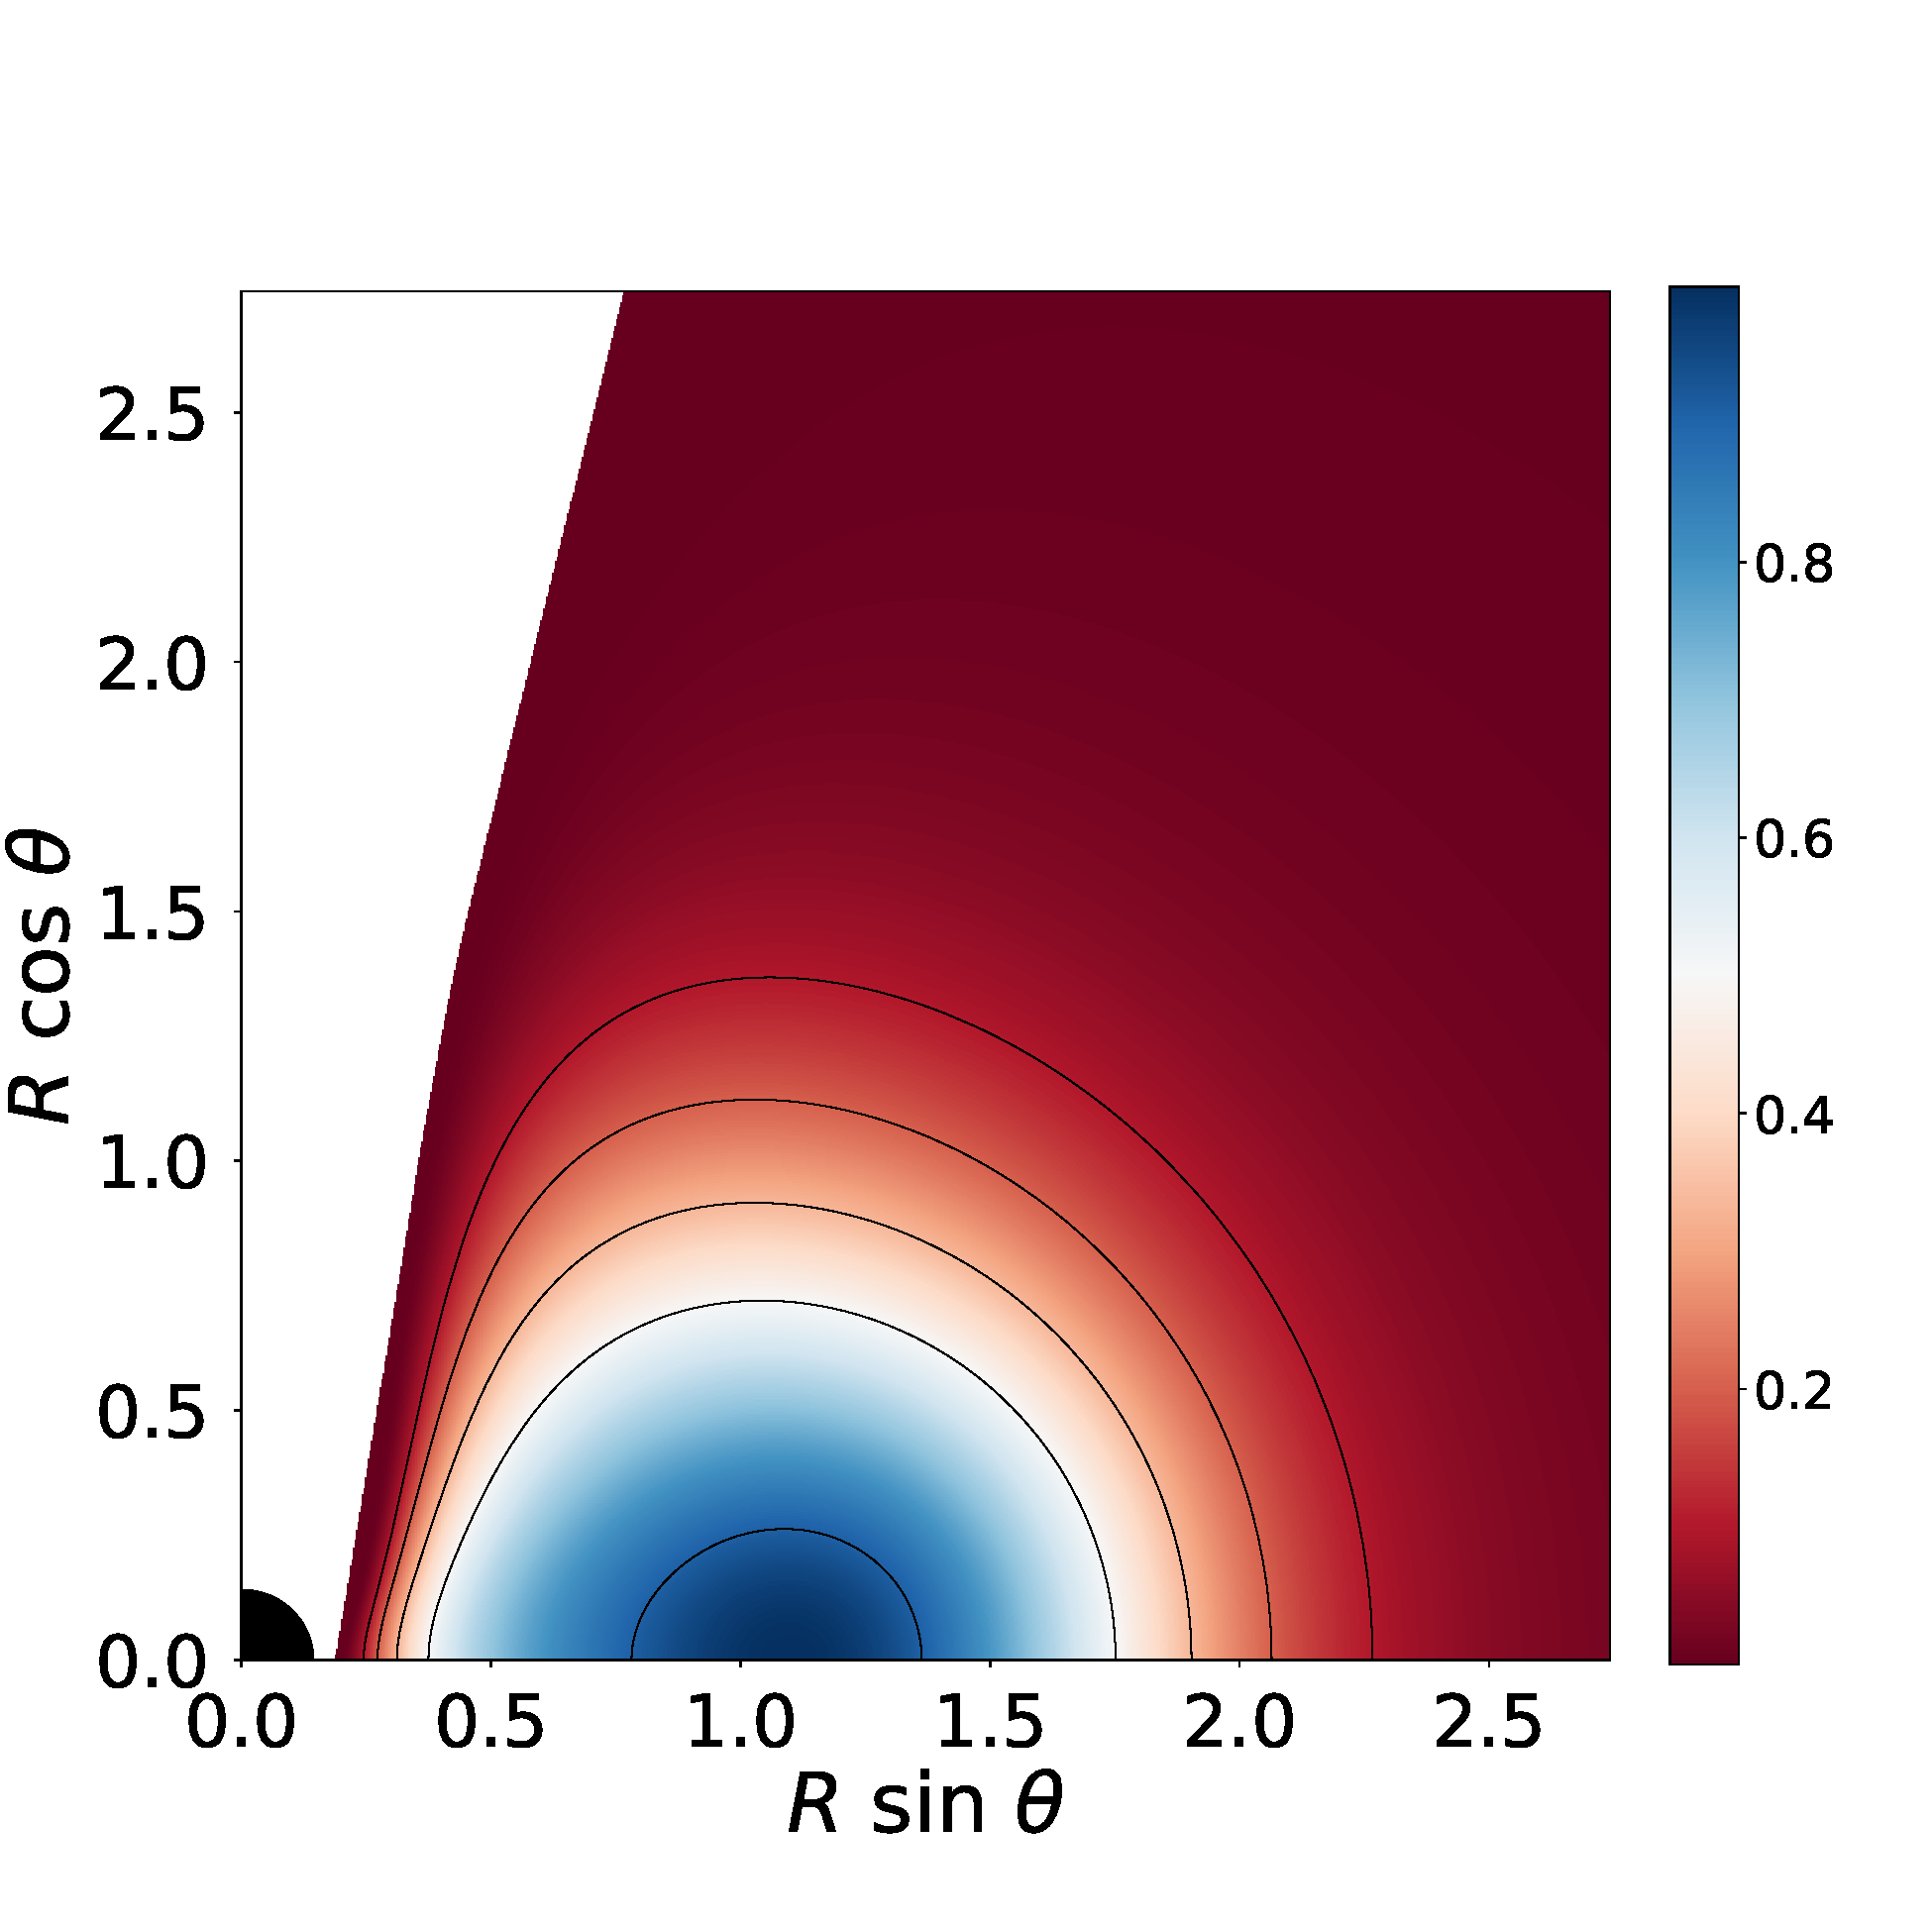
\includegraphics[scale=0.14]{figures/fig4_VII_10.pdf}
\hspace{-0.3cm}
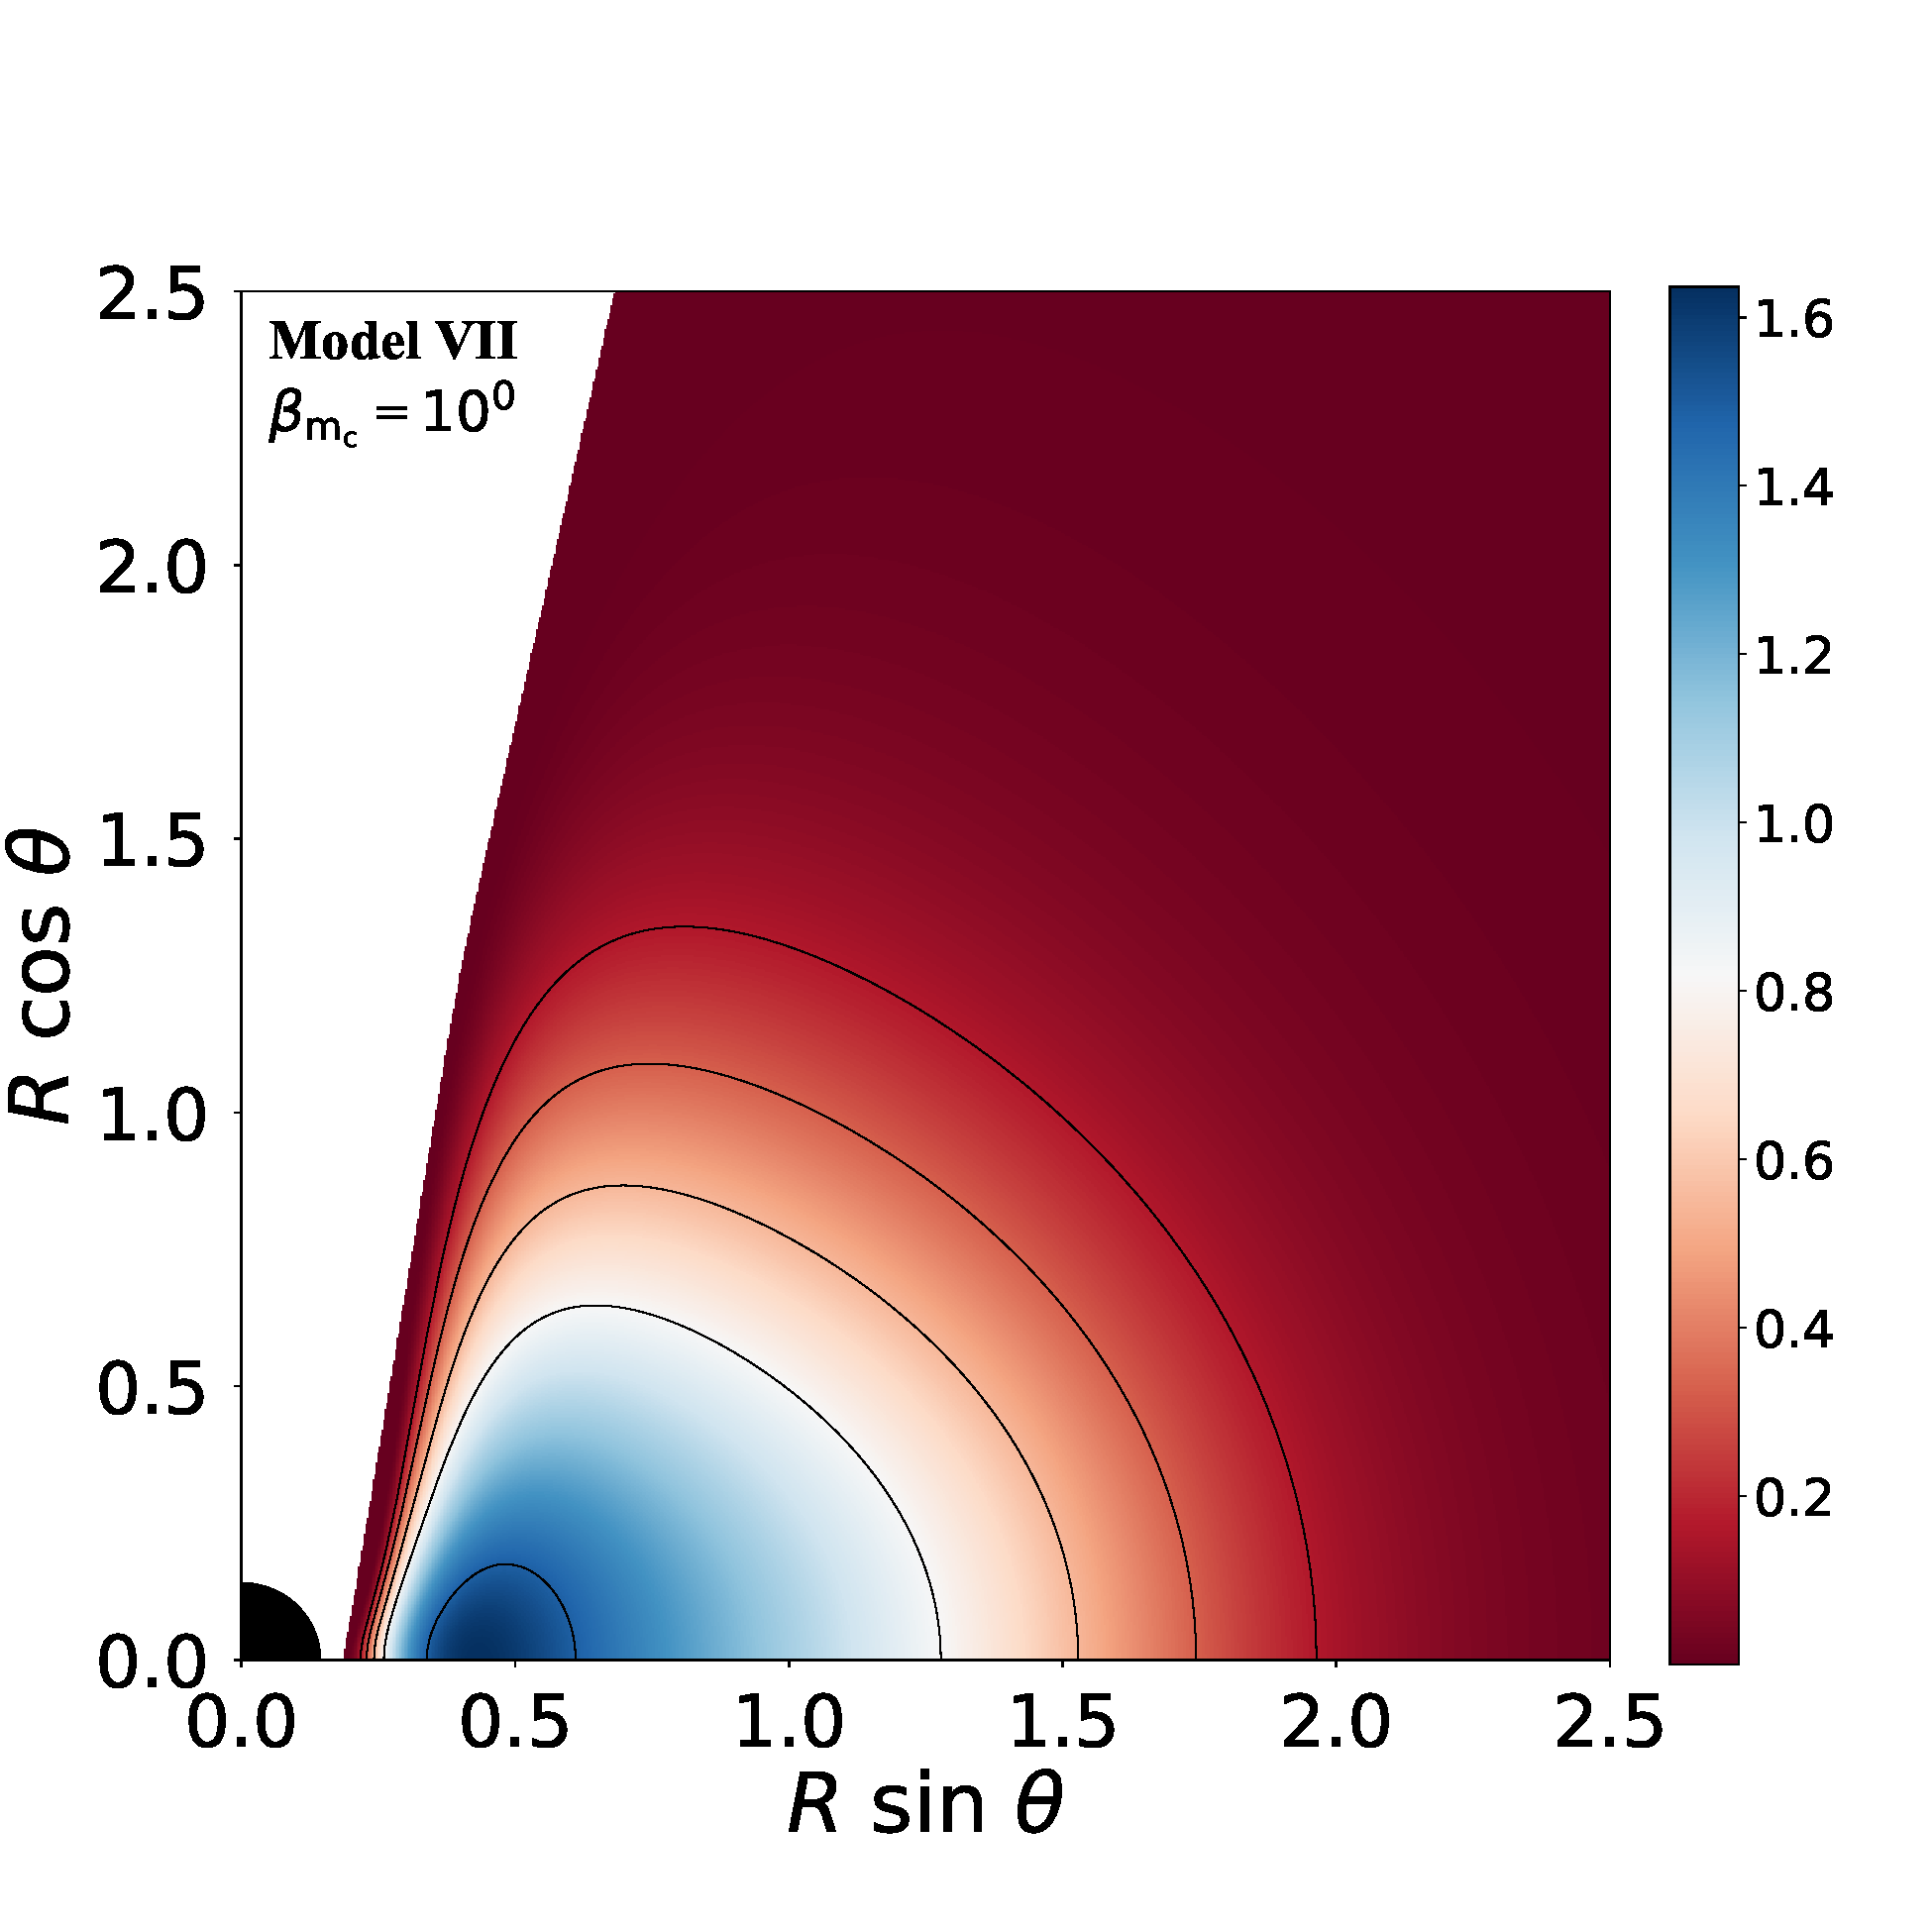
\includegraphics[scale=0.14]{figures/fig4_VII_1.pdf}
\hspace{-0.2cm}
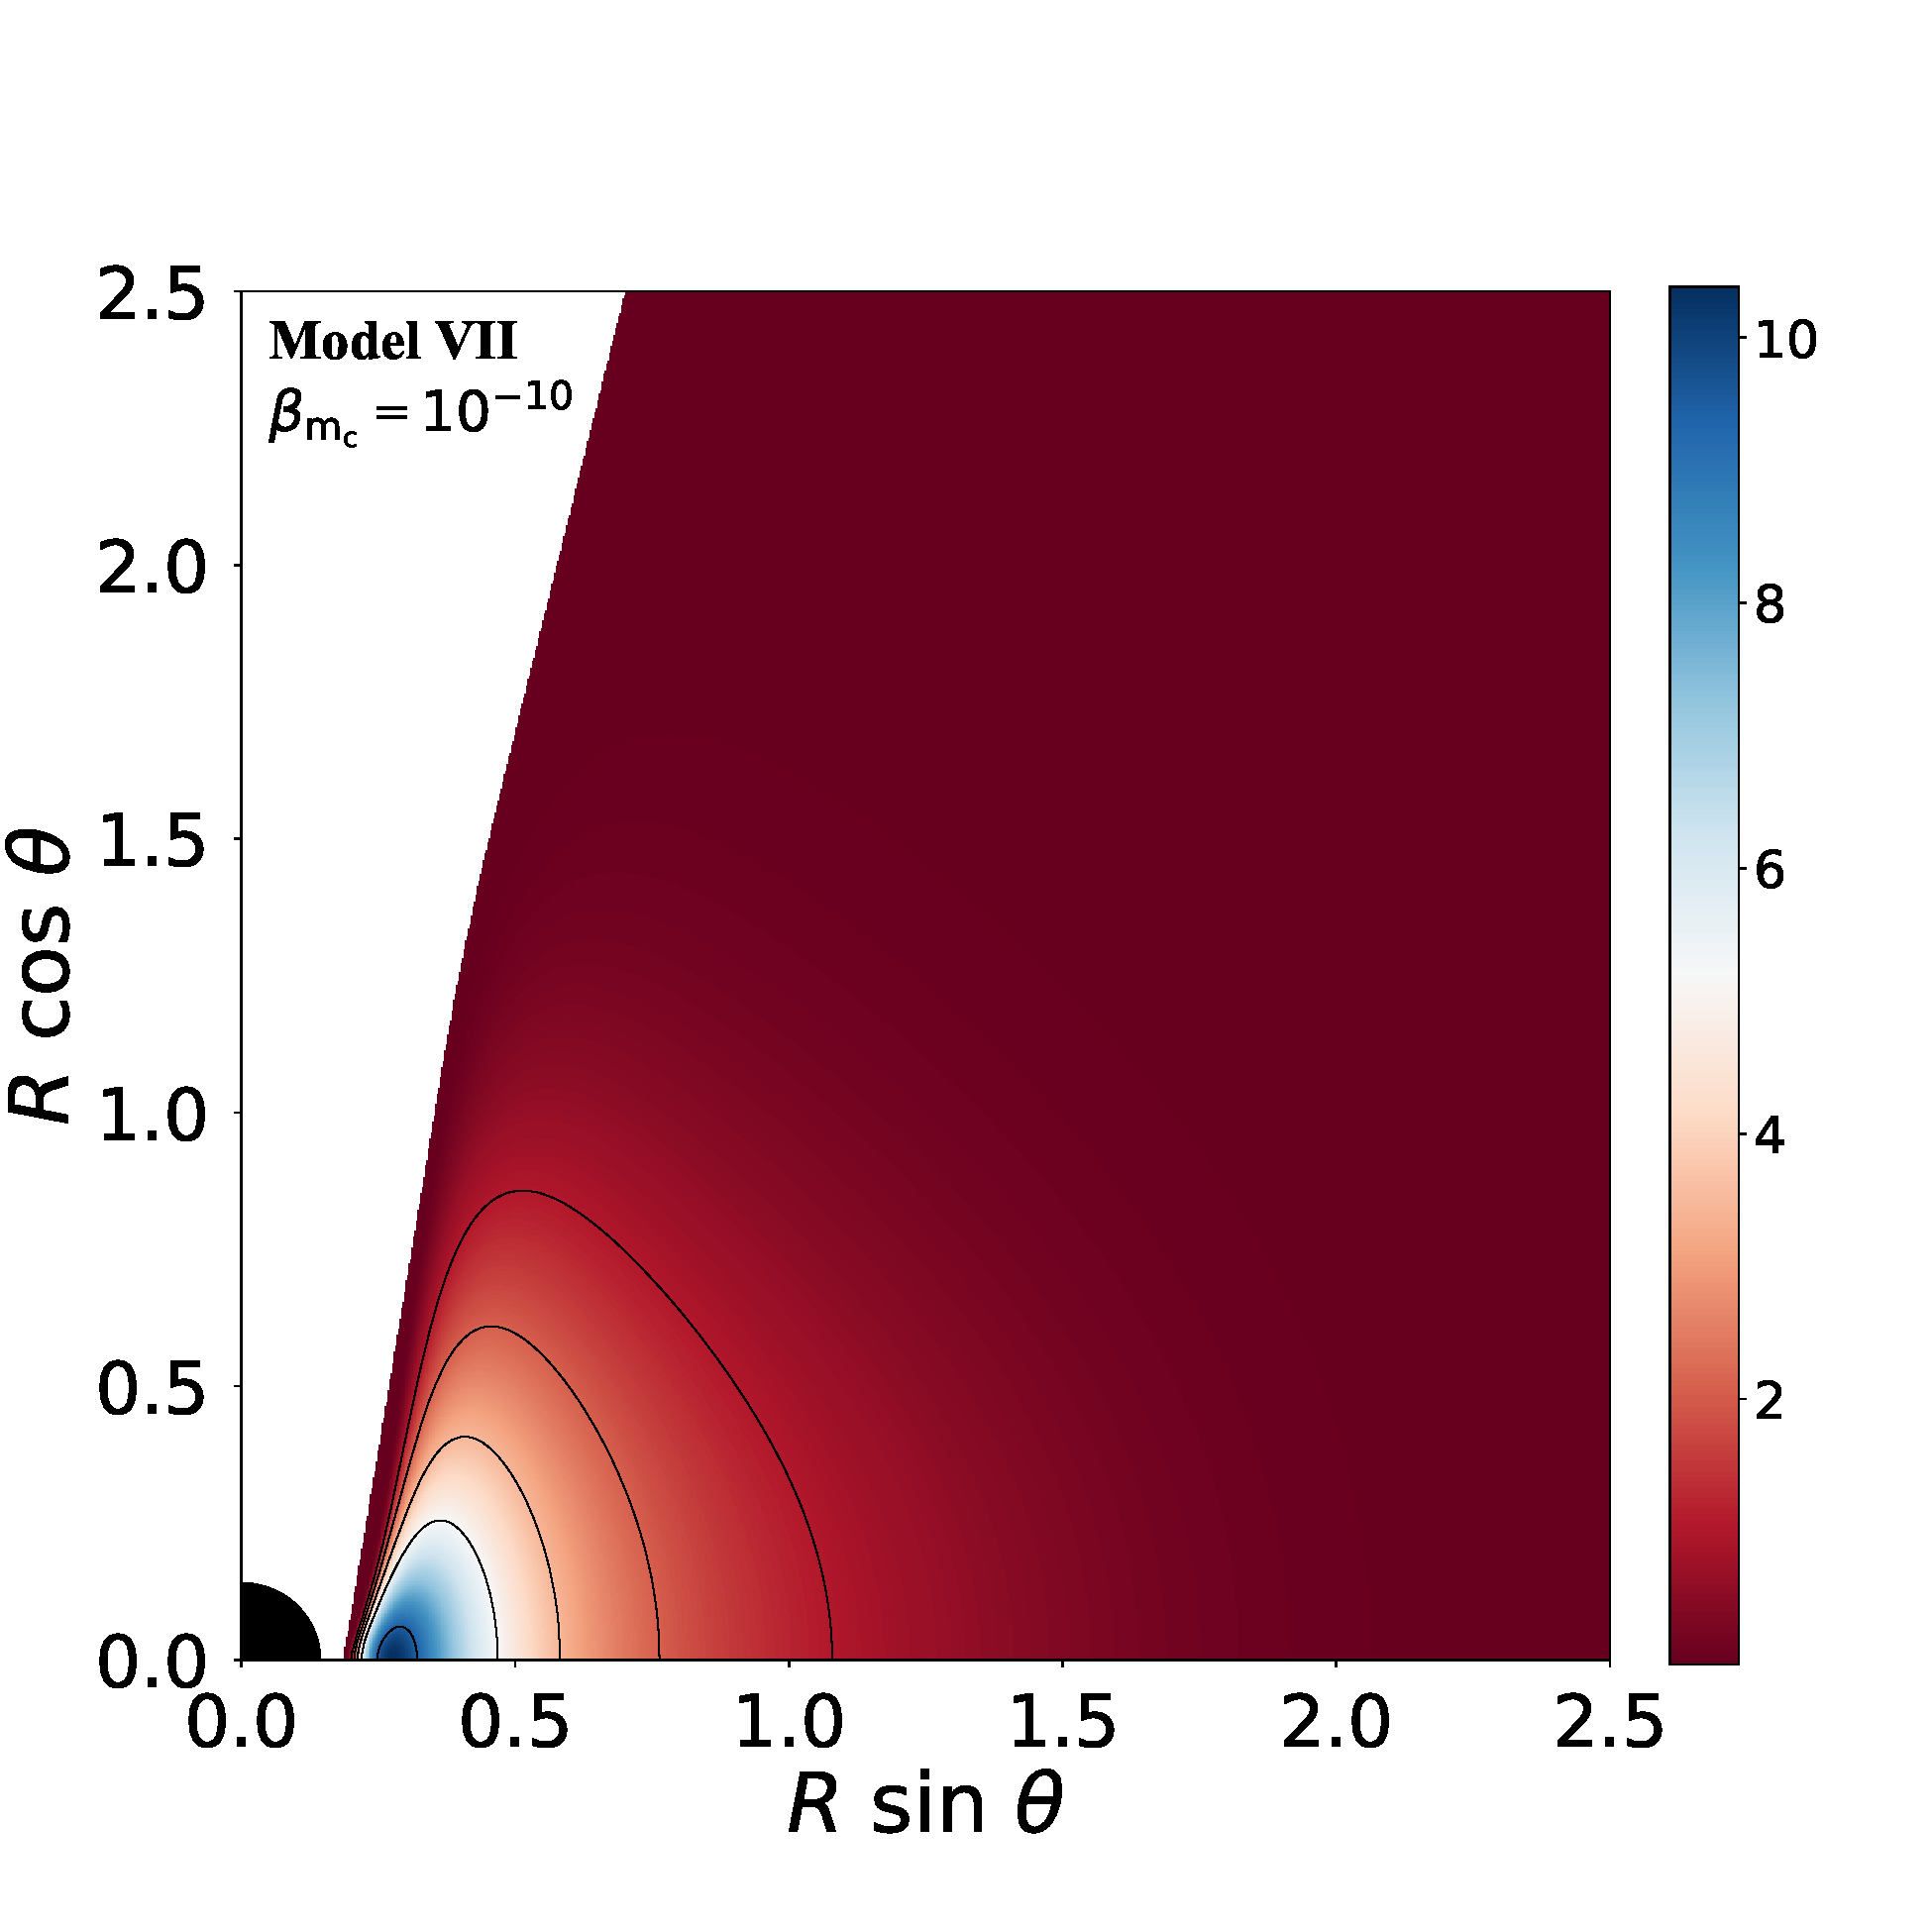
\includegraphics[scale=0.14]{figures/fig4_VII__10.pdf}
\hspace{-0.2cm}
\caption{Rest-mass density distribution using perimeteral coordinates. From top to bottom the rows correspond to the different models for the KBHsSH (V, VI, VII). From left to right the columns correspond to different values of the magnetization parameter, namely non-magnetized ($\beta_{\mathrm{m}_{\mathrm{c}}} = 10^{10}$), mildly magnetized ($\beta_{\mathrm{m}_{\mathrm{c}}} = 1$) and strongly magnetized ($\beta_{\mathrm{m}_{\mathrm{c}}} = 10^{-10}$)}
\label{models_peri_II}
\end{figure*}

\begin{figure*}
\centering
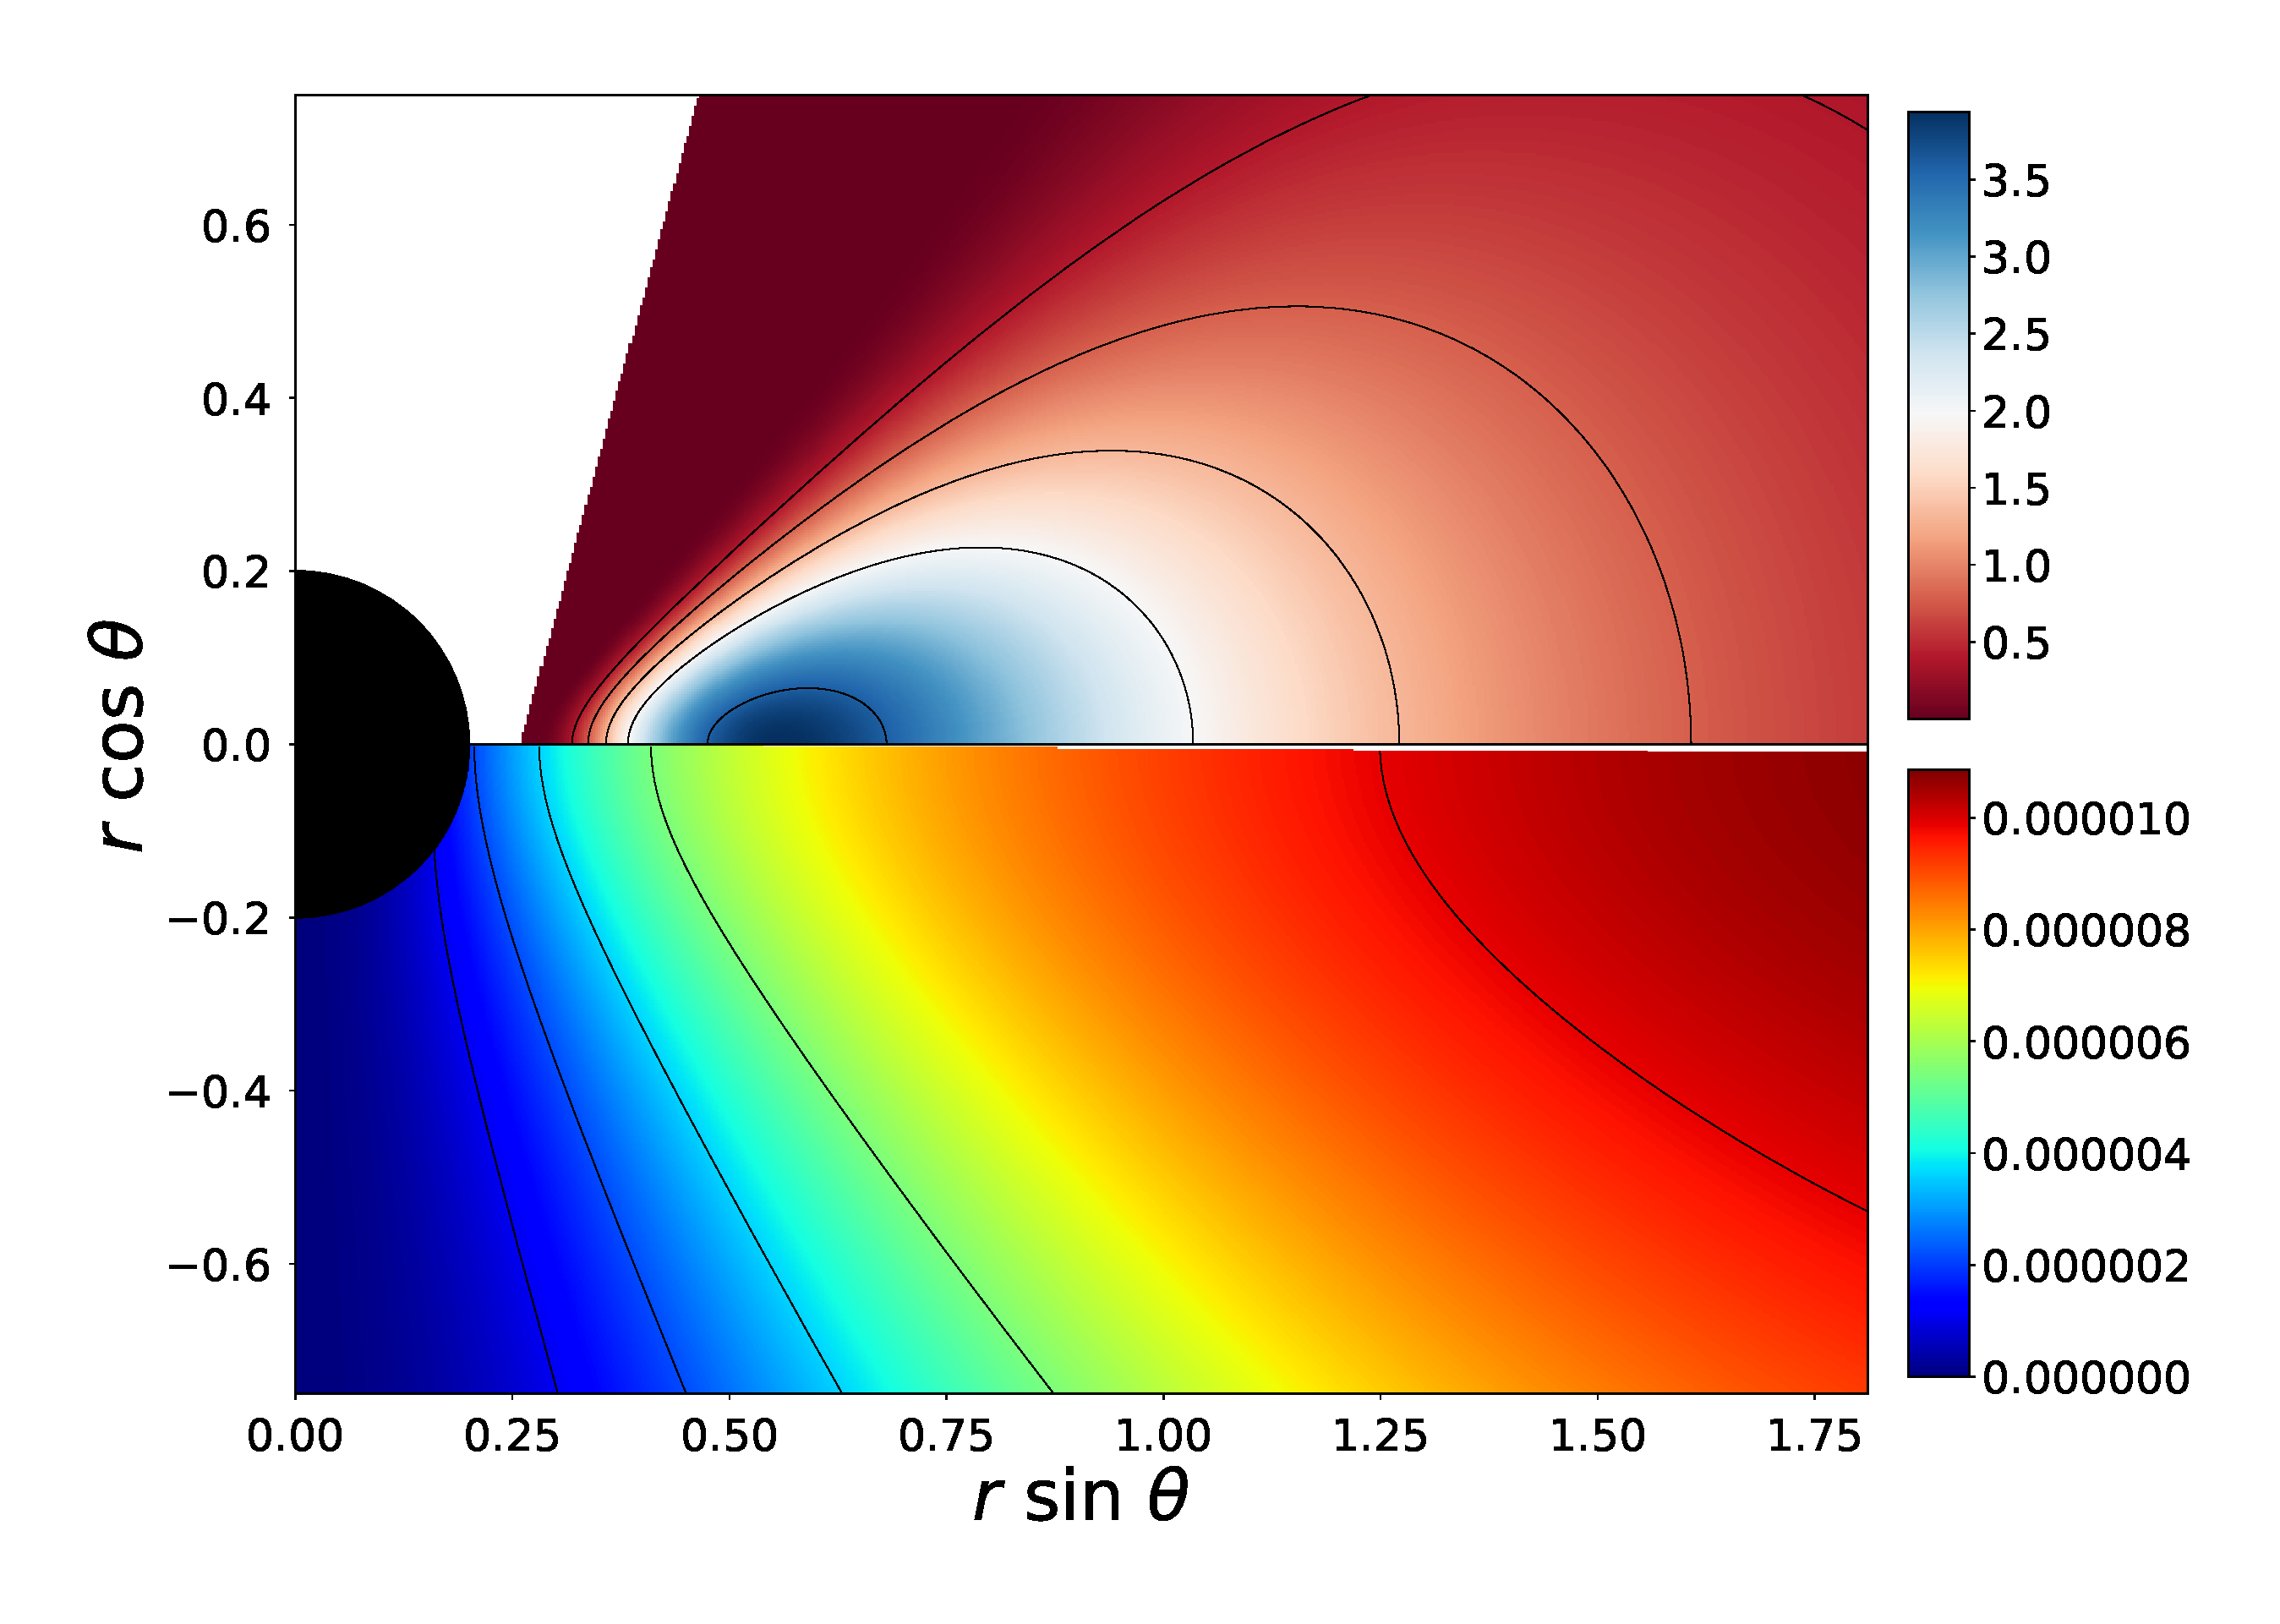
\includegraphics[scale=0.12]{figures/fig5_I_10.pdf}
\hspace{-0.3cm}
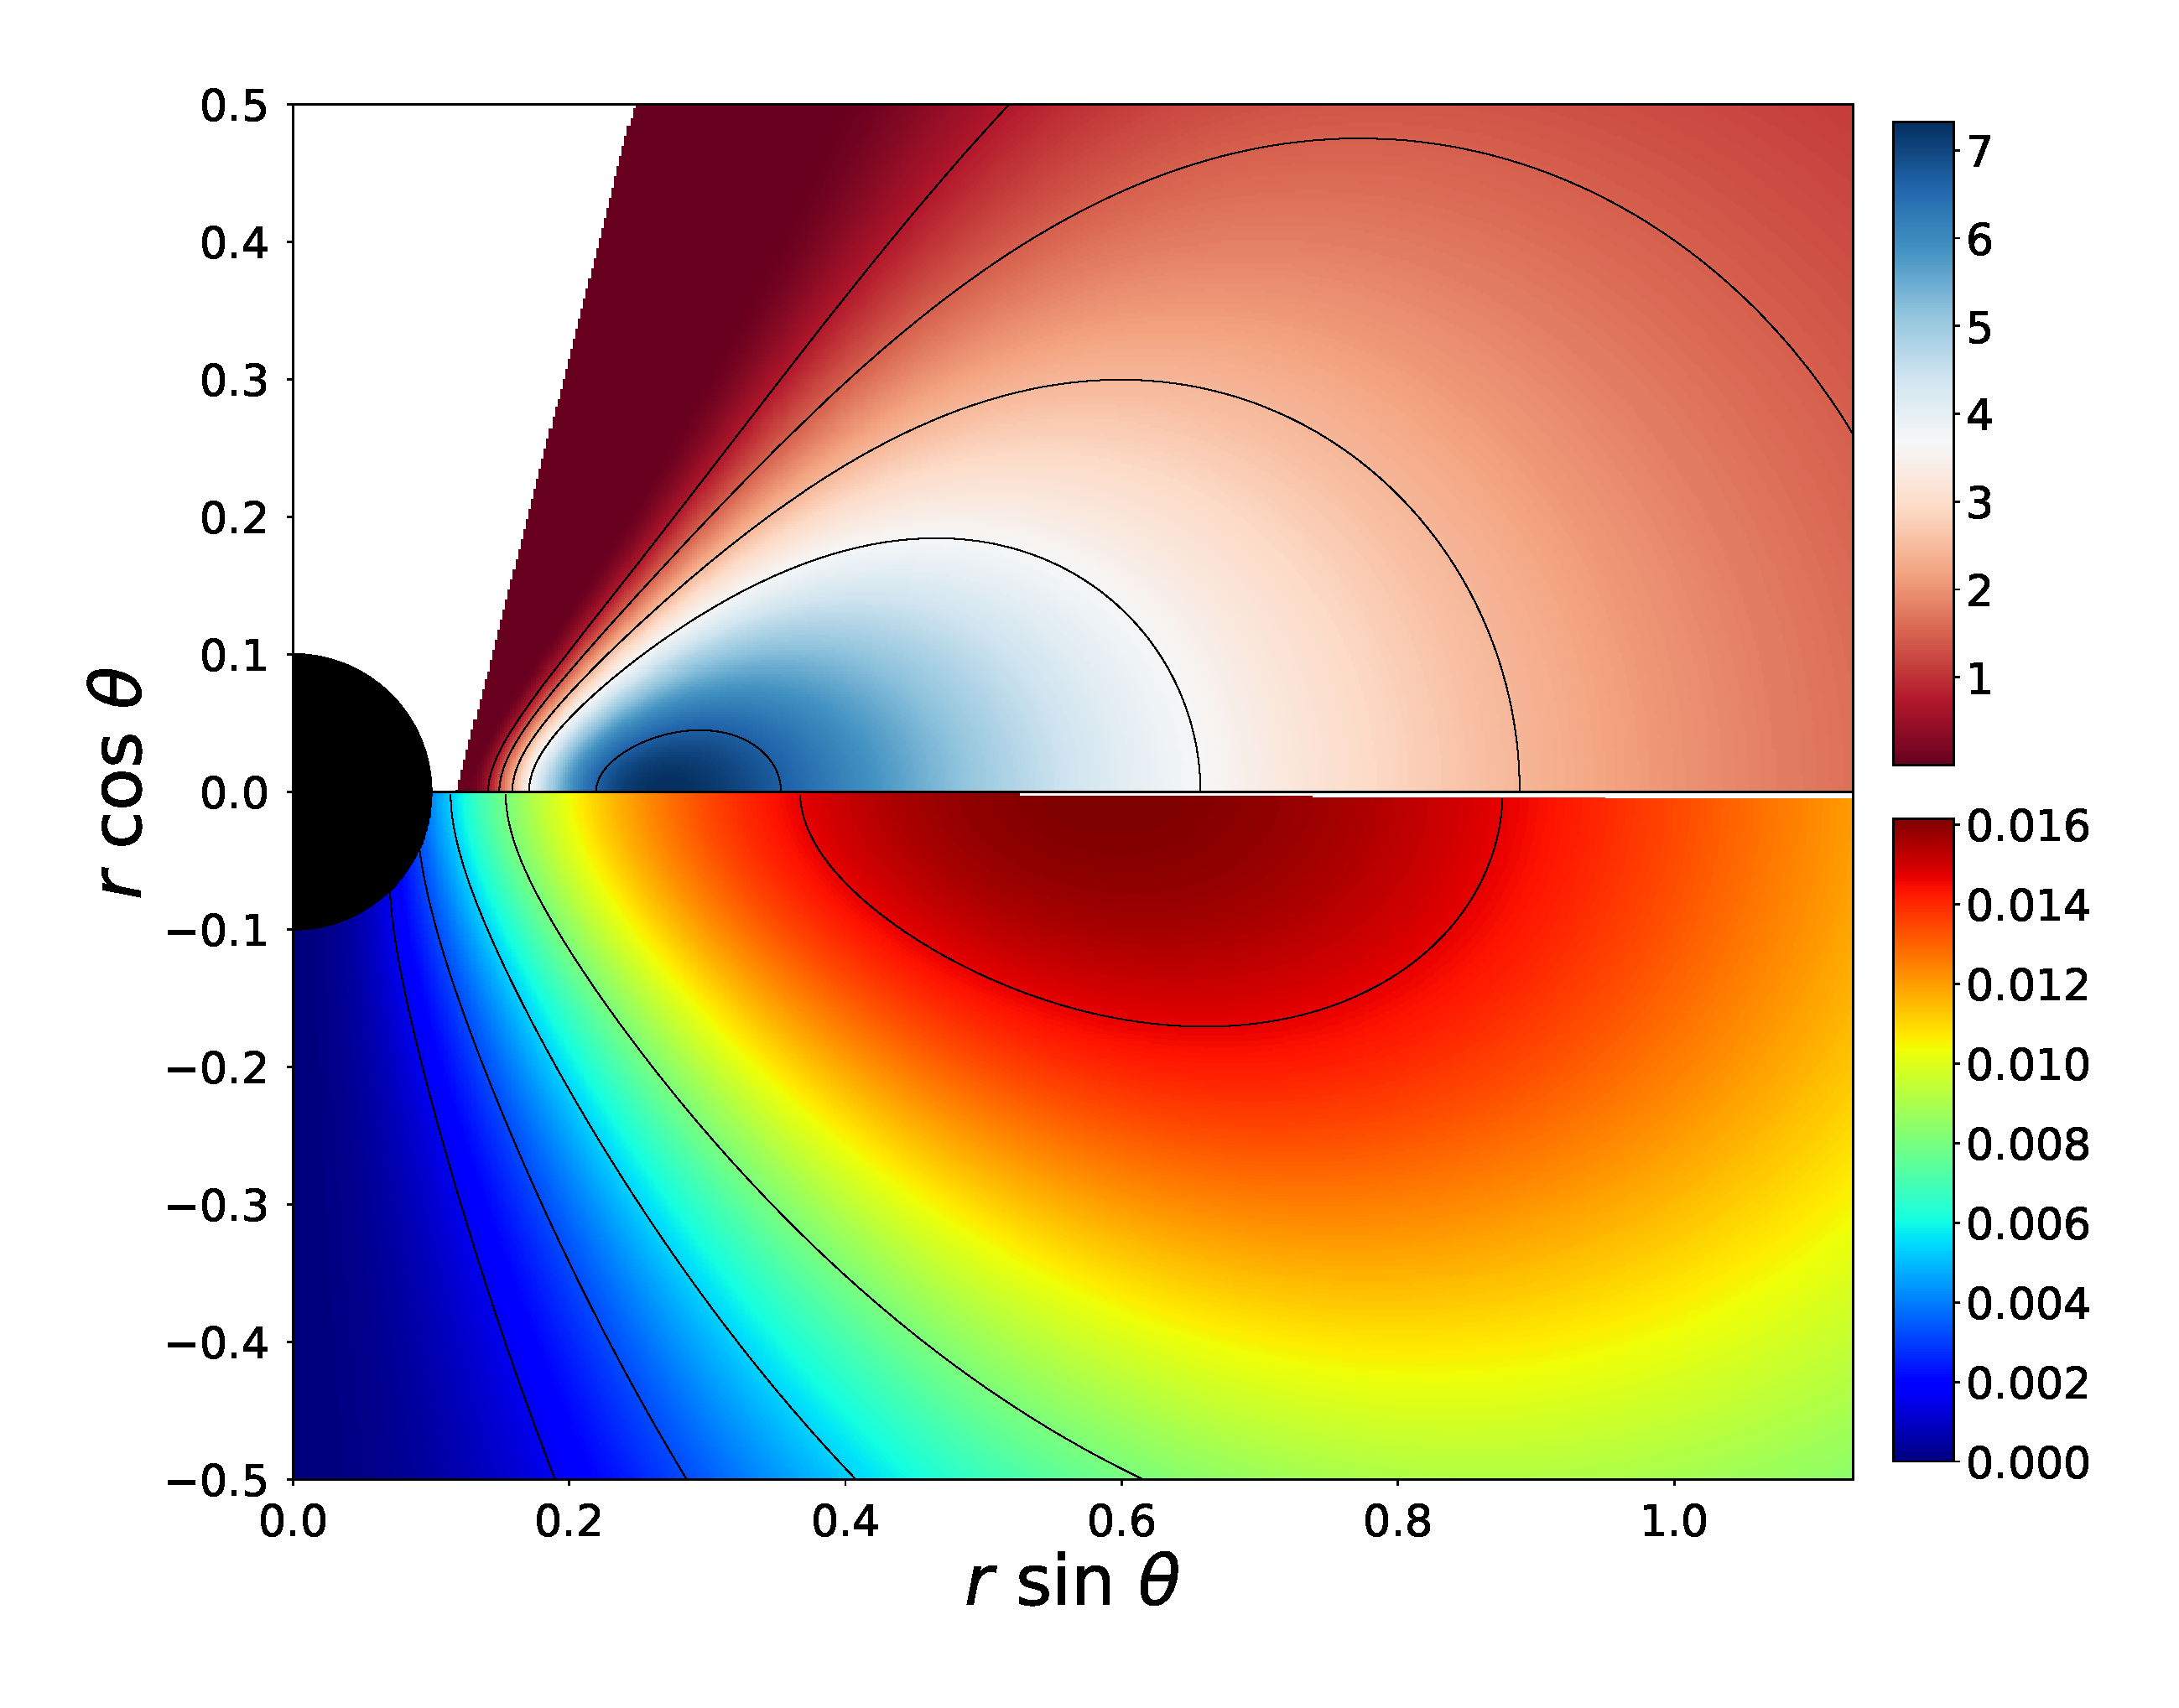
\includegraphics[scale=0.12]{figures/fig5_IV_10.pdf}
\hspace{-0.3cm}
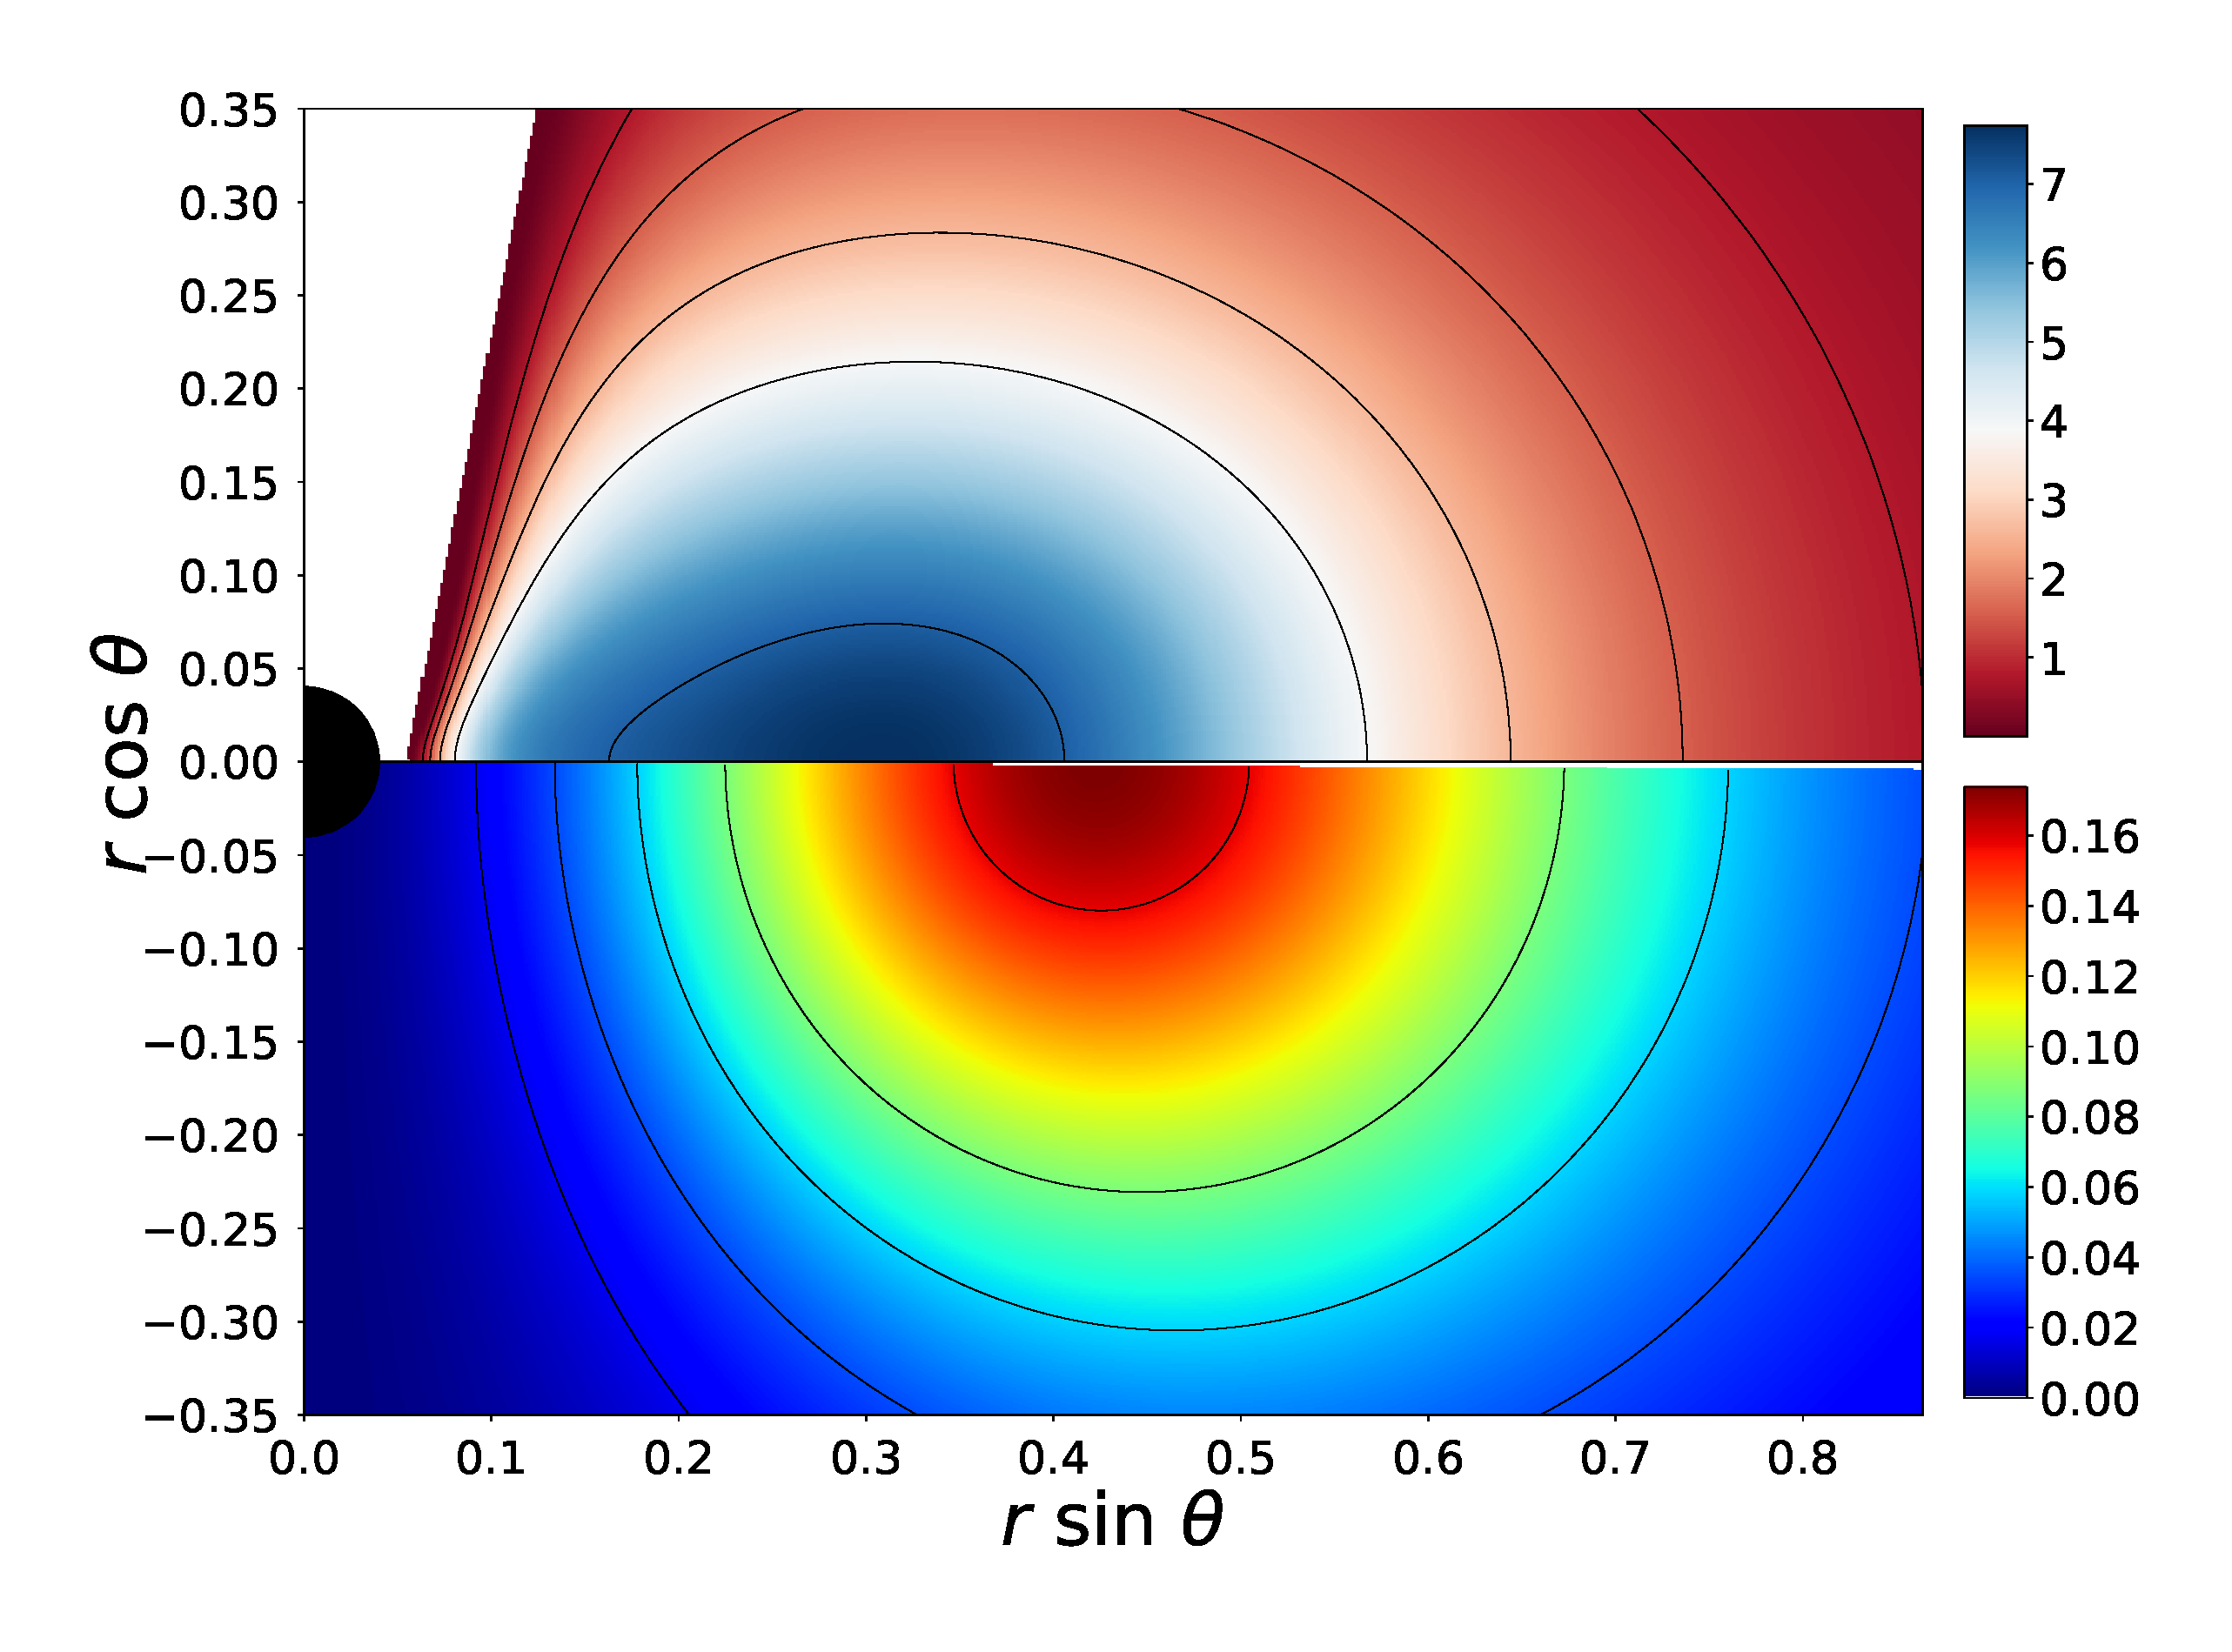
\includegraphics[scale=0.12]{figures/fig5_VII_10.pdf}
\hspace{-0.2cm}
\\
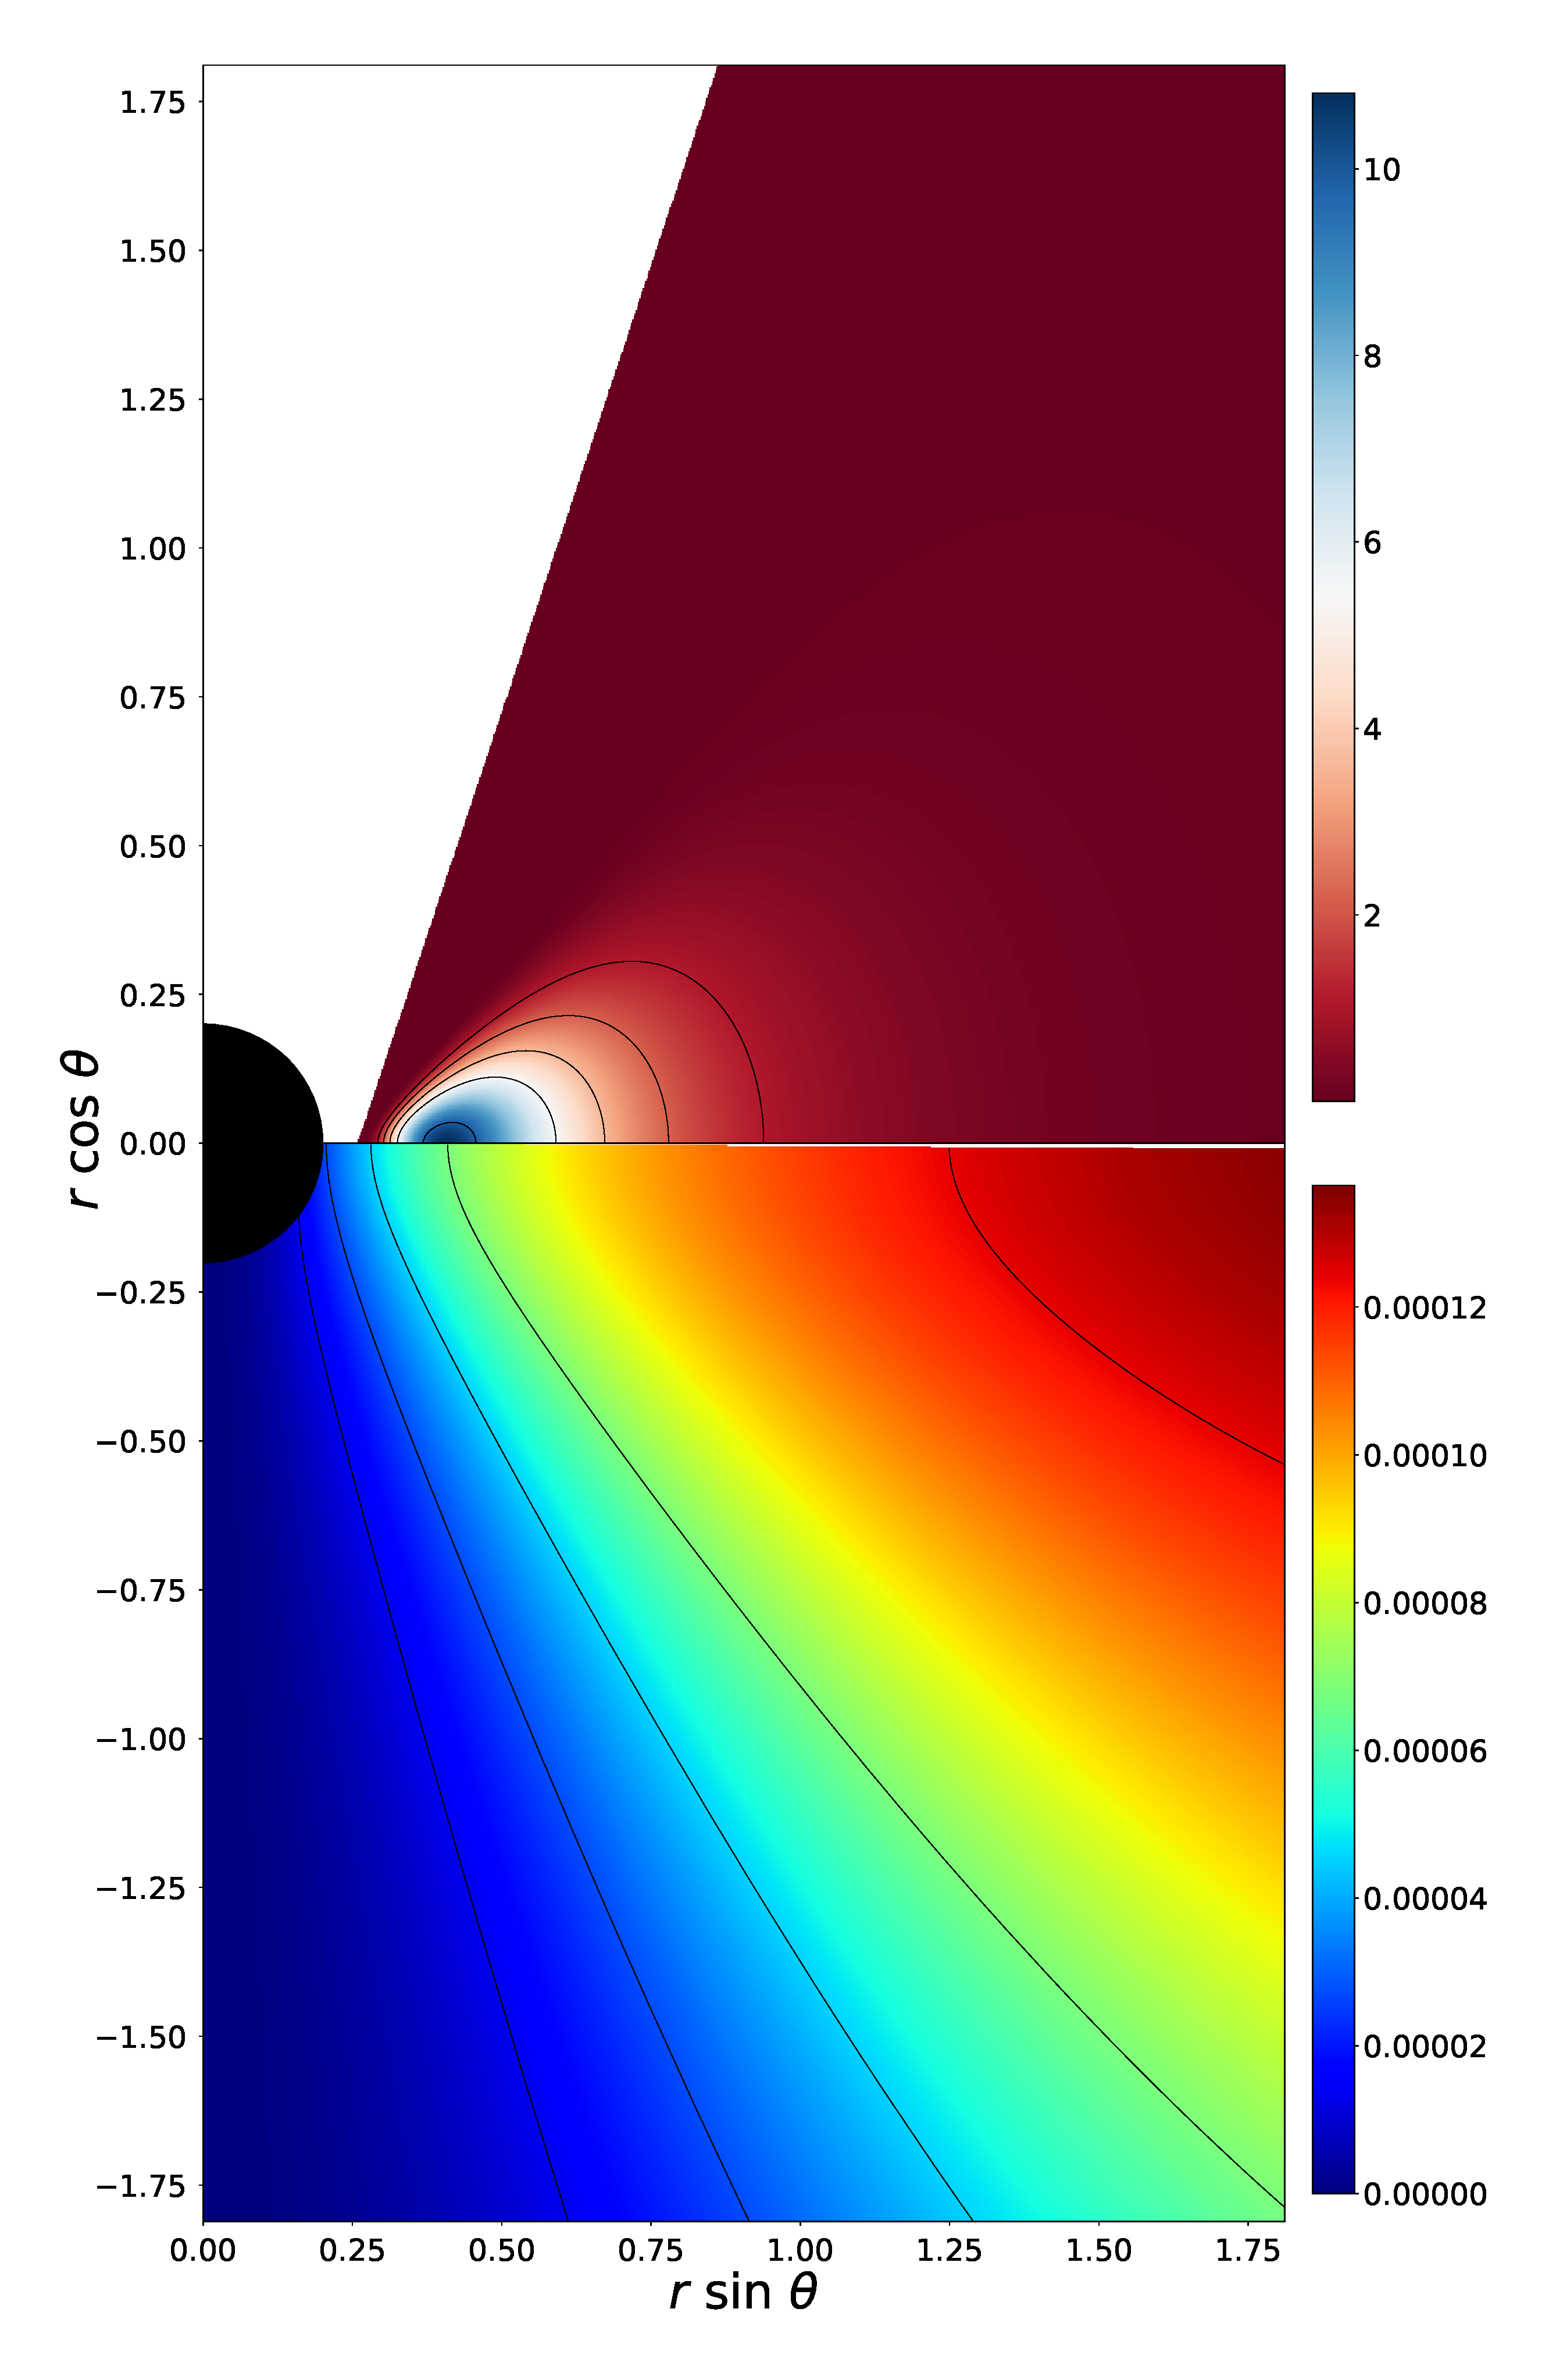
\includegraphics[scale=0.12]{figures/fig5_I__10.pdf}
\hspace{-0.3cm}
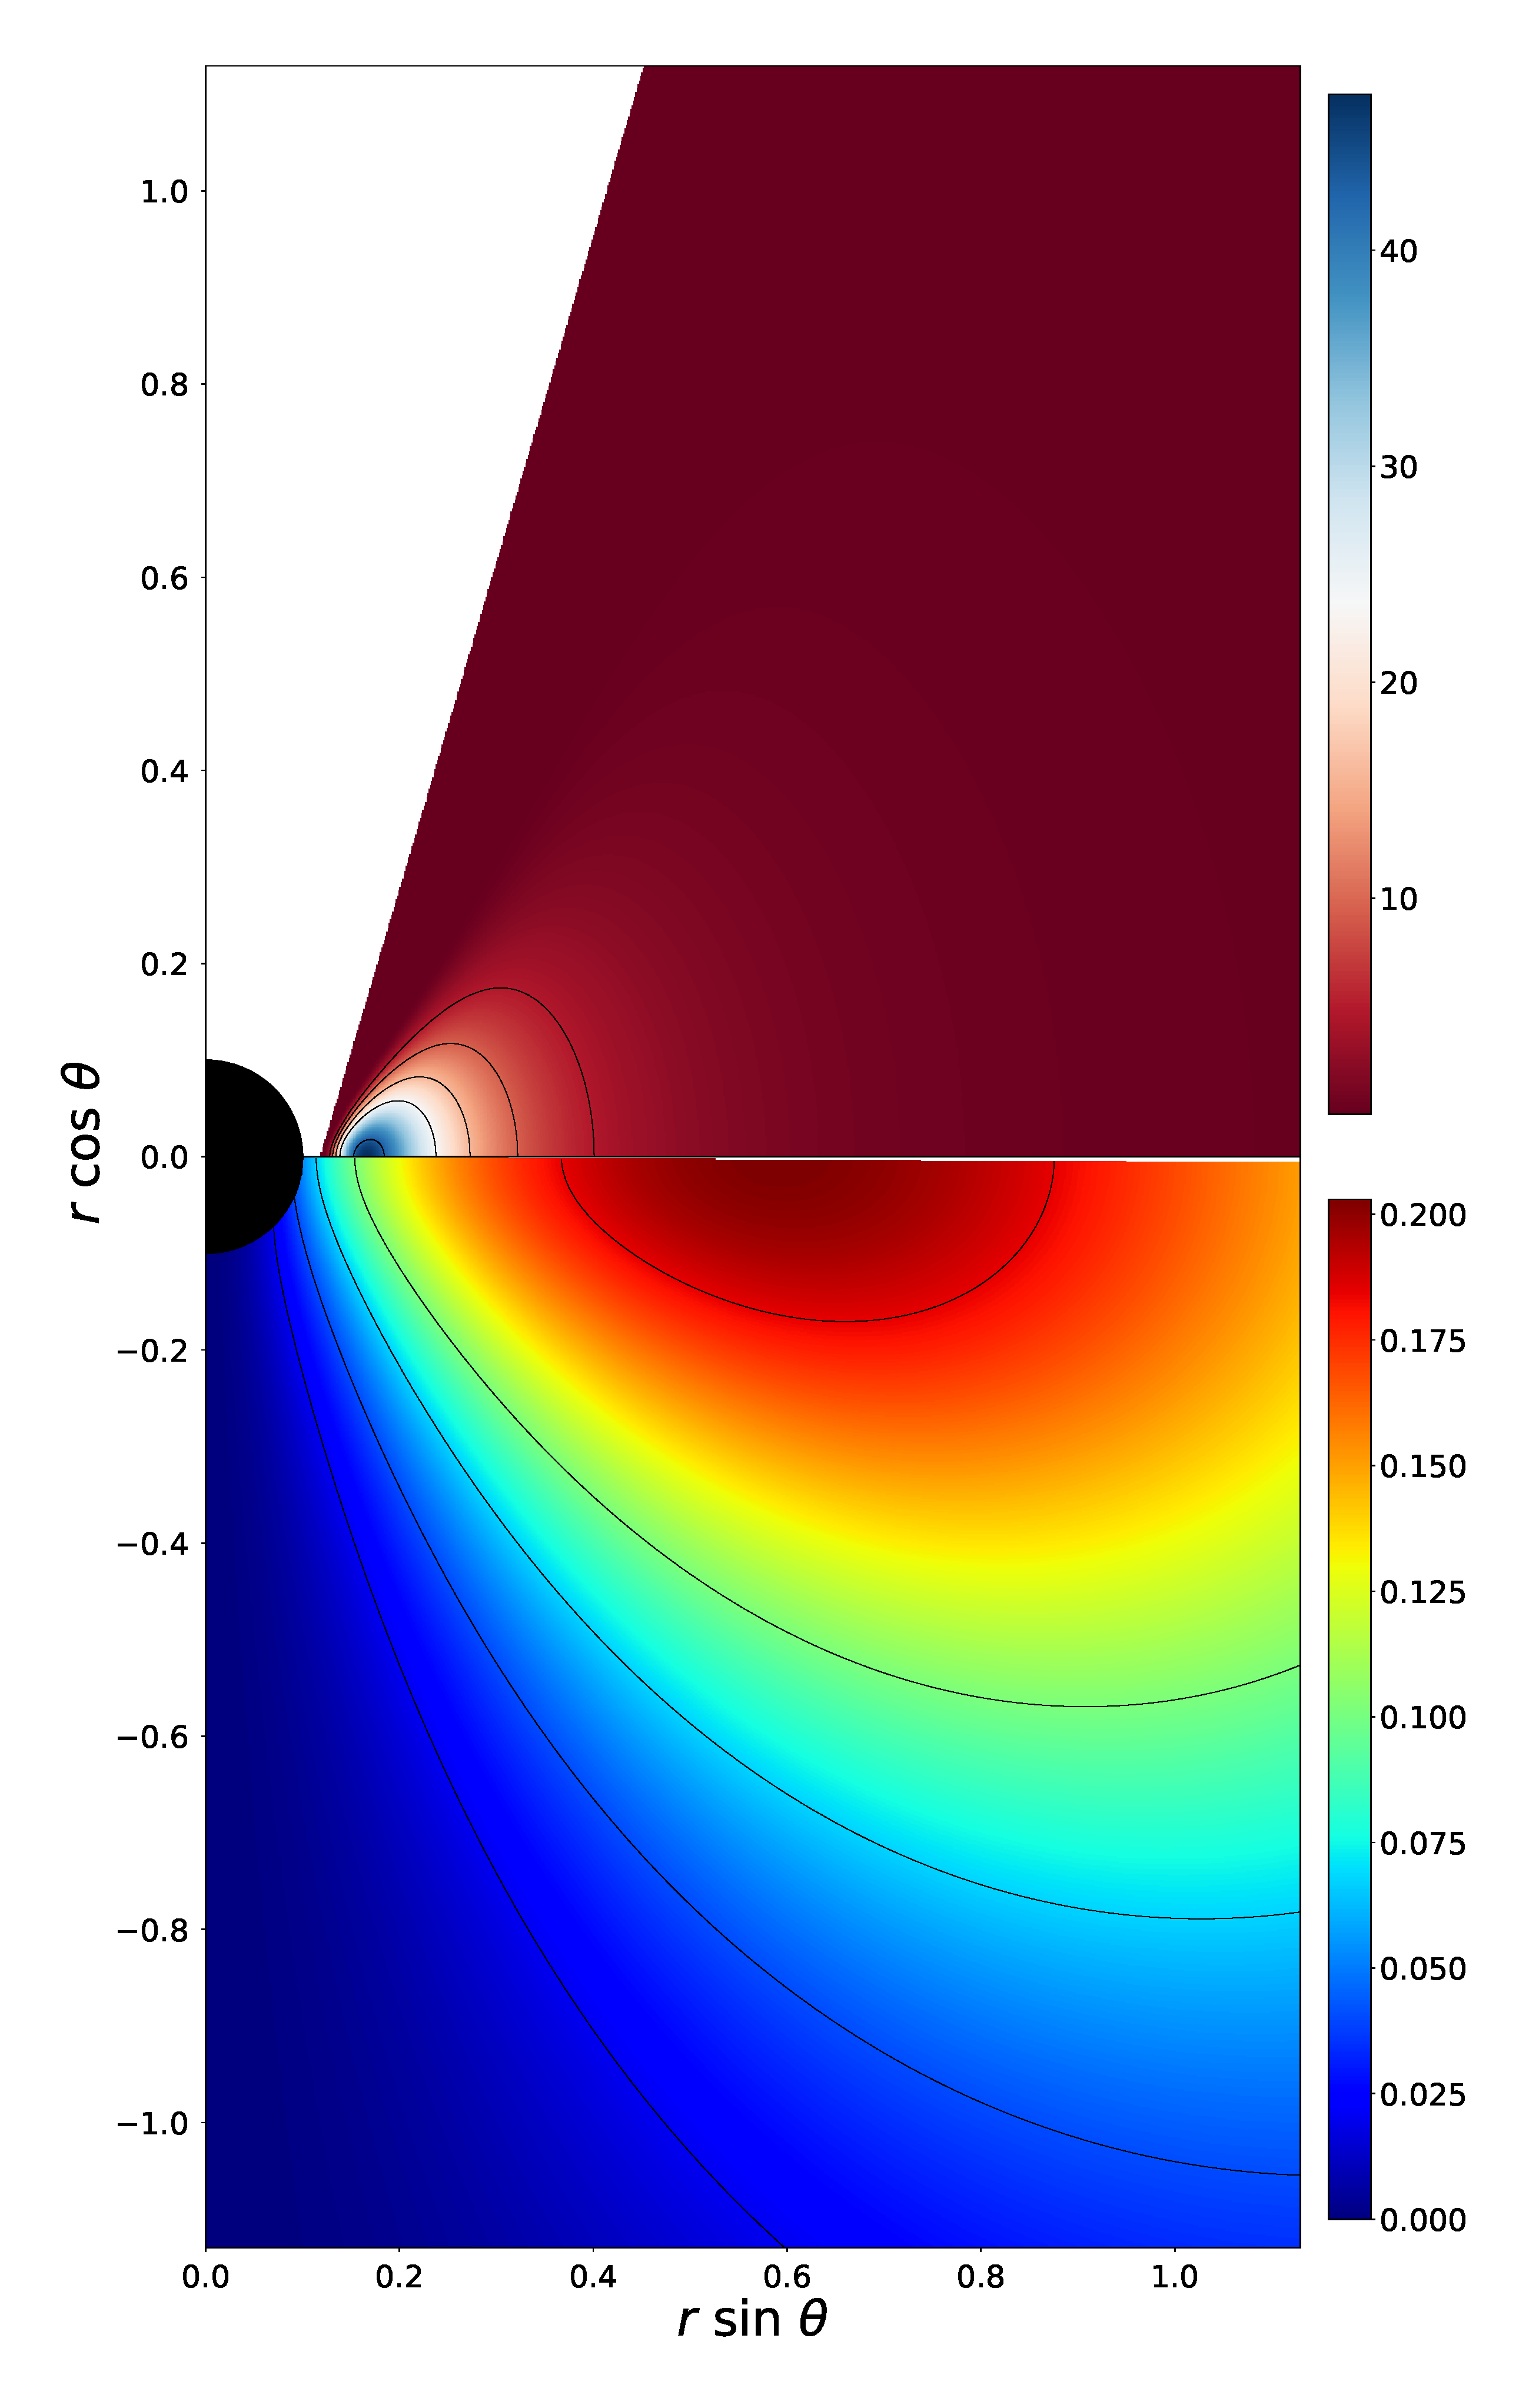
\includegraphics[scale=0.12]{figures/fig5_IV__10.pdf}
\hspace{-0.3cm}
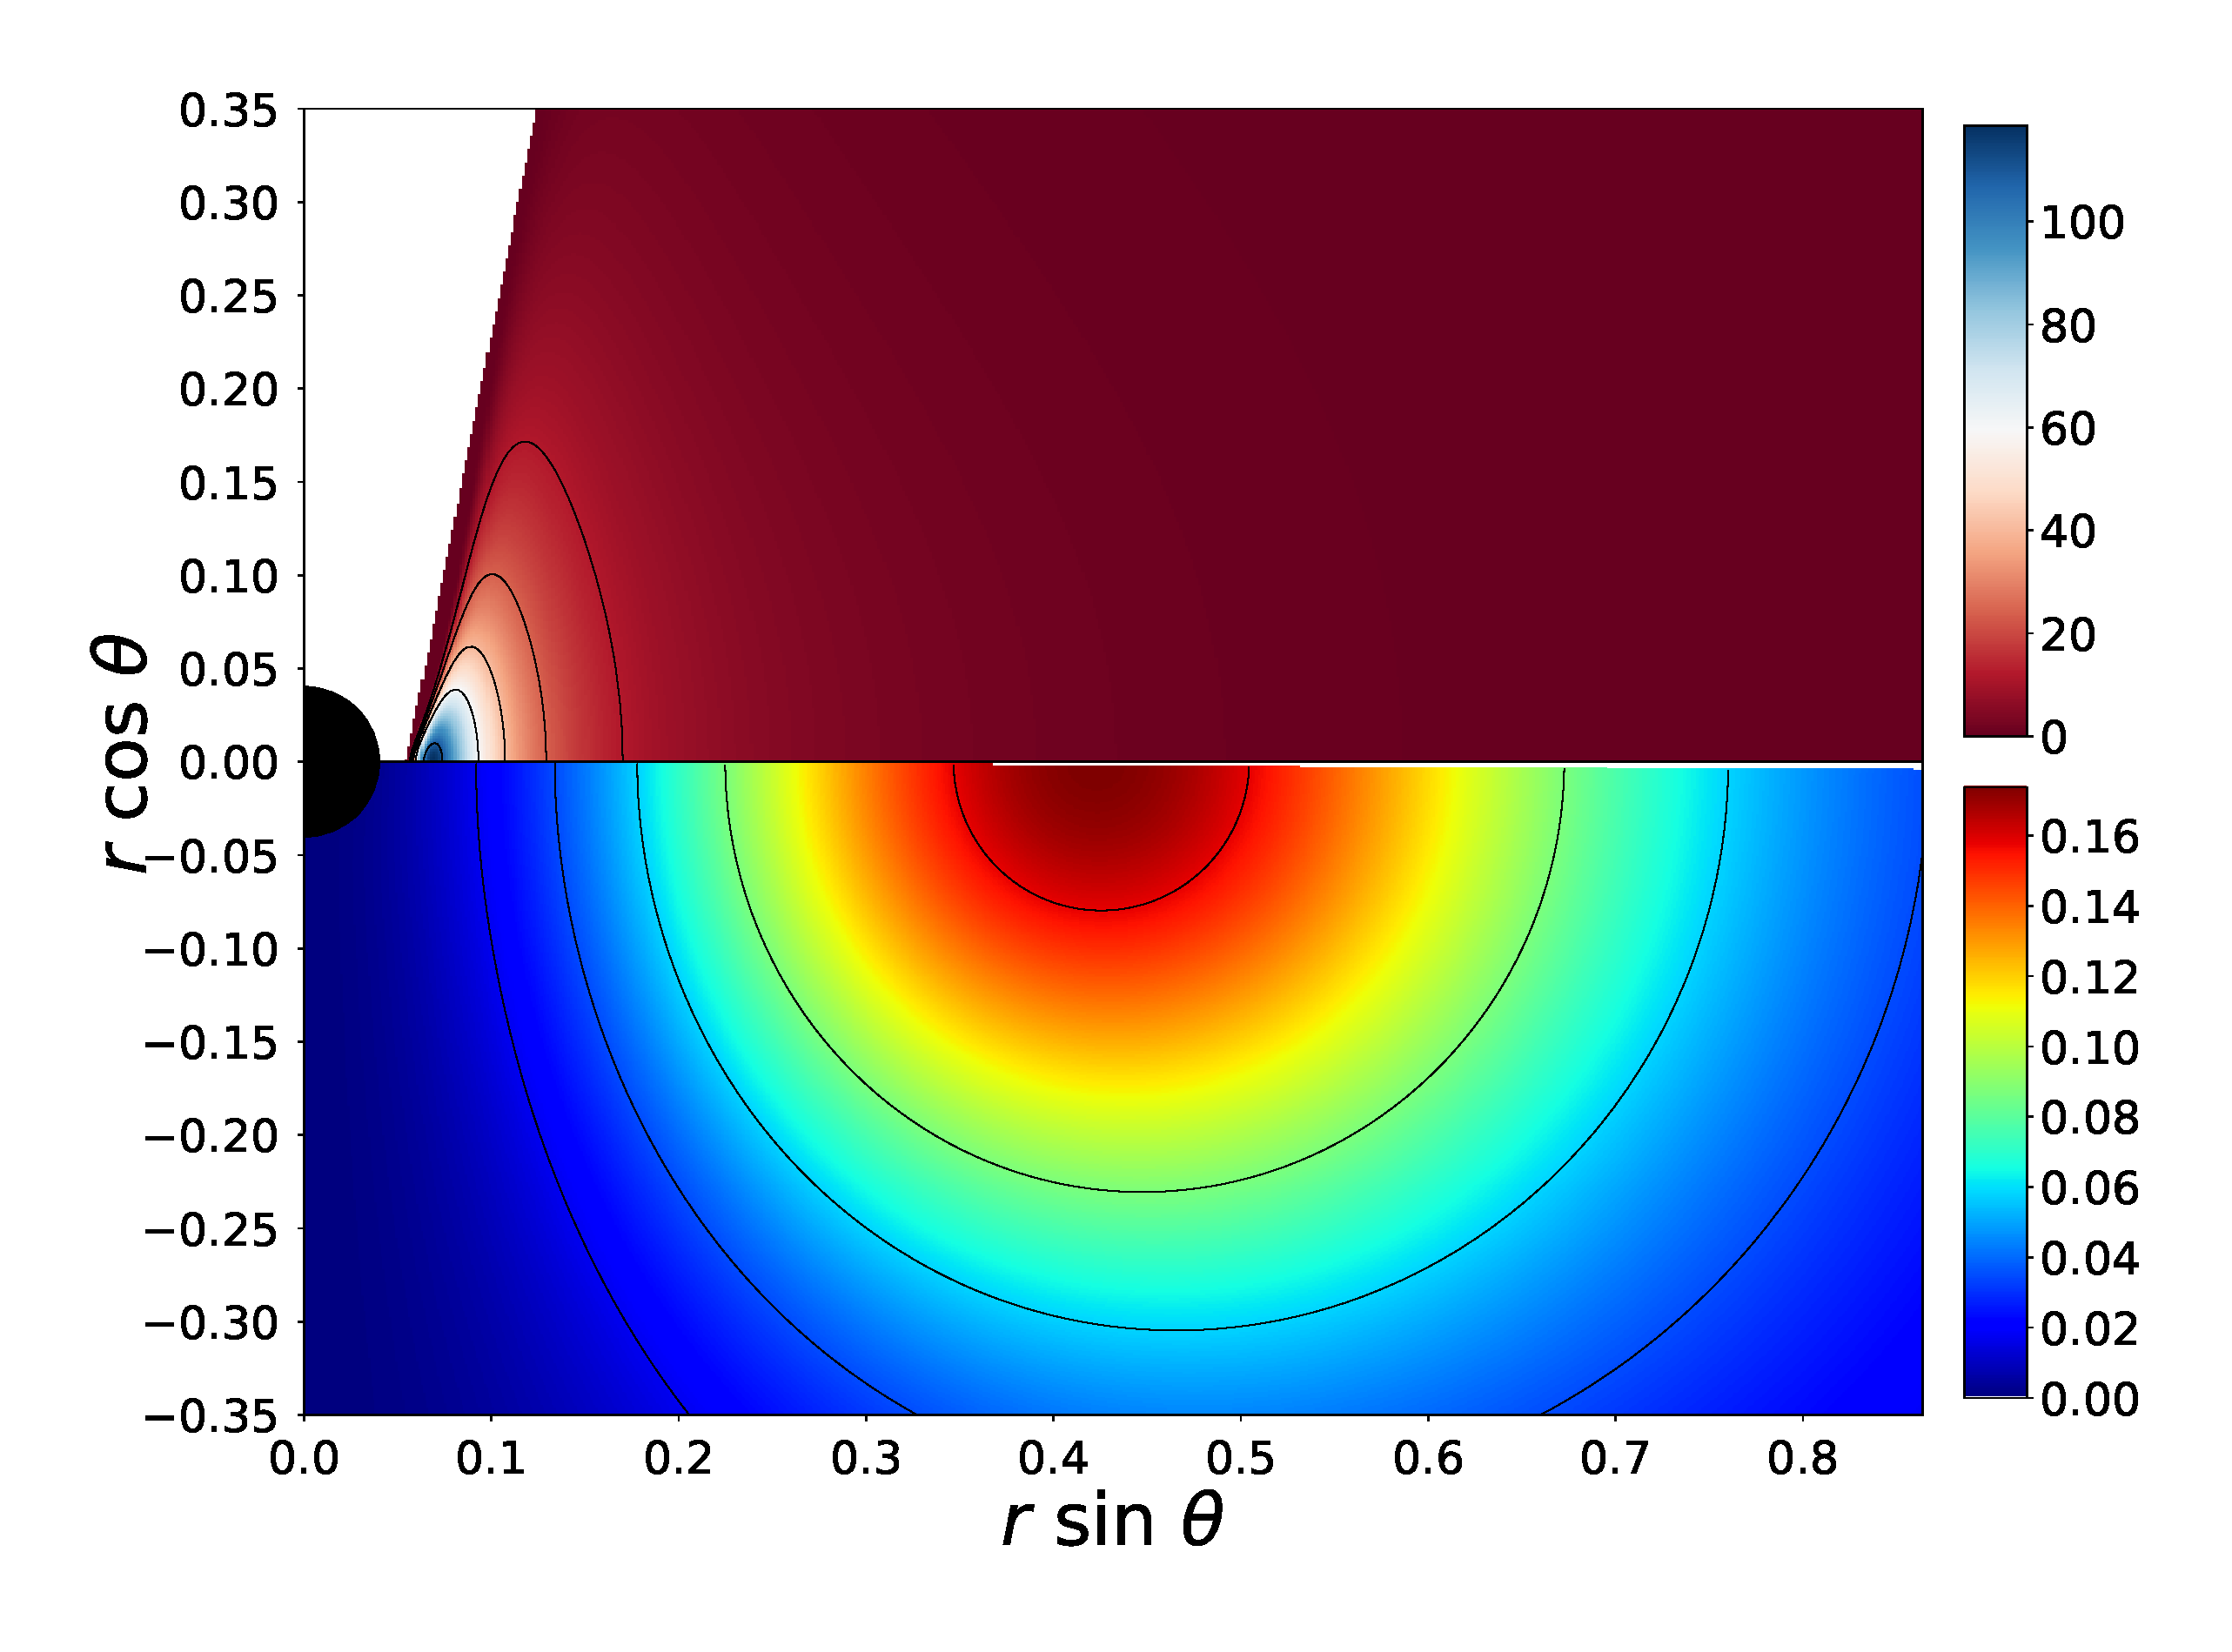
\includegraphics[scale=0.12]{figures/fig5_VII__10.pdf}
\hspace{-0.2cm}
\caption{Gravitational mass density distribution for the torus $\rho_{\mathrm{T}}$ (up) and the scalar field $\rho_{\mathrm{SF}}$ (down). From left to right the columns correspond to different models (I, IV and VII). From top to bottom, the rows correspond to different calues of the magnetization parameter, namely non-magnetized ($\beta_{\mathrm{m}_{\mathrm{c}}} = 10^{10}$) and strongly magnetized ($\beta_{\mathrm{m}_{\mathrm{c}}} = 10^{-10}$)}
\label{comparison_mass_density}
\end{figure*}

\begin{figure*}
\centering
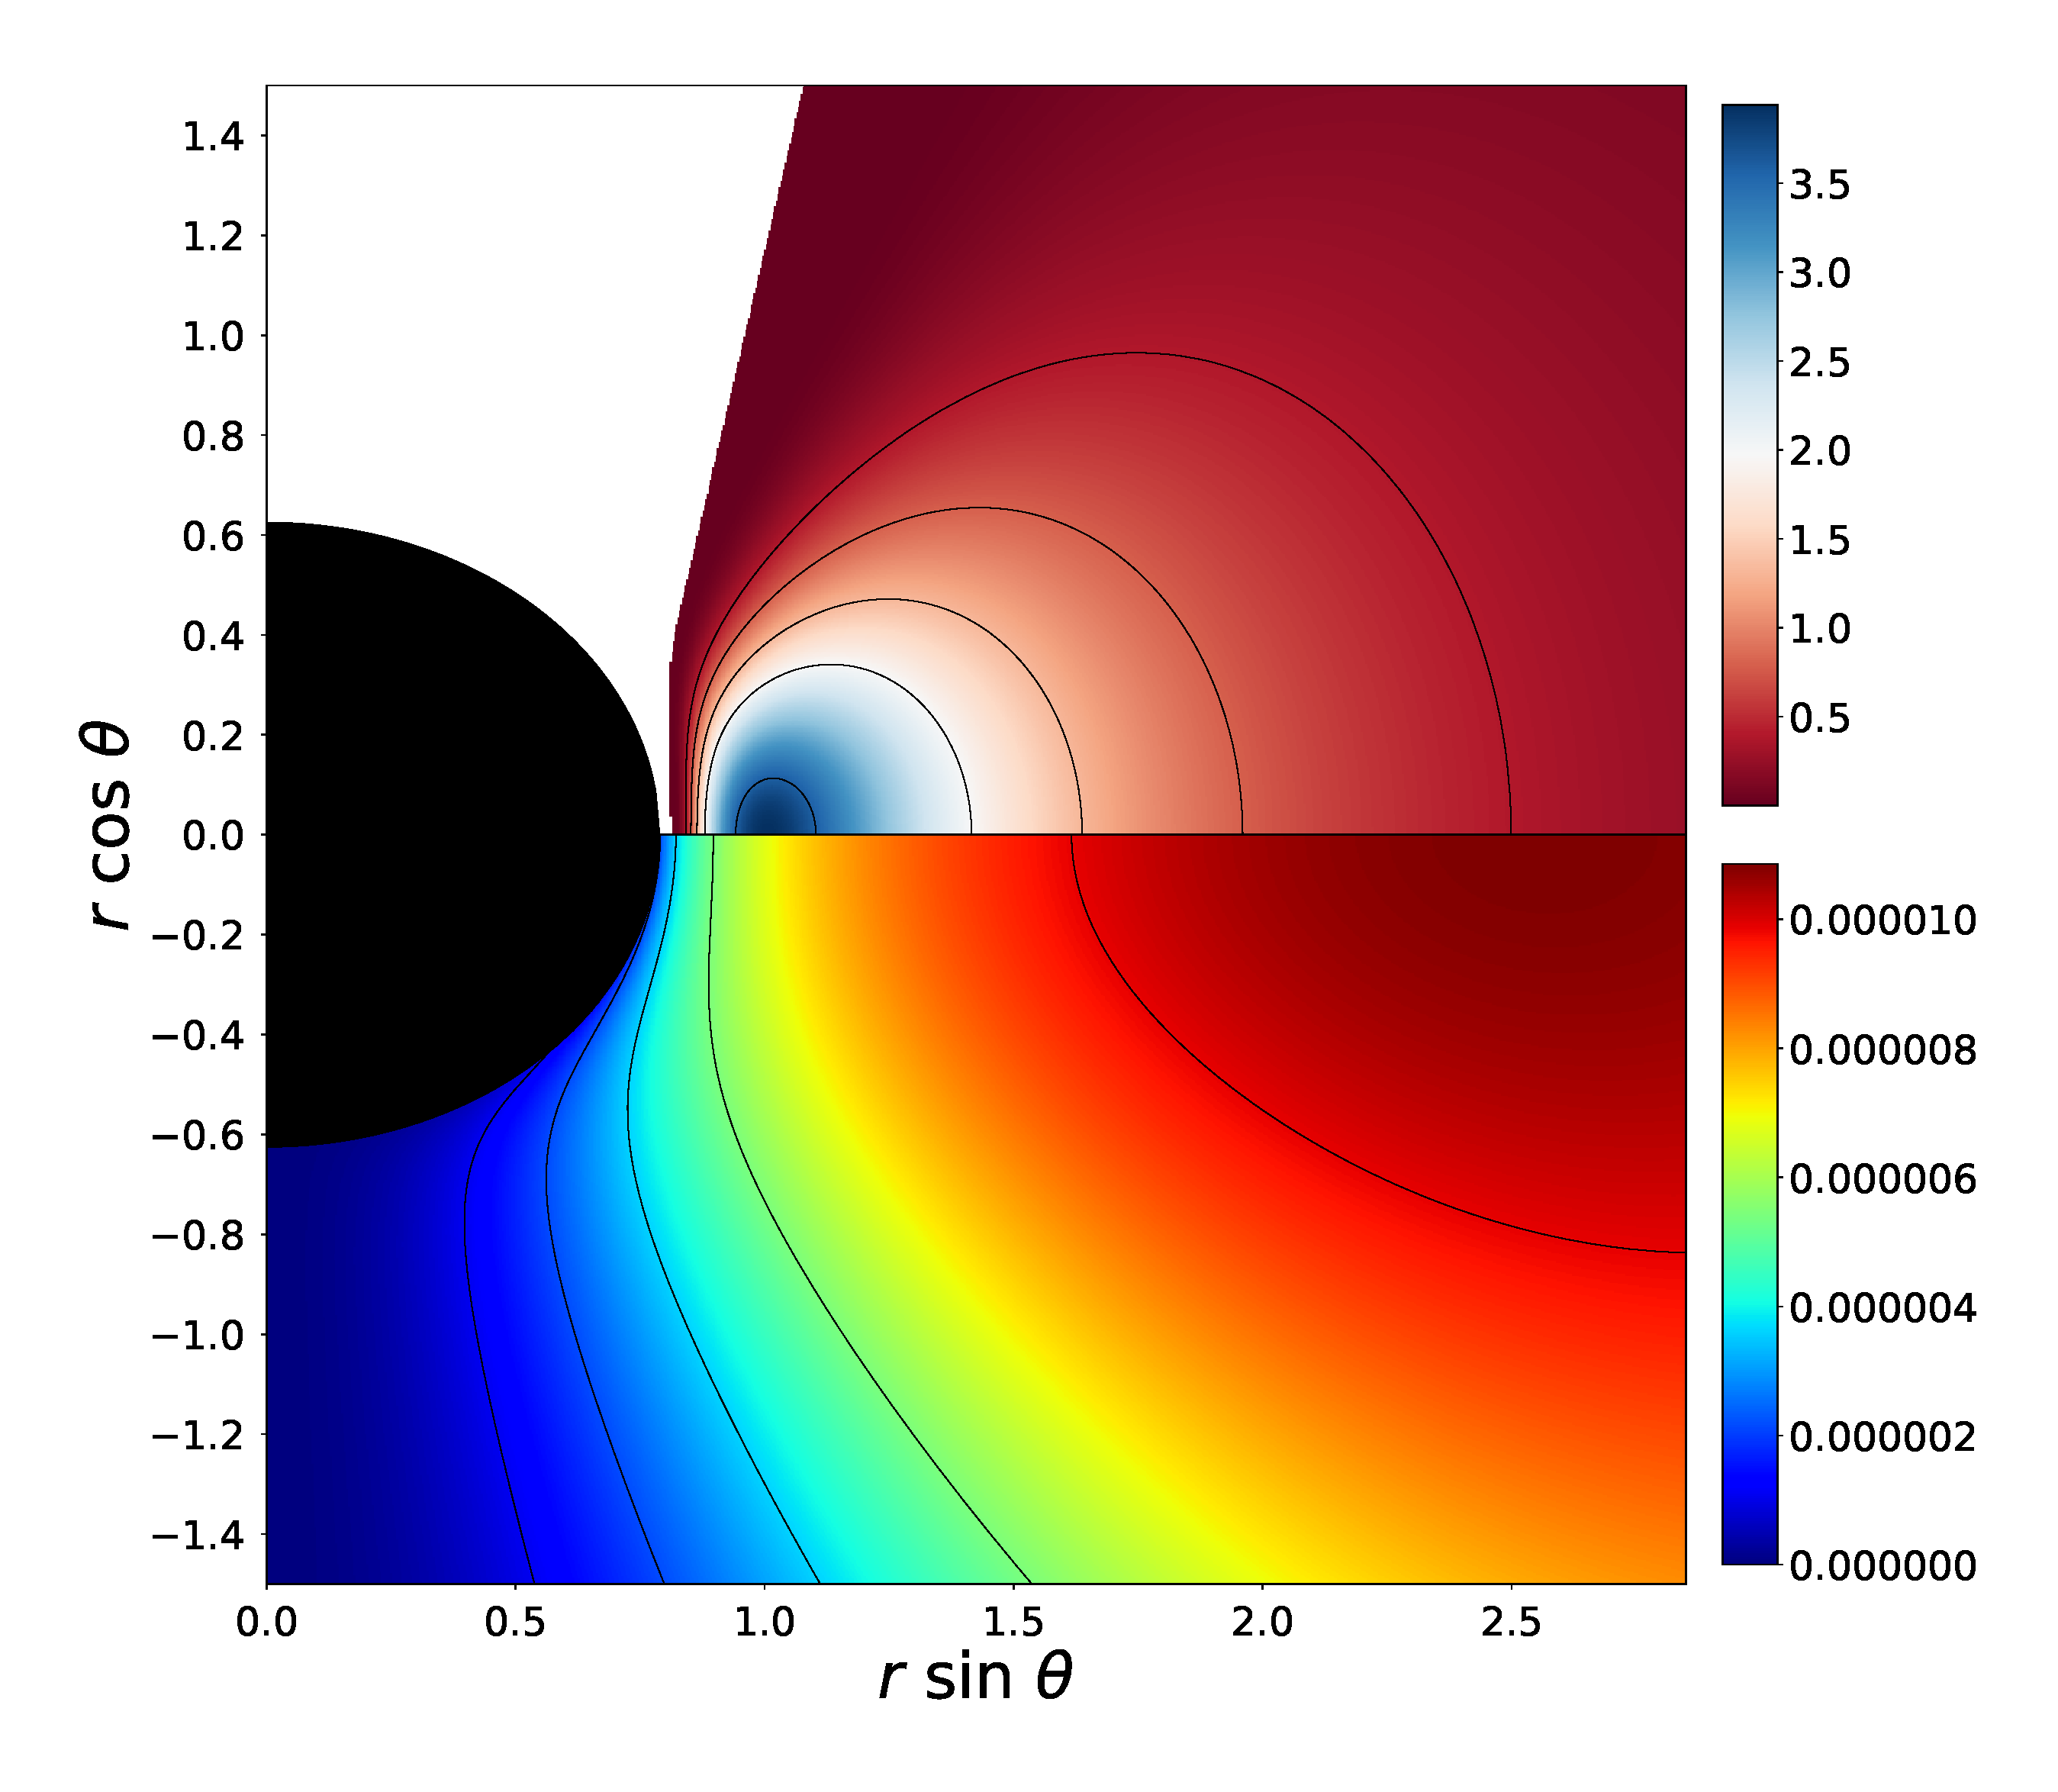
\includegraphics[scale=0.12]{figures/fig6_I_10.pdf}
\hspace{-0.4cm}
\includegraphics[scale=0.12]{figures/fig6_IV_10.pdf}
\hspace{-0.4cm}
\includegraphics[scale=0.12]{figures/fig6_VII_10.pdf}
\hspace{-0.2cm}
\\
\includegraphics[scale=0.12]{figures/fig6_I__10.pdf}
\hspace{-0.4cm}
\includegraphics[scale=0.12]{figures/fig6_IV__10.pdf}
\hspace{-0.4cm}
\includegraphics[scale=0.12]{figures/fig6_VII__10.pdf}
\hspace{-0.2cm}
\caption{Gravitational mass density distribution for the torus $\rho_{\mathrm{T}}$ (up) and the scalar field $\rho_{\mathrm{SF}}$ (down) using perimeteral coordinates. From left to right the columns correspond to different models (I, IV and VII). From top to bottom, the rows correspond to different calues of the magnetization parameter, namely non-magnetized ($\beta_{\mathrm{m}_{\mathrm{c}}} = 10^{10}$) and strongly magnetized ($\beta_{\mathrm{m}_{\mathrm{c}}} = 10^{-10}$)}
\label{comparison_mass_density_peri}
\end{figure*}

\begin{figure*}
\centering
\includegraphics[scale=0.2]{figures/fig7_HBH_dens.eps}
\hspace{-0.cm}
\includegraphics[scale=0.2]{figures/fig7_HBH_enth.eps}
\hspace{-0.cm}
\\
\includegraphics[scale=0.2]{figures/fig7_Kerr_dens.eps}
\hspace{-0.cm}
\includegraphics[scale=0.2]{figures/fig7_Kerr_enth.eps}
\hspace{-0.cm}
\caption{Effects of the magnetization on the values for the maximum density (left) and enthalpy (right) of the disc. In the first row, we show this for all of our KBHsSH models. In the second row, we show this for a sequence of KBHs with increasing spin parameter.}
\label{comparison_HBH_Kerr_dens_enth}
\end{figure*}

\begin{figure*}
\centering
\includegraphics[scale=0.2]{figures/fig8_HBH.eps}
\hspace{0.5cm}
\includegraphics[scale=0.2]{figures/fig8_Kerr.eps}
\hspace{0.5cm}
\caption{Effects of the magnetization on the (perimeteral) location of the magnetic pressure maximum (divided by the the perimeteral radius of the centre)($R_{\mathrm{mag}, \mathrm{max}} / R_{\mathrm{c}}$). Left panel: KBHsSH models. Right panel: A sequence of KBHs with increasing spin parameter.}
\label{comparison_HBH_Kerr_r_m_max}
\end{figure*}

\begin{figure*}
\centering
\includegraphics[scale=0.14]{figures/fig9_0_10.pdf}
\hspace{-0.3cm}
\includegraphics[scale=0.14]{figures/fig9_0_1.pdf}
\hspace{-0.2cm}
\includegraphics[scale=0.14]{figures/fig9_0__10.pdf}
\\
\includegraphics[scale=0.14]{figures/fig9_05_10.pdf}
\hspace{-0.3cm}
\includegraphics[scale=0.14]{figures/fig9_05_1.pdf}
\hspace{-0.2cm}
\includegraphics[scale=0.14]{figures/fig9_05__10.pdf}
\\
\includegraphics[scale=0.14]{figures/fig9_09_10.pdf}
\hspace{-0.3cm}
\includegraphics[scale=0.14]{figures/fig9_09_1.pdf}
\hspace{-0.2cm}
\includegraphics[scale=0.14]{figures/fig9_09__10.pdf}
\\
\includegraphics[scale=0.14]{figures/fig9_09999_10.pdf}
\hspace{-0.3cm}
\includegraphics[scale=0.14]{figures/fig9_09999_1.pdf}
\hspace{-0.2cm}
\includegraphics[scale=0.14]{figures/fig9_09999__10.pdf}
\hspace{-0.2cm}
\caption{Rest-mass density distribution. From top to bottom the rows correspond to a sequence of KBHs with increasing spin parameter $a$ (0, 0.5, 0.9 and 0.9999). From left to right the columns correspond to different values of the magnetization parameter, namely non-magnetized ($\beta_{\mathrm{m}_{\mathrm{c}}} = 10^{10}$), mildly magnetized ($\beta_{\mathrm{m}_{\mathrm{c}}} = 1$) and strongly magnetized ($\beta_{\mathrm{m}_{\mathrm{c}}} = 10^{-10}$)}
\label{models_Kerr}
\end{figure*}

\begin{figure*}
\centering
\includegraphics[scale=0.14]{figures/fig10_0_10.pdf}
\hspace{-0.3cm}
\includegraphics[scale=0.14]{figures/fig10_0_1.pdf}
\hspace{-0.2cm}
\includegraphics[scale=0.14]{figures/fig10_0__10.pdf}
\\
\includegraphics[scale=0.14]{figures/fig10_05_10.pdf}
\hspace{-0.3cm}
\includegraphics[scale=0.14]{figures/fig10_05_1.pdf}
\hspace{-0.2cm}
\includegraphics[scale=0.14]{figures/fig10_05__10.pdf}
\\
\includegraphics[scale=0.14]{figures/fig10_09_10.pdf}
\hspace{-0.3cm}
\includegraphics[scale=0.14]{figures/fig10_09_1.pdf}
\hspace{-0.2cm}
\includegraphics[scale=0.14]{figures/fig10_09__10.pdf}
\\
\includegraphics[scale=0.14]{figures/fig10_09999_10.pdf}
\hspace{-0.3cm}
\includegraphics[scale=0.14]{figures/fig10_09999_1.pdf}
\hspace{-0.2cm}
\includegraphics[scale=0.14]{figures/fig10_09999__10.pdf}
\hspace{-0.2cm}
\caption{Rest-mass density distribution using perimeteral coordinates. From top to bottom the rows correspond to a sequence of KBHs with increasing spin parameter $a$ (0, 0.5, 0.9 and 0.9999). From left to right the columns correspond to different values of the magnetization parameter, namely non-magnetized ($\beta_{\mathrm{m}_{\mathrm{c}}} = 10^{10}$), mildly magnetized ($\beta_{\mathrm{m}_{\mathrm{c}}} = 1$) and strongly magnetized ($\beta_{\mathrm{m}_{\mathrm{c}}} = 10^{-10}$)}
\label{models_Kerr_peri}
\end{figure*}


%%%%%%%%%%%%%%%%%%%%%%%%%%%%%%%%%%%%
\subsection{Distribution of angular momentum in the disk}
%%%%%%%%%%%%%%%%%%%%%%%%%%%%%%%%%%%%

Equilibrium models of disks around Kerr BHs are built assuming that the spacetime metric and the fluid fields are stationary and  axisymmetric.  This was the approach followed in~\cite{Gimeno-Soler:2017}. For KBHsSH we can follow the same approach as the metric ansatz given by Eq.~(\ref{metric}) is stationary and axisymmetric.

%HERE

We start by introducing the specific angular momentum $l$ and the angular velocity $\Omega$ employing the standard definitions,
\begin{equation}
l = - \frac{u_{\phi}}{u_t}, \;\;\; \Omega = \frac{u^{\phi}}{u^t},
\end{equation}
where $u^{\mu}$ is the fluid four-velocity.
The relationship between $l$ and $\Omega$ is given by the equations
\begin{equation}
l = - \frac{\Omega g_{\phi\phi} + g_{t\phi}}{\Omega g_{t\phi} + g_{tt}}, \;\;\; \Omega = - \frac{l g_{tt} + g_{t\phi}}{l g_{t\phi} + g_{\phi\phi}},
\end{equation}
where we are assuming circular motion, i.e.~the four-velocity can be written as
\begin{equation}
u^{\mu} = (u^t, 0, 0, u^{\phi})\,.
\end{equation}

In~\cite{Gimeno-Soler:2017} we followed the approach for the angular momentum distribution given by~\cite{Qian:2009}, which is characterized by the parameters, $\beta$, $\gamma$, and $eta$ (see Eq.~(7) in~\cite{Gimeno-Soler:2017}. In this work, for simplicity and to reduce the space of parameters, we consider a constant angular momentum distribution, $l(r,\theta) = \mathrm{const}$, which corresponds to setting $\beta=\gamma=0$ in ~\cite{Gimeno-Soler:2017}.  \tf{We should explain/motivate why we change our approach in this paper.} The specific value of the angular momentum is computed as the minimum of the following equation
\begin{equation}\label{eq:mb_ang_mom}
l^{\pm}_{\mathrm{b}}(r, \theta) = \frac{g_{t\phi}\pm\left(\sqrt{g_{t\phi}^2-g_{tt}g_{\phi\phi}}\right)\sqrt{1+g_{tt}}}{-g_{tt}}
\end{equation}
where the plus sign is for prograde orbits and the minus is for retrograde orbits.
This expression is given by~\citep{Daigne:2004} for Kerr BHs, but it is valid for any stationary, axisymmetric spacetimes. For prograde motion, the function has a minimum outside the event horizon. The location of said minimum corresponds with the marginally bound orbit $r_{\mathrm{mb}}$, and the angular momentum corresponds to the keplerian angular momentum $l_{\mathrm{mb}}$ at that point. We show the proof of this statement at appendix~\ref{ang_mom_appendix}. This choice of angular momentum distribution is motivated by its simplicity (for a first study of thick tori around KBHsSH) and for allowing the presence of a cusp (to allow matter accretion onto the black hole) and a centre.

%%%%%%%%%%%%%%%%
\subsection{Magnetized disks}
%%%%%%%%%%%%%%%%

We use the procedure described by~\cite{Montero:2007}, where we write the equations of ideal general relativistic MHD as the following conservation laws, $\nabla_{\mu} T^{\mu\nu} = 0$, $\nabla_{\mu} \,^\ast F^{\mu\nu} = 0$, and 
$\nabla_{\mu} (\rho u^{\mu}) = 0$, 
where $\nabla_{\mu}$ is the covariant derivative and
\begin{equation}\label{eq:e-m_tensor}
T^{\mu\nu} = (\rho h + b^2)u^{\mu}u^{\nu} + \left(p + \frac{1}{2}b^2\right)g^{\mu\nu} - b^{\mu}b^{\nu},
\end{equation}
is the energy-momentum tensor of a magnetised perfect fluid, $h$, $\rho$ $p$ being the fluid specific enthalpy, density and fluid pressure, respectively. 
Moreover, $^\ast F^{\mu\nu} = b^{\mu}u^{\nu} - b^{\nu}u^{\mu}$ is the (dual of the) Faraday tensor relative to an observer with 
four-velocity $u^{\mu}$, and $b^{\mu}$ is the magnetic field in that frame, with
$b^2=b^{\mu}b_{\mu}$. Assuming the magnetic field is purely azimuthal, i.e.~$b^r = b^{\theta} = 0$,
and taking into account that the flow is stationary and axisymmetric, the conservation of the current density and of the Faraday tensor follow. Contracting the divergence of Eq.~\eqref{eq:e-m_tensor} with the projection tensor $h^{\alpha}_{\,\,\beta} = \delta^{\alpha}_{\,\,\beta} + u^{\alpha}u_{\beta}$, we arrive at
\begin{equation}
(\rho h + b^2)u_{\nu}\partial_i u^{\nu} + \partial_i\left(p + \frac{b^2}{2}\right) - b_{\nu}\partial_i b^{\nu}=0\,,
\end{equation}
where $i = r, \theta$. Then, we rewrite this equation in terms of the specific angular momentum $l$ and of the angular velocity $\Omega$, to obtain
\begin{equation}\label{eq:diff_ver}
\partial_i(\ln u_t|) - \frac{\Omega \partial_i l}{1-l\Omega} + \frac{\partial_i p}{w} + \frac{\partial_i(\mathcal{L}b^2)}{2\mathcal{L}w} = 0\,,
\end{equation}
where $\mathcal{L} = g_{t\phi}^2 - g_{tt}g_{\phi\phi}$.

To integrate Eq.~\eqref{eq:diff_ver} we first assume a polytropic equation of state of the form
\begin{equation}\label{eq:eos_fluid}
p = K \rho^{\Gamma},
\end{equation}
with $K$ and $\Gamma$ constants.
Then, we define the magnetic pressure as $p_{\mathrm{m}} = b^2/2$, the magnetization parameter $\beta_{\mathrm{m}} = p/p_{\mathrm{m}}$, and introduce the definitions $\tilde{p}_{\mathrm{m}} = \mathcal{L} p_{\mathrm{m}}$ and $\tilde{w} = \mathcal{L} w$, in order to write an analogous equation to Eq.~\eqref{eq:eos_fluid} for $\tilde{p}_{\mathrm{m}}$
\begin{equation}\label{eq:eos_mag_tilde}
\tilde{p}_{\mathrm{m}} = M \tilde{w}^q,
\end{equation}
or, in terms of the magnetic pressure $p_{\mathrm{m}}$
\begin{equation}\label{eq:eos_mag}
p_{\mathrm{m}} = M \mathcal{L}^{q-1} w^q,
\end{equation}
where $w = \rho h$ is the fluid enthaply density, and $M$ and $q$ are constants.
If we define the potential as $W \equiv \ln |u_t|$, then we can integrate the equation~\eqref{eq:diff_ver} as
\begin{equation}\label{eq:final}
W - W_{\mathrm{in}} + \ln \left(1 + \frac{\Gamma K}{\Gamma +1}\rho^{\Gamma -1}\right) + \frac{q}{q-1}M(\mathcal{L}w)^{q-1}=0,
\end{equation}
where $W_{\mathrm{in}}$ is the potential at the inner edge of the disk.

We also write the expressions of the total energy density for the torus $\rho_{\mathrm{T}}$:
\begin{equation}\label{eq:torus_energy_density}
\rho_{\mathrm{T}} = -T^t_t + T^i_i = \frac{\rho h (g_{\phi\phi} - g_{tt} l^2)}{g_{\phi\phi} + 2 g_{t\phi} l + g_{tt} l^2} + 2 (p + p_{\mathrm{m}}),
\end{equation}
and the total energy density for the scalar field $\rho_{\mathrm{SF}}$:
\begin{equation}\label{eq:SF_energy_density}
\rho_{\mathrm{SF}} = -(T_{\mathrm{SF}})^t_t + (T_{\mathrm{SF}})^i_i = 2 \left(\frac{2 e^{2 F_0} w (w-m W)}{N} - \mu^2\right) \phi^2.
\end{equation}

In this work, we set the mass of the scalar field $\mu = 1$, the angular momentum to $l = l_{\mathrm{mb}}$, the inner radius of the disk to $r_{\mathrm{in}} = r_{\mathrm{mb}}$, the exponents of the polytropic EoS to $q = \Gamma = 4/3$, and the density at the disk centre $\rho_{\mathrm{c}} = 1$. Then, we leave the magnetization at the center $\beta_{\mathrm{m_c}}$ as a parameter (for each model of KBHSH). With this information we can compute all the relevant physical quantities.

%%%%%%%%%%%%
\section{Methodology}
\label{procedure}
%%%%%%%%%%%%

%%%%%%%%%%%%%%%%
\subsection{Building the disk}
%%%%%%%%%%%%%%%%

To construct our models we take the following steps:
First, we find the angular momentum $l$ and the radius of the cusp $r_{\mathrm{cusp}}$ as the value at the minimum and the location of said minimum outside the event horizon of equation~\eqref{eq:mb_ang_mom}. This choice of angular momentum implies $r_{\mathrm{cusp}} = r_{\mathrm{mb}}$, $l = l_{\mathrm{K}}(r_{\mathrm{mb}})$ and $W_{\mathrm{in}} = 0$ and then, we can compute the potential distribution as $W(r, \theta) \equiv \ln |u_t|$. Considering this, and that we can write the magnetic pressure at the center as
\begin{equation}
p_{\mathrm{m_c}} = M \mathcal{L}^{q-1} \left(1 + \frac{\Gamma K}{\Gamma +1}\right)^q = K/\beta_{\mathrm{m_c}},
\end{equation}
where we have taken into account that $\rho_{\mathrm{c}} = 1$, that the pressure at the center is $p_{\mathrm{c}} = K$ and the specific enthalpy can be written as $h = 1 + \frac{\Gamma K}{\Gamma +1}\rho^{\Gamma -1}$. Replacing this into the equation~\eqref{eq:final} we arrive at an equation for the polytropic constant $K$
\begin{equation}\label{eq:K_eq}
W_{\mathrm{c}} + \ln \left(1 + \frac{\Gamma K}{\Gamma +1}\right) + \frac{q}{q-1}\frac{K/\beta_{\mathrm{m_c}}}{1 + \frac{\Gamma K}{\Gamma +1}} = 0.
\end{equation}
Once we have $K$, it is easy to find $p_{\mathrm{m}}$, $M$ and $h_{\mathrm{c}}$ with the definition of the magnetization parameter at the center $\beta_{\mathrm{m_c}}$, the equation~\eqref{eq:eos_mag} and $h = 1 + \frac{\Gamma K}{\Gamma +1}\rho^{\Gamma -1}$. With this, we already have all we need in order to compute all the relevant physical quantities inside the disk.

%%%%%%%%%%%%%%%%%
\subsection{Numerical method}
%%%%%%%%%%%%%%%%%

We start from a uniform numerical grid $(X, \theta)$ (with $x$ being a compactified radial coordinate such as $X = x/(1+x)$ and $x = \sqrt{r^2 - r_{\mathrm{H}}^2}$) with a domain $[0, 1] \times [0, \pi/2]$ and a number of points of $N_X \times N_\theta = 251 \times 30$. Then, we transform and interpolate the grid to end with a non-uniform grid $(r, \theta)$ with a domain $[r_{\mathrm{H}}, 199.2] \times [0, pi/2]$ and a number of points $N_r \times N_\theta = 2500 \times 300$, this is the grid we use for our computations.

%%%%%%%%%%
\section{Results}
\label{results}
%%%%%%%%%%

%In table~\ref{models_list} we show the different KBHsSH models we will use. As it can be seen, the models go from a Kerr-like model (almost all the mass and angular momentum are stored in BH) to a KBHSH with almost all the mass and angular momentum stored in the scalar field. It is also worth mentioning that, as shown in table~\ref{models_spin_vel} some of the models violate the Kerr bound (in terms of ADM or horizon quantities). This is not worrying because, as shown in~\cite{Herdeiro:2015c} the horizon linear velocity $v_{\mathrm{H}}$ never exceed $1$. For comparison, we also show the spin parameter $a_{\mathrm{H_{eq}}}$ corresponding to a Kerr BH with horizon linear velocity $v_{\mathrm{H}}$.

In figures~\ref{models_I} and~\ref{models_II} we show the rest-mass density distribution for all our KBHsSH models with 3 different values of the magnetization parameter at the center $\beta_{\mathrm{m_c}}$, namely $10^{10}$, $1$ and $10^{-10}$. In figures~\ref{models_peri_I} and~\ref{models_peri_II} we show the same models, but using a perimeteral radial coordinate such as $R = e^{F_2} r$. Also, in figures~\ref{models_Kerr} and~\ref{models_Kerr_peri} we show different KBH models with the same mass $M_{\mathrm{BH}} = 1$ and different values for the spin parameter($0$, $0.5$, $0.9$, $0.9999$). Tables~\ref{HBH_disk_parameters} and~\ref{KBH_disk_parameters} show the relevant physical quantities for both KBHSH and the same KBH cases we presented in the figures. First of all, it is worth to mention that KBHsSH can violate the Kerr bound for the potential $\Delta W \equiv W_{\mathrm{in}} - W_{\mathrm{c}}$. As shown in~\cite{Abramowicz:1978}, constant angular momentum disks exhibit a maximum for $|\Delta W|$ when the spin parameter $a$ approaches 1. This value is $\Delta W_{\mathrm{max}} = -\frac{1}{2} \ln 3 \simeq -0.549$. The models V, VI and VII violate that bound. This is related, as we will see, with the maximum value of the specific enthalpy, pressure and magnetic pressure.

In figure~\ref{comparison_mass_density} we show the total energy density of the torus $\rho_{\mathrm{T}}$ (superior half) and the total energy density of the scalar field $\rho_{\mathrm{SF}}$ for 3 of the models (I, IV and VII) and 2 values of the magnetization parameter at the center ($10^{10}$ and $10^{-10}$). In figure~\ref{comparison_mass_density_peri}, we show the same, but using the perimeteral coordinate we defined earlier. The plots show that the maximum of the total energy density of the disk $\rho_{\mathrm{t}}$ is closer to the maximum of the total energy density of the scalar field $\rho_{\mathrm{SF}}$ for increasing hair.

The behaviour of the maximum specific enthalpy $h_{\mathrm{max}}$ and the maximum rest-mass density $\rho_{\mathrm{max}}$ is shown in figures~\ref{comparison_HBH_Kerr_dens_enth} for the models (I-VII) and for a sequence of increasing spin parameter KBHs, here we can see that, for both cases, an increase in $|\Delta W|$ implies higher values for $h_{\mathrm{max}}$ (low magnetization) and also higher values for $\rho_{\mathrm{max}}$ (high magnetization). However, there are differences between the two cases. For the enthalpy, the values of $h_{\mathrm{max}}$ reached for the KBHsSH are much higher than those of the KBH case. This fact tells us that, while the $w = \rho h \simeq \rho$ approximation (see \cite{Komissarov:2006} and \cite{Gimeno-Soler:2017}) is valid for magnetized flows ($\beta_{\mathrm{m_c}} \sim 1$) for reasonable values of the spin parameter ($a \sim 0.99$ or lower), that is not the case for KBHsSH. Also, for the rest-mass density we have a different behaviour: $\rho_{\mathrm{max}}$ for KBHsSH reach values only attainable by high spin parameter KBHs (between $a = 0.9$ and $a = 0.99999$ for the seven models we present here).

Figure~\ref{comparison_HBH_Kerr_r_m_max} shows the variation of the quotient of the perimeteral radius of the magnetic pressure maximum by the perimeteral radius of the disk center $R_{\mathrm{m, max}}/R_{\mathrm{c}}$ with the decimal logarithm of the magnetization parameter at the disk center $\log_{10} \beta_{\mathrm{m_c}}$ for the same KBHsSH and KBH cases as in figure~\ref{comparison_HBH_Kerr_dens_enth}. The inset shows a region around $\beta_{\mathrm{m_c}} = 3$ and $R_{\mathrm{m, max}}/R_{\mathrm{c}} = 1$, this is because for disks with $h = 1$, $R_{\mathrm{m, max}} = R_{\mathrm{c}}$ if $\beta_{\mathrm{m_c}} = 1 / \Gamma - 1$. As we can easily see, this condition is also fulfilled for the Kerr case, even $h \neq 1$ (with a slight deviation for very high spin parameter cases), but not quite for the KBHsSH cases.

\sg{Include discussion about radial profiles.}

As shown in~\cite{Delgado:2018} some \sg{(compute which ones are embeddable and which are not)} of our models are in the region of the domain of existence where the event horizon is not embeddable in $\mathbb{E}^3$ then, the shaded regions depicting the horizon that we show at several of the figures are not faithful representations of the horizon geometry. Nevertheless, we show them for the sake of clarity. Also, this led us to asking ourselves if this could also happen for the shape of the accretion tori and therefore, we should be conservative when extracting information about the morphology of the disks from 2-dimensional plots. This idea is discussed in appendix~\ref{torus_embedding}.

%\begin{table}
%\caption{List of models of KBHsSH.}        
%\label{models_list}      
%\centering          
%\begin{tabular}{c c c c  c c c c}
%\hline\hline       
% Model & $M_{\mathrm{ADM}}$ & $J_{\mathrm{ADM}}$ & $M_{\mathrm{H}}$ &  $J_{\mathrm{H}}$ & $M_{\mathrm{SF}}$ & $J_{\mathrm{SF}}$ & $r_{\mathrm{H}}$ \\ 
%\hline           
%I & $0.415$ & $0.172$ & $0.393$ &  $0.15$  & $0.022$ & $0.022$ & $0.2$\\ 
% \hline 
%II & $0.630$ & $0.403$ & $0.340$ &  $0.121$  & $0.063$ & $0.282$ & $0.221$ \\
% \hline 
%III & $0.797$ & $0.573$ & $0.365$ &  $0.172$  & $0.573$ & $0.432$ & $0.111$ \\ 
% \hline 
%IV & $0.933$ & $0.739$ & $0.234$ &  $0.114$  & $0.699$ & $0.625$ & $0.1$ \\ 
% \hline 
%V & $0.940$ & $0.757$ & $0.159$ &  $0.076$  & $0.757$ & $0.781$ & $0.091$ \\ 
% \hline 
%VI & $0.959$ & $0.795$ & $0.087$ &  $0.034$  & $0.872$ & $0.781$ & $0.088$ \\ 
% \hline 
%VII & $0.975$ & $0.85$ & $0.018$ &  $0.002$  & $0.957$ & $0.848$ & $0.04$ \\ 
%\hline      
%\end{tabular}
%\end{table}
%
%\begin{table}
%\caption{Values of the normalized spin parameter for the ADM quantities ($a_{\mathrm{ADM}}$), for the BH horizon quantities ($a_{\mathrm{H}}$), the horizon linear velocity ($v_{\mathrm{H}}$) and the spin parameter corresponding to a KBH with a linear velocity equal to $v_{\mathrm{H}}$, ($a_{\mathrm{H_{eq}}}$).}        
%\label{models_spin_vel}      
%\centering          
%\begin{tabular}{c c c c c}
%\hline\hline       
% Model & $a_{\mathrm{ADM}}$ & $a_{\mathrm{H}}$ & $v_{\mathrm{H}}$ & $a_{\mathrm{H_{eq}}}$ \\ 
%\hline           
%I & $0.9987$ & $0.9712$ & $0.7685$ & $0.9663$ \\ 
% \hline 
%II & $1.014$ & $0.3760$ & $0.6802$ & $0.9301$ \\
% \hline 
%III & $0.9032$ & $1.295$ & $0.7524$ & $0.9608$ \\ 
% \hline 
%IV & $0.8489$ & $2.082$ & $0.5635$ & $0.8554$ \\ 
% \hline 
%V & $0.8560$ & $3.017$ & $0.4438$ & $0.7415$ \\ 
% \hline 
%VI & $0.9477$ & $3.947$ & $0.2988$ & $0.5487$ \\ 
% \hline 
%VII & $0.8941$ & $6.173$ & $0.09732$ & $0.1928$ \\ 
%\hline      
%\end{tabular}
%\end{table}

\begin{table*}[t]
\caption{Disk parameters and values of their relevant physical magnitudes. For all the cases, we have $R_{\mathrm{in}} = R_{\mathrm{mb}}$ and $l = l_{\mathrm{mb}}$}        
\label{HBH_disk_parameters}      
\centering          
\begin{tabular}{c c c c c  c c c c c c c}
\hline\hline       
 Model & $l$ & $W_{\mathrm{c}}$ & $R_{\mathrm{in}}$ & $R_{\mathrm{c}}$ &  $\beta_{\mathrm{m_{\mathrm{c}}}}$ & $h_{\mathrm{max}}$ & $\rho_{\mathrm{max}}$ & $p_{\mathrm{max}}$ & $p_{\mathrm{m, max}}$ & $R_{\mathrm{max}}$ & $R_{\mathrm{m, max}}$\\ 
\hline           
I & $0.934$ & $-0.188$ & $0.81$ & $1.14$ & $10^{10}$ & $1.21$ & $1.0$ & $5.16 \times 10^{-2}$ & $5.50 \times 10^{-12}$ & $1.14$ & $1.26$\\ 
 \hline 
 &  &  &  &  & $1$ & $1.10$ & $1.17$ & $3.11 \times 10^{-2}$ & $2.68 \times 10^{-2}$ & $1.01$ & $1.06$\\ 
 \hline 
 &  &  &  &  & $10^{-10}$ & $1.0$ & $1.90$ & $1.10 \times 10^{-11}$ & $7.80 \times 10^{-2}$ & $0.93$ & $0.96$\\ 
 \hline 
II & $0.933$ & $-0.205$ & $0.75$ & $1.18$ & $10^{10}$ & $1.23$ & $1.0$ & $5.69 \times 10^{-2}$ & $6.14 \times 10^{-12}$ & $1.18$ & $1.36$\\ 
 \hline 
 &  &  &  &  & $1$ & $1.12$ & $1.19$ & $3.50 \times 10^{-2}$ & $2.97 \times 10^{-2}$ & $1.00$ & $1.07$\\ 
 \hline 
 &  &  &  &  & $10^{-10}$ & $1.0$ & $2.01$ & $1.30 \times 10^{-11}$ & $8.99 \times 10^{-2}$ & $0.91$ & $0.94$ \\ 
 \hline 
III & $1.06$ & $-0.362$ & $0.84$ & $1.07$ & $10^{10}$ & $1.44$ & $1.0$ & $0.109$ & $1.21 \times 10^{-11}$ & $1.07$ & $1.22$\\ 
 \hline 
 &  &  &  &  & $1$ & $1.23$ & $1.28$ & $7.22 \times 10^{-2}$ & $5.76 \times 10^{-2}$ & $0.95$ & $0.99$ \\ 
 \hline 
 &  &  &  &  & $10^{-10}$ & $1.0$ & $2.74$ & $3.48 \times 10^{-11}$ & $0.206$ & $0.89$ & $0.91$\\ 
\hline  
IV & $1.16$ & $-0.547$ & $0.67$ & $1.06$ & $10^{10}$ & $1.723$ & $1.0$ & $0.182$ & $2.09 \times 10^{-11}$ & $1.06$ & $1.34$ \\ 
\hline 
 &  &  &  &  & $1$ & $1.38$ & $1.37$ & $0.129$ & $9.76 \times 10^{-2}$ & $0.85$ & $0.91$\\ 
\hline 
 &  &  &  &  & $10^{-10}$ & $1.0$ & $3.70$ & $7.83 \times 10^{-11}$ & $0.408$ & $0.76$ & $0.78$ \\ 
\hline   
V & $1.20$ & $-0.685$ & $0.58$ & $1.07$ & $10^{10}$ & $1.98$ & $1.0$ & $0.246$ & $2.76 \times 10^{-11}$ & $1.07$ & $1.31$\\ 
\hline 
 &  &  &  &  & $1$ & $1.51$ & $1.40$ & $0.178$ & $0.132$ & $0.78$ & $0.87$ \\ 
\hline 
 &  &  &  &  & $10^{-10}$ & $1.0$ & $4.26$ & $1.18 \times 10{-10}$ & $0.579$ & $0.67$ & $0.69$ \\ 
\hline   
VI & $1.20$ & $-0.832$ & $0.43$ & $1.12$ & $10^{10}$ & $2.30$ & $1.0$ & $0.324$ & $3.52 \times 10^{-11}$ & $1.12$ & $1.32$ \\ 
\hline 
 &  &  &  &  & $1$ & $1.66$ & $1.39$ & $0.228$ & $0.169$ & $0.72$ & $0.86$ \\ 
\hline 
 &  &  &  &  & $10^{-10}$ & $1.0$ & $4.54$ & $1.57 \times 10^{-10}$ & $0.740$ & $0.55$ & $0.59$ \\ 
\hline 
VII & $0.920$ & $-1.236$ & $0.18$ & $1.10$ & $10^{-10}$ & $3.44$ & $1.0$ & $0.610$ & $6.459 \times 10^{-11}$ & $1.10$ & $1.25$ \\ 
\hline 
 &  &  &  &  & $1$ & $2.25$ & $1.64$ & $0.510$ & $0.322$ & $0.43$ & $0.62$\\ 
\hline 
 &  &  &  &  & $10^{-10}$ & $1.0$ & $10.42$ & $7.03 \times 10^{-10}$ & $2.44$ & $0.28$ & $0.30$\\ 
\hline 
\end{tabular}
\end{table*}

\begin{table*}[t]
\caption{Disc parameters and values of their relevant physical magnitudes for the KBH case. For all the cases, we have $R_{\mathrm{in}} = R_{\mathrm{mb}}$ , $l = l_{\mathrm{mb}}$ and $M_{\mathrm{BH}} = 1$.}        
\label{KBH_disk_parameters}      
\centering          
\begin{tabular}{c c c c c  c c c c c c c}
\hline\hline       
 $a$ & $l$ & $W_{\mathrm{c}}$ & $R_{\mathrm{in}}$ & $R_{\mathrm{c}}$ &  $\beta_{\mathrm{m_{\mathrm{c}}}}$ & $h_{\mathrm{max}}$ & $\rho_{\mathrm{max}}$ & $p_{\mathrm{max}}$ & $p_{\mathrm{m, max}}$ & $R_{\mathrm{max}}$ & $R_{\mathrm{m, max}}$\\ 
\hline           
$0$ & $4.00$ & $-4.32 \times 10^{-2}$ & $4.00$ & $10.47$ & $10^{10}$ & $1.04$ & $1.0$ & $1.10 \times 10^{-2}$ & $1.15 \times 10^{-12}$ & $10.47$ & $11.86$\\ 
 \hline 
 &  &  &  &  & $1$ & $1.02$ & $1.11$ & $6.29 \times 10^{-3}$ & $5.69 \times 10^{-3}$ & $8.81$ & $9.52$\\ 
 \hline 
 &  &  &  &  & $10^{-10}$ & $1.0$ & $1.48$ & $1.83 \times 10^{-12}$ & $1.48 \times 10^{-2}$ & $7.70$ & $8.14$\\ 
 \hline 
 $0.5$ & $3.41$ & $-6.35 \times 10^{-2}$ & $2.99$ & $7.12$ & $10^{10}$ & $1.07$ & $1.0$ & $1.64 \times 10^{-2}$ & $1.72 \times 10^{-12}$ & $7.19$ & $8.14$\\ 
 \hline 
 &  &  &  &  & $1$ & $1.03$ & $1.12$ & $9.43 \times 10^{-3}$ & $8.47 \times 10^{-3}$ & $6.05$ & $6.53$ \\ 
 \hline 
 &  &  &  &  & $10^{-10}$ & $1.0$ & $1.53$ & $2.81 \times 10^{-12}$ & $2.23 \times 10^{-2}$ & $5.29$ & $5.59$\\ 
\hline  
$0.9$ & $2.63$ & $-0.129$ & $2.18$ & $3.78$ & $10^{10}$ & $1.14$ & $1.0$ & $1.64 \times 10^{-2}$ & $3.65 \times 10^{-12}$ & $3.78$ & $4.23$\\ 
 \hline 
 &  &  &  &  & $1$ & $1.07$ & $1.14$ & $2.03 \times 10^{-2}$ & $1.78 \times 10^{-2}$ & $3.25$ & $3.47$\\ 
 \hline 
 &  &  &  &  & $10^{-10}$ & $1.0$ & $1.70$ & $6.54 \times 10^{-12}$ & $4.92 \times 10^{-2}$ & $2.92$ & $3.04$ \\ 
 \hline 
$0.9999$ & $2.02$ & $-0.429$ & $2.00015$ & $2.034$ & $10^{10}$ & $1.54$ & $1.0$ & $0.134$ & $1.61 \times 10^{-11}$ & $2.034$ & $2.094$ \\ 
\hline 
 &  &  &  &  & $1$ & $1.29$ & $1.51$ & $0.110$ & $7.52 \times 10^{-2}$ & $2.0075$ & $2.014$\\ 
\hline 
 &  &  &  &  & $10^{-10}$ & $1.0$ & $6.17$ & $1.22 \times 10^{-10}$ & $0.491$ & $2.0021$ & $2.0030$ \\ 
\hline   
\end{tabular}
\end{table*}

%%%%%%%%%%%%
\section{Conclusions}
\label{conclusions}
%%%%%%%%%%%%

Future work: Non-constant angular momentum case, Proca hair, shadows of the system HBH+disk.

\begin{acknowledgements}

\end{acknowledgements}

\bibliographystyle{apsrev4-1}
\bibliography{references.bib}

\begin{appendix}
\section{Embedding of the accretion torus in $\mathbb{E}^3$}\label{torus_embedding}
Following the same reasoning as in~\cite{Delgado:2018}, we write the 2-metric for the surface of a torus as 
\begin{equation}\label{eq:torus_prev_metric}
\mathrm{d}\sigma^2 = \frac{e^{2 F_1}}{N}\mathrm{d}r^2+ e^{2 F_1}r^2\mathrm{d}\theta^2+e^{2 F_2} r^2 \sin^2\theta \mathrm{d}\phi^2,
\end{equation}
and the condition $r = r(\theta)$ for the surface of the torus. The location of the surface of the torus $r(\theta)$ can be obtained integrating $r' = \frac{\mathrm{d}r}{\mathrm{d}\theta} = -\frac{\partial_{\theta}W}{\partial_{r}W}$ (equation (24) of~\citep{Gimeno-Soler:2017}). Using this, we can write equation~\eqref{eq:torus_prev_metric} as
\begin{equation}\label{eq:torus_metric}
\mathrm{d}\sigma^2 = e^{2 F_1} \mathrm{d}\theta^2\left(\frac{r'^2}{N} +r^2\right)+e^{2 F_2} r^2 \sin^2\theta \mathrm{d}\phi^2,
\end{equation}
with the prime $'$ denoting partial differentiation with respect to $\theta$. Then, we try the embedding in $\mathbb{E}^3$ with the Cartesian metric $\mathrm{d}\sigma^2 = \mathrm{d}X^2 + \mathrm{d}Y^2 + \mathrm{d}Z^2$ and the embedding functions:
\begin{equation}
X + \mathrm{i}Y = f(\theta)e^{\mathrm{i}\phi},  \;\;\; Z = g(\theta),
\end{equation}
then
\begin{equation}
f = e^{2 F_2} r^2 \sin^2\theta, \;\;\; f'^2 + g'^2 = e^{2 F_1}\left(\frac{r'^2}{N} +r^2\right),
\end{equation}
so we can write $g'^2$ as
\begin{equation}\label{eq:embedding_existance}
g'^2 = e^{2 F_1}\left(\frac{r'^2}{N} +r^2\right) - e^{2 F_2} (F_2'r \sin \theta + r' \sin \theta + r \cos \theta)^2.
\end{equation}
This result tells us that the r.h.s. of~\eqref{eq:embedding_existance} must be $\geq 0$ in order to the embedding function to exist.

\begin{figure*}
\centering
\includegraphics[scale=0.2]{figures/embedding.pdf}
\hspace{0.5cm}
\caption{Rest-mass density distribution for model VII with $r_{\mathrm{in}} = 0.08$ and $\beta_{\mathrm{m_c}} = 10^{10}$ (up) and the scalar field amplitude distribution $\phi$ (down). The isocontours are blue when the r.h.s. of equation~\eqref{eq:embedding_existance} is $> 0$ and red when is $\leq 0$.}
\label{embedding_VII}
\end{figure*}

\section{Finding $l_{\mathrm{mb}}$ and $r_{\mathrm{mb}}$}\label{ang_mom_appendix}
\sg{To do.}
\end{appendix}     

\end{document}


